\chapter{有序集，基数，整数}

\section{序关系。有序集}

\subsection{序关系的定义}

设 \(\mathbb{R}\{x, y\}\) 为一个关系，其中 \(x\) 与 \(y\) 是不同的字母。 \(\mathbb{R}\) 被称为关于字母 \(x\) 与 \(y\) （或介于 \(x\) 与 \(y\) 之间）的一个序关系，如果

\[
(R \{x, y \} \text {   且   } R \{y, z \}) \Longrightarrow R \{x, z \},
\]

\[
(\mathrm{R} \{x, y \} \text {   且   } \mathrm{R} \{y, x \}) \Longrightarrow (x = y),
\]

\[
\mathrm{R} \left\{x, y \right\} \Longrightarrow (\mathrm{R} \left\{x, x \right\} \text { 且 } \mathrm{R} \left\{y, y \right\}).
\]

上述关系中的第一个表明，R关于字母x和y是传递的（第二章，§6，第1节）。

示例

\begin{enumerate}
\def\labelenumi{(\arabic{enumi})}
\item
  相等关系， \(x = y\) 是一个序关系。
\item
  关系 \(X \subset Y\) 是X与Y之间的一个序关系（第二章，§1，第2号，命题1和2以及公理A1），通常称为包含关系。
\item
  设 \(\mathbf{R}\{x, y\}\) 为 \(x\) 与 \(y\) 之间的一个序关系。关系 \(\mathbf{R}\{y, x\}\) 则是 \(x\) 与 \(y\) 之间的一个序关系，称为序关系 \(\mathbf{R}\{x, y\}\) 的相反关系。
\end{enumerate}

集合 E 上的一个序关系就是序关系 \(R\{x, y\}\) 关于两个不同的字母 x, y，使得关系 \(R\{x, x\}\) 等价于 \(x \in E\) （换言之，即满足 \(R\{x, y\}\) 在 E 上是自反的（第二章，§6，第 1 号））。则关系 \(R\{x, y\}\) 蕴含“ \(x \in E\) 并且 \(y \in E\) '' 以及关系 \((R\{x, y\}\) 并且 \(R\{y, x\})\) 等价于“ \(x \in E\) 并且 \(y \in E\) 并且 \(x = y\) ''.

示例

\begin{enumerate}
\def\labelenumi{(\arabic{enumi})}
\item
  相等关系和包含关系并不是集合上的序关系，因为这些关系 \(x = x\) 与 \(\mathbf{X} \subset \mathbf{X}\) 并非收集性的（第二章，§1，第7号）。
\item
  设 \(\mathbb{R}\{x, y\}\) 为 \(x\) 与 \(y\) 之间的一个序关系，并且设 \(\mathbb{E}\) 为一个集合，使得 \(x \in \mathbb{E}\) 蕴含 \(\mathbb{R}\{x, x\}\) (注意，空集满足此条件)。关系“ \(\mathbb{R}\{x, y\}\) 并且 \(x \in \mathbb{E}\) 并且 \(y \in \mathbb{E}\) '' 于是是 \(\mathbb{E}\) 上的一个序关系，这一点立即可以验证；它被称为由 \(\mathbb{R}\{x, y\}\) 在 \(\mathbb{E}\) 上（参见第4号）诱导的序关系。滥用语言时，短语“关系 \(S\{x, y\}\) 是 \(\mathbb{E}\) 的元素之间的序关系”常被用来代替“关系（ \(S\{x, y\}\) 并且 \(x \in \mathbb{E}\) 并且 \(y \in \mathbb{E}\) ）是 \(\mathbb{E}\) '' 上的一个序关系。例如，如果 \(A\) 是一个集合，关系“ \(X \subset Y\) 并且 \(X \subset A\) 并且 \(Y \subset A\) '' 是 \(A\) 的子集之间的一个序关系.
\item
  设E，F为集合。关系“g延拓f”是E的子集到F的映射之集合上的一个序关系（在f与g之间）。
\item
  在集合 \(\mathfrak{P}(\mathfrak{P}(E))\) （由一个集合 \(E\) 的子集集合所组成）中，设 \(\mathfrak{F}\) 为 \(E\) 的划分所成的集合（第二章，§4，第7号）。我们回顾一下，一个划分 \(\varpi\) 被称为比一个划分 \(\varpi'\) 更粗糙，若给定任意 \(Y \in \varpi'\) ，存在 \(X \in \varpi\) 使得 \(Y \subset X\) (第二章，§4，第6号)。对于每个划分 \(\varpi\) （ \(E\) 的划分），令 \(\tilde{\varpi}\) 为 \(\varpi\) 在 \(E\) 上（第二章，§ 6，第 2 号）定义的等价关系的图，即（互不相交的）集合 \(A \times A\) 的并集，其中 \(A\) 贯穿 \(\varpi\) 。关系“ \(\varpi\) 比 \(\varpi'\) 更粗”立即被看出等价于 \(\tilde{\varpi} \supset \tilde{\varpi}'\) ，因此是集合 \(\mathfrak{F}\) 上 \(\varpi\) 与 \(\varpi'\) 之间的一个序关系。
\end{enumerate}

集合 E 上的一个序是一种对应关系 \(\Gamma = (G, E, E)\) 以E为源，以E为目标，且该关系 \((x, y) \in G\) 是E上的一个序关系。滥用语言时，我们有时会将 \(\Gamma\) 的图G称为E上的一个序。如果 \(R\{x, y\}\) 是 E 上的一个序关系，则它具有一个图，该图是 E 上的一个序。

命题1. 一个介于 E 与 E 之间的对应关系 \(\Gamma\) 是 E 上的一个序，当且仅当其图 G 满足以下条件：

\begin{enumerate}
\def\labelenumi{(\alph{enumi})}
\item
  \(\mathbf{G} \circ \mathbf{G} = \mathbf{G}\) .
\item
  集合 \(\mathbf{G} \cap \overline{\mathbf{G}}\) 是 \(\Delta\) ，即 \(\mathbf{E} \times \mathbf{E}\) 的对角线.
\end{enumerate}

对于关系 \(((x, y) \in \mathbf{G}\) 并且 \((y, z) \in \mathbf{G}) \Longrightarrow ((x, z) \in \mathbf{G})\) 可以写成 \(\mathbf{G} \circ \mathbf{G} \subset \mathbf{G}\) ，而关系

\((x, y) \in G\) 并且 \((y, x) \in G) \iff (x = y\) 并且 \(x \in E\) 并且 \(y \in E)\)

可以写成 \(\mathbf{G} \cap \overline{\mathbf{G}} = \Delta\) 。由 \(\mathbf{G} \cap \overline{\mathbf{G}} = \Delta\) 我们于是推出 \(\Delta \subset \mathbf{G}\) ，由此 \(\mathbf{G} = \Delta \circ \mathbf{G} \subset \mathbf{G} \circ \mathbf{G}\) ；又因为 \(\mathbf{G} \circ \mathbf{G} \subset \mathbf{G}\) ，我们有

\[
\mathbf {G} \circ \mathbf {G} = \mathbf {G}.
\]

\subsection{预序关系}

设 \(\mathbb{R}\{x, y\}\) 是一个关系，其中 \(x\) 与 \(y\) 是不同的字母。如果 \(\mathbb{R}\) 是传递的，并且如果我们有 \(\mathbb{R}\{x, y\} \Longrightarrow (\mathbb{R}\{x, x\} \text{ 且 } \mathbb{R}\{y, y\})\) ，并不必然推出 \(\mathbb{R}\) 是一个序关系，因为关系

\[
(\mathbf {R} \{x, y \} \text { 且 } \mathbf {R} \{y, x \})
\]

并不必然蕴含 \(x = y\) . \(\mathbb{R}\{x, y\}\) 被称为 \(x\) 与 \(y\) 之间的预序关系； \(\mathbb{R}\{y, x\}\) 则也是 \(x\) 与 \(y\) 之间的预序关系，称为关系 \(\mathbb{R}\{x, y\}\) 的相反关系。

例如，设 R 为 P(E) 的覆盖 E 的子集所构成的集合（第二章，§4，第 6 号）。R 的元素 R、R' 之间的关系“R 比 R' 更粗”（第二章，§4，第 6 号）是传递且自反的。但两个不同的覆盖可能使得每一个都比另一个更粗；例如，当 R' 是（在 P(E) 中）R 与 E 的一个子集的并集，且该子集包含于 R 的某个集合中但不属于 R 时，就是这种情况。

但在任何情况下，关系 \((\mathbb{R}\{x, y\}\) 并且 \(\mathbb{R}\{y, x\})\) 是一个等价关系 \(\mathbb{S}\{x, y\}\) （关于 \(x\) 与 \(y\) ）. 设 \(x', y'\) 为不同于 \(x, y\) 且不出现在 \(\mathbb{R}\) 中的字母。于是 \(\mathbb{R}\{x, y\}\) （关于 \(x\) 与 \(y\) ）与等价关系 \(\mathbb{S}\{x, x'\}\) 及 \(\mathbb{S}\{y, y'\}\) 相容；换言之（第二章，§6，第8号），关系

\[
(\mathrm{R} \{x, y \} \text {   且   } \mathrm{S} \{x, x ^ {\prime} \} \text {   且   } \mathrm{S} \{y, y ^ {\prime} \})
\]

蕴含R \(\{x', y'\}\) .

集合 E 上的一个预序关系是一个预序关系 R\{x, y\} 使得关系 R\{x, x\} 等价于 \(x \in E\) 。关系 R\{x, y\} 于是蕴含“ \(x \in E\) 并且 \(y \in E\) ''.

如果 \(\mathbf{R}\{x, y\}\) 是集合 \(\mathbf{E}\) 上的一个预序关系，则上文定义的关系 \(\mathbf{S}\{x, y\}\) 是 \(\mathbf{E}\) 上的一个等价关系. 设 \(\mathbf{R}'\{\mathbf{X}, \mathbf{Y}\}\) 表示该关系

\[
\mathbf {X} \in \mathbf {E} / \mathrm{S} \text { 且 } \mathbf {Y} \in \mathbf {E} / \mathrm{S} \text { 且 } (\exists x) (\exists y) (x \in \mathbf {X} \text { 且 } y \in \mathbf {Y} \text { 且 } \mathbf {R} \{x, y \}),
\]

也就是说，R在过渡到商集（关于x和y）时所诱导的关系；我们在第二章§6第3号中看到，它与该关系等价。

\[
\mathrm{X} \in \mathrm{E} / \mathrm{S} \text {   且   } \mathrm{Y} \in \mathrm{E} / \mathrm{S} \text {   且   } (\forall x) (\forall y) ((x \in \mathrm{X} \text {   且   } y \in \mathrm{Y}) \implies \mathrm{R} \{x, y \}).
\]

让我们证明 \(R'\{X, Y\}\) 是E/S的元素之间的一个序关系。关系 \((R'\{X, Y\}\) 并且 \(R'\{Y, Z\})\) 等价于

\(\mathbf{X} \in \mathbf{E} / \mathbf{S}\) 并且 \(\mathbf{Y} \in \mathbf{E} / \mathbf{S}\) 并且 \(\mathbf{Z} \in \mathbf{E} / \mathbf{S}\) 并且 \((\forall x)(\forall y)(\forall z)((x \in \mathbf{X}\) 并且 \(y \in \mathbf{Y}\) 并且 \(z \in \mathbf{Z}) \Longrightarrow (\mathbf{R}\{x, y\}\) 并且 \(\mathbf{R}\{y, z\}))\)

（第一章，§4，准则C40，C41）。由于R\{x, y\} 是传递的，且Y ∈ E/S ⟶ Y ≠ φ（第二章，§6，第2号），由此立即得出R' \{X, Y\} 是传递的。其次，(R' \{X, Y\} 和R' \{Y, X\})等价于

\[
\begin{array}{l} \mathrm{X} \in \mathrm{E} / \mathrm{S} \text { 且 } \mathrm{Y} \in \mathrm{E} / \mathrm{S} \text { 且 } \\ (\forall x) (\forall y) ((x \in \mathrm{X} \text { 且 } y \in \mathrm{Y}) \Longrightarrow (\mathrm{R} \{x, y \} \text { 且 } \mathrm{R} \{y, x \})), \end{array}
\]

，因此等价于

\(X \in E/S\) 并且 \(Y \in E/S\) 并且 \((\forall x)(\forall y)((x \in X \text{ 且 } y \in Y) \Longrightarrow S\{x, y\})\) ，从而蕴含

\[
\mathrm{X} \in \mathrm{E} / \mathrm{S} \quad \text { 且 } \quad \mathrm{Y} \in \mathrm{E} / \mathrm{S} \quad \text { 且 } \quad \mathrm{X} = \mathrm{Y}.
\]

此外，R \(\{x, y\}\) 蕴含R \(\{x, x\}\) 和 R \(\{y, y\}\) ，因此R' \(\{X, Y\}\) 蕴含以下每个关系

\[
\begin{array}{l} \mathrm{X} \in \mathrm{E} / \mathrm{S} \text { 且 } (\forall x) ((x \in \mathrm{X}) \Longrightarrow \mathrm{R} \{x, x \}), \\ \mathrm{Y} \in \mathrm{E} / \mathrm{S} \text { 且 } (\forall y) ((y \in \mathrm{Y}) \Longrightarrow \mathrm{R} \{y, y \}), \end{array}
\]

由此 \(R'\{X,Y\}\) 蕴含 \((R'\{X,X\}\) 并且 \(R'\{Y,Y\})\) 。最后，由于 \(x \in E\) 蕴含 \(R\{x,x\}\) , \(X \in E/S\) 蕴含 \(R'\{X,X\}\) ，我们断言的证明至此完成。 \(R'\{X,Y\}\) 被称为与 \(R\{x,y\}\) 相伴的序关系。

集合E上的预序是一个对应关系 \(\Gamma = (G, E, E)\) 以E为源，以E为目标，并且满足 \((x, y) \in G\) 是 E 上的一个预序关系。为简便起见，我们有时将图 \(G\) （ \(\Gamma\) 的图）称为 E 上的一个预序。为此，必要且充分条件是 \(\Delta \subset G\) 并且 \(G \circ G \subset G\) （这意味着 \(G \circ G = G\) ）。等价关系 S

对应于预序关系 \((x, y) \in G\) 于是以 \(G \cap \overline{G}\) 为其图；与 \((x, y) \in G\) 相关联的序关系以子集 \(G'\) （ \((E/S) \times (E/S)\) 的子集）为图，该子集（第二章，§6，第8号）是 \(G\) 在典范映射下的像所对应的子集，该典范映射从 \(E \times E\) 到

\[
(\mathbf {E} \times \mathbf {E}) / (\mathbf {S} \times \mathbf {S}).
\]

示例。* 设A为具有单位元的环。关系 \((\exists z)(z \in A\) 并且 \(y = zx)\) （A 的两个元素 \(x\) , \(y\) 之间）是 A 上的一个预序关系；它读作“\(x\) 是 \(y\) 的右因子”或“\(y\) 是 \(x\) 的左倍数”。 *

\subsection{记号与术语}

本节其余部分将要给出的定义适用于x和y之间的任意序关系（或预序关系）R\{x, y\}，但主要将在R\{x, y\} 被写成 \(x \leqslant y\) *（类比整数或实数之间通常的序关系）*（或 \(x \subset y\) ，或通过某种类似的符号）的情况下使用；因此我们仅针对记号 \(x \leqslant y\) 来陈述它们，而将把它们转写为其他记号的任务留给读者。当 R\{x, y\} 被写成 \(x \leqslant y\) ，那么 \(y \geqslant x\) 与 \(x \leqslant y\) 同义，这些关系读作“x小于y”，或“x比y小”，或“y大于x”，或“y比x大”。关系 \(x \geqslant y\) 于是是与 \(x \leqslant y\) 相反的（在x与y之间的）预序关系。

滥用语言地，我们常常会说“关系 \(\leqslant\) '' 而不是 `` 关系 \(x \leqslant y\) ''；在这种情况下，`` 关系 \(\geqslant\) '' 是 `` 关系 \(\leqslant\) '' 的相反关系。我们还注意到，在同一证明中，我们常常可以使用相同的符号 \(\leqslant\) 用于在不会引起混淆的情况下表示几种不同的序关系。

写作 \(x \leqslant y\) 的关系是集合 \(\mathbf{E}\) 上的一个序关系，其条件如下：

\((\mathbf{RO}_{\mathbf{I}})\) 关系“ \(x \leqslant y\) 并且 \(y \leqslant z\) '' 蕴含 \(x \leqslant z\) .

\((\mathbf{RO}_{\mathbf{II}})\) 关系“ \(x \leqslant y\) 并且 \(y \leqslant x\) '' 蕴含 \(x = y\) .

\((\mathbf{RO}_{\mathbf{III}})\) 关系 \(x \leqslant y\) 蕴含“ \(x \leqslant x\) 并且 \(y \leqslant y\) ''.

\((\mathbf{RO}_{\mathbf{IV}})\) 关系 \(x \leqslant x\) 等价于 \(x \in \mathbf{E}\) .

如果我们省略条件 \((\mathrm{RO}_{\mathbf{II}})\) ，我们就得到 \(x \leqslant y\) 是 E 上的预序关系的条件。

当序关系写作 \(x \leqslant y\) 时，我们将用 x \textless{} y（或 y \textgreater{} x）表示关系“ \(x \leqslant y\) 并且 \(x \neq y\) ”；这些关系读作“x 严格小于 y”，或“x 比 y 小”，或“y 严格大于 x”，或“y 比 x 大”。

包含关系的例子表明， \(x \leqslant y\) 的否定（有时记作 \(x \nleqslant y\) ）不一定等价于 \(y < x\) （参见第 12 号）。

C58. 设 \(\leqslant\) 是一个序关系，并设 x, y 是两个不同的字母。关系 \(x \leqslant y\) 等价于“x \textless{} y 或 x = y”。关系“ \(x \leqslant y\) 并且 \(y < z\) '', `` \(x < y\) 并且 \(y \leqslant z\) ”中的每一个都蕴含 x \textless{} z。

第一个断言由准则 \(\mathbf{A} \Longrightarrow ((\mathbf{A}\) 以及（非 \(\mathbf{B}\) ）或 \(\mathbf{B}\) ）（第一章，§3，判据C24）。为证明第二个断言，我们注意到每个假设都蕴含 \(x \leqslant z\) ，由传递性；而关系（ \(x = z\) 并且 \(x \leqslant y\) 并且 \(y \leqslant z\) ）将蕴含 \(x = y = z\) ，与假设矛盾。

为使问题更简便，并用数学定理取代元数学判据，我们通常考虑一个理论 \(\mathfrak{G}\) ，它包含集合论的公理及公理模式，此外还有两个常项 \(\mathbf{E}\) 与 \(\Gamma\) 满足公理

\textbf{“Γ是集合E上的一个序关系”（第1节）。}

我们将用 \(x \leqslant y\) 表示关系 \(y \in \Gamma \langle x \rangle\) ，并且我们说集合 \(E\) 由序 \(\Gamma\) 排序（或由序关系 \(y \in \Gamma \langle x \rangle\) ）（参见第四章，§1）。

¶ 每当在 \(\mathfrak{G}\) 中 \(\Gamma\) 是 \(\mathbf{E}\) 上的预序，我们同样称 \(\mathbf{E}\) 由预序 \(\Gamma\) 所预序.

在某些情形下（例如在下面的定义中），我们将要考虑的理论稍微复杂一些。我们将把这些理论的常项和公理明确化的工作留给读者。

设 E， \(E'\) 为两个由序 \(\Gamma\) , \(\Gamma'\) 排序的集合。从 E 到 \(E'\) （对于序 \(\Gamma\) 与 \(\Gamma'\) ）的一个同构是 E 到 \(E'\) 上的一个双射 f，使得关系 \(x \leqslant y\) 与 \(f(x) \leqslant f(y)\) 等价（参见第四章，§1）。

\subsection{有序子集。有序集的乘积}

设 E 是一个由序关系 \(\Gamma\) 排序的集合，其图记为 G。对于 E 的每个子集 A， \(G \cap (A \times A)\) 是 A 上的一个序；相应的序关系等价于“ \(x \leqslant y\) 并且 \(x \in A\) 并且 \(y \in A\) ”，并且我们简记为 \(x \leqslant y\) （用语上的滥用）。这样在 A 上定义的序和序关系称为由 E 上给定的序和序关系诱导的；而 E 上的序和序关系称为它们在 A 上诱导的序和序关系的扩张。每当我们把 A 视为有序集时，除非另有明确说明，我们指的是 E 上的序关系在 A 上诱导的序关系。

例子。包含关系 \(X \subset Y\) 在各种子集族上诱导的关系具有相当的重要性。以下是一些例子：

\begin{enumerate}
\def\labelenumi{(\arabic{enumi})}
\item
  设 E、F 是两个集合，并设 \(\Phi(E, F)\) 是 E 的子集到 F 的所有映射的集合。对于每个 \(f \in \Phi(E, F)\) 设 \(G_f\) 为 \(f\) 的图，它是 \(E \times F\) 的一个子集。如果我们赋予 \(\Phi(E, F)\) 序关系“ \(g\) 是 \(f\) 的延拓”（在 \(f\) 与 \(g\) 之间）（第 1 号，例 3），则 \(f \to G_f\) 是序集 \(\Phi(E, F)\) 到 \(\mathfrak{P}(E \times F)\) 的一个子集（按包含关系排序）上的同构。
\item
  对于集合 E 的每个划分 \(\varpi\) ，令 \(\tilde{\varpi}\) 为 \(\varpi\) 在 E 上定义的等价关系的图。映射 \(\varpi \to \tilde{\varpi}\) 是集合 \(\mathfrak{L}\) （E 的划分所成的集合）按关系“ \(\varpi\) 比 \(\varpi'\) 更细”（在 \(\varpi\) 与 \(\varpi'\) 之间）（第1号，例4）排序，到 \(\mathfrak{P}(E \times E)\) 的一个子集（按包含关系排序）上的同构。
\item
  设 E 是一个集合，并设 \(\Omega \subset \mathfrak{P}(\mathrm{E} \times \mathrm{E})\) 为E上的预序图集合（第2号）（或按语言习惯，E上所有预序的集合）。序关系 \(s \subset t\) （ \(s\) 与 \(t\) 之间），诱导于 \(\Omega\) （由 \(\mathfrak{P}(\mathrm{E} \times \mathrm{E})\) 上的包含关系），用以下说法来表达：“预序 \(s\) 比 \(t\) 更细”（或者说“t 比 \(s\) 更粗”）。设 \(x(s)y\) 与 \(x(t)y\) 分别表示 \((x,y) \in s\) 与 \((x,y) \in t\) 在E上的预序关系；那么说 \(s\) 比 \(t\) 更细等价于说关系 \(x(s)y\) 蕴含 \(x(t)y\) .
\end{enumerate}

设 \((\mathbf{E}_t)_{t \in I}\) 是一个集合族，并且对每个指标 \(t \in I\) 设 \(\Gamma_t\) 是 \(\mathbf{E}_t\) 上的一个序；令 \(\mathbf{G}_t \subset \mathbf{E}_t \times \mathbf{E}_t\) 是其图像，并令 \(x_t \leqslant y_t\) 表示序关系 \((x_t, y_t) \in \mathbf{G}_t\) （在 \(\mathbf{E}_t\) 上）。在乘积集合 \(\mathbf{F} = \prod_{i \in I} \mathbf{E}_t\) 上，关系

\[
(\forall \iota) ((\iota \in I) \Longrightarrow (x _ {\iota} \leqslant y _ {\iota}))
\]

是 \(x = (x_{t})\) 与 \(y = (y_{t})\) 之间的一个序关系，这一点立即可以验证。这样在F上定义的序和序关系分别称为序 \(\Gamma_{t}\) 的积和序关系 \(x_{t} \leqslant y_{t}\) 的积；这个关系记作 \(x \leqslant y\) ，而按序 \(\Gamma_{t}\) 的积排序的集合F称为有序集 \(E_{t}\) 的乘积.

立即验证可知， \(\mathbf{F}\) 上乘积序的图是乘积集合 \(\prod_{i\in I}G_i\) 在从 \(\prod_{i\in I}(E_i\times E_i)\) 到 \(\mathbf{F}\times \mathbf{F}\) 上的典范映射下的像(第二章，§5，第5号)。

有序集乘积的一个重要例子是集合 \(F^{E}\) （将集合E映入有序集F的映射的图所成的集合）。存在一个从 \(F^{E}\) 到将E映入F的映射所成的集合 \(\mathcal{F}(E, F)\) 上的典范双射，且该映射是有序集 \(F^{E}\) 到 \(\mathcal{F}(E, F)\) 上的同构，后者赋予由关系“对所有 \(x \in E\) , \(f(x) \leqslant g(x)\) ”（在从E到F的两个映射f、g之间）定义的序。该关系写作 \(f \leqslant g\) .

应当注意，在有序集 \(\mathcal{F}(\mathrm{E},\mathrm{F})\) 中，关系 \(f < g\) 意指

\pandocbounded{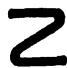
\includegraphics[keepaspectratio]{images/part002_2a386891d62f089ad1c0e080d8072868eea932699f46973e31691c72a41ba0df.jpg}}

``对所有 \(x \in E\) , \(f(x) \leqslant g(x)\) ，并且存在

且不

\[
f (y) <   g (y) ^ {\prime \prime}
\]

\[
" \text { 对   所有 } x \in \mathrm{E}, f (x) <   g (x)".
\]

为了避免混淆，在这种情况下最好不要使用记号 \(f < g\) 。

本小节的定义在不作改动的情况下适用于预序集，只需将全文中的“序”替换为“预序”。

\subsection{递增映射}

定义1. 设E和F为预序集（其中每个集中的预序关系均记为 \(\leqslant\) ）。从E到F的映射f被称为递增的（或保序的），如果关系 \(x \leqslant y\) 蕴含 \(f(x) \leqslant f(y)\) ；如果满足关系 \(x \leqslant y\) 蕴含 \(f(x) \geqslant f(y)\) ，则称其为递减（或反序）映射。从E到F的映射若为递增或递减，则称其为单调的。

当我们将E或F上的一个预序替换为其相反预序时，从E到F的递增映射变为递减映射（反之亦然）。每个常值函数既是递增的又是递减的；该命题的逆命题通常不成立。

例如，若集合E按相等关系排序，则E到自身的恒等映射既是递增的又是递减的，但当E含有多于一个元素时，它并非常值映射（参见习题7）。

定义2. 设E和F是两个有序集。将E映入F的映射f称为严格递增（或严格保序）的，如果关系x \textless{} y 蕴含 \(f(x) < f(y)\) ；如果关系 x \textless{} y 蕴含 \(f(x) > f(y)\) ，则称其为严格递减（或严格反序）的。将E映入F的映射称为严格单调的，如果它要么严格递增，要么严格递减。

示例

\begin{enumerate}
\def\labelenumi{(\arabic{enumi})}
\item
  设 E 为一个集合。映射 \(X \rightarrow E - X\) 是 \(\mathfrak{P}(E)\) （按包含关系排序）到自身的严格递减映射。
\item
  设 E 是一个有序集。对于每个 \(x \in E\) ，设 \(U_x\) 为所有 \(y \in E\) 中使得 \(y \geqslant x\) 的元素所成的集合. 映射 \(x \to U_x\) 是 E 到 \(\mathfrak{P}(E)\) （按包含关系排序）的一个严格递减映射；事实上，关系 \(x \leqslant y\) 等价于 \(U_x \supset U_y\) .
\end{enumerate}

有序集E到有序集F的单调单射是严格单调的；其逆命题通常不成立，因为可能有 \(f(x) = f(y)\) 当关系 \(x \leqslant y\) , \(x \geqslant y\) 均不成立时（参见第12号，命题11）。

一个双射映射 \(f\) （从有序集合 \(\mathbf{E}\) 到有序集合 \(\mathbf{E}'\) 上的双射）是 \(\mathbf{E}\) 到 \(\mathbf{E}'\) 上的一个同构（第3号），当且仅当 \(f\) 与其逆映射两者都是递增的。

如果 I 是一个有序指标集，则一族子集 \((\mathbf{X}_t)_{i \in I}\) 称为集合 E 的递增族，如果 \(\iota \to \mathbf{X}_t\) 是从 I 到 \(\mathfrak{P}(\mathbf{E})\) （按包含关系排序）的递增映射（换言之，如果 \(\iota \leqslant x\) 蕴含 \(\mathbf{X}_t \subset \mathbf{X}_x\) ）。类似地，我们定义递减、严格递增或严格递减的子集族 \((\mathbf{X}_t)_{i \in I}\) 。

命题 2. 设 E, E' 是两个有序集，并设 u: E → E' 与 v: E' → E 是两个递减映射，使得对所有 x ∈ E 和所有 x' ∈ E' 都有 v(u(x)) ≥ x 且 u(v(x')) ≥ x'。则

\[
u \circ v \circ u = u \quad \text{且} \quad v \circ u \circ v = v.
\]

由于关系 \(v(u(x)) \geqslant x\) 蕴含 \((u(v(u(x))) \leqslant u(x)\) ，因为 \(u\) 是递减的；另一方面，我们就有 \(u(v(u(x))) \geqslant u(x)\) ，这可通过将 \(x'\) 换为 \(u(x)\) 代入不等式 \(u(v(x')) \geqslant x'\) 而得。因此第一个等式成立；第二个等式的证明类似。

\subsection{极大元与极小元}

定义 3. 设 E 是一个有序集。元素 \(a \in E\) 称为 E 的极小元（相应地，极大元），如果关系 \(x \leqslant a\) （相应地 \(x \geqslant a\) ）蕴含 \(x = a\) .

E 的每个极小元都是关于相反序的极大元，反之亦然。

示例

\begin{enumerate}
\def\labelenumi{(\arabic{enumi})}
\item
  设 A 是一个集合。在 \(\mathfrak{P}(A)\) （按包含关系排序）中由 A 的非空子集组成的子集里，极小元就是由单个元素组成的子集。
\item
  在集合 \(\Phi(\mathbf{E},\mathbf{F})\) （由 \(\mathbf{E}\) 的子集到 \(\mathbf{F}\) （F 非空）的映射所组成的集合）中，按关系“ \(v\) 是 \(u\) 的延拓”（ \(u\) 与 \(v\) 之间）排序，极大元就是从整个 \(\mathbf{E}\) 到 \(\mathbf{F}\) 的映射。
\end{enumerate}

* (3) 在自然整数集 \textgreater{} 1 中，按 m 与 n 之间的关系“m 整除 n”排序，极小元就是素数。 *

* (4) 实数集没有极大元也没有极小元。 *

\subsection{最大元与最小元}

如果存在一个元素 \(a\) 属于有序集 \(\mathbf{E}\) ，使得 \(a \leqslant x\) 对于所有 \(x \in \mathbf{E}\) 成立，那么 \(a\) 是 \(\mathbf{E}\) 中具有此性质的唯一元素；因为如果还有 \(b \leqslant x\) 对于所有 \(x \in \mathbf{E}\) 成立，那么我们就应有 \(a \leqslant b\) 与 \(b \leqslant a\) ，从而 \(a = b\) .

定义 4. 设 E 是一个有序集。元素 \(a \in E\) 被称为 E 的最小（相应地，最大）元素，如果对所有 \(x \in E\) 我们有 \(a \leqslant x\) （相应地 \(x \leqslant a\) ）.

一个有序集不一定有最大元素，也不一定有最小元素。如果 E 有最小元素 a，则 a 是关于相反序的最大元素。

如果 E 有最小元素 \(a\) ，那么 \(a\) 是 E 的唯一极小元素；因为如果 \(x \in E\) 不同于 \(a\) ，我们就有 \(a < x\) .

示例

\begin{enumerate}
\def\labelenumi{(\arabic{enumi})}
\item
  设 \(\mathfrak{S}\) 为集合 \(\mathfrak{P}(\mathbf{E})\) （集合 \(\mathbf{E}\) 的子集所成的集合）的一个非空子集。如果 \(\mathfrak{S}\) 关于包含关系有最小（相应地，最大）元素A，则A是 \(\mathfrak{S}\) 中这些集合的交集（相应地，并集）。反之，若 \(\mathfrak{S}\) 中这些集合的交集（相应地，并集）属于 \(\mathfrak{S}\) ，则它是 \(\mathfrak{S}\) 的最小（相应地，最大）元素。
\item
  特别是， \(\varnothing\) 是最小元素，而E是最大元素，均在 \(\mathfrak{P}(E)\) 中。在集合 \(\Phi(E, F)\) （从E的子集到F的映射所成的集合）中，按映射的延拓排序（第1号，例3），空映射是最小元素，且除非F由单一元素组成，否则不存在最大元素。对角线 \(\Delta\) ，即 \(E \times E\) 的对角线，是 E 上等价关系的图所成集合（或 E 上的预序所成集合）的最小元素。
\end{enumerate}

命题 3. 设 E 是一个有序集，并设 E' 是 E 与一个集合 \{a\} （由单个元素组成）的不交并。那么存在唯一的E'上的序，它诱导出E上给定的序，并且使得a是E'的最大元素。

事实上，如果 G 是 E 上序关系的图，那么 \(E'\) 上满足命题条件的序关系之图，必为并集 \(G'\)，即 G 与所有二元组 \((x, a)\) 所成集合的并，其中 \(x \in E'\)；反之，显然 \(G'\) 是 \(E'\) 上一个满足给定条件的序关系之图。¶ 称有序集 \(E'\) 是由 E 添加一个最大元 a 得到的（参见练习 3）。

预序集 E 的子集 A 称为 E 的共尾子集（相应地，共始子集），如果对每个 \(x \in E\) ，存在 \(y \in A\) 使得 \(x \leqslant y\) （相应地 \(y \leqslant x\) ）。说有序集 E 有最大元（相应地，最小元）因此意味着 E 有一个由单个元素组成的共尾（相应地，共始）子集。

\subsection{上界与下界}

定义5. 设E是一个预序集，且X是E的一个子集。任一元素 \(x \in \mathbf{E}\) ，若它使得 \(x \leqslant y\) （相应地 \(x \geqslant y\) ）对所有 \(y \in \mathbf{X}\) 成立，则被称为X在E中的下界（相应地，上界）。

X 的每个上界都是 X 关于相反序的下界，反之亦然。

如果 \(x\) 是 \(\mathbf{X}\) 的一个下界，则每个元素 \(z \leqslant x\) 也是 \(\mathbf{X}\) 的一个下界。 \(\mathbf{X}\) 的一个下界也是 \(\mathbf{X}\) 的每个子集的下界。有序集 \(\mathbf{X}\) 有最小元当且仅当存在 \(\mathbf{X}\) 的一个下界，它属于 \(\mathbf{X}\) .

预序集E的子集X的下界集合可能为空：当X=E且E是没有最小元素的有序集时，就是这种情况。

E的子集X，如果其下界（相应地，上界）集合非空，则称X下有界（相应地，上有界）。既下有界又上有界的子集称为有界。如果X下有界（相应地，上有界，有界），则X的每个子集也是如此。

由单个元素组成的每个子集都是有界的。但由两个元素组成的子集不一定上有界或下有界（第10号）。

设E是一个预序集，并设f是从任意集合A到E的一个映射。映射f（按语言的滥用）被称为下有界（相应地，上有界，有界），如果集合 \(f(\mathbf{A})\) 在E中是下有界（相应地，上有界，有界）的。

\subsection{最小上界与最大下界}

定义6. 设E是一个有序集，并设X是E的一个子集。E中的一个元素称为X在E中的最大下界或下确界（相应地，最小上界或上确界），如果它是X在E中的下界（相应地，上界）集合的最大（相应地，最小）元素。

给定有序集E的一个子集X，X在E中的最小上界（相应地，最大下界），当它存在时，记为

\[
\sup _ {\mathbf {E}} \mathbf {X} (\text { 分别   inf } _ {\mathbf {E}} \mathbf {X})
\]

或记为sup X（相应地，inf X），如果没有歧义的话。一个集合 \(\{x, y\}\) 的两个元素的最小上界（相应地，最大下界），当它存在时，记为sup \((x, y)\) （相应地，inf \((x, y)\) )。类似地，对于三个元素集合的上确界和下确界，等等。如果E的子集X有最大元素a，则a是X在E中的上确界。

如果X在E中有最大下界 \(a\) ，则 \(a\) 是关于E上相反序的X的最小上界。因此，在接下来的内容中，我们大多可以仅限于考虑最小上界的性质。

\minorheading{示例}

\begin{enumerate}
\def\labelenumi{(\arabic{enumi})}
\item
  在一个有序集合E中，空集 \(\phi\) 的上界集合显然就是E本身；因此 \(\phi\) 在E中有上确界当且仅当E有最小元素，此时该最小元素即为 \(\phi\) 的最小上界。
\item
  在集合 \(\mathfrak{P}(\mathbf{E})\) （集合 \(\mathbf{E}\) 的子集所成的集合，按包含关系排序）中，每个子集 \(\mathfrak{S}\) （ \(\mathfrak{P}(\mathbf{E})\) 的子集）都具有最小上界，即 \(\mathfrak{S}\) 中这些集合的并集，以及一个最大下界，即 \(\mathfrak{S}\) 中这些集合的交集。
\item
  设 E、F 为两个集合，并设 \(\Theta\) 是 \(\Phi(\mathbf{E}, \mathbf{F})\) 的子集，其中映射是从 E 的子集到 F 的映射族，按映射的延拓来排序（第 1 号，例 3）。对每个 \(u \in \Phi(\mathbf{E}, \mathbf{F})\) ，设 \(\mathbf{D}(u)\) 为 u 的定义域。一族属于 \(\Phi(\mathbf{E}, \mathbf{F})\) 的映射存在公共延拓的条件（第二章，§ 4，第 6 号，命题 7）表明 \(\Theta\) 在 \(\Phi(\mathbf{E}, \mathbf{F})\) 中有最小上界，当且仅当对于每一对元素 \((u, v)\) （ \(\Theta\) 的元素）我们有 \(u(x) = v(x)\) ，每当 \(x \in \mathbf{D}(u) \cap \mathbf{D}(v)\) 时。
\end{enumerate}

一个映射 \(f\) （从集合 \(A\) 到有序集 \(E\) 中的映射）称为具有最小上界，如果像 \(f(A)\) 在 \(E\) 中有最小上界；这个界随后称为 \(f\) 的最小上界，并记作 \(\sup_{x \in A} f(x)\) 。对于最大下界也有类似的定义。

特别地，如果 E 的子集 A 在 E 中具有最小上界，则该界是 A 到 E 的典范单射的最小上界，因此可以写成 sup x。

命题 4. 设 E 是一个有序集，A 是 E 的一个子集，且 A 在 E 中既有最大下界又有最小上界。若 A ≠ ∅，则 inf A ≤ sup A；若 A = ∅，则 sup A 是 E 的最小元素，inf A 是 E 的最大元素。

这直接由定义得出。

命题 5. 设 E 是一个有序集，A、B 是 E 的两个子集，且每个子集在 E 中都有最小上界（相应地，最大下界）。若 A ⊂ B，则 sup A ≤ sup B（相应地，inf A ≥ inf B）。

推论。设 \((x_{t})_{i\in I}\) 是某个有序集 \(E\) 的一个元素族，该族在 \(E\) 中有最小上界。如果 \(J\) 是 \(I\) 的一个子集，使得该族 \((x_{t})_{i\in J}\) 在 \(E\) 中有最小上界，我们就有 \(\sup_{i\in J}x_i\leqslant \sup_{i\in I}x_i\) .

命题6. 设 \((x_{i})_{i\in I}, (y_{i})_{i\in I}\) 是同一个指标集 I 索引的有序集 E 的两个元素族，并且满足 \(x_{i} \leqslant y_{i}\) （对于所有 \(i\in I\) ）。若两个族在 E 中都有最小上界，则 \(\sup_{i\in I} x_{i} \leqslant \sup_{i\in I} y_{i}\) .

因为 \(a = \sup_{i \in I} y_i\) 是由各 \(y_i\) 组成的集合的一个上界，所以 \(x_i \leqslant y_i \leqslant a\) 对所有 \(i \in I\) 都成立，从而 \(\sup_{i \in I} x_i \leqslant a\) .

命题7. 设 \((x_{t})_{t\in I}\) 是某个有序集 \(E\) 的元素族，并且设 \((J_{\lambda})_{\lambda \in I}\) 是指标集 \(I\) 的一个覆盖。假设每个子族 \((x_{t})_{t\in J_{\lambda}}\) 在 \(E\) 中有最小上界。对于该族 \((x_{t})_{t\in I}\) 在 \(E\) 中具有最小上界，其充分必要条件是该族 \(\left(\sup_{t\in J_{\lambda}}x_{t}\right)_{\lambda \in L}\) 在 \(E\) 中具有最小上界，此时我们有

\[
\sup _ {i \in I} x _ {i} = \sup _ {\lambda \in L} \left(\sup _ {i \in J _ {\lambda}} x _ {i}\right).\tag{1}
\]

令 \(b_{\lambda} = \sup_{i \in J_{\lambda}} x_i\) 。假设 \((x_i)_{i \in I}\) 具有最小上界 \(a\) 。则 \(a \geqslant b_{\lambda}\) （对于每一个 \(\lambda \in L\) ）（命题5的推论）。另一方面，如果 \(c \geqslant b_{\lambda}\) 对于每一个 \(\lambda \in L\) ，那么我们有 \(c \geqslant x_i\) 对于每一个 \(i \in I\) ，因为 \((J_{\lambda})_{\lambda \in L}\) 是 \(I\) 的一个覆盖；因此 \(c \geqslant a\) ，这证明了

\[
a = \sup _ {\lambda \in L} b _ {\lambda}.
\]

反之，假设该族 \((b_{\lambda})_{\lambda \in \mathbf{L}}\) 具有最小上界 \(a'\) 。则 \(a' \geqslant x_{i}\) 对于所有 \(i \in I\) 。另一方面，如果 \(c' \geqslant x_{i}\) 对于所有 \(i \in I\) ，那么我们特别有

\[
c ^ {\prime} \geqslant \sup _ {i \in J _ {\lambda}} x _ {i} = b _ {\lambda}
\]

对于每一个 \(\lambda \in \mathbf{L}\) ，因此 \(c' \geqslant a'\) ，从而

\[
a ^ {\prime} = \sup _ {i \in I} x _ {i}.
\]

推论。设 \((x_{\lambda \mu})_{(\lambda, \mu) \in \mathbf{L} \times \mathbf{M}}\) 是某个有序集合 \(\mathbf{E}\) 的一个“双重”元素族，使得对于每一个 \(\mu \in \mathbf{M}\) ，族 \((x_{\lambda \mu})_{\lambda \in \mathbf{L}}\) 在 \(\mathbf{E}\) 中有最小上界。该族 \((x_{\lambda \mu})_{(\lambda, \mu) \in \mathbf{L} \times \mathbf{M}}\) 在 \(\mathbf{E}\) 中具有最小上界的充分必要条件是，族 \(\left(\sup_{\lambda \in \mathbf{L}} x_{\lambda \mu}\right)_{\mu \in \mathbf{M}}\) 在 E 中具有最小

上界，此时我们有

\[
\sup _ {(\lambda , \mu) \in L \times M} x _ {\lambda \mu} = \sup _ {\mu \in M} \left(\sup _ {\lambda \in L} x _ {\lambda \mu}\right).\tag{2}
\]

命题8. 设 \((\mathbf{E}_t)_{t \in I}\) 是一族有序集。设 A 是乘积有序集 \(\mathbf{E} = \prod_{t \in I} \mathbf{E}_t\) 的一个子集，并且设 \(\mathbf{A}_t = \operatorname{pr}_t \mathbf{A}\) （对于每一个 \(t \in I\) ）。要使 A 在 \(\mathbf{E}\) 中有最小上界，必要且充分的条件是：对每个 \(t \in I\) , \(\mathbf{A}_t\) 在 \(\mathbf{E}_t\) 中有最小上界，此时我们有

\[
\sup A = (\sup A _ {t}) _ {t \in I} = \left(\sup _ {x \in A} \operatorname{pr} _ {t} x\right) _ {t \in I}.
\]

假设对于每一个 \(t \in I\) , \(A_t\) 具有最小上界 \(b_t\) （在 \(E_t\) 中）. 要说 \(c = (c_t)\) 是 \(A\) 的一个上界，那就意味着 \(c_t \geqslant b_t\) 对于每一个 \(t \in I\) 成立，因此 \((b_t)_{t \in I}\) 是 \(A\) 的一个上界。相反，假设 \(A\) 具有最小上界 \(a = (a_t)_{t \in I}\) ；对于每个 \(x \in I\) , \(a_x\) 是 \(A_x\) 的一个上界，因为如果 \(x_x \in A_x\) , 就存在 \(x \in A\) 使得 \(pr_x x = x_x\) ，这由 \(A_x\) 的定义可得；另一方面，如果 \(a_x'\) 是 \(A_x\) 在 \(E_x\) 中的一个上界，那么元素 \(c' = (c_t')_{t \in I}\) （对于它）

\[
c _ {i} ^ {\prime} = a _ {i} \quad \text { 对 } \quad i \neq x \quad \text { 且 } \quad c _ {x} ^ {\prime} = a _ {x} ^ {\prime}
\]

是A的一个上界；于是 \(c' \geqslant a\) ，因而 \(a_{x}' \geqslant a_{z}\) ；因此 \(a_{x}\) 是 \(A_{x}\) 在 \(E_{x}\) 中的最小上界.

\pandocbounded{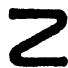
\includegraphics[keepaspectratio]{images/part002_f683a60c9eaa907b29b9c0e21fae4a1da7b4dd647e1d1a410962ae330fdaf4f4.jpg}}

设F是有序集E的一个子集，并设A是F的一个子集。可能发生两个元素 \(\sup_{E} A\) , \(\sup_{F} A\)

示例

中的一个存在而另一个不存在，或者两者都存在但不相等。* (1) 在实数有序集 \(\mathbf{E} = \mathbf{R}\) （实数集）中，考虑有理数子集 \(\mathbf{F} = \mathbf{Q}\) 以及有理数集 \(\mathbf{A} \subset \mathbf{F}\) ，即满足 \(< \sqrt{2}\) 的有理数所成的集； \(\sup_{\mathbf{E}} \mathbf{A}\) 存在但 \(\sup_{\mathbf{F}} \mathbf{A}\) 不存在。

\begin{enumerate}
\def\labelenumi{(\arabic{enumi})}
\setcounter{enumi}{1}
\item
  在例1的记号中，设G为A与集合 \(\{2\}\) 的并集；那么 \(G \subset F\) ，并且 \(\sup_{G} A\) 存在，但 \(\sup_{F} A\) 不存在。
\item
  使用相同的记号， \(\sup_{\mathbf{E}} \mathbf{A} = \sqrt{2}\) , \(\sup_{\mathbf{G}} \mathbf{A} = 2\) . *
\end{enumerate}

然而，我们有以下结果：

命题9. 设E是一个有序集，F是E的一个子集，A是F的一个子集。如果 \(\sup_{\mathbf{E}}\mathbf{A}\) 与 \(\sup_{\mathbf{F}}\mathbf{A}\) 都存在，我们有 \(\sup_{\mathbf{E}}\mathbf{A} \leqslant \sup_{\mathbf{F}}\mathbf{A}\) 。如果 \(\sup_{\mathbf{E}}\mathbf{A}\) 存在且属于F，则 \(\sup_{\mathbf{F}}\mathbf{A}\) 存在且等于 \(\sup_{\mathbf{E}}\mathbf{A}\) .

第一个断言由以下事实得出：A在F中的上界集合M包含于A在E中的上界集合N，以及命题5。另一方面，如果N的最小元属于F，则它属于M，并且显然是M的最小元；这证明了第二个断言。

\subsection{有向集}

定义7. 一个预序集E被称为右有向的（相应地，左有向的），如果E的任意两个元素构成的子集都有上界（相应地，有下界）。

我们常常用“关于关系 \(\leqslant\) 有向”来代替“右有向”，以及当预序关系用其他符号表示时的类似表达式。例如，若S是集合A的子集族，我们说S关于关系 \(\subset\) （相应地 \(\supset\) ）是定向的，如果对于每个由S中两个元素组成的子集 \(\{X, Y\}\) ，存在 \(Z \in S\) 使得 \(X \subset Z\) 并且 \(Y \subset Z\) （相应地 \(X \supset Z\) 并且 \(Y \supset Z\) ）。

示例

\begin{enumerate}
\def\labelenumi{(\arabic{enumi})}
\tightlist
\item
  具有最大元素的有序集是右定向的。
\end{enumerate}

* (2) 在拓扑空间中，一个点的邻域基关于关系 \(\supset\) 是定向的。

\begin{enumerate}
\def\labelenumi{(\arabic{enumi})}
\setcounter{enumi}{2}
\tightlist
\item
  任意模的有限型子模所成的集合关于关系 \(\subset\cdot_{*}\) 是定向的。
\end{enumerate}

命题10. 在右有向有序集E中，一个极大元 \(a\) 是E的最大元。

对于每一个 \(x \in \mathbf{E}\) ，由假设存在 \(y \in \mathbf{E}\) 使得 \(x \leqslant y\) 并且 \(a \leqslant y\) ；由于 \(a\) 是极大元，故 \(y = a\) .

右有向预序集关于相反序是左有向的。右有向集的任何乘积都是右有向的。另一方面，右有向集的子集不一定是右有向的。然而，右有向集E的共尾子集F总是右有向的；对于给定的 \(x, y \in \mathbf{F}\) ，存在 \(z \in \mathbf{E}\) 使得 \(x \leqslant z\) 并且 \(y \leqslant z\) ，然后再取 \(t \in \mathbf{F}\) 使得 \(z \leqslant t\) .

\subsection{格}

定义8. 一个有序集E被称为格，如果E的每个由两个元素组成的子集在E中都有最小上界和最大下界。

格的每个乘积都是格；这由有序集乘积中最小上界存在的条件（第9号，命题8）得出。集合A的子集所构成的集合，按包含关系排序，是一个格，因为A的两个子集的并集和交集仍然是A的子集。

\minorheading{示例}

* (1) 整数集 \(\geqslant 1\) ，按 \(m\) 与 \(n\) 之间的关系“ \(m\) 整除 \(n\) ”排序，是一个格； \(\{m, n\}\) 的最小上界是 \(m\) 与 \(n\) 的最小公倍数，而最大下界是它们的最大公因数。

\begin{enumerate}
\def\labelenumi{(\arabic{enumi})}
\setcounter{enumi}{1}
\item
  群G的子群集合，按包含关系排序，构成一个格。
\item
  集合A上的所有拓扑所成的集合，按 \(\mathfrak{G}\) 与 \(\mathfrak{G}'\) 之间的关系“ \(\mathfrak{G}\) 比 \(\mathfrak{G}'\) 更粗”排序，是一个格。（一般拓扑学，第一章，§2）。
\item
  集合 \(\mathcal{F}(\mathbf{I},\mathbf{R})\) ，即定义在区间 \(\mathbf{I}\) （ \(\mathbf{R}\) 中的区间）上的所有实值函数所成的集合，关于序关系 \(f\leqslant g\) （第4号）是一个格，并且作为这样的格同构于乘积 \(\mathbf{R}^{\mathrm{I}}\) . *
\end{enumerate}

注记。一个格显然既是左有向的又是右有向的。但一个既是左有向又是右有向的有序集不一定是格。* 后者的一个例子是映射 \(x \to p(x)\) （从 \(\mathbf{R}\) 到其自身的映射）所成的集合，其中 \(p\) 是 \(\mathbf{R}[\mathbf{X}]\) 中的多项式，该集合按关系 \(p \leqslant q\) 排序（第4号）。*

\subsection{全序集}

定义9. 两个元素 \(x, y\) （预序集 \(E\) 的元素）称为可比较的，如果关系“ \(x \leqslant y\) 或 \(y \leqslant x\) ”为真。一个集合 \(E\) 称为全序的，如果它是有序的，并且 \(E\) 的任意两个元素是可比较的。 \(E\) 上的序则被称为全序，相应的序关系称为全序关系。

如果 \(x\) 与 \(y\) 为全序集的元素，则要么 \(x = y\) ，要么 \(x < y\) ，要么 \(x > y\) ； \(x \leqslant y\) 的否定因而是 \(x > y\) .

 \(\mathbf{E}\) 上的一个序关系是全序的，当且仅当其图 \(\mathbf{G}\) 满足关系 \(\mathbf{G} \cup \overline{\mathbf{G}} = \mathbf{E} \times \mathbf{E}\) 以及关系 \(\mathbf{G} \circ \mathbf{G} = \mathbf{G}\) 和 \(\mathbf{G} \cap \overline{\mathbf{G}} = \Delta\) .

示例

\begin{enumerate}
\def\labelenumi{(\arabic{enumi})}
\item
  全序集的每个子集在诱导序下都是全序的。
\item
  设 E 为任意有序集。E 的空子集是全序的，E 的每个单元素子集也是全序的。
\end{enumerate}

* (3) 集合 \(\mathbf{R}\) （实数集）是全序的。*

\begin{enumerate}
\def\labelenumi{(\arabic{enumi})}
\setcounter{enumi}{3}
\tightlist
\item
  若 A 是至少含有两个不同元素的集合，则集合 \(\mathfrak{P}(A)\) （按包含关系排序）不是全序的，因为若 \(x \neq y\) ，则子集 \(\{x\}\) 与 \(\{y\}\) 不可比较。
\end{enumerate}

全序集在相反序下也是全序的；它是一个格，因而更是左有向且右有向的。

命题 11. 每个严格单调映射 \(f\) （从全序集 \(\mathbf{E}\) 到有序集 \(\mathbf{F}\) 的映射）都是单射。若 \(f\) 严格递增，则 \(f\) 是 \(\mathbf{E}\) 到 \(f(\mathbf{E})\) 上的一个同构.

因为 \(x \neq y\) 蕴含 \(x < y\) 或 \(x > y\) ；因此

\[
f (x) <   f (y) \quad \text { 或 } \quad f (x) > f (y),
\]

使得 \(f(x) \neq f(y)\) 在任一情形下均如此。还需证明若 \(f\) 严格递增，则 \(f(x) \leqslant f(y)\) 蕴含 \(x \leqslant y\) ；否则，我们应有 \(x > y\) ，从而 \(f(x) > f(y)\) .

命题 12. 设 E 为全序集，X 为 E 的子集。对于 E 中的元素 b 而言，b 是 X 在 E 中的最小上界，当且仅当 (1) b 是 X 的上界，(2) 对每个 \(c \in E\) （使得 c \textless{} b ），存在 \(x \in X\) 使得 \(c < x \leqslant b\) .

第二个条件说明没有元素 c \textless{} b 是 X 的上界，即 b 是 X 的上界集合 M 的极小元素；但由于 M 是全序的（第 10 号，命题 10），这与 b 是 M 的最小元素是等价的。

\subsection{区间}

设 E 是一个有序集，并设 a, b 是 E 的两个元素，使得 \(a \leqslant b\) 。E 中由满足 \(a \leqslant x \leqslant b\) 的元素 x 组成的子集称为以 a 为左端点、b 为右端点的闭区间，并记为 {[}a, b{]}。所有满足 \(x \in E\) 且 \(a \leqslant x < b\) （相应地 \(a < x \leqslant b\) ）的 x 所成的集合称为以 a 和 b 为端点的右半开（相应地，左半开）区间，并记为 {[}a, b{[} （相应地 {]}a, b{]}）。所有满足 \(x \in E\) 且 a \textless{} x \textless{} b 的 x 所成的集合称为以 a 和 b 为端点的开区间，并记为 {]}a, b{[}。注意，闭区间永远非空；

另一方面，闭区间 \([a, a]\) 是集合 \(\{a\}\) ；而区间 \([a, a[, ]a, a], ]a, a[\) 都是空的；且开区间 \(]a, b[\) 即使当 \(a < b\) 时也可能为空。

设 \(a\) 为 \(E\) 的一个元素。所有满足 \(x \in E\) 且 \(x \leqslant a\) （相应地 \(x < a\) ）的 x 所成的集合称为左无界、右端点为 \(a\) 的闭（相应地，开）区间，并记作 \(] \leftarrow, a]\) （相应地 \(] \leftarrow, a[\) ）；同样地，所有满足 \(x \in E\) 且 \(x \geqslant a\) （相应地 \(x > a\) ）的 x 所成的集合称为左端点为 \(a\) 、右无界的闭（相应地，开）区间，并记为 \([a, \leftarrow[\) （相应地 \(]a, \leftarrow[\) ）。最后， \(E\) 本身可以看作左、右均无界的开区间，记为 \(] \leftarrow, \rightarrow [.\)

命题 13. 在一个格中，两个区间的交集是一个区间。例如考虑两个闭区间 \([a, b]\) 与 \([c, d]\) 的交集，并设 \(\alpha = \sup (a, c)\) , \(\beta = \inf (b, d)\) 。如果 \(a \leqslant x \leqslant b\) 与 \(c \leqslant x \leqslant d\) 两者都成立，那么我们有 \(\alpha \leqslant x \leqslant \beta\) ，且反之亦然；如果 \(\alpha \not\leqslant \beta\) ，则 \([a, b]\) 与 \([c, d]\) 的交集为空；如果 \(\alpha \leqslant \beta\) ，则此交集为 \([\alpha, \beta]\) 。其余情形下的证明留给读者完成。

\section{良序集}

\subsection{良序集的段}

一个关系 \(R\{x, y\}\) 称为 x 与 y 之间的良序关系，如果 R 是 x 与 y 之间的一个序关系，并且对于每个非空集合 E，若 \(R\{x, y\}\) 在 E 上诱导一个序关系（即满足 \(x \in E\) 蕴含 \(R\{x, x\}\) ；参见§1，第1号），则按此关系有序的 E 有一个最小元素。

一个由序 \(\Gamma\) 所排序的集合 E 被称为良序的，如果关系 \(y \in \Gamma\langle x \rangle\) 是 x 与 y 之间的良序关系； \(\Gamma\) 则称为 E 上的一个良序。以下定义与此等价：

定义1. 若集合E是有序的，且E的每个非空子集都有最小元素，则称E为良序的。

一个良序集 E 是全序的，因为 E 的每个子集 \(\{x, y\}\) 都有一个最小元素。E 的每个在 E 中有上界的子集 A 在 E 中都有一个最小上界。

\minorheading{示例}

\begin{enumerate}
\def\labelenumi{(\arabic{enumi})}
\item
  设 \(\mathbf{E} = \{\alpha, \beta\}\) 是一个元素互不相同的集合。容易验证， \(\{(\alpha, \alpha), (\beta, \beta), (\alpha, \beta)\}\) 这个 \(\mathbf{E} \times \mathbf{E}\) 的子集是 \(\mathbf{E}\) 上一个良序的图.
\item
  良序集的每个子集（特别是空子集）在诱导序下都是良序的。
\end{enumerate}

* (3) 存在非良序的全序集等价于无穷公理（§ 4，第 4 号，命题 3 的推论 1，以及练习 3）。

\begin{enumerate}
\def\labelenumi{(\arabic{enumi})}
\setcounter{enumi}{3}
\item
  如果 \(\Gamma\) 是 \(E\) 上的一个良序，则与 \(\Gamma\) 相反的序是 \(E\) 上的良序仅当 \(E\) 是有限的（ \(\S 4\) ，练习3）。*
\item
  设 E 是一个良序集。集合 \(E_{1}\) 通过向 E 添加一个最大元素 b（§1，第 7 号）而得到，是良序的，因为若 H 是 \(E_{1}\) 的任意非空子集且异于 \(\{b\}\) ，则 \(H \cap E\) 的最小元素也是 H 的最小元素。
\end{enumerate}

注记。 * 作为无穷公理（§6，第1号）的一个推论，存在没有最大元素的良序集，例如自然整数集 N。 *

定义2. 在有序集 E 中，E 的一个子集，若关系 \(x \in S\) , \(y \in E\) ，以及 \(y \leqslant x\) 蕴含 \(y \in S\) ，则称为E的一个段。

显然，E 的段的任意交和并都是 E 的一个段。若 S 是 E 的一个段，则 S 的每个段也是 E 的一个段。集合 E 本身和空集都是 E 的段。

命题1. 在一个良序集E中，E的每个不同于E本身的段都是一个区间 {]}←，a{[}，其中 a ∈ E。

设 S 为 E 的一个段，且 \(S \neq E\) 。由于 E --- S 非空，它有一个最小元素 a。根据定义 2，关系 \(x \geqslant a\) 蕴含 \(x \notin S\) ；否则就会有 \(a \in S\) ，这是矛盾的。因此 E --- S 是区间 \([a, \rightarrow[, \text{ 且 } S \text{ 是区间}] \leftarrow, a[\) .

对于每个元素 \(x\) （属于全序集 \(\mathbf{E}\) ），区间 \(] \leftarrow, x[\) 称为以 \(x\) 为端点的段，并记作 \(\mathbf{S}_x\) .

注意，若E是良序的且非空， \(S_{x}\) 有一个最小元素 \(\alpha\) ，因此它也是区间 \([\alpha, x[\) .

设E为全序集。诸 \(S_{x}\) （其中x遍历E）的并集A，当E无最大元时即为E；若E有最大元b，则 \(A = E - \{b\}\) .

命题2. 集合 \(\mathbf{E}^*\) （良序集 \(\mathbf{E}\) 的段所成的集合）按包含关系是良序的。映射 \(x \to S_x\) 是良序集 \(\mathbf{E}\) 到 \(\mathbf{E}\) 的异于 \(\mathbf{E}\) 本身的段所成集合上的同构。

显然，如果 \(x \in \mathbf{E}\) 并且 \(y \in \mathbf{E}\) ，关系 \(x \leqslant y\) 蕴含 \(\mathrm{S}_x \subset \mathrm{S}_y\) ，以及 \(x < y\) 蕴含 \(\mathrm{S}_x \neq \mathrm{S}_y\) ；因此映射 \(x \to \mathrm{S}_x\) 是 \(\mathbf{E}\) 到集合 \(\mathrm{S}(\mathbf{E})\) （ \(\mathbf{E}\) 的异于 \(\mathbf{E}\) 本身的段所成的集合）上的同构（§1，第12号，命题11），因此 \(\mathrm{S}(\mathbf{E})\) 是良序的。此外， \(\mathbf{E}^*\) 同构于由 \(\mathrm{S}(\mathbf{E})\) 通过添加一个最大元所得到的良序集。

命题3. 设 \((\mathbf{X}_{\iota})_{\iota \in \mathbf{I}}\) 是一族良序集，使得对于每一对指标 \((\iota, \varkappa)\) ，集合 \(\mathbf{X}_{\iota}, \mathbf{X}_{\varkappa}\) 中的一个是另一个的段。那么在集合 \(\mathbf{E} = \bigcup_{\iota \in \mathbf{I}} \mathbf{X}_{\iota}\) 上存在唯一的序关系，它在每一个 \(\mathbf{X}_{\iota}\) 上诱导出给定的序关系。在此序下， \(\mathbf{E}\) 是良序集。 \(X_{t}\) 的每一段是E的一个段；对于每个 \(x \in X_{t}\) ， \(X_{t}\) 中以x为端点的段等于E中以x为端点的段；并且E的每个段要么是E本身，要么是其中一个 \(X_{t}\) 的段。

第一个断言是以下一般引理的推论：

引理1. 设 \((\mathbf{X}_{\alpha})_{\alpha \in \Lambda}\) 为一个有序集族，它关于关系 \(c\) 是定向的（换言之，即对于每一对索引 \(\alpha, \beta\) 存在一个指标 \(\gamma\) 使得 \(\mathbf{X}_{\alpha} \subset \mathbf{X}_{\gamma}\) 并且 \(\mathbf{X}_{\beta} \subset \mathbf{X}_{\gamma}\) ）。假设对于每一对指标 \((\alpha, \beta)\) ，若 \(\mathbf{X}_{\alpha} \subset \mathbf{X}_{\beta}\) ，则 \(\mathbf{X}_{\alpha}\) 上由 \(\mathbf{X}_{\beta}\) 的序诱导的序与 \(\mathbf{X}_{\alpha}\) 上给定的序相同。在这些条件下，集合 \(\mathbf{E} = \bigcup_{\alpha \in \Lambda} \mathbf{X}_{\alpha}\) 上存在唯一的序关系，该序关系在每个子集 \(\mathbf{X}_{\alpha}\) 上诱导出给定的序关系。

设 \(G_{\alpha}\) 为给定序关系在 \(X_{\alpha}\) 上的图。若G是E上一个序的图，且该序在每一 \(X_{\alpha}\) 上诱导的序就是以 \(G_{\alpha}\) 为图的那个序，那么我们必须有 \(G_{\alpha} \subset G\) 对于每一个 \(\alpha \in A\) ；因此 G 包含 \(\bigcup_{\alpha \in A} G_{\alpha}\) 。另一方面，对于 E 的每一对元素 \((x, y)\) ，根据假设存在一个指标 \(\alpha \in A\) 使得 \(x \in X_{\alpha}\) 并且 \(y \in X_{\alpha}\) ；若 \((x, y) \in G\) ，我们有 \((x, y) \in G_{\alpha}\) ，因此 \(G \subset \bigcup_{\alpha \in A} G_{\alpha}\) 。因此，如果 E 上所需的序存在，则其图必然是 \(G = \bigcup_{\alpha \in A} G_{\alpha}\) 。剩下的只需证明该集合满足引理的条件。由于 \(G_{\beta} \cap (X_{\alpha} \times X_{\alpha}) = G_{\alpha}\) 若 \(X_{\alpha} \subset X_{\beta}\) ，我们有 \(G \cap (X_{\alpha} \times X_{\alpha}) = G_{\alpha}\) 对于所有 \(\alpha \in A\) ；另一方面，由假设可知，E 中任意三个元素 \(x, y, z\) 属于同一个 \(X_{\alpha}\) 。因此 \((x, y) \in G\) 是 E 上的一个序关系，引理得证。

我们现在开始证明命题3。首先，我们来证明每一个 \(\mathbf{X}_{\iota}\) 是 E 的一段。事实上，如果 \(x \in \mathbf{X}_{\iota}, y \in \mathbf{E}\) ，以及 \(y \leqslant x\) ，存在一个指标 \(x\) 使得 \(\mathbf{X}_{\iota} \subset \mathbf{X}_{x}\) 并且 \(y \in \mathbf{X}_{x}\) ；由于根据假设 \(\mathbf{X}_{\iota}\) 是 \(\mathbf{X}_{x}\) 的一段，我们有 \(y \in \mathbf{X}_{\iota}\) ，这证明了该断言。同样的推理证明，对于每一个 \(x \in \mathbf{X}_{\iota}\) ，以 \(x\) 为端点的段在 \(\mathbf{X}_{\iota}\) 中与E中的区间 {]}←, \(x[\) 相同。接下来让我们证明E是良序的。如果H是E的一个非空子集，则存在一个指标 \(\iota \in I\) 使得 \(\mathrm{H} \cap \mathrm{X}_{\iota} \neq \emptyset\) ；若 \(a\) 是 \(\mathrm{H} \cap \mathrm{X}_{\iota}\) 在 \(\mathbf{X}_{\iota}\) 中的最小元素，那么 \(a\) 也是 H 在 E 中的最小元素。也就是说，如果 \(x \in H\) ，存在一个指标 \(x \in I\) 使得 \(\mathbf{X}_{\iota} \subset \mathbf{X}_{x}\) 并且 \(x \in \mathbf{X}_{x}\) ；我们不可能有 \(x < a\) ，因为区间 {]}←, \(a[\) 包含于 \(\mathbf{X}_{\iota}\) ，因此我们有 \(x \geqslant a\) ，因为 \(\mathbf{X}_{x}\) 是全序的。

最后，我们必须证明E的一个异于E本身的段是其中一个 \(X_{t}\) 的段；这是前述论证的直接结果，因为这样的段具有形式 \(]\leftarrow\) , \(x[\text{(命题1)}\) ，并且由于x属于某个 \(X_{t}\) .

\subsection{超限归纳原理}

引理2. 设E是一个良序集，S是E的一些段构成的集合，且满足以下性质：(1) 属于S的段的任意并仍属于S；(2) 若 \(S_{x} \in S\) ，那么 \(S_{x} \cup \{x\} \in S\) 。则E的每一个段都属于S。

假设E中存在不属于S的段，并设S为其中最小的段（第1号，命题2）。若S没有最大元素，则S是S中不同于S本身的各段的并集，且根据S的定义，这些段都属于S；因此 \(S \in S\) ，这是荒谬的。另一方面，若S有最大元素a，则 \(S = S_{a} \cup \{a\}\) ，且由于 \(S_{a}\) 是 S 的一个不同于 S 的段，我们有 \(S_{a} \in S\) ；但随后也有 \(S \in S\) ，这同样是荒谬的。

为方便起见，我们将置身于一个理论 \(\mathfrak{G}\) 中，在其中 \(\mathbf{E}\) 是一个被写作 \(x \leqslant y\) 的关系良序化的集合。于是我们有以下判据：

C59.（超限归纳原理）。设 \(\mathbf{R}\{x\}\) 是 \(\mathfrak{G}\) 中的一个关系 ( \(x\) 不是 \(\mathfrak{G}\) 的常数 )，使得关系式

\[
(x \in \mathrm{E} \text { 且 } (\forall y) ((y \in \mathrm{E} \text { 且 } y <   x) \Longrightarrow \mathrm{R} \{\left. y \right\})) \Longrightarrow \mathrm{R} \{x \}
\]

在 \(\mathfrak{G}\) 中是定理。在这些条件下，关系 \((x\in \mathbf{E})\Rightarrow \mathbb{R}\{x\}\) 在 \(\mathfrak{G}\) 中是定理。

设 \(\mathfrak{S}\) 是 E 中满足 \((y\in S)\Longrightarrow R\{y\}\) 的段 S 所成的集合。显然，属于 \(\mathfrak{S}\) 的段的每个并集也属于 \(\mathfrak{S}\) 。另一方面，如果 \(S_x\in \mathfrak{S}\) ，由假设我们有 \(R\{x\}\) ；因此 \((y\in S_x\cup \{y\})\Longrightarrow R\{y\}\) 通过分情形讨论的方法。因此（引理2） \(E\in \mathfrak{S}\) ，这证明了该判据。

在C59的应用中，关系

\[
x \in \mathrm{E} \text {   且   } (\forall y) ((y \in \mathrm{E} \text {   且   } y <   x) \Longrightarrow \mathrm{R} \{y \})
\]

通常被称为“归纳假设”。

在以下内容中，对于每一个映射 \(g\) ：它把段 \(S\) （\(E\) 的段）映入一个集合 \(F\) ，并且对于每个 \(x \in S\) ，我们将用 \(g^{(x)}\) 表示段 \(S_x = ] \leftarrow, x[\) （\(E\) 的段）到 \(g(S_x)\) 上的、与 \(g\) 在 \(S_x\) 上一致的映射。利用这个记号，我们有

C60.（通过超限归纳定义映射。）设 \(u\) 为一个字母， \(T\{u\}\) 为理论 \(\mathfrak{G}\) 中的一个项。存在一个集合 \(U\) 以及一个映射 \(f\) ，它把 \(E\) 映到 \(U\) 上，使得对所有 \(x \in E\) 我们拥有 \(f(x) = T\{f^{(x)}\}\) 。此外，集合 \(U\) 与映射 \(f\) 由这些条件唯一确定。

首先证明唯一性。假设 \(f'\) 与 \(U'\) 也满足该判据的条件。设 \(\mathfrak{S}\) 为这样的段 \(S\) （\(E\) 的段）所成的集合：\(f\) 和 \(f'\) 在 \(S\) 上重合。显然，属于 \(\mathfrak{S}\) 的段的每个并集也属于 \(\mathfrak{S}\) 。另一方面，如果 \(S_x \in \mathfrak{S}\) ，那么 \(f\) 和 \(f'\) 在 \(S_x\) 上重合，因此 \(f^{(x)} = f'^{(x)}\) ；因此

\[
f (x) = \mathrm{T} \left\{f ^ {(x)} \right\} = \mathrm{T} \left\{f ^ {\prime (x)} \right\} = f ^ {\prime} (x),
\]

这表明 \(\mathbf{S}_x\cup \{x\} \in \mathfrak{S}\) . 由此可知 \(\mathbf{E}\in \mathfrak{S}\) （引理2），因此 \(f^{\prime} = f\) 并且 \(\mathbf{U}' = f'(\mathbf{E}) = f(\mathbf{E}) = \mathbf{U}\) .

现在令 \(\mathfrak{S}_1\) 表示 E 中满足如下条件的段 S 所成的集合：存在一个集合 \(U_S\) 以及一个映射 \(f_S\) （从S到 \(U_S\) 上），使得对所有 \(x \in S\) ，我们有 \(f_S(x) = T \{ f^{(x)} \}\) 。对于每一个 \(S \in S_1\) , \(f_S\) 和 \(U_S\) 由证明的第一部分可知是唯一确定的；特别地，如果 \(S'\) 与 \(S''\) 是属于 \(\mathfrak{S}_1\) 的两个段，使得 \(S' \subset S''\) ，那么 \(f_S'\) 是从 \(S'\) 到 \(f_{S'}(S')\) 上的、与 \(f_{S'}\) 在 \(S'\) 上一致的映射。由此注记可知，属于 \(\mathfrak{S}_1\) 的段的每个并集也属于 \(\mathfrak{S}_1\) （第二章，§4，第6号，命题7）。另一方面，如果 \(S_x \in \mathfrak{S}_1\) ，我们在 \(S = S_x \cup \{x\}\) 上定义一个函数 \(f_S\) （ \(f_{S_x}\) 的一个延拓），置

\[
f _ {\mathbf {S}} (x) = \mathrm{T} \left\{f _ {\mathbf {s} _ {x}} \right\}
\]

(第二章，§4，第7号，命题8)；因为 \(f_{\mathbb{S}}^{(x)} = f_{\mathbb{S}_x}\) ，显然 \(\mathbf{S}_x \cup \{x\} \in \mathfrak{S}_1\) 。因此（引理2） \(\mathbf{E} \in \mathfrak{S}_1\) ，证明完成。

通常此判据应用于存在集合 F 的情形，使得对于将 E 的某一段映到 F 的子集的每个映射 h，均有 \(T\{h\}\in F\) 。于是，通过应用 C60 所得的集合 U 是 F 的子集。因为，沿用上述记号，设 \(S_{2}\) 为 \(S_{1}\) 的子集，由E中满足以下条件的段S组成： \(U_{S}\subset F\) 。显然，属于 \(S_{2}\) 的每一段之并集也属于 \(S_{2}\) ；另一方面，关于F的假设意味着如果 \(S_{x}\in S_{2}\) ，我们有 \(S_{x}\cup\{x\}\in S_{2}\) 。该断言现在由引理2得出。

\subsection{策梅洛定理}

引理3. 设E是一个集合，设S是 \(\mathfrak{P}(\mathbf{E})\) 的一个子集，并且令 \(p\) 为从S到E中的映射，使得 \(p(\mathbf{X}) \notin \mathbf{X}\) （对于所有 \(\mathbf{X} \in \mathfrak{S}\) ）。那么存在E的一个子集M和M上的一个良序 \(\Gamma\) ，使得，如果 \(x \leqslant y\) 表示关系 \(y \in \Gamma\langle x \rangle\) 并且 \(\mathrm{S}_x\) 表示段 {]}←, \(x]\) ,

\begin{enumerate}
\def\labelenumi{(\arabic{enumi})}
\item
  对于所有 \(x \in \mathbf{M}\) 我们有 \(\mathbf{S}_x \in \mathfrak{S}\) 并且 \(p(\mathbf{S}_x) = x\) ;
\item
  \(\mathbf{M} \notin \mathfrak{S}\) .
\end{enumerate}

令 \(\mathfrak{M}\) 为由满足以下条件的子集 \(\mathbf{G}\) （\(\mathbf{E} \times \mathbf{E}\) 的子集）所组成的集合：

\begin{enumerate}
\def\labelenumi{(\alph{enumi})}
\item
  \(\mathbf{G}\) 是 \(\mathbf{pr}_1\mathbf{G} = \mathbf{U}\) 上的一个良序的图;
\item
  如果 \(x \leqslant y\) 表示关系 \((x, y) \in \mathbf{G}\) （在 \(\mathbf{U}\) 上），那么对于每个 \(x \in \mathbf{U}\) ，段 \(S_x\) 满足 \(S_x \in \mathfrak{S}\) 并且 \(p(S_x) = x\) 。我们将证明，如果 \(G\) 与 \(G'\) 是 \(M\) 的两个元素，并且 \(U, U'\) 表示它们的第一投影，则这两个集合 \(U, U'\) 中的一个包含在另一个之中，并且如果，例如， \(U \subset U'\) ，那么 \(G = G' \cap (U \times U)\) （换句话说， \(U\) 上的序关系是由 \(U'\) 上的序关系诱导的）且 \(U\) 是 \(U'\) 的一个段。
\end{enumerate}

考虑集合 V，其元素 \(x \in U \cap U'\) 满足：以 x 为端点的段在 U 和 \(U'\) 中相同，并且该段上由 U 和 \(U'\) 上的序关系所诱导的序关系也相同。显然，V 在 U 和 \(U'\) 中都是段，并且在V上诱导的序关系相同；因此，只要我们证明要么V = U，要么 \(V = U'\) ，断言即得证。让我们用反证法来论证，并假设 \(V \neq U\) 并且 \(V \neq U'\) 。设 x 是 U - V 在 U 中的最小元素，并设 \(x'\) 是 \(U' - V\) 在 \(U'\) 中的最小元素；我们有 \(V = S_x\) （在 U 中），且 \(V = S_x'\) （在 \(U'\) 中）。但根据假设， \(V \in S\) 并且

\[
x = p \left(\mathrm{S} _ {x}\right), \quad x ^ {\prime} = p \left(\mathrm{S} _ {x ^ {\prime}}\right),
\]

使得 \(x = x'\) 。因此根据定义 \(x \in V\) ，这是荒谬的。因此我们可以将第1号中的命题3应用于第一投影的集合 \(U = pr_1G\) （其中 \(G \in \mathfrak{M}\) ），从而得到一个良序集

\[
\mathrm{M} = \bigcup_ {\mathrm{G} \in \mathfrak {M}} \operatorname{pr} _ {1} \mathrm{G}.
\]

容易看出，M上的序关系的图属于M。如果我们有 \(M \in S\) ，则令 \(a = p(M)\) ，我们应当有 \(a \notin M\) . 因此我们可以将元素 a 作为最大元素添加到 M 中，并且集合 \(M' = M \cup \{a\}\) 将是良序的。由于 \(M = S_a\) （在 \(M'\) 中），我们应当有 \(S_a \in S\) 并且 \(p(S_a) = a\) ； \(M'\) 上的序关系的图因此将属于M，这是荒谬的。

注意，如果 \(\phi \notin \mathfrak{S}\) （特别是如果 \(\mathfrak{S}\) 为空），则由引理3断言其存在的集合M是空集；这由引理3的条件1得出。

\textbf{定理1（策梅洛）。每个集合E都可以被良序化。}

令 \(\mathfrak{S} = \mathfrak{P}(\mathrm{E}) - \{\mathrm{E}\}\) 为 \(\mathbf{E}\) 的除 \(\mathbf{E}\) 自身之外的所有子集所成的集合。对于每个 \(\mathbf{X} \in \mathfrak{S}\) 令 \(p(\mathbf{X}) = \tau_x\) ( \(x \in \mathbf{E} - \mathbf{X}\) ）；由于关系 \(\mathbf{X} \in \mathfrak{S}\) 蕴含 \((\exists x)(x \in \mathbf{E} - \mathbf{X})\) ，我们有 \(p(\mathbf{X}) \in \mathbf{E} - \mathbf{X}\) （第一章，§4，第1号），因此 \(p(\mathbf{X}) \notin \mathbf{X}\) 。因此我们可以应用引理3，从而在 \(\mathbf{E}\) 的一个子集 \(\mathbf{M}\) （使得 \(\mathbf{M} \notin \mathfrak{S}\) ）上存在一个良序；但 \(\mathbf{E}\) 的唯一不属于 \(\mathfrak{S}\) 的子集是 \(\mathbf{E}\) 本身，定理得证。

\subsection{归纳集}

定义3. 若有序集E的每个全序子集在E中都有上界，则称E为归纳的。

\minorheading{示例}

\begin{enumerate}
\def\labelenumi{(\arabic{enumi})}
\item
  令 \(\mathfrak{F}\) 为一个集合 \(A\) 的子集族，按包含关系排序，并且对于每个全序子集 \(\mathfrak{G}\) （ \(\mathfrak{F}\) 的子集）， \(\mathfrak{G}\) 中这些集合的并集属于 \(\mathfrak{F}\) 。则 \(\mathfrak{F}\) 关于关系 \(\subset\) 是归纳的，因为 \(\mathfrak{G}\) 中这些集合的并集是 \(\mathfrak{G}\) 在 \(\mathfrak{P}(A)\) 中的最小上界.
\item
  子集族的一个重要的归纳例子（关于关系 \(\subset\) ）是集合 \(\mathfrak{F}\) （从集合A的子集到集合B的映射的图所成的集合）。因为 \(\mathfrak{F}\) 是 \(\mathfrak{P}(A \times B)\) 的一个子集，并且说一个子集 \(\mathfrak{G}\) （ \(\mathfrak{F}\) 的子集）按包含关系全序，意味着 \(\mathfrak{G}\) 的元素是一些映射的图，使得给定其中任意两个映射，一个是另一个的扩张。由此立即得出， \(\mathfrak{G}\) 中这些集合的并集是 \(\mathfrak{F}\) 的元素 (第二章，§4，第6号，命题7)。因此集合 \(\Phi(A, B)\) （将A的子集映入B的映射族）关于序关系“ \(v\) 是 \(u\) 的延拓”（在 \(u\) 与 \(v\) 之间）是归纳的.
\end{enumerate}

* (3) 由无穷公理（§ 6，第1号）可知，自然整数的良序集关于关系≤不是归纳的。 *

定理2（“佐恩引理”）。每个归纳有序集都有一个极大元。

该定理是以下结果的一个特例：

命题4. 设E是一个有序集，其中每个良序子集都有上界；则E有一个极大元。

我们称一个元素 \(v \in E\) 是某个子集 \(X\) （ \(E\) 的子集）的一个严格上界，若 \(v\) 是 \(X\) 的一个上界并且 \(v \notin X\) . 设 \(\mathfrak{S}\) 为 \(E\) 的这样一些子集——它们在 \(E\) 中有严格上界——所成的集合，并且对于每个 \(S \in \mathfrak{S}\) ，置 \(p(S) = \tau_v(v\) 是 \(S)\) 的严格上界 ；则 \(p(S)\) 是 \(S\) 的一个严格上界。将第3号的引理3应用于 \(\mathfrak{S}\) 与 \(p\) ，我们看到存在一个子集 \(M\) （ \(E\) 的子集）以及一个良序 \(\Gamma\) （在 \(M\) 上的良序），满足引理3的条件；特别地，M在E中没有严格上界。此外，该序关系 \(\Gamma\) 与E上的序在M上诱导出的序完全相同。因为在M中，关系“ \(y \in \Gamma\langle x \rangle\) 并且 \(x \neq y\) ”等价于 \(x \in S_y\) ；并且由于 \(p(S_y) = y\) 是 \(S_y\) 的一个上界（关于E上的序），这意味着在E中 \(x < y\) 。而这意味着M到E的注入是一个严格递增的映射（当M被赋予该序关系 \(\Gamma\) 时）；并且由于 M 是全序的，因此关系 \(y \in \Gamma\langle x \rangle\) 并且 \(x \leqslant y\) 在 M 中等价（ \(\S 1\) ，第 12 号，命题 11）。既然如此，根据假设，存在 M 在 E 中的上界 \(m\) ；但由于 M 没有严格上界，因此得出 \(m\) 是 E 的一个极大元。

推论 1. 设 E 是一个归纳有序集，且 a 是 E 的一个元素。则存在 E 的一个极大元 m，使得 \(m \geqslant a\) .

由此根据定义3可知，E 中满足 \(x \geqslant a\) 的元素所成的集合 F 在E中是归纳的，且 F 的一个极大元在 E 中也是极大元。

推论2。设 \(\mathfrak{F}\) 是集合 E 的一族子集，使得对于每一个按包含关系全序的子集 \(\mathfrak{G}\) （ \(\mathfrak{F}\) 的子集）， \(\mathfrak{G}\) 中集合的并集（相应地，交集）属于 \(\mathfrak{F}\) ；则 \(\mathfrak{F}\) 具有一个极大（相应地，极小）元素。

\subsection{良序集的同构}

定理3. 设E和F是两个良序集。则以下两个命题中至少有一个成立：

\begin{enumerate}
\def\labelenumi{(\arabic{enumi})}
\item
  存在唯一的从 \(\mathbf{E}\) 到 \(\mathbf{F}\) 的一个段上的同构;
\item
  存在唯一的从 \(\mathbf{F}\) 到 \(\mathbf{E}\) 的一个段上的同构.
\end{enumerate}

设 \(\mathfrak{F}\) 为E的子集到F的映射的集合，其中每个映射定义在E的一个段上，并且是该段到F的一个段的同构。则该集合 \(\mathfrak{F}\) ，按关系“ \(v\) 是 \(u\) 的延拓”（在 \(u\) 与 \(v\) 之间）排序，是归纳的。因为若 \(\mathfrak{G}\) 是 \(\mathfrak{F}\) 的一个全序子集，则映射 \(u \in \mathfrak{G}\) 的定义域的并集 S 是 E 的若干段的并集，因此它本身是 E 的一个段。若 \(v\) 是 \(\mathfrak{G}\) 在 \(\Phi(E, F)\) 中的最小上界（第4号，例2），则 \(v(S)\) 是映射 \(u \in \mathfrak{G}\) 的值域的并集，因此是F的一个段。最后，对于S中的每一对元素 \(x\) , \(y\) （满足 \(x < y\) ），存在 \(u \in \mathfrak{G}\) ，其定义域包含 \(x\) 与 \(y\) 两者（因为 \(\mathfrak{G}\) 是全序的）；并且由于 \(v(x) = u(x) < u(y) = v(y)\) ， \(v\) 是S到 \(v(S)\) 上的一个同构，于是我们的断言得证。

现在令 \(u_0\) 为 \(\mathfrak{F}\) 的一个极大元（第4号，定理2），并令 \(S_0\) 为 \(E\) 的、作为 \(u_0\) 的定义域的那个段。如果我们证明要么 \(S_0 = E\) ，要么 \(u_0(S_0) = F\) ，定理即得证。我们用反证法，假设 \(S_0 \neq E\) 并且 \(u_0(S_0) \neq F\) 。那么将存在一个元素 \(a \in E\) 和一个元素 \(b \in F\) 使得 \(S_0 = ]\leftarrow, a[\) 并且 \(u_0(S_0) = ]\leftarrow, b[\) （第1号，命题1）。将 \(u_0\) 延拓为一个映射 \(u_1\) （段 \(]\leftarrow, a]\) 到 \(F\) 中的映射），置 \(u_1(a) = b\) ；由于 \(u_1\) 是 \(]\leftarrow, a]\) 到段 \(]\leftarrow, b]\) 上的一个同构，这与 \(u_0\) 在 \(\mathfrak{F}\) 中的极大性矛盾.

定理3中断言的唯一性是以下引理的推论：

引理4. 设E、F为两个良序集，且f、g为从E到F的两个递增映射，使得 \(f(\mathbf{E})\) 是F的一段，且g严格递增；则 \(f(x) \leqslant g(x)\) （对于所有 \(x \in E\) ）.

相反地，假设这些元素 \(y \in E\) （满足 \(f(y) > g(y)\) ）所成的集合非空；那么这个集合将有一个最小元素 \(a\) 。如果 \(x < a\) ，那么我们就有 \(f(x) \leqslant g(x) < g(a) < f(a)\) ，因为 \(g\) 是严格递增的。由于 \(f(E)\) 是 \(F\) 的一段, 存在 \(z \in E\) 使得 \(g(a) = f(z)\) ; \(f\) 是递增的，因此 \(f(z) < f(a)\) 蕴含 \(z < a\) 。因此

\[
f (z) \leqslant g (z) <   g (a) = f (z),
\]

这是荒谬的。

推论1. 良序集E到其自身一个段的唯一同构映射，是E到自身的恒等映射。

在定理3中取 \(\mathbf{F} = \mathbf{E}\) 。

推论2. 设E、F为两个良序集。若存在一个从E到F的某个段T上的同构f，以及一个从F到E的某个段S上的同构g，则必有S = E，T = F，且g与f互为逆映射。

因为 \(g \circ f\) 是从 \(\mathbf{E}\) 到段 \(g(\mathbf{T}) \subset \mathbf{S}\) （\(\mathbf{E}\) 的段）上的同构；由推论1， \(g(\mathbf{T}) = \mathbf{S} = \mathbf{E}\) ，且 \(g \circ f\) 是 \(\mathbf{E}\) 上的恒等映射。类似地， \(f \circ g\) 是 \(\mathbf{F}\) 上的恒等映射，结论得证。

推论3. 良序集E的每个子集A都同构于E的一个段。

根据定理3，只需证明不存在从E到A的形如 \(S_{a}\) 的段上的同构 g。如果有的话，g 将是 E 到 E 中的一个严格递增映射，使得 \(g(a) \in S_{a}\) ，换句话说，使得 \(g(a) < a\) ；但这个不等式与引理4矛盾（其中 f 为恒等映射）。

\subsection{字典序乘积}

设 \((\mathbf{E}_t)_{i\in I}\) 是一族有序集，由良序集 \(I\) 索引。考虑乘积集 \(\mathbf{E} = \prod_{i\in I}\mathbf{E}_t\) ，且关系

`` \(x \in E\) 并且 \(y \in E\) ，并且对于最小索引 \(t \in I\) 使得 \(\mathrm{pr}_t x \neq \mathrm{pr}_t y\) ，我们有 \(\mathrm{pr}_t x < \mathrm{pr}_t y\) '',

，我们将其记为 \(\mathbf{R}\{x, y\}\) 。显然有 \(\mathbf{R}\{x, x\}\) 等价于 \(x \in \mathbf{E}\) ，且 \(\mathbf{R}\{x, y\}\) 蕴含 \(\mathbf{R}\{x, x\}\) 并且 \(\mathbf{R}\{y, y\}\) ，以及 \((\mathbf{R}\{x, y\}\) 并且 \(\mathbf{R}\{y, x\})\) 蕴含 \(x = y\) 。此外容易验证 \((\mathbf{R}\{x, y\}\) 并且 \(\mathbf{R}\{y, z\})\) 蕴含 \(\mathbf{R}\{x, z\}\) （考虑最小索引 \(t \in I\) ，使得三个元素 \(\mathrm{pr}_t x\) , \(\mathrm{pr}_t y\) , \(\mathrm{pr}_t z\) 中至少有两个不相等）；因此 \(\mathbf{R}\{x, y\}\) 是乘积集合E上的一个序关系。该关系及其所定义的序被称为E上的字典序关系和字典序（由 I 上及 \(\mathbf{E}_t\) 上的给定序所诱导）；具有该序的集合 E 称为有序集族 \((\mathbf{E}_t)_{t \in I}\) 的字典序乘积。如果每个 \(\mathbf{E}_t\) 是全序的，则字典序乘积也是全序的。

\section{等势集。基数}

\subsection{集合的基数}

定义1. 若存在从X到Y的双射，则称集合X与集合Y等势。关系“X与Y等势”记为Eq(X, Y)。

关系Eq(X, Y)与Eq(Y, X)显然等价，因此关系Eq(X, Y)是对称的；当它为真时，我们说X与Y是等势的。其次，Eq(X, X)为真。最后，关系Eq(X, Y)是传递的，因为两个双射的复合仍是双射（第二章，§3，第8号，定理1）；因此它是一个等价关系，在每个集合上自反。

由前述可知，若X与Y等势，则关系

\[
(\forall \mathbf {Z}) (\operatorname{Eq} (\mathbf {X}, \mathbf {Z}) \Longleftrightarrow \operatorname{Eq} (\mathbf {Y}, \mathbf {Z}))
\]

是真的。现在，公理模式S7（第一章，§5，第1号）给出了以下公理：

\[
((\forall Z) (\operatorname{Eq} (X, Z) \Longleftrightarrow \operatorname{Eq} (Y, Z)) \Longrightarrow (\tau_ {Z} (\operatorname{Eq} (X, Z)) = \tau_ {Z} (\operatorname{Eq} (Y, Z))).
\]

因此，如果 X 与 Y 等势，我们就有

\[
\tau_ {z} (\operatorname{Eq} (X, Z)) = \tau_ {z} (\operatorname{Eq} (Y, Z)),
\]

这证明了以下定义的合理性：

定义 2. 集合 \(\tau_{\mathbf{Z}}(\operatorname{Eq}(\mathbf{X},\mathbf{Z}))\) 称为 \(\mathbf{X}\) 的基数（或 \(\mathbf{X}\) 的势）并写作 \(\operatorname{Card}(\mathbf{X})\) .

由于 Eq(X, X) 为真，Card(X) 与 X 等势（第一章，§4，方案 S5）。因此我们证明了以下结果：

命题 1. 两个集合 X 和 Y 等势当且仅当它们的基数相等。

\minorheading{示例}

\begin{enumerate}
\def\labelenumi{(\arabic{enumi})}
\item
  \(\operatorname{Card}(\phi)\) 记作 0。由于与 \(\phi\) 等势的唯一集合就是 \(\phi\) （第二章，§3，第 1 和 4 号），我们有 \(0 = \operatorname{Card}(\phi) = \phi\) .
\item
  所有由单个元素组成的集合都是等势的，因为 \(\{(a, b)\}\) 是从 \(\{a\}\) 到 \(\{b\}\) 上的一个双射的图；特别地，它们都与 \(\{\varnothing\}\) 等势。基数 \(\operatorname{Card}(\{\varnothing\}) = \tau_{\mathbf{Z}}(\operatorname{Eq}(\{\varnothing\}, \mathbf{Z}))\) 记为1。 (*)
\item
  \(\operatorname{Card}(\{\varnothing, \{\varnothing\}\})\) 用2表示；这是每一个由两个不同元素组成的集合的基数。
\end{enumerate}

*(4) 可数类型的希尔伯特空间与实数集合等势。*

\subsection{基数之间的序关系}

关系“X与Y的某个子集等势”等价于“存在从X到Y的单射”；它也等价于关系“Card(X)与Card(Y)的某个子集等势”（第二章，§3，第8号，定理1）。

定理1. 关系 \(R\{\mathfrak{x}, \mathfrak{y}\}\) : `` \(\mathfrak{x}\) 与 \(\mathfrak{y}\) 是基数且 \(\mathfrak{x}\) 与 \(\mathfrak{y}\) 的某个子集等势 '' 是一个良序关系（§2，第1号）。

由于 \(\mathbf{R}\{\mathfrak{x},\mathfrak{x}\}\) 对每个基数 \(\mathfrak{x}\) 都成立，那么需要证明的是，对每个由基数组成的集合 \(\mathbf{E}\) ，关系 `` \(\mathfrak{x} \in \mathbf{E}\) 并且 \(\mathfrak{y} \in \mathbf{E}\) 并且 \(\mathbf{R}\{\mathfrak{x},\mathfrak{y}\}\) '' 是 \(\mathbf{E}\) 上的一个良序关系。考虑集合 \(\mathbf{A} = \bigcup_{\mathfrak{r}\in \mathbf{E}}\mathfrak{x}\) .

每个基数 \(\mathfrak{r} \in \mathbf{E}\) 都是 A 的子集。由 §2 定理 1，A 上存在一个良序关系，我们将其记为 \(\mathfrak{r} \leqslant y\) ，并且 A 的每个子集都与 A 的一个段等势（§2，第5号，定理 3，推论 \(x\) ）。对每个基数 \(\mathfrak{r} \in \mathbf{E}\) ，考虑 A 中与 \(\mathfrak{r}\) 等势的段的集合；这个段的集合非空，因此有一个最小元素（§2，第1号，命题 2）；将此最小元素记为 \(\varphi(\mathfrak{r})\) 。关系

`` \(x \in E\) 且 \(y \in E\) 且 \(x\) 与 \(y\) 的某个子集等势 ''

则等价于

\[
" \mathfrak {x} \in \mathrm{E} \text {   且   } \mathfrak {y} \in \mathrm{E} \text {   且   } \varphi (\mathfrak {x}) \subset \varphi (\mathfrak {y})".
\]

因为显然第二个关系蕴含第一个。反之，如果 \(\mathfrak{r}\) 与 \(\varphi(\mathfrak{y})\) 的某个子集等势，我们不能有 \(\varphi(\mathfrak{y}) \subset \varphi(\mathfrak{x})\) 且 \(\varphi(\mathfrak{y}) \neq \varphi(\mathfrak{x})\) ；否则会存在 \(\varphi(\mathfrak{y})\) 的一段与 \(\mathcal{X}\) 等势 ( \(\S\) 2，第5号，定理3，推论3），这与 \(\varphi(\mathfrak{x})\) 的定义相矛盾。由于 A 的段的集合按包含关系是良序的（ \(\S\) 2，第1号，命题2），定理得证。

我们将关系 \(\mathbf{R}\{\mathfrak{x},\mathfrak{y}\}\) 记为 \(\mathfrak{x}\leqslant \mathfrak{y}\) 。一个集合 \(\mathbf{X}\) 与某个集合 \(\mathbf{Y}\) 的子集等势，当且仅当 \(\operatorname{Card}(\mathbf{X})\leqslant \operatorname{Card}(\mathbf{Y})\) .

显然我们有 \(0 \leqslant \mathfrak{r}\) （对于每一个基数 \(\mathfrak{r}\) ），以及 \(1 \leqslant \mathfrak{r}\) （对于每一个基数 \(\mathfrak{r} \neq 0\) ）.

推论1. 给定任意两个集合，其中一个集合与另一个集合的某个子集等势。

推论2. 两个集合，若每一个都与另一个的子集等势，则它们等势。

注记. 给定任意集合A，存在一个集合，其元素为基数 \(\operatorname{Card}(X)\) （对于A的所有子集X），即形如 \(\operatorname{Card}(X)\) （对于 \(X \in \mathfrak{P}(A)\) ）的客体所组成的集合（第二章，§1，第6号）。对于每个基数a，关系“r是一个基数且 \(r \leqslant a\) ”因而在 r 中是收集性的（第二章，§1，第4号），因为它等价于关系“ \(\mathfrak{f}\) 具有 Card(X) 的形式（其中 \(X \subset \mathfrak{a}\) ）”；所有满足此关系的 \(\mathfrak{f}\) 的集合称为基数 \(\leqslant \mathfrak{a}\) 的集合.

命题2. 对于每个由基数组成的族 \((\mathfrak{a}_i)_{i\in I}\) ，存在唯一的基数 \(\mathfrak{b}\) ，使得 \(\mathfrak{a}_i\leqslant \mathfrak{b}\) （对于所有 \(i\in I\) ），并且使得每个基数 \(\mathfrak{c}\) （满足 \(\mathfrak{a}_i\leqslant \mathfrak{c}\) ，对于所有 \(i\in I\) ）都 \(\geqslant \mathfrak{b}\) .

存在一个包含所有集合 \(a_{i}\) 的集合 E（例如，这些集合的和（第二章，§4，第8号）），由此 \(a_{i} \leqslant a = Card(E)\) （对于所有 \(i \in I\) ）。基数 \(\leqslant a\) 的集合 F 是良序的，并且包含所有的 \(a_{i}\) ，因此族 \((a_{i})_{i \in I}\) 在 F 中有最小上界 b。设 c 为一个基数，它 \(\geqslant a_{i}\) （对于所有 \(i \in I\) ）；若 \(c < b \leqslant a\) ，那么 \(c \in F\) ，而不等式 \(a_{i} \leqslant c\) 与族 \((a_{i})\) 在有序集 F 中最小上界的定义相矛盾；因此结论成立。

借用语言习惯，基数 \(\mathfrak{b}\) 称为族 \((\mathfrak{a}_i)_{i\in I}\) 的最小上界，并且用 \(\sup_{i\in I}a_i\) 表示.

命题3. 设X和Y为集合。若存在从X到Y的满射f，则Card(Y) ≤ Card(X)。

因为存在一个截面 \(s\) （与 \(f\) 相关联）(第二章，§3，第8号，命题8)，且 \(s\) 是Y到X的一个单射。

\subsection{基数的运算}

定义3。设 \((\mathfrak{a}_t)_{t \in I}\) 是一族基数。诸集合 \(\mathfrak{a}_t\) 的积（相应地，和）的基数称为诸基数 \(\mathfrak{a}_t\) 的基数积（相应地，基数和），并且用 \(\underset{i \in I}{\mathsf{P}} \mathfrak{a}_t\) ( \(\text{分别 } \sum_{i \in I} \mathfrak{a}_t\) ) 表示.

只要没有混淆的风险，我们就简称为“积”和“和”，以代替“基数积”和“基数和”，并记作 \(\prod_{i\in I}a_{i}\) 以代替 \(P_{i\in I}a_{i}\) （参见习题2）。

命题4。设 \((\mathbf{E}_t)_{i \in I}\) 为一个集合族，P为它们的积，S为它们的和，并令 \(a_t\) 为 \(\mathbf{E}_t\) 的基数。那么 P（相应地，S）的基数就是族 \((a_t)_{i \in I}\) 的基数积（相应地，基数和）.

因为存在从 P（相应地，S）到诸集合 \((\mathfrak{a}_{t})\) 的积（相应地，和）上的一个双射 (第二章，§4，第8号，命题10，以及§5，第7号，命题11的推论)。

推论. 如果 \((\mathbf{E}_{t})_{t\in\mathbf{I}}\) 是任何集合族，其并集 \(\bigcup_{t\in I}E_{t}\) 的基数至多等于和 \(\sum\) Card \((\mathbf{E}_{t})\) .

因为存在一个从诸 \(E_{t}\) 的和 S 到 \(E_{t}\) 的并集上的映射 (第二章，§4，第8号)；因此，该推论由命题3和命题4得出。

命题5。(a) 设 \((\mathfrak{a}_i)_{i\in I}\) 为一族基数，并令 \(f\) 为集合 \(\mathbf{K}\) 到索引集 \(\mathbf{I}\) 上的一个双射。则

\[
\sum_ {x \in \mathbb {K}} a _ {f (x)} = \sum_ {i \in I} a _ {i}, \quad \underset {x \in \mathbb {K}} {\mathsf {P}} a _ {f (x)} = \underset {i \in I} {\mathsf {P}} a _ {i}.
\]

\begin{enumerate}
\def\labelenumi{(\alph{enumi})}
\setcounter{enumi}{1}
\tightlist
\item
  令 \((\mathfrak{a}_t)_{t\in \mathbf{I}}\) 为一族基数，且设 \((\mathrm{J}_{\lambda})_{\lambda \in \mathbf{L}}\) 为 \(\mathbf{I}\) 的一个划分。则
\end{enumerate}

\[
\sum_ {i \in I} a _ {i} = \sum_ {\lambda \in L} \left(\sum_ {i \in J _ {\lambda}} a _ {i}\right), \quad P _ {i \in I} a _ {i} = P _ {\lambda \in L} \left(P _ {i \in J _ {\lambda}} a _ {i}\right)
\]

（“和与积的结合律”）。

\begin{enumerate}
\def\labelenumi{(\alph{enumi})}
\setcounter{enumi}{2}
\tightlist
\item
  令 \(((\mathfrak{a}_{\lambda t})_{t\in J_{\lambda}}\lambda \in L\) 为一族（由 L 索引的）基数族，且设 \(I = \prod_{\lambda \in I}J_{\lambda}\) 。则
\end{enumerate}

\[
\underset {\lambda \in \mathbf {L}} {\mathbf {P}} \left(\sum_ {i \in \mathrm{J} _ {\lambda}} a _ {\lambda i}\right) \underset {f \in \mathbf {I}} {\sum} = \left(\underset {\lambda \in \mathbf {L}} {\mathbf {P}} a _ {\lambda , f (\lambda)}\right)
\]

（“积对和的分配律”）。

(a)中的关系由集合的并集和乘积的类似公式得出，因为 \(f\) 是双射意味着如果 \((\mathbf{X}_t)_{i \in \mathbf{I}}\) 是一族两两不相交的集合，该族的元素 \((\mathbf{X}_{f(\mathbf{x})})_{\mathbf{x} \in \mathbb{K}}\) 也是两两不相交的（参见第二章，§4，第1号，命题1以及§5，第3号，命题4）。

¶ (b)中的关系是并集与乘积的结合律公式（第二章，§4，第2号，命题2及§5，第5号，命题7）以及交集对并集的分配律（第二章，§5，第6号，命题8）的直接推论，这表明如果 \((\mathbf{X}_{t})_{i\in I}\) 是一族互不相交的集合，则该族的元素

\[
\left(\bigcup_ {i \in J _ {\lambda}} X _ {i}\right) _ {\lambda \in L}
\]

也是互不相交的。

最后，(c) 由乘积对并集和交集的分配性得出（第二章，§5，第6号，命题9及推论1）。

令 \(\mathfrak{a}\) 与 \(\mathfrak{b}\) 为两个基数。如果 \(\mathbf{I}\) 是一个由两个不同元素组成的集合（例如基数2），则存在一个映射 \(f\) （从 \(\mathbf{I}\) 到 \(\{\mathfrak{a}, \mathfrak{b}\}\) 上的映射），这定义了一个基数族。该族的和与积仅依赖于a和b（根据命题5(a)）；这些基数分别称为a与b的和与积，并记为 \(\mathfrak{a} + \mathfrak{b}\) 与 \(\mathfrak{a}\mathfrak{b}\) 。类似地，对于三个或更多基数的和与积也是如此。于是命题5蕴含以下推论：

推论。设a、b、c为基数。则

\begin{enumerate}
\def\labelenumi{(\arabic{enumi})}
\tightlist
\item
\end{enumerate}

\[
\mathfrak {a} + \mathfrak {b} = \mathfrak {b} + \mathfrak {a}, \quad \mathfrak {a}\mathfrak {b} = \mathfrak {b}\mathfrak {a};\tag{2}
\]

\[
\mathfrak {a} + (\mathfrak {b} + \mathfrak {c}) = (\mathfrak {a} + \mathfrak {b}) + \mathfrak {c}, \quad \mathfrak {a}(\mathfrak {b}\mathfrak {c}) = (\mathfrak {a}\mathfrak {b})\mathfrak {c};\tag{3}
\]

\[
\mathfrak {a} (\mathfrak {b} + \mathfrak {c}) = \mathfrak {a}\mathfrak {b} + \mathfrak {a}\mathfrak {c}.
\]

\subsection{基数0和1的性质}

命题6. 设 \((\mathfrak{a}_{\iota})_{\iota \in I}\) 为一族基数，并令 \(J\) （相应地，K）为 \(I\) 的一个子集，使得 \(\mathfrak{a}_{\iota} = 0\) （对于所有 \(\iota \notin J\) ）（相应地， \(\mathfrak{a}_{\iota} = 1\) 对于所有 \(\iota \notin K\) ）。则

\[
\sum_ {i \in I} a _ {i} = \sum_ {i \in J} a _ {i} \quad \left(\text { 分别 } \underset {i \in I} {\mathbf {P}} a _ {i} = \underset {i \in K} {\mathbf {P}} a _ {i}\right).
\]

该命题对于和来说是显然的，因为和 \(S_{I}\) （集合族 \((a_{i})_{i\in I}\) 的和）与 \(S_{J}\) （族 \((a_{i})_{i\in I}\) 的和）与空集的并集等势，因此与 \(S_{J}\) 等势。关于乘积的断言由以下事实得出：投影 \(pr_{K}\) （乘积集合 \(\prod_{i\in I} a_{i}\) 到部分乘积 \(\prod_{i\in K} a_{i}\) 上的投影）是一个双射（第二章，§5，第5号，注记1）。

推论1. 对于每一个基数a，我们有 \(a + 0 = a\) . \(1 = a\) .

推论2。设 \(\mathfrak{a}\) 与 \(\mathfrak{b}\) 是基数，且令 \(\mathbf{I}\) 是一个与 \(\mathfrak{b}\) 等势的集合。对于每一个 \(\iota \in \mathbf{I}\) ，令 \(\mathfrak{a}_t = \mathfrak{a}, \mathfrak{c}_t = 1\) 。则

\[
\mathfrak {a}\mathfrak {b} = \sum_ {i \in I} \mathfrak {a} _ {i}, \quad \mathfrak {b} = \sum_ {i \in I} \mathfrak {c} _ {i}.
\]

第二个公式是由任何集合都是其单元素子集的并集这一事实得出的。第一个公式由第二个公式两端乘以 \(\mathfrak{a}\) 并利用推论1得出。

命题7。设 \((\mathfrak{a}_{i})_{i\in I}\) 为一个基数族。则 \(\underset{i\in I}{\mathsf{P}}\mathfrak{a}_{i}\neq 0\) 当且仅当 \(\mathfrak{a}_i\neq 0\) （对于所有 \(i\in I\) ）.

这仅仅是乘积集应为非空这一条件的翻译（第二章，§5，第4号，命题5，推论2）。

命题8。若 \(\mathfrak{a}\) 与 \(\mathfrak{b}\) 是基数，使得 \(\mathfrak{a} + 1 = \mathfrak{b} + 1\) ，那么 \(\mathfrak{a} = \mathfrak{b}\) .

令 \(X = a + 1 = b + 1\) 。则存在 X 的子集 A、B，其基数分别为 \(a, b\) ，使得补集 X ＼ A、X ＼ B 各只含一个元素。设 u、v 分别为这些元素。交集 \(C = A \cap B\) 在 X 中的补集为集合 \(\{u, v\}\) 。若 u = v，则 A = B = C，从而 \(a = b\) 。如果 \(u \neq v\) ，则 A = C ∪ \(\{v\}\) ，B = C ∪ \(\{u\}\) ，从而 \(a = 1 + \text{Card (C)} = b\) .

\pandocbounded{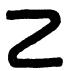
\includegraphics[keepaspectratio]{images/part002_ad0e6982551a0008e23df60b46a8b3d8f866f5ecbe9521df85283d9b8fea8d5c.jpg}}

读者应注意不要假定 \(a + m = b + m\) 对所有基数 m 都蕴含 a = b（参见 §6）；* 然而我们稍后将看到，若 m 是有限的，则这一蕴含关系成立（§5，第 2 号，命题 3，推论 4 以及 §6，第 3 号，定理 3，推论 4）。*

\subsection{基数的指数运算}

定义 4. 设 a 和 b 为基数。从 b 到 a 的映射所构成的集合的基数记为 \(\mathfrak{a}^{\mathfrak{b}}\) ，此处为记号上的滥用。

这里符号的滥用在于， \(a^{b}\) 已经表示从 b 到 a 的映射的图像集合（第二章，§5，第 3 号），而这个集合不一定是基数（习题 2）。从上下文中总能清楚地看出该符号 \(a^{b}\) 应取哪种含义.

命题 9. 设 X 和 Y 是两个集合，a 和 b 分别是它们的基数。则集合 \(X^{Y}\) 的基数为 \(a^{b}\) .

因为存在一个从 \(\mathbf{X}^{\mathrm{Y}}\) 到映射集合（从 \(\mathfrak{b}\) 到 \(\mathfrak{a}\) 中的映射所成的集合）上的双射 (第二章，§5，第2号，命题2，推论)。

命题10。设 \(\mathfrak{a}\) 与 \(\mathfrak{b}\) 是基数，且令 \(\mathbf{I}\) 是一个集合，使得 Card (I) = \(\mathfrak{b}\) 。如果 \(\mathfrak{a}_{\iota} = \mathfrak{a}\) （对于所有 \(\iota \in \mathbf{I}\) ），我们有 \(\mathfrak{a}^{\mathfrak{b}} = \underset{\iota \in \mathbf{I}}{\mathsf{P}}\mathfrak{a}_{\iota}\) .

这由一族集合的乘积作为函数图集合的定义得出（第二章，§5，第3号）。

推论1. 设 \(\mathfrak{a}\) 为一个基数，并令 \((\mathfrak{b}_t)_{t\in I}\) 为一个基数族。则

\[
\mathfrak{a}^{\sum_{i \in I} \mathfrak{b}_i} = \underset {i \in I} {\mathbf {P}} \mathfrak{a}^{\mathfrak{b}_i}.
\]

设 S 为诸集合 \(\mathfrak{b}_i\) 的和，并令 \(a_s = a\) （对于所有 \(s \in S\) ）。待证等式的两边随后都等于 \(\underset{s \in S}{\mathsf{P}} a_s\) ，这依据命题10以及乘积的结合律公式（第3号，命题5(b)）。

推论2。设 \((\mathfrak{a}_i)_{i\in I}\) 是一族基数，且设 \(\mathfrak{b}\) 是一个基数。则

\[
\left(\underset {i \in I} {\mathbf {P}} a _ {i}\right) ^ {b} = \underset {i \in I} {\mathbf {P}} a _ {i} ^ {b}.
\]

令 \(a_{i\beta} = a_i\) （对于每一对 \((i, \beta) \in I \times b\) ）。那么，根据乘积的结合性，我们有

\[
\left(\underset {i \in I} {\mathsf {P}} a _ {i}\right) ^ {\mathfrak {b}} = \underset {\beta \in \mathfrak {b}} {\mathsf {P}} \left(\underset {i \in I} {\mathsf {P}} a _ {i \beta}\right) = \underset {i \in I} {\mathsf {P}} \left(\underset {\beta \in \mathfrak {b}} {\mathsf {P}} a _ {i \beta}\right) = \underset {i \in I} {\mathsf {P}} a _ {i} ^ {\mathfrak {b}}.
\]

推论3。设 \(a, b, c\) 是基数。则 \(a^{bc} = (a^{b})^{c}\) .

令 \(\mathfrak{b}_{\gamma} = \mathfrak{b}\) （对于所有 \(\gamma \in \mathfrak{c}\) ）。则

\[
a ^ {b c} = a ^ {\sum_ {\gamma \in c} b _ {\gamma}} = \underset {\gamma \in c} {\mathbf {P}} a ^ {b _ {\gamma}} = (a ^ {b}) ^ {c}
\]

根据推论1。

命题11。设 \(\mathfrak{a}\) 是一个基数。则 \(\mathfrak{a}^0 = 1\) , \(\mathfrak{a}^1 = \mathfrak{a}\) , \(1^{\mathfrak{a}} = 1\) ；以及 \(0^{\mathfrak{a}} = 0\) （若 \(\mathfrak{a} \neq 0\) ）.

因为存在唯一的从 \(\varnothing\) 到任意给定集合中的映射（即图形为空集的映射）；由单个元素组成的集合到任意集合X的映射之集与X等势（第二章，§5，第3号）；存在唯一一个从任意集合到由单个元素组成的集合的映射；最后，不存在从非空集合到 \(\varnothing\) 的映射。

请特别注意， \(0^{0}=1\) .

命题12。设X为一个集合，并设a为其基数。则 \(\mathfrak{P}(X)\) （\(X\) 的所有子集所成的集合）的基数是 \(2^{\mathfrak{a}}\) 。

令 \(\alpha\) 与 \(\beta\) 为基数2的元素。对于X的每个子集Y，令 \(f_{\mathbf{Y}}\) 为 X 到 2 中的映射，定义为 \(f_{\mathbf{Y}}(x) = \alpha\) （若 \(x \in \mathbf{Y}\) ）且 \(f_{\mathbf{Y}}(x) = \beta\) （若 \(x \in \mathbf{X} - \mathbf{Y}\) ）. 设 \(u\) 为映射 \(\mathbf{Y} \to f_{\mathbf{Y}}\) （从 \(\mathfrak{P}(\mathbf{X})\) 到 \(2^{\mathbf{x}}\) 中的映射）。反之，对于每个将X映入2的映射 \(g\) ，我们让它对应于X的子集 \(-g^{1}(\alpha)\) ，并且令 \(v\) 为映射 \(g \to -g^{1}(\alpha)\) （从 \(2^{\mathbf{x}}\) 到 \(\mathfrak{P}(\mathbf{X})\) 中的映射）. 显然， \(u \circ v\) 与 \(v \circ u\) 分别是 \(2^{\mathbf{x}}\) 与 \(\mathfrak{P}(\mathbf{X})\) 的恒等映射；因此 \(u\) 与 \(v\) 是双射（第二章，§3，第8号，命题8，推论），因此 Card \((\mathfrak{P}(\mathbf{X})) = 2^{\mathbf{a}}\) .

\subsection{序关系与基数上的运算}

命题13. 设 \(\mathfrak{a}\) 与 \(\mathfrak{b}\) 是基数。则 \(\mathfrak{a} \geqslant \mathfrak{b}\) 当且仅当存在一个基数 \(\mathfrak{c}\) 使得 \(\mathfrak{a} = \mathfrak{b} + \mathfrak{c}\) .

因为关系 \(a \geqslant b\) 意味着存在a的一个与b等势的子集B（第2号），即a与b和某个集合c所成的和集等势。

\pandocbounded{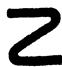
\includegraphics[keepaspectratio]{images/part002_f1d2aad8dae595af04a38c0526d2ebc1f30c28017ae785c1fe861e266dceeae2.jpg}}

如果 \(a \geqslant b\) ，通常存在许多基数 \(c\) 使得 \(a = b + c\) （参见§6）；因此，一般来说，不可能定义两个这样的基数的“差” \(a - b\) （参见§5，第2号）。

命题14。设 \((\mathfrak{a}_i)_{i\in I}\) 与 \((\mathfrak{b}_i)_{i\in I}\) 是两族基数，它们都由同一个集合 \(I\) 索引，并且使得 \(\mathfrak{a}_i\geqslant \mathfrak{b}_i\) （对于所有 \(i\in I\) ）。则

\[
\sum_ {i \in I} a _ {i} \geqslant \sum_ {i \in I} b _ {i}, \quad \mathbf {P} _ {i \in I} a _ {i} \geqslant \mathbf {P} _ {i \in I} b _ {i}.
\]

第二个不等式由集合乘积之间的包含关系得出（第二章，§5，第4号，命题6，推论3）。至于第一个不等式，如果集合E是某个族 \((\mathbf{A}_{t})_{t\in\mathbf{I}}\) 的互不相交子集的并集，且如果 \(B_{t}\subset A_{t}\) 对于所有 \(t\in I\) ，则 \(B_{t}\) 也是两两不相交的，并且 \(\bigcup_{i}B_{i}\subset\bigcup_{i}A_{i}\) （第二章，§4，第2号）。

推论1. 设 \((\mathfrak{a}_i)_{t \in I}\) 为一族基数。对于每个子集 \(J\) （ \(I\) 的子集），我们有 \(\sum_{i \in J} \mathfrak{a}_i \leqslant \sum_{i \in I} \mathfrak{a}_i\) 。如果还有 \(\mathfrak{a}_i \neq 0\) （对于所有 \(i \in I - J\) ），那么 \(\mathsf{P}_{i \in J} \mathfrak{a}_i \leqslant \mathsf{P}_{i \in I} \mathfrak{a}_i\) 。置 \(\mathfrak{b}_i = \mathfrak{a}_i\) （若 \(i \in J\) ），以及 \(\mathfrak{b}_i = 0\) （相应地， \(\mathfrak{b}_i = 1\) ）（若 \(i \in I - J\) ）。然后应用命题14，并注意到关系 \(\mathfrak{a} \neq 0\) 蕴含 \(\mathfrak{a} \geqslant 1\) .

推论2。如果 \(\mathfrak{a}\) , \(\mathfrak{a}'\) , \(\mathfrak{b}\) , \(\mathfrak{b}'\) 是基数，使得 \(\mathfrak{a} \leqslant \mathfrak{a}'\) , \(\mathfrak{b} \leqslant \mathfrak{b}'\) ，以及 \(\mathfrak{a}' > 0\) ，那么 \(\mathfrak{a}^{\mathfrak{b}} \leqslant {\mathfrak{a}'}^{\mathfrak{b}'}\) .

由命题10和命题14可得 \(a^b \leqslant a'^b\) ，由命题10和命题14的推论1可得 \(a'^b \leqslant a'^{b'}\) 。

定理2（康托尔）。对于每个基数a，我们有 \(2^{\mathfrak{a}} > \mathfrak{a}\) .

我们有 \(\operatorname{Card}(\mathfrak{P}(\mathfrak{a})) = 2^{\mathfrak{a}}\) （第5号，命题12）。映射 \(x \to \{x\} (x \in \mathfrak{a})\) 是 \(\mathfrak{a}\) 到 \(\mathfrak{P}(\mathfrak{a})\) 中的一个单射，由此 \(\mathfrak{a} \leqslant 2^{\mathfrak{a}}\) 。因此只需证明 \(\mathfrak{a} \neq 2^{\mathfrak{a}}\) ，即对于每一个映射 \(f\) （从 \(\mathfrak{a}\) 到 \(\mathfrak{P}(\mathfrak{a})\) 中的映射），图像 \(f(\mathfrak{a})\) 都不同于 \(\mathfrak{P}(\mathfrak{a})\) . 设 \(\mathbf{X}\) 是所有 \(x \in \mathfrak{a}\) （满足 \(x \notin f(x)\) ）所成的集合。如果 \(x \in \mathbf{X}\) ，我们有 \(x \notin f(x)\) ，由此 \(f(x) \neq \mathbf{X}\) ；若 \(x \in \mathfrak{a} - \mathbf{X}\) ，我们有 \(x \in f(x)\) 并且 \(x \notin \mathbf{X}\) ，由此 \(f(x) \neq \mathbf{X}\) 。这表明 \(\mathbf{X} \notin f(\mathfrak{a})\) 并证明了该定理。

推论。不存在一个集合，它以每个基数作为元素。

如果U是这样的集合，那么就会存在一个集合S，它是集合族 \((\mathbf{X})_{\mathbf{x}\in\mathbf{U}}\) 的和，使得每个基数都与S的某个子集等势。特别地，设 \(\mathfrak{S}=\operatorname{Card}(\mathbf{S})\) ；由于 \(2^{S}\) 是一个基数，我们就会有 \(2^{S}\leqslant S\) ，这与定理2矛盾。

\section{自然整数。有限集合}

\subsection{整数的定义}

定义1。一个基数 \(\mathfrak{a}\) 称为有限的，如果 \(\mathfrak{a} \neq \mathfrak{a} + 1\) 。有限基数也称为自然整数（如果没有混淆风险，简称为整数（*））。一个集合 \(\mathbf{E}\) 称为有限的，如果Card (E)是有限基数；此时Card (E)称为 \(\mathbf{E}\) 的元素个数.

一个族（第二章，§3，第4号）称为有限的，如果其指标集是有限的。

当我们说某种类型的对象的个数是整数m时，我们的意思是这些对象是一个有限集合的元素，该集合的元素个数为m。元素个数为m的集合也称为m个元素的集合。

命题1。基数a是有限的当且仅当a + 1是有限的。

因为关系 \(\mathfrak{a} = \mathfrak{b}\) 与 \(\mathfrak{a} + 1 = \mathfrak{b} + 1\) （基数 \(\mathfrak{a}\) 与 \(\mathfrak{b}\) 之间的关系）是等价的（§3，第4号，命题8）；因此关系 \(\mathfrak{a} \neq \mathfrak{a} + 1\) 与 \(\mathfrak{a} + 1 \neq (\mathfrak{a} + 1) + 1\) 是等价的。

显然 \(0 \neq 1\) ；因此0是整数。由此可知1和2是整数。基数 \(2 + 1\) 与 \((2 + 1) + 1\) 是整数，分别记为3和4。

\subsection{整数之间的不等式}

命题2. 设 \(n\) 是一个整数。那么每个基数 \(\mathfrak{a}\) （满足 \(\mathfrak{a} \leqslant n\) ）都是整数。如果 \(n \neq 0\) ，则存在唯一的整数 \(m\) 使得 \(n = m + 1\) ，且关系 \(a < n\) 等价于 \(a \leqslant m\) 。

如果 \(\mathfrak{a} \leqslant n\) ，则存在一个基数 \(\mathfrak{b}\) 使得 \(n = \mathfrak{a} + \mathfrak{b}\) （§3，第6号，命题13）。那么 \((\mathfrak{a} + 1) + \mathfrak{b} = (\mathfrak{a} + \mathfrak{b}) + 1 = n + 1\) （§3，第3号，命题5，推论）；并且由于 \(n \neq n + 1\) ，我们有

\[
(a + 1) + b \neq a + b.
\]

因此， \(\mathfrak{a} + 1 \neq \mathfrak{a}\) ，这意味着 \(\mathfrak{a}\) 是一个整数。如果 \(n \neq 0\) ，我们有 \(n \geqslant 1\) （§3，第2号），因此存在唯一的基数 \(m\) 使得 \(n = m + 1\) （§3，第6号，命题13和第4号，命题8）。由于 \(m \leqslant n\) , \(m\) 是整数，根据已经证明的结果。最后，如果一个整数 \(a\) 满足 \(a < n\) ，我们有 \(n = a + b\) ，其中 \(b \neq 0\) (§3，第6号，命题13)；因为 \(b\) 是一个整数，我们有 \(b = c + 1\) 并且 \(n = m + 1 = (a + c) + 1\) . 由此可知 \(m = a + c\) （§3，第4号，命题8），因此 \(a \leqslant m\) 。反之，若 \(a \leqslant m\) ，我们有

\[
a \leqslant m + 1 = n;
\]

并且如果 \(a = n = m + 1\) ，我们就会有 \(a > m\) ，与假设相反。

推论1. 有限集的每个子集都是有限的。

推论2. 若X是有限集E的子集且X ≠ E，则

\[
\text { Card } (\mathbf {X}) <   \text { Card } (\mathbf {E}).
\]

因为 X 包含于 \(X'\) ——E 的由单个元素组成的子集的补集——中；我们有 \(\text{Card}(X) \leqslant \text{Card}(X')\) 并且 \(\text{Card}(E) = \text{Card}(X') + 1\) ，因此（命题2） \(\text{Card}(X') < \text{Card}(E)\) 且更有 \(\text{Card}(X) < \text{Card}(E)\) .

定义1表明，反之，若E是一个集合使得

\[
\operatorname{Card} (\mathbf {X}) <   \operatorname{Card} (\mathbf {E})
\]

对于E的每一个满足 \(X \neq E\) 的子集X，则E是有限的。

推论3。如果 \(f\) 是从有限集合 \(\mathbf{E}\) 到一个集合 \(\mathbf{F}\) 的映射，那么 \(f(\mathbf{E})\) 是 \(\mathbf{F}\) 的一个有限子集。

因为 Card \((f(\mathbf{E}))\leqslant\) Card (E)（§ 3，第 2 号，命题 3）。

推论4. 设E和F是两个具有相同元素个数的有限集合，并设f是从E到F的一个映射。则以下陈述是等价的：

\begin{enumerate}
\def\labelenumi{(\alph{enumi})}
\item
  \(f\) 是一个单射；
\item
  \(f\) 是一个满射；
\item
  \(f\) 是双射。
\end{enumerate}

只需证明(a)与(b)等价即可。若 \(f\) 是单射，则 \(\operatorname{Card}(f(\mathbf{E})) = \operatorname{Card}(\mathbf{E}) = \operatorname{Card}(\mathbf{F})\) ，由此 \(f(\mathbf{E}) = \mathbf{F}\) （推论2）。如果 \(f\) 不是单射，设 \(x\) 与 \(x'\) 为 \(\mathbf{E}\) 中满足 \(x \neq x'\) 且 \(f(x) = f(x')\) 的两个元素。那么，令 \(\mathbf{E}' = \mathbf{E} - \{x\}\) ，我们有 \(f(\mathbf{E}') = f(\mathbf{E})\) ，由此 \(\operatorname{Card}(f(\mathbf{E})) \leqslant \operatorname{Card}(\mathbf{E}') < \operatorname{Card}(\mathbf{E})\) 根据推论2；但由于 \(\operatorname{Card}(\mathbf{F}) = \operatorname{Card}(\mathbf{E})\) ，由此可得 \(f(\mathbf{E}) \neq \mathbf{F}\) .

\subsection{归纳原理}

C61（归纳原理）。设 \(\mathbb{R}\{n\}\) 是理论 \(\mathfrak{C}\) 中的一个关系（其中 \(n\) 不是 \(\mathfrak{C}\) 的常数）。假设关系

\[
\mathrm{R} \{0 \} \text { 且 } (\forall n) ((n \text { 是整数   且 } \mathrm{R} \{n \}) \Longrightarrow \mathrm{R} \{n + 1 \})
\]

在 \(\mathfrak{C}\) 中是定理。在这些条件下，关系

\[
(\forall n) ((n \text {   是整数   }) \Longrightarrow R \{n \})
\]

在 \(\mathfrak{C}\) 中是定理.

我们将用反证法论证。假设关系

\[
(\exists n) (n \text {   是整数   且   } (\text { 非   } R \{n \}))
\]

成立。设 \(q\) 是一个整数，使得“非 \(\mathbb{R}\{q\}\) ”（辅助常数法；参见第一章§3第3号及§4第1号）。整数 \(n\) （满足“ \(n \leqslant q\) 以及（非 \(\mathbb{R}\{n\}\) )''的）构成一个良序非空集合（§3，第2号，注记），因此它有一个最小元素 \(s\) 。如果 \(s = 0\) ，则“非 \(\mathbb{R}\{0\}\) ''，与假设矛盾。若 \(s > 0\) ，那么 \(s = s' + 1\) ，其中 \(s'\) 是一个满足 \(s' < s\) 的整数（第2号，命题2）。根据 \(s\) 的定义，我们有 \(\mathbb{R}\{s'\}\) ，但随后假设蕴含 \(\mathbb{R}\{s\}\) 是真的，这与 \(s\) 的定义相矛盾.

为了应用归纳原理，特别需要证明关系

\[
(n \text {   是整数   且   } R \{n \}) \Longrightarrow R \{n + 1 \}.
\]

为此目的，通常使用辅助假设的方法（第一章，§3，第3号），正是因为这个原因，关系“n是整数且R\{n\}''（甚至R\{n\}）被称为归纳假设。

注记。有许多不同的准则经常以“归纳原理”之名被使用。它们都可以很容易地从C61推导出来，我们在此指出其中最重要的几个：

\begin{enumerate}
\def\labelenumi{(\arabic{enumi})}
\tightlist
\item
  让 \(\mathbf{S}\{n\}\) 为关系
\end{enumerate}

\((\forall p)((n \text{ 是整数 且 } p \text{ 是整数 且 } p < n) \Longrightarrow \mathbb{R}\{p\})\)

并且假设 \(S\{n\}\) 蕴含 \(R\{n\}\) 。则关系

\[
(\forall n) ((n \text {   是整数   }) \Longrightarrow R \{n \})
\]

是真的。因为关系 \(S\{0\}\) 是真的，并且根据假设 \(S\{n\}\) 蕴含 \(R\{n\}\) ；由于关系 \(m < n + 1\) 等价于 \(m \leqslant n\) （第2号，命题2），关系 \(S\{n + 1\}\) 等价于“ \(S\{n\}\) 并且 \(R\{n\}\) ''，因此， \(S\{n\}\) 蕴含 \(S\{n + 1\}\) 。因此，准则C61证明了关系

\[
(\forall n) ((n \text {   是整数   }) \Longrightarrow \mathrm{S} \{n \})
\]

是真的，并且由于 \(\mathbf{S}\{n\}\) 蕴含 \(\mathbf{R}\{n\}\) ，关系

\[
(\forall n) ((n \text {   是整数   }) \Longrightarrow R \{n \})
\]

为真。

\begin{enumerate}
\def\labelenumi{(\arabic{enumi})}
\setcounter{enumi}{1}
\tightlist
\item
  设 \(k\) 为一个整数，设 \(\mathbf{R}\{n\}\) 是一个关系，使得关系
\end{enumerate}

\[
\mathrm{R} \{k \} \text { 且 } (\forall n) ((n \text { 是整数 } \geqslant k \text { 且 } \mathrm{R} \{n \}) \Longrightarrow \mathrm{R} \{n + 1 \})
\]

成立。那么关系

\[
(\forall n) ((n \text {   是整数   } \geqslant k) \Longrightarrow \mathrm{R} \{n \})
\]

成立（“从 \(k\) 开始的归纳”）。令 \(S\{n\}\) 为关系

\[
(n \geqslant k) \Longrightarrow \mathrm{R} \{n \}.
\]

然后通过分情况讨论的方法，我们看到S\{0\} 成立。另一方面，容易验证关系

\[
(n \text {   是整数   且   } S \{n \}) \Longrightarrow S \{n + 1 \}
\]

成立。由C61可知关系

\[
(n \text {   是整数) } \implies \mathrm{S} \{n \}
\]

成立，这证明了我们的断言。

\begin{enumerate}
\def\labelenumi{(\arabic{enumi})}
\setcounter{enumi}{2}
\tightlist
\item
  让 \(a\) 与 \(b\) 是两个整数，使得 \(a \leqslant b\) ，并且让 \(R\{n\}\) 是一个满足
\end{enumerate}

\[
\mathrm{R} \left\{a \right\} \text {   且   } (\forall n) ((n \text {   是整数   且   } a \leqslant n <   b \text {   且   } \mathrm{R} \left\{n \right\}) \Longrightarrow \mathrm{R} \left\{n + 1 \right\}).
\]

那么关系

\[
(\forall n) ((n \text {   是整数   且   } a \leqslant n \leqslant b) \Longrightarrow \mathrm{R} \{n \})
\]

成立。证明与前一情形类似；我们取 S\{n\} 为关系“(a ≤ n \textless{} b) ⇒ R\{n\}''（“限制在区间上的归纳”）。

\begin{enumerate}
\def\labelenumi{(\arabic{enumi})}
\setcounter{enumi}{3}
\tightlist
\item
  让 \(a, b\) 是两个整数，使得 \(a \leqslant b\) ，并且让 \(\mathbf{R}\{n\}\) 是一个满足
\end{enumerate}

\(R\{b\}\) 并且 \((\forall n)((n \text{ 是整数 且 } a \leqslant n < b \text{ 且 } R\{n + 1\}) \Longrightarrow R\{n\}).\)

那么关系

\[
(\forall n) ((n \text {   是整数   且   } a \leqslant n \leqslant b) \Longrightarrow \mathrm{R} \{n \})
\]

是真的。因为我们有关系

（n 是一个整数且 \(a \leqslant n < b\) 以及（非 \(\mathbf{R}\{n\}\) ) \(\Longrightarrow\) 不 \(\mathbf{R}\{n + 1\}\) .

如果对于某个 \(n\) 使得 \(a \leqslant n \leqslant b\) 我们有（并非 \(\mathbf{R}\{n\}\) ），则由(3)可推出（并非 \(\mathbf{R}\{b\}\) ），这与假设矛盾，因此结论成立（“反向归纳”）。

\subsection{有序集合的有限子集}

命题3. 设E是一个右定向预序集（相应地，一个格，相应地，一个全序集）。则E的每个非空有限子集都有上界（相应地，有最小上界和最大下界，相应地，有最大元素和最小元素）。

证明通过对所考虑子集的元素个数n进行归纳。当n = 1时，结论是平凡的。设X是 E 的由 \(n + 1\) 个元素组成的子集（其中 \(n \geqslant 1\) ），并令 \(X = Y \cup \{x\}\) ，其中Y有n个元素，因此非空。归纳假设蕴含存在 Y 的一个上界（相应地，最小上界，相应地，最大元素）y。由于E是右有向的（相应地，一个格，相应地，全序的）， \(\{x, y\}\) 有一个上界（相应地，最小上界，相应地，最大元素），它显然是X的一个上界（相应地，最小上界，相应地，最大元素）。

推论1. 每个全序有限集都是良序的，并且有一个最大元素。

推论2. 每个有限有序集都有一个极大元素。

因为这样的集合由推论1（参见§2，第4号，定理2）是归纳的。

\subsection{有限特征的性质}

定义2. 设E是一个集合。E的子集的一个集合S称为具有有限特征，如果关系X∈S等价于关系“X的每个有限子集都属于S”。

一个性质 \(P\{X\}\) 关于集合E的子集X，如果使 \(P\{X\}\) 成立的E的子集X的集合具有有限特征，则称该性质具有有限特征。

\minorheading{示例}

\begin{enumerate}
\def\labelenumi{(\arabic{enumi})}
\tightlist
\item
  一个有序集合E的全序子集的集合具有有限特征。事实上，E的一个子集X是全序的当且仅当X的每个由两个元素组成的子集都是全序的。
\end{enumerate}

*（2）一个模的所有自由子集的集合具有有限特征。一个域的扩张的所有代数自由子集的集合也是如此。

\begin{enumerate}
\def\labelenumi{(\arabic{enumi})}
\setcounter{enumi}{2}
\tightlist
\item
  一个模E的子模的集合不具有有限特征，因为E的一个子模的有限子集不一定是E的子模。*
\end{enumerate}

定理1. 集合E的子集的一个具有有限特征的集合S（按包含关系排序时）有一个极大元素。

由§2第4号的定理2，只需证明 \(\mathfrak{S}\) 是归纳的。为此我们将证明：如果 \(\mathfrak{G}\) 是 \(\mathfrak{S}\) 的任意一个按包含关系全序的子集，则 \(\mathfrak{G}\) 的诸集合的并集X属于 \(\mathfrak{S}\) (§2，第4号，定理2，推论2)。由于 \(\mathfrak{S}\) 具有有限特征，只需证明X的每个有限子集Y都属于 \(\mathfrak{S}\) 。现在，对于每个 \(y \in Y\) ，存在一个集合 \(Z_y \in \mathfrak{G}\) 使得 \(y \in Z_y\) 。由于集合族 \(Z_y\) ( \(y \in Y\) )是有限的且按包含关系全序排列，它有一个最大元素S（第4号，命题3的推论1）；换言之，存在一个集合 \(S \in \mathfrak{G}\) 使得 \(Y \subset S\) 。但由于 \(S \in \mathfrak{S}\) ，且由于Y是S的有限子集，我们有 \(Y \in \mathfrak{S}\) 因为 \(\mathfrak{S}\) 具有有限特征；这就完成了证明。

\section{整数的性质}

\subsection{整数与有限集上的运算}

命题1. 设 \((a_i)_{i\in I}\) 是一个整数的有限族。则基数 \(\sum_{i\in I}a_i\) 与 \(\prod_{i\in I}a_i\) 是整数。

让我们首先证明，如果 \(a\) 与 \(b\) 是整数，则 \(a + b\) 也是整数。我们对 \(b\) 进行归纳。该命题在 \(b = 0\) 时成立，因为 \(a + 0 = a\) 。如果 \(a + b\) 是整数，则 \((a + b) + 1\) 也是整数 ( \(\S 4\) ，第1号，命题1）。但 \((a + b) + 1 = a + (b + 1)\) ( \(\S 3\) ，第3号，命题5的推论）；因此 \(a + (b + 1)\) 是整数，从而 \(a + b\) 对所有整数 \(b\) 而言都是整数.

接下来对 \(n = \operatorname{Card}(\mathbf{I})\) 作归纳，证明 \(\sum_{i \in \mathbf{I}} a_i\) 是整数。当 \(n = 0\) 时这是显然的，因为 \(\mathbf{I} = \emptyset\) 且 \(\sum_{i \in \mathbf{I}} a_i = 0\) 。如果 \(\operatorname{Card}(\mathbf{I}) = n + 1\) ，可写成 \(\mathbf{I} = \mathbf{J} \cup \{k\}\) ，其中 \(\operatorname{Card}(\mathbf{J}) = n\) 且 \(k \notin \mathbf{J}\) 。于是

\[
\sum_ {i \in \mathbf {I}} a _ {i} = a _ {k} + \sum_ {i \in \mathbf {J}} a _ {i}
\]

（§ 3，第 3 号，命题 5）。归纳假设是 \(\sum_{i\in J}a_i\) 是整数；因此 \(a_{k} + \sum_{i\in J}a_{i}\) 也是整数，这由证明的第一段得出。这表明 \(\sum_{i\in I}a_{i}\) 对所有 \(n\) 都是整数.

由于两个整数a和b的乘积ab是有限个全等于a的整数之和（§3，第4号，命题6，推论2），因此ab是整数。我们将通过对n = Card (I)进行归纳来证明 \(\prod_{i\in I}a_{i}\) 是一个整数。这对n = 0成立，因为此时

\[
\prod_ {i \in \mathbf {I}} a _ {i} = 1.
\]

若 Card (I) = n + 1，则（沿用上述记号）我们有

\[
\prod_ {i \in \mathbf {I}} a _ {i} = a _ {k}. \prod_ {i \in \mathbf {J}} a _ {i}
\]

（§3，第3号，命题5），因此归纳假设蕴含 \(\prod_{i\in I}a_i\) 是一个整数。因此 \(\prod_{i\in I}a_i\) 对所有 \(n\) 都是整数.

推论1. 有限集合的有限族 \((\mathbf{X}_i)_{i\in \mathbf{I}}\) 的并集E是有限集合。

因为族 \((\mathbf{X}_{i})\) 的和 S 是有限的；并且由于存在从 S 到 E 的满射（第二章，§4，第 8 号），集合 E 是有限的（§4，第 2 号，命题 2，推论 3）。

推论 2. 有限个有限集合的乘积是有限集合。

推论3。如果 \(a\) 与 \(b\) 是整数，则 \(a^b\) 是一个整数。

因为 \(a^b\) 是一个有限整数族的乘积，该族中每个整数都等于 \(a\) （§3，第5号，命题10）。

推论4. 有限集合E的子集所构成的集合是有限的。

因为其基数为 \(2^{\text{Card (E)}}\) ( \(\S 3\) ，第5号，命题12）。

\subsection{整数之间的严格不等式}

命题2. 设 \(a\) 与 \(b\) 是两个整数。则 \(a < b\) 当且仅当存在一个整数 \(c > 0\) 使得 \(b = a + c\) .

如果 \(a < b\) ，则存在一个基数 \(c \leqslant b\) （使得 \(c\) 是一个整数（ \(\S 4\) ，第2号，命题2））使得 \(b = a + c\) ( \(\S 3\) ，第6号，命题13）；若 \(a \neq b\) ，我们必须有 \(c \neq 0\) 。反之，若 \(b = a + c\) 并且 \(c \neq 0\) ，那么 \(c \geqslant 1\) ，因此 \(a < a + 1 \leqslant a + c = b\) .

命题3。设 \((a_i)_{i \in I}\) 与 \((b)_{i \in I}\) 是两个整数有限族，使得 \(a_i \leqslant b_i\) 对于每一个 \(i \in I\) 并且 \(a_i < b_i\) 对于至少一个指标 \(i\) 。然后

\[
\sum_ {i \in \mathbf {I}} a _ {i} <   \sum_ {i \in \mathbf {I}} b _ {i}.
\]

如果还有 \(b_{i} > 0\) 对于每一个 \(i \in \mathbf{I}\) ，那么

\[
\prod_ {i \in I} a _ {i} <   \prod_ {i \in I} b _ {i}.
\]

让 \(j\) 是一个指标使得 \(a_{j} < b_{j}\) ，并且让 \(J = I - \{j\}\) 。然后

\[
b _ {j} = a _ {j} + c _ {j}
\]

其中 \(c_{j} > 0\) （命题2），因此（§3，第6号，命题14）

\[
\sum_ {i \in \mathbf {I}} b _ {i} = a _ {j} + c _ {j} + \sum_ {i \in \mathbf {J}} b _ {i} \geqslant c _ {j} + a _ {j} + \sum_ {i \in \mathbf {J}} a _ {i} = c _ {j} + \sum_ {i \in \mathbf {I}} a _ {i}.
\]

由于 \(c_{j} > 0\) ，命题的第一部分由命题2得出。同样地

\[
\prod_ {i \in I} b _ {i} = (a _ {j} + c _ {j}) \prod_ {i \in J} b _ {i} = a _ {j}. \prod_ {i \in J} b _ {i} + c _ {j}. \prod_ {i \in J} b _ {i} \geqslant \prod_ {i \in I} a _ {i} + c _ {j}. \prod_ {i \in J} b _ {i}.
\]

由于 \(c_{j}\) 以及所有 \(b_{i}\) 是 \(\neq 0\) ，乘积 \(c_{j}\) . \(\prod_{i \in \mathbb{J}} b_{i}\) 是 \(\neq 0\) （§3，第4号，命题7）；因此命题的第二部分成立。

推论1. 设 \(a, a',\) 与 \(b\) 是整数，使得 \(a < a'\) 且 \(b > 0\) 。则 \(a^b < a'^b\) .

我们只需将 \(a^b\) 与 \(a'^b\) 表示为整数的有限族之积（§3，第5号，命题10）并应用命题3，注意到关系 \(a < a'\) 蕴含 \(a' > 0\) .

推论2。设 \(a, b\) 与 \(b'\) 是整数，使得 \(a > 1\) 且 \(b < b'\) ；则 \(a^b < a^{b'}\) .

因为存在一个整数 \(c > 0\) 使得 \(b' = b + c\) （命题2）；由于 \(c \geqslant 1\) ，我们有 \(a^c \geqslant a > 1\) ，由此 \(a^{b'} = a^b a^c > a^b\) .

推论3。设 \(a, b, b'\) 是整数（相应地，满足 \(a > 0\) 的整数）。则 \(a + b = a + b'\) （相应地， \(ab = ab'\) ）当且仅当 \(b = b'\) .

推论4. 若 \(a\) 与 \(b\) 是满足 \(a \leqslant b\) 的整数，则存在唯一的整数 \(c\) 使得 \(b = a + c\) .

\(c\) 的存在性由第3节第6号中的命题13得出，其唯一性则由上面的推论3得出。

整数 \(c\) （满足 \(b = a + c\) ，其中 \(a \leqslant b\) ）称为整数 \(b\) 与 \(a\) 的差，并记作 \(b - a\) 。容易验证，如果 \(a, b, a', b'\) 是满足 \(a \leqslant b\) 并且 \(a' \leqslant b'\) 的整数，那么

\[
(b - a) + (b ^ {\prime} - a ^ {\prime}) = (b + b ^ {\prime}) - (a + a ^ {\prime}).
\]

\subsection{整数集合中的区间}

每个整数集合，作为基数集合，都是良序的（§ 3，第 2 号，定理 1）。此外，对于每个整数 \(a\) ，关系“ \(x\) 是一个基数，且 \(x \leqslant a\) '' 在 \(x\) （第3节，第2号，定理1后的注记）中是收集性的，并且满足此关系的 \(x\) 的集合是一个整数集合（第4节，第2号，命题2），因此可以记为 {[}0, a{]}.

命题4。设 \(a\) 与 \(b\) 是整数。则映射 \(x \to a + x\) 是区间 \([0, b]\) 到区间 \([a, a + b]\) 上的严格递增同构，而 \(y \to y - a\) 是逆同构。

显然，关系 \(0 \leqslant x \leqslant b\) 蕴含 \(a \leqslant a + x \leqslant a + b\) . 由第2号命题3，映射 \(x \to a + x\) 严格递增（因而是单射）。最后，关系 \(a \leqslant y \leqslant a + b\) 蕴含 \(y = a + x\) ，其中 \(x \geqslant 0\) 且 \(a + x \leqslant a + b\) ，由此 \(x \leqslant b\) （第2号，命题3）。证明完成。

命题5. 如果 \(a\) 与 \(b\) 是满足 \(a \leqslant b\) 的整数，则区间 \([a, b]\) 是一个有限集合，其元素个数为 \(b - a + 1\) .

根据命题4，我们可以将自身限制在以下情形： \(a=0\) 。证明通过对 \(b\) 进行归纳。如果 \(b=0\) ，结果是显然的。关系 \(0 \leqslant x \leqslant b+1\) 等价于“ \(0 \leqslant x < b+1\) 或 \(x=b+1\) ''，且关系 \(0 \leqslant x < b+1\) 等价于 \(0 \leqslant x \leqslant b\) (§ 4，第 2 号，命题 2)；换言之，区间 \([0, b+1]\) 是 \([0, b]\) 与 \(\{b+1\}\) 的并集，且这两个集合不相交。根据归纳假设， \([0, b+1]\) 的元素个数等于 \((b+1)+1\) ，命题得证。

命题6. 对于每个有限集合 \(\mathbf{E}\) （它是全序的且具有 \(n\) 个元素 \((n \geqslant 1)\) ），存在唯一的从 \(\mathbf{E}\) 到区间 \([1, n]\) 上的同构.

由于 E 和 \([1, n]\) 都是良序的（§4，第 4 号，命题 3，推论 1）且具有相同数量的元素（命题 5），结论由 §2，第 5 号的定理 3 以及 §4，第 2 号的命题 2 的推论 2 得出。

\subsection{有限序列}

有限序列（相应地，集合 E 的元素的有限序列）是一个族（相应地，E 的元素的族），其指标集 I 是整数的有限集。I 的元素个数称为序列的长度。

设 \((t_i)_{i \in I}\) 为长度为 \(n\) 的有限序列。由第 3 号的命题 6，存在唯一的同构 \(f\) ，从区间 \([1, n]\) 到整数集合 \(I\) 上。对于每一个 \(k \in [1, n]\) , \(t_{f(k)}\) 被称为序列的第 \(k\) 项； \(t_{f(1)}\) （相应地， \(t_{f(n)}\) ）是序列的第一项（相应地，最后一项）。

设 \(P\{i\}\) 是这样一个关系：使得元素 \(i\) （满足 \(P\{i\}\) 为真）组成一个有限的整数集合。因此一个有限序列 \((t_i)_{i \in I}\) 常常写作 \((t_i)_{P\{i\}}\) 。例如，当 \(I = [a, b]\) 时，记号 \((t_i)_{a \leqslant i \leqslant b}\) 经常被使用。在相同条件下，为表示一族集合 \((X_i)_{i \in I}\) 的乘积，使用记号

\[
\prod_ {\mathrm{P} \{i \}} \mathrm{X} _ {i} \quad \text { 且 } \quad \prod_ {i = a} ^ {b} \mathrm{X} _ {i}
\]

这些记号被使用；对于并、交、基数积、基数和、* 代数中的合成法则 * 等，也有类似的记号。

\subsection{集合的特征函数}

设 E 为非空集合，A 为 E 的子集。子集 A 在 E 中的特征函数是映射 \(\varphi_{A}\) （从 E 到集合 \(\{0, 1\}\) 中的映射），定义为

\[
\varphi_ {\mathbf {A}} (x) = 1 \quad \text { 若 } \quad x \in \mathbf {A}; \qquad \varphi_ {\mathbf {A}} (x) = 0 \quad \text { 若 } \quad x \in \mathbf {E} - \mathbf {A}.
\]

显然有关系 \(\varphi_{\mathbf{A}} = \varphi_{\mathbf{B}}\) 等价于 \(\mathbf{A} = \mathbf{B}\) 。我们有 \(\varphi_{\mathbf{E}}(x) = 1\) 对于所有 \(x \in \mathbf{E}\) 并且 \(\varphi_{\emptyset}(x) = 0\) 对于所有 \(x \in \mathbf{E}\) ；这些是 \(\mathbf{E}\) 上仅有的常值特征函数。以下命题是定义的直接推论：

命题 7. 对非空集合 E 的每一对子集 A、B，我们有

\begin{enumerate}
\def\labelenumi{(\arabic{enumi})}
\tightlist
\item
\end{enumerate}

\[
\varphi_ {\mathbf {E} - \mathbf {A}} (x) = 1 - \varphi_ {\mathbf {A}} (x),\tag{2}
\]

\[
\varphi_ {\mathbf {A} \cap \mathbf {B}} (x) = \varphi_ {\mathbf {A}} (x) \varphi_ {\mathbf {B}} (x),\tag{3}
\]

\[
\varphi_ {\mathbf {A} \cup \mathbf {B}} (x) + \varphi_ {\mathbf {A} \cap \mathbf {B}} (x) = \varphi_ {\mathbf {A}} (x) + \varphi_ {\mathbf {B}} (x)
\]

对于所有 \(x \in E\) .

\subsection{欧几里得除法}

定理1. 设 \(a\) 与 \(b\) 是整数，使得 \(b > 0\) 。那么存在整数 \(q\) 与 \(r\) ，使得 \(a = bq + r\) 且 \(r < b\) ，且整数 \(q\) 与 \(r\) 由这些条件唯一确定。

关于 \(q\) 和 \(r\) 的条件等价于 \(bq \leqslant a < b(q + 1)\) 且 \(r = a - bq\) （第2号，命题2）。因此必须找到 \(q\) 使得 \(bq \leqslant a < b(q + 1)\) ；换言之， \(q\) 必须是使 \(a < b(q + 1)\) 成立的最小整数，这表明 \(q\) 和 \(r = a - bq\) 都唯一确定。为证明它们存在，注意到存在整数 \(p\) 使 \(a < bp\) ，例如 \(a + 1\) （因为 \(b > 0\) ）。设 \(m\) 为这些整数中最小的一个。由于 \(m \neq 0\) ，可写成 \(m = q + 1\) ，其中 \(q \leqslant m\) ( \(\S 4\) ，第2号，命题2）；于是 \(bq \leqslant a < b(q + 1)\) .

定义1. 采用定理1的记号，r称为a除以b的余数。如果r=0，我们说a是b的倍数，或a能被b整除，或b是a的除数，或b整除a，或b是a的因子。数q称为a除以b的商，记为 \(\frac{a}{b}\) 或a/b。

如果 \(a\) 不是 \(b\) 的倍数，数 \(q\) 称为 \(a\) 除以 \(b\) 的商的整数部分（参见一般拓扑学，第四章，第8节，第2号）。

在本章中，写作 \(a / b\) 或 \(\frac{a}{b}\) 将蕴含 \(b\) 整除 \(a\) .

关系 \(a = bq\) 并且 \(q = a / b\) 是等价的（如果 \(b > 0\) ）。每一个倍数 \(a'\) （它是倍数 \(a\) ——\(b\) 的一个倍数——的倍数）都是 \(b\) 的倍数，以及

\[
a ^ {\prime} / b = (a ^ {\prime} / a) (a / b) \quad \text { 若 } \quad a \neq 0.
\]

此外，如果 \(c\) 与 \(d\) 是 \(b\) 的倍数，那么 \(c + d\) 与 \(c - d\) （如果 \(d \leqslant c\) ）是 \(b\) 的倍数，并且我们有

\[
\frac {c + d}{b} = \frac {c}{b} + \frac {d}{b}, \quad \frac {c - d}{b} = \frac {c}{b} - \frac {d}{b}.
\]

是2的倍数的整数称为偶数，其余的称为奇数。根据定理1，奇数的形式为 \(2n + 1\) .

\subsection{展开到基b}

命题8. 设 \(b\) 是一个整数 \(> 1\) 。对于每个整数 \(k > 0\) ，令 \(\mathbf{E}_k\) 为族 \((\mathrm{J}_h)_{0 \leqslant h \leqslant k-1}\) （§2，第6号）的字典序乘积，其中所有区间都与 {[}0, \(b - 1\) {]} 相同。对于每一个 \(r = (r_0, r_1, \ldots, r_{k-1}) \in \mathbf{E}_k\) ，令 \(f_k(r) = \sum_{h=0}^{k-1} r_h b^{k-h-1}\) ；则映射 \(f_k\) 是序集 \(\mathbf{E}_k\) 到区间 {[}0, \(b^k - 1\) {]} 上的一个严格递增同构.

证明通过对 \(k\) 进行归纳。对于 \(k = 1\) ，这是定义的直接推论。对于每个 \(r = (r_0, \ldots, r_{k-1}, r_k) \in \mathbf{E}_{k+1}\) ，令

\[
\varphi (r) = \left(r _ {0}, \dots , r _ {k - 1}\right) \in \mathrm{E} _ {k}.
\]

那么映射 \(r \to (\varphi(r), r_k)\) 是 \(\mathbf{E}_{k+1}\) 到 \(\mathbf{E}_k\) 与 \(J = [0, b - 1]\) 的字典序乘积上的一个同构；这由定义直接得出。我们可以写

\[
f _ {k + 1} (r) = b \cdot f _ {k} (\varphi (r)) + r _ {k};
\]

让我们证明关系 \(r < r'\) 在 \(\mathbf{E}_{k+1}\) 中蕴含 \(f_{k+1}(r) < f_{k+1}(r')\) 。事实上，我们或者有 \(\varphi(r) < \varphi(r')\) ，或者 \(\varphi(r) = \varphi(r')\) 并且 \(r_k < r'_k\) . 在第一种情形下，归纳假设蕴含 \(f_k(\varphi(r)) < f_k(\varphi(r'))\) ，因此（§4，第2号，命题2） \(f_k(q(r')) \geqslant f_k(\varphi(r)) + 1\) ；因此

\[
f _ {k - 1} (r ^ {\prime}) \geqslant b. f _ {k} (\varphi (r)) + b > f _ {k + 1} (r),
\]

因为 \(r_k \leqslant b - 1\) （第2号，命题3）。另一方面，如果 \(\varphi(r) = \varphi(r')\) 并且 \(r_k < r_k'\) ，显然 \(f_{k+1}(r) < f_{k+1}(r')\) 。现在归纳假设表明 \(f_k(\varphi(r)) \leqslant b^k - 1\) ，由此

\[
f _ {k + 1} (r) \leqslant b (b ^ {k} - 1) + b - 1 = b ^ {k + 1} - 1.
\]

由此得出 \(f_{k+1}\) 是 \(\mathbf{E}_{k+1}\) 到区间 \([0, b^{k+1} - 1]\) 的一个子集上的一个同构；但这个区间和 \(\mathbf{E}_{k+1}\) 具有相同数量的元素，即 \(b^{k+1}\) （第3号，命题5）；因此 \(f_{k+1}\) 是一个双射（§4，第2号，命题2，推论4），证明完成。

¶ 我们现在注意到，对于每个整数 \(a\) ，我们有 \(a < b^a\) 。这是通过对 \(a\) 进行归纳来证明的；对于 \(a = 0\) ，结果是显然的，而假设 \(a < b^a\) 蕴含 \(a + 1 \leqslant b^a < b \cdot b^a = b^{a+1}\) （第2号，命题3以及第4节，第2号，命题2）。因此存在一个最小整数 \(k\) 使得 \(a < b^k\) ，然后命题8表明存在唯一的有限序列 \((r_h)_{0 \leqslant h \leqslant k-1}\) ，使得 \(0 \leqslant r_h \leqslant b - 1\) （对于 \(0 \leqslant h \leqslant k - 1\) ），并且

\[
a = \sum_ {h = 0} ^ {k - 1} r _ {h} b ^ {k - h - 1}.
\]

此外，我们必须有 \(r_{0} > 0\) ，否则根据命题8， \(a < b^{k-1}\) 。表达式

\[
\sum_ {h = 0} ^ {k - 1} r _ {h} b ^ {k - h - 1}
\]

称为整数 a 的 b 进制展开。

* 在数学中所有不涉及数值计算的部分，命题 8 主要在应用于素数 \(b\) 时是有用的. *

当整数b足够小，以至于这样做切实可行时，我们可以用一个称为数字的独特符号来表示每个整数 \textless b 。表示0和1的数字通常是0和1。设a为一个整数。 \(_{k-1}\)

并令 \(\sum_{h=0}^{r_h b^{k-h-1}}\) 为其按基 \(b\) 的展开。如果整数 \(k\) （它

在此展开中出现）足够小以至于这样做可行，通常会将整数 \(a\) 与如下的符号序列相关联：把 \(r_0r_1 \ldots r_{k-2}r_{k-1}\) 从左到右书写，然后将每个整数 \(r_i\) 替换为代表它的数字；如此得到的符号称为与 \(a\) 相关联的数值符号。然后人们常常在包含它的项和关系中用其数值符号替换 \(a\) 。

例如，若C、Q、F、D是数字，则数值符号CQ、CQF、CQFD分别与 \(Cb + Q\) , \(Cb^{2} + Qb + F\) , \(Cb^{2} + Qb^{2} + Fb + D\) 相关联。

由命题8可知，与整数a相关联的数值符号是唯一的，并且如果 \(a < b^{k}\) ，它最多包含k位数字。请注意，与整数 \(b^{k}\) 相关联的数值符号由数字1后跟k个数字0组成。

这种用数字符号表示整数的方法称为以 b 为基数的记数系统。在实际数值计算中，使用以下系统：(a) 以 2 为基数的系统，即二进制系统，其中数字为 0 和 1；(b) 十进制系统，其中数字为 0、1、2、3、4、 \(5 = 4 + 1\) , \(6 = 5 + 1\) , \(7 = 6 + 1\) , \(8 = 7 + 1\) , \(9 = 8 + 1\) ，其中 \(b\) 是整数 \(9 + 1\) （其在此系统中的数字符号因此为 10）。

自中世纪以来，十进制系统在数值计算中一直被传统地使用，在本系列中，每当我们需要明确写出一个整数时，我们都将使用它。关于求两个由数字符号给出的整数的和、差、积及商的整数部分所对应的数字符号的方法，我们请读者参阅本系列中专门讨论数值计算的部分。

\subsection{组合分析}

命题 9. 设 E 和 F 为两个集合，a 和 b 为它们的基数，f 为 E 到 F 上的一个满射，使得集合 \(\overline{f}^{1}(y)\) （其中 \(y \in F\) ）都具有相同的基数 c。则 a = bc。

因为族 \((\bar{f}^1 (y))_{\gamma \in \mathbb{F}}\) 是 \(\mathbf{E}\) 的一个划分，且划分的每个元素都是一个基数为 \(\mathfrak{c}\) 的集合；因此结果由（§ 3，第 4 号，命题 6，推论 2）得出。

定义 2. 设 \(n\) 为一个整数。乘积 \(\prod_{i < n} (i + 1)\) 记作 \(n!\) （读作“阶乘 \(n\) '').

我们有 \(0! = 1\) （第二章，§5，第 3 号）以及 \(1! = 1\) 。对于每个整数 \(n\) 我们拥有 \((n + 1)! = n!(n + 1)\) 。此关系式连同关系式 \(0! = 1\) 刻画了项 \(n!\) ，这很容易通过对 \(n\) 进行归纳而看出.

命题10。设 \(m\) 和 \(n\) 是满足 \(m \leqslant n\) 的整数。则 \(n! / (n - m)!\) 是从具有 \(m\) 个元素的集合 \(A\) 到具有 \(n\) 个元素的集合 \(B\) 的单射数目。

证明通过对 A 的元素个数 \(m \leqslant n\) 进行归纳。如果 \(m = 0\) ，结果是显然的。假设 \(m + 1 \leqslant n\) 。设 A 是一个具有 \(m + 1\) 个元素的集合，设 \(A'\) 是 A 的一个具有 \(m\) 个元素的子集，并令 \(\{a\} = A - A'\) 。设 F, \(F'\) 分别为 A 到 B 的、 \(A'\) 到 B 的单射映射所成的集合，并设 \(\varphi\) 为映射 \(f \to f|A'\) ，它将每个函数 \(f \in F\) 映到其在 \(A'\) 上的限制。对于每一个 \(f' \in F'\) ，一个元素 \(f\) （ \(\overline{\varphi}(f')\) 的元素）由它的值唯一确定，即 \(f(a)\) ；由于 \(f\) 是单射，我们必须有 \(f(a) \in B - f'(A')\) . 由此可知 \(\overline{\varphi}(f')\) 的元素个数 \(n - m\) 与 \(B - f'(A')\) 的相同. 因此，根据命题9，F具有

\[
(n - m) \frac {n !}{(n - m) !} = \frac {n !}{(n - m - 1) !}
\]

个元素，根据归纳假设。这就完成了证明。

推论。具有 n 个元素的有限集合的排列数等于 n!。

因为这个数等于该集合到自身的单射的个数（§ 4，第 2 号，命题 2，推论 4）。

命题 11。设 E 为具有 n 个元素的有限集合，并设 \((p_i)_{1 \leqslant i \leqslant h}\) 为满足 \(\sum_{i=1}^{h} p_i = n\) 的有限整数序列。则 E 的满足如下条件的覆盖 \((\mathbf{X}_i)_{1 \leqslant i \leqslant h}\) ——诸集合 \(\mathbf{X}_i\) 两两不相交且 \(\operatorname{Card}(\mathbf{X}_i) = p_i\) （对于 \(1 \leqslant i \leqslant h\) ）——的个数等于

\[
n! / \prod_ {i = 1} ^ {h} p _ {i}!.
\]

设 G 为 E 的排列的集合，设 P 为由满足命题条件的诸覆盖 \((\mathbf{X}_{i})_{1\leqslant i\leqslant h}\) 组成的集合。由于 \(\sum_{i=1}^{h}p_{i}=n\) ，P 非空。设 \((\mathbf{A}_{i})_{1\leqslant i\leqslant h}\) 为 P 的一个元素。对于每个置换 \(f\in G\) 族 \((f(\mathbf{A}_{i}))_{1\leqslant i\leqslant h}\) 再次属于 P；我们将其记为 \(\varphi(f)\) 。对于每个元素 \((\mathbf{X}_{i})_{1\leqslant i\leqslant h}\) ，让我们计算置换的数目 \(f\in G\) 使得 \(\varphi(f)=(\mathbf{X}_{i})\) 。我们将有 \(\varphi(f)=(\mathbf{X}_{i})\) 当且仅当对于每个指标 i 我们有 \(f(\mathbf{A}_{i})=\mathbf{X}_{i}\) . 因此所考虑的排列 f 的集合与诸集合（从 \(A_{i}\) 到 \(X_{i}\) 上的映射所成的集合）的乘积等势（第二章，§4，第 7 号，命题 8）；从而集合 \(\overline{\varphi}((\mathbf{X}_{i})_{1\leqslant i\leqslant h})\) 具有 \(\prod_{i=1}^{h}p_{i}!\) 个元素（命题 10 的推论）。由于 G 有 n! 个元素，结论由命题 9 得出。

推论1. 设A是一个含有n个元素的集合，且p是一个整数 \(\leqslant n\) . 那么，A 的具有 p 个元素的子集的数量是 \(\frac{n!}{p!(n-p)!}\) 。在命题11中取 \(h=2, p_{1}=p, p_{2}=n-p\) 。

含 \(p\) 个元素的子集（ \(n\) 个元素的集合中的子集，其中 \(p \leqslant n\) ）的个数记为 \(\binom{n}{p}\) ，称为指标为 \(n\) 与 \(p\) 的二项式系数。由关系式 \(\binom{n}{p} = \frac{n!}{p!(n - p)!}\) 立即得出 \(\binom{n}{p} = \binom{n}{n - p}\) .

这也是以下事实的推论：若 E 是有 n 个元素的集合，则 \(X \rightarrow E - X\) 是从 E 的含 p 个元素的子集集合到含 n − p 个元素的子集集合的双射。

我们置 \(\binom{n}{p} = 0\) （对于每一对满足 \(p > n\) 的自然整数）. 按照这一约定，含 \(p\) 个元素的子集（ \(n\) 个元素的集合中的）的个数是 \(\binom{n}{p}\) （对于每个自然整数 \(p\) ）.

推论 2. 设 E 和 F 分别是含 p 个和 n 个元素的全序有限集。则 E 到 F 的严格递增映射的个数为 \(\binom{n}{p}\) .

因为这样的映射是 E 到 F 的单射（§1，第 12 号，命题 11），并且由于 E 和 F 是良序的（§4，第 4 号，命题 3 的推论 1），对于 F 的每个含 p 个元素的子集 X，恰好存在一个 E 到 X 上的严格递增映射（§2，第 5 号，定理 3）。

命题 12. 对于每个整数 \(n\) ，我们有

\[
\sum_ {p} \binom{n}{p} = 2 ^ {n}.
\]

因为若E是一个含n个元素的集合，等式左边是E的子集个数。现在应用§3第5号中的命题12。

命题13。如果n和p是整数，则

\[
\binom {n + 1} {p + 1} = \binom {n} {p + 1} + \binom {n} {p}.
\]

设 E 是一个含 \(n + 1\) 个元素的集合，设 P 为 E 的所有子集的集合，其中包含 \(p + 1\) 个元素，设 a 为 E 的一个元素，并令

\[
\mathbf {E} ^ {\prime} = \mathbf {E} - \{a \}.
\]

令 \(P'\) （相应地， \(P''\) ）表示 E 的如下子集组成的集合：这些子集包含 \(p + 1\) 个元素且包含 a（相应地，不包含 a）。集合 \(P''\) 是含 \(p + 1\) 个元素的子集（ \(E'\) 中的）组成的集合，因此有 \(\binom{n}{p+1}\) 个元素。映射 \(X \to X \cap E'\) 是 \(P'\) 到由 p 个元素组成的子集（ \(E'\) 的子集）集合上的一个双射，因而 \(P'\) 有 \(\binom{n}{p}\) 个元素。现在结果由 P 是不相交集合 \(P'\) 与 \(P''\) 的并集这一事实得出.

命题13也可以借助公式 \(\binom{n}{p} = \frac{n!}{p!(n - p)!}\) （对于 \(p \leqslant n\) ）通过简单计算来证明.

命题14。设 \(n\) 是一个整数 \(> 0\) 。则数 \(a_{n}\) （相应地， \(b_{n}\) ）——整数有序对 \((i, j)\) （满足 \(1 \leqslant i \leqslant j \leqslant n\) ，相应地 \(1 \leqslant i < j \leqslant n\) ）的个数——是 \(\frac{1}{2} n(n + 1)\) ((相应地 \(\frac{1}{2} n(n - 1)\) ).

因为 \(b_{n}\) 是 \([1, n]\) 的二元子集的数目；因此

\[
b _ {n} = \frac {n !}{2 ! (n - 2) !} = \frac {1}{2} n (n - 1).
\]

由此可求得 \(a_{n}\) ：注意，有序对 \((i, j)\) （满足 \(1 \leqslant i \leqslant j \leqslant n\) ）所成集合，是有序对 \((i, j)\) （满足 \(1 \leqslant i \leqslant j < n\) ）所成集合与对 \((i, i)\) （其中 \(1 \leqslant i \leqslant n\) ）所成集合之并。因此 \(a_{n} = n + b_{n} = \frac{1}{2} n(n + 1)\) .

推论。对于每个整数 \(n > 0\) ，我们有

\[
\sum_ {i = 1} ^ {n} i = \frac {1}{2} n (n + 1).
\]

在整数有序对的集合 A ——有序对 \((i, j)\) 满足 \(1 \leqslant i \leqslant j \leqslant n\) ——中，令 \(A_{k}\) 表示对 \((i, k)\) （其中 \(1 \leqslant i \leqslant k\) ，对于任意整数 \(k \leqslant n\) ）所成的子集。则 \(A_{k}\) 有k个元素。但 \((\mathrm{A}_{k})_{1 \leqslant k \leqslant n}\) 是A的一个划分；因此结论成立。

命题15。设 \(n\) 与 \(h\) 为整数，并设 \(E\) 为具有 \(h\) 个元素的集合。则映射 \(u\) （从 \(E\) 到 \([0, n]\) 中的映射）——满足 \(\sum_{x \in E} u(x) \leqslant n\) （相应地， \(\sum_{x \in E} u(x) = n\) ，对于 \(h > 0\) ）——的个数是

\[
\binom {n + h} {h} \left(\text { 分别 } \binom {n + h - 1} {h - 1}\right).
\]

令 \(\mathrm{A}(h, n)\) （相应地， \(\mathrm{B}(h, n)\) ）表示映射 \(u\) （从 \(\mathbf{E}\) 到 \([0, n]\) ）的数目，满足 \(\sum_{x \in \mathbf{E}} u(x) \leqslant n\) （相应地， \(\sum_{x \in \mathbf{E}} u(x) = n\) ，当 \(h > 0\) ）。先证明 \(\mathrm{A}(h - 1, n) = \mathrm{B}(h, n)\) 。为此，令 \(\mathbf{E}'\) 为 \(\mathbf{E}\) 的一个具有 \(h - 1\) 个元素的子集，并令 \(\{a\} = \mathbf{E} - \mathbf{E}'\) 。如果 \(u\) 是从 \(\mathbf{E}\) 到 \([0, n]\) 且满足 \(\sum_{x \in \mathbf{E}} u(x) = n\) 的映射，那么它的限制 \(u'\) （到 \(\mathbf{E}'\) 上）满足 \(\sum_{x \in \mathbf{E}'} u'(x) \leqslant n\) ，并且 \(u(a) = n - \sum_{x \in \mathbf{E}'} u'(x)\) 。反之，每个映射 \(u'\) （从 \(\mathbf{E}'\) 到 \([0, n]\) ）若满足 \(\sum_{x \in \mathbf{E}'} u'(x) \leqslant n\) ，都唯一确定一个映射 \(u\) （从 \(\mathbf{E}\) 到 \([0, n]\) ），使得 \(u'\) 是它的限制，并且它满足 \(\sum_{x \in \mathbf{E}'} u(x) = n\) .

我们接下来注意到，如果 \(\sum_{x\in E}u(x)\leqslant n\) ，那么要么 \(\sum_{x\in E}u(x) = n\) ，要么 \(\sum_{x\in E}u(x)\leqslant n - 1\) ，且这两种可能性是互斥的。因此

\[
\mathrm{A} (h, n) = \mathrm{A} (h, n - 1) + \mathrm{B} (h, n) = \mathrm{A} (h, n - 1) + \mathrm{A} (h - 1, n).
\]

由于 \(\mathbf{A}(0,0) = 1 = \binom{0}{0}\) ，公式 \(\mathbf{A}(h,n) = \binom{n + h}{h}\) 由上述内容及命题13，通过对 \(n + h\) 进行归纳而得出.

* 单项式 \(\mathbf{X}_1^{\alpha_1}\mathbf{X}_2^{\alpha_2}\ldots \mathbf{X}_h^{\alpha_n}\) （在 \(h\) 个未定元中，总次数为 \(\leqslant n\) ）的个数显然等于映射 \(i\to \alpha_{i}\) （从 \([1,h]\) 到 \([0,n]\) 中的映射）——满足 \(\sum_{i = 0}^{h}\alpha_{i}\leqslant n,\) ——的个数，因此根据命题15等于 \((n + h)\) ；这个数也是 \(h + 1\) 个未定元中总次数为 \(n.\) 的单项式的个数. *

\section{无限集合}

\subsection{自然整数集}

定义1. 如果一个集合不是有限的，则称其为无限的。

特别地，一个基数如果不是整数，则它是无限的。

关系“存在一个无限集”蕴含关系“x是整数”是收集性的（第二章，§1，第4号）；因为如果a是一个无限基数且n是任意整数，我们不可能有 \(a \leqslant n\) （§4，第2号，命题2）。因此我们有 n \textless{} a 对所有整数 n 均成立，这表明整数集合 \textless{} a（§ 3，第 2 号，定理 1 后的注记）包含所有整数。反之，若关系“x 是整数”是收集性的，则整数集合 E 是一个无限集。对每个整数 n，区间 {[}0, n{]} 是E的具有 \(n + 1\) 个元素的子集（§ 5，第 3 号，命题 5）。因此 Card (E) \(\geqslant n + 1 > n\) 。但要说 \(\text{Card}(E) \neq n\) 对每个整数 n 成立，就意味着 E 是无限的。

我们现在引入以下公理：

A5（“无穷公理”。）存在一个无限集。

目前尚不知道此公理是否可以从先前引入的公理和公理模式中推导出来；尽管该问题尚未最终解决，但可以推测此公理与其他公理是独立的。

前面的论述于是证明了以下定理：

定理 1. “x 是整数”这一关系是收集性的。

我们用 N 表示整数集（在必要时为避免歧义，也称为“自然整数集”）。N 的基数记为 \(\aleph_0\) 。每当 \(\mathbf{N}\) 被视为有序集时，所考虑的总是§3第2号中定义的序（称为通常序），除非另有明确说明。

定义2. 一个序列（相应地，集合E的元素序列）是一个族（相应地，E的元素族），其指标集是N的一个子集。如果其指标集是N的一个无限子集，则该序列称为无限序列。

让 \(P\{n\}\) 为一个关系，并设I表示使得 \(P\{n\}\) 为真的整数n的集合。则I是N的一个子集。一个序列 \((x_n)_{n \in \mathbf{I}}\) 有时被写成 \((x_n)_{P\{n\}}\) ，以及 \(x_n\) 称为该序列的第n项。指标集为整数集 \(n \geqslant k\) 的序列常被写成 \((x_n)_{k \leqslant n}\) 或 \((x_n)_{n \geqslant k}\) ，或者如果k=0或k=1，甚至只写成 \((x_n)\) 。在相同的

条件下，例如，记号 \(\prod_{\mathbf{P}\nmid n}\mathbf{X}_n\) 并且 \(\prod_{n = k}\mathbf{X}_n\) 用于表示集合序列 \((\mathbf{X}_n)_{n\in \mathbf{I}}\) 的乘积，并且对于并、交、基数乘积和基数和也有类似的记号。

序列的每个子族都是一个序列，称为给定序列的子序列。

两个序列 \((x_{n})_{n\in I}, (y_{n})_{n\in I}\) 若具有相同的指标集，则当存在一个置换 \(f\) （指标集 \(I\) 的置换），使得 \(x_{f(n)} = y_{n}\) 对于所有 \(n\in I\) 时，称它们仅在其项的次序上有所不同.

多重序列是一个族，其指标集是乘积 \(N^{p}\) （p为整数）的一个子集（p=2时称为“二重序列”，p=3时称为“三重序列”，依此类推）。

设 I 是一个与 N 等势的集合，并设 f 是 N 到 I 的一个双射。对于每个由集合 I 索引的族 \((x_{t})_{t\in I}\) ，序列 \(n\to x_{f(n)}\) 被称为按 f 所定义的顺序排列该族 \((x_{t})_{t\in I}\) 而得到的序列。以这种方式对应于 N 到 I 的两个不同双射的序列，仅在其项的次序上有所不同。对于由具有 n 个元素的集合 I 索引的有限族，我们同样可以定义一个有限序列，以 \([1,n]\) 或 \([0,n-1]\) 作为指标集，通过按照由这两个区间之一到I的双射所定义的顺序排列该族。

\subsection{归纳定义映射}

由于集合 N 是良序的，我们可以应用准则 C60（ \(\S2\) ，第2号），现在采取以下形式（使用相同的记号）：

C62. 设 u 是一个字母，并设 \(T\{u\}\) 是一个项。则存在一个集合 U 和一个从 N 到 U 的满射 f，使得对每个整数 n，我们有 \(f(n)=T\{f^{(n)}\}\) ，其中 \(f^{(n)}\) 表示 {[}0, n{[} 到 \(f([0, n])\) 上的、在 {[}0, n{]} 上与 f 一致的映射。此外，集合 U 和映射 f 由该条件唯一确定。

我们将由此推出以下准则：

C63。设 \(S\{v\}\) 并且 \(a\) 是两个项。那么存在一个集合 \(V\) 以及一个映射 \(f\) （从 \(N\) 到 \(V\) 上）使得 \(f(0) = a\) 并且 \(f(n) = S\{f(n-1)\}\) 对于每个整数 \(n \geqslant 1\) 。此外，集合 \(V\) 与映射 \(f\) 由这些条件唯一确定。

为了从C62 (*)推导出C63，令

\[
\mathrm{D} (u) = \mathcal {E} _ {x} (x \in \mathbf {N} \text {   且   } (\exists y) ((x, y) \in \operatorname{pr} _ {1} (\operatorname{pr} _ {1} (u))))
\]

对于每个字母 \(u\) 。如果 \(u\) 是从 \(\mathbf{N}\) 的某个子集到一个集合的映射，那么 \(\mathrm{D}(u)\) 正是 \(u\) 的定义域（第二章，§3，第1号）。设 \(\mathbf{M}(u)\) 为 \(\mathrm{D}(u)\) 在 \(\mathbf{N}\) 中的最小上界 ( \(\dagger\) ）。设 \(\varphi\) 为空映射，其中 \(\varnothing\) 作为源和目标，即（第二章，§3，第1号和第4号），三元组 \((\varnothing, \varnothing, \varnothing)\) ）并考虑关系

\[
(u = \varphi \text {   且   } y = a) \text {   或   } (u \neq \varphi \text {   且   } y = S \{u (M (u)) \})
\]

我们将其记为 \(\mathbf{R}\{y,u\}\) ；最后，令 \(\mathbf{T}\{u\}\) 为项 \(\tau_{y}(\mathbf{R}\{y,u\})\) 。将C62应用于项 \(\mathbf{T}\{u\}\) 。由于 \(f^{(0)}\) 等于 \(\varphi\) ，我们有 \(\mathbf{T}\{f^{(0)}\}=a\) ；因此 \(f(0)=a\) 。另一方面，如果 \(n>0\) ，我们有 \(\mathbf{D}(f^{(n)})=[0,n-1]\) 并且 \(\mathbf{M}(f^{(n)})=n-1\) ，由此

\[
\mathrm{T} \left\{f ^ {(n)} \right\} = \mathrm{S} \left\{f ^ {(n)} (n - 1) \right\} = \mathrm{S} \left\{f (n - 1) \right\}.
\]

示例

\begin{enumerate}
\def\labelenumi{(\arabic{enumi})}
\tightlist
\item
  假设 \(a\) 是集合 \(\mathbf{E}\) 的一个元素，并且 \(S\{u\}\) 是项 \(g(u)\) ，其中 \(g\) 是 \(\mathbf{E}\) 到自身的一个映射（**）。然后通过对 \(n\) 进行归纳立即可见，对于所有 \(n \in \mathbf{N}\) 我们拥有 \(f(n) \in \mathbf{E}\) ；因此 \(f\) 是从 \(\mathbf{N}\) 到 \(\mathbf{E}\) 中的一个映射，使得 \(f(0) = a\) 并且 \(f(n + 1) = g(f(n))\) 对于所有整数 \(n\) .
\end{enumerate}

同样地，让 \(h\) 为从 \(\mathbf{N} \times \mathbf{E}\) 到 \(\mathbf{E}\) 中的一个映射，并且让 \(\psi\) 为 \(\mathbf{N} \times \mathbf{E}\) 到自身的、由 \(\psi(n, x) = (n + 1, h(n, x))\) 所定义的映射。根据前面的讨论，存在一个唯一的映射 \(g = (\theta, f)\) （从 \(\mathbf{N}\) 到 \(\mathbf{N} \times \mathbf{E}\) 中），使得 \(g(0) = (0, a)\) 并且 \(g(n + 1) = \psi(g(n))\) 对于所有 \(n\) ；由此可得出映射 \(f\) （从 \(\mathbf{N}\) 到 \(\mathbf{E}\) 中）的存在性与唯一性，使得 \(f(0) = a\) 并且 \(f(n + 1) = h(n, f(n))\) 对于每个整数 \(n\) .

\begin{enumerate}
\def\labelenumi{(\arabic{enumi})}
\setcounter{enumi}{1}
\item
  设X为一个集合，并设E为X到自身映射的集合。令e表示X到自身的恒等映射，并令f为E中的任意元素。取 \(S\{u\}\) 作为该项 \(f \circ u (*)\) 。通过应用C63，我们看到存在一个从N到E的唯一映射，记为 \(n \to f^n\) ，使得 \(f^0 = e\) 并且 \(f^{n+1} = f \circ f^n\) . 映射 \(f^n\) 被称为映射f的第n次迭代。
\item
  如果我们取 \(S \{u\}\) 作为该项 \(\mathfrak{P}(u)\) ，以及 \(a\) 是一个集合 \(E\) ，同样地，由此可知存在一个映射，记作 \(n \to \mathfrak{P}^n(E)\) （从 \(N\) 到一个集合 \(V(E)\) 中），使得 \(\mathfrak{P}^0(E) = E\) , \(\mathfrak{P}^1(E) = \mathfrak{P}(E)\) ，以及 \(\mathfrak{P}^{n+1}(E) = \mathfrak{P}(\mathfrak{P}^n(E))\) 对于每一个整数 \(n\) .
\end{enumerate}

备注。设E为一个集合，A为E的一个子集，g为从A到E的一个映射，且a为A中的一个元素。取S \(\{u\}\) 作为该项 \(g(u)\) 。准则C63适用，并证明了存在一个从N到集合V的满射映射f，使得 \(f(0) = a\) 并且 \(f(n+1) = g(f(n))\) 对每个整数n成立。可能发生的情况是 \(V \subset A\) ；如果不是，设p为满足条件 \(f([0, p]) \subset A\) 的最大的整数。然后 \(f(p+1) = g(p) \notin A\) ，以及 \(g(g(p))\) 是一个无法对其作任何断言的项。因此在这种情况下，f被认为仅定义在区间 \([0, p+1]\) 上（“受限归纳”）。

\subsection{无限基数的性质}

定理2. 对每一个无限基数 \(\mathfrak{a}\) 我们拥有 \(\mathfrak{a}^2 = \mathfrak{a}\) .

我们将使用以下两个引理：

\textbf{引理1. 每个无限集E都包含一个与N等势的集合。}

在 E 上存在一个良序关系（§ 2，第 3 号，定理 1），我们将其记为 \(x \leqslant y\) 。该假设蕴含良序集 E 不能同构于 N 的一个不同于 N 的段，因为这样的段具有形式 {[}0, n{]} (§ 2, 第 1 号，命题 1) 因此是有限的。由此可知，N 同构于 E 的一个段（§ 2, 第 3 号，定理 3），从而得出结果。

\textbf{引理2. 集合N × N与N等势。}

由于 \(N \times N\) 包含集合 \(\{0\} \times N\) ，该集合与 N 等势，因此我们有 \(\text{Card}(N) \leqslant \text{Card}(N \times N)\) 。为了完成证明，只需定义从 \(N \times N\) 到 N 的一个单射 f。为此，我们注意到存在一个单射 \(\varphi\) （从 \(\mathbf{N}\) 到由 \(\mathbf{N}\) 到 \(\mathrm{I} = \{0,1\}\) 中的映射所组成的集合中），按如下方式获得：如果 \(r\) 是使得 \(n > 2^r\) 的最小整数，并且如果 \(\sum_{k=0}^{r-1}\varepsilon_k2^{r-k-1}\) 是 \(n\) 的二进展开 ( \(\S 5\) ，第7号）， \(\varphi(n)\) 被定义为序列 \((u_m)_{m\in\mathbf{N}}\) 使得 \(u_m = \varepsilon_{r-m-1}\) 对于 \(m < r\) 并且 \(u_m = 0\) 对于 \(m \geqslant r\) 。 \(\S 5\) 第7号的命题8表明 \(\varphi\) 是单射。对于每一对 \((n, n') \in \mathbf{N} \times \mathbf{N}\) ，我们定义 \(f(n, n')\) 如下：如果 \(\varphi(n) = (u_m)\) 并且 \(\varphi(n') = (v_m)\) ，让 \(f(n, n')\) 是整数 \(s\) 使得 \(\varphi(s) = (w_m)\) ，其中 \(w_{2m} = u_m\) 并且 \(w_{2m+1} = v_m\) 对于所有 \(m \in \mathbf{N}\) 。显然，这个关系 \(f(n, n') = f(n_1, n_1')\) 蕴含 \(\varphi(n) = \varphi(n_1)\) 并且 \(\varphi(n') = \varphi(n_1')\) ；因此 \((n, n') = (n_1, n_1')\) ，从而 \(f\) 是单射的。

现在我们来看定理2的证明。设E是一个集合，使得 \(\operatorname{Card}(\mathbf{E}) = \mathfrak{a}\) 。设D是E的一个与N等势的子集（引理1）。则存在一个双射 \(\psi_0\) 从D到D × D（引理2）。设 \(\mathfrak{M}\) 为所有对 (X, \(\psi\) ) ——其中 X 是 E 的一个子集，包含 D ，而 \(\psi\) 是X到X × X上扩展 \(\psi_0\) 的一个双射——所组成的集合. 通过关系对集合 \(\mathfrak{M}\) 进行排序

\textbf{“X ⊂ X' 且 ψ' 是 ψ 的扩张”}

在(X, \(\psi\) )与(X', \(\psi'\) )之间。则容易看出 \(\mathfrak{M}\) 是归纳的（参见§2，第4号，例2）。因此，由Zorn引理（§2，第4号，定理2）， \(\mathfrak{M}\) 有一个极大元(F, \(f\) )。我们将证明Card (F) = a，这足以证明定理。如果Card (F)不等于a，设Card (F) = b \textless{} a。则b = b²且b是无限的，且b ≤ 2b ≤ 3b ≤ b² = b（§3，第6号，命题14）；因此2b = b且3b = b。由假设b \textless{} a可知Card (E --- F) \textgreater{} b，因为否则我们会有Card (E) ≤ 2b = b，而我们已经假设b \textless{} Card (E)。因此存在一个子集Y ⊂ E --- F与F等势。设Z = F ∪ Y；我们将证明存在一个双射g从Z到Z × Z，它扩张了f。～我们有

\[
\mathbf {Z} \times \mathbf {Z} = (\mathbf {F} \times \mathbf {F}) \cup (\mathbf {F} \times \mathbf {Y}) \cup (\mathbf {Y} \times \mathbf {F}) \cup (\mathbf {Y} \times \mathbf {Y}),
\]

且右边的四个乘积两两不相交。由于F和Y等势，我们有

\[
\operatorname{Card} (\mathbf {F} \times \mathbf {Y}) = \operatorname{Card} (\mathbf {Y} \times \mathbf {F}) = \operatorname{Card} (\mathbf {Y} \times \mathbf {Y}) = \mathfrak {b} ^ {2} = \mathfrak {b},
\]

由此

\[
\operatorname{Card} ((\mathbf {F} \times \mathbf {Y}) \cup (\mathbf {Y} \times \mathbf {F}) \cup (\mathbf {Y} \times \mathbf {Y})) = 3 \mathfrak {b} = \mathfrak {b}.
\]

因此存在一个双射 \(f_{1}\) 从Y到集合

\[
(\mathbf {F} \times \mathbf {Y}) \cup (\mathbf {Y} \times \mathbf {F}) \cup (\mathbf {Y} \times \mathbf {Y});
\]

，映射g从Z到 \(Z \times Z\) ，它在F上等于f，在Y上等于 \(f_{1}\) ，因此是一个扩张f的双射，这与f的定义矛盾。～因此 \(\text{Card}(F) = a\) ，证明完成。

推论1。若 \(\mathfrak{a}\) 是一个无限基数，则 \(\mathfrak{a}^n = \mathfrak{a}\) 对于每一个整数 \(n \geqslant 1\) . 通过对 \(n\) 进行归纳。

推论2。一个有限族 \((\mathfrak{a}_i)_{i\in \mathbf{I}}\) 的非零基数的乘积，其中最大的是一个无限基数 \(\mathfrak{a}\) ，等于 \(\mathfrak{a}\) .

让 \(\mathfrak{b}\) 表示乘积，且设 \(n\) 为I中元素的个数。则 \(\mathfrak{b} \leqslant \mathfrak{a}^n = \mathfrak{a}\) （§3，第6号，命题14）。另一方面，由于 \(\mathfrak{a}_i \geqslant 1\) 对于所有 \(i \in \mathbf{I}\) ，我们有 \(\mathfrak{b} \geqslant \mathfrak{a}\) (§3，第6号，命题14)。

推论3。设 \(\mathfrak{a}\) 为一个无限基数，且设 \((\mathfrak{a}_{\iota})_{\iota \in I}\) 为一族基数 \(\leqslant \mathfrak{a}\) ，其指标集 \(I\) 具有基数 \(\leqslant \mathfrak{a}\) 。然后 \(\sum_{\iota \in I} \mathfrak{a}_{\iota} \leqslant \mathfrak{a}\) ；并且如果 \(\mathfrak{a}_{\iota} = \mathfrak{a}\) 对于至少一个指标 \(\iota \in I\) ，那么 \(\sum_{\iota \in I} \mathfrak{a}_{\iota} = \mathfrak{a}\) .

让 \(\mathfrak{b}\) 为 I 的基数；则我们有 \(\sum_{i\in I}a_i\leqslant a\mathfrak{b}\leqslant a^2 = a\) (§3，第6号，命题14)，以及 \(\sum_{i\in I}a_i\geqslant a_x\) 对于所有 \(x\in I\) .

推论4。如果a和b是两个非零基数，其中一个是无限的，我们有 \(a\mathfrak{b} = a + \mathfrak{b} = \sup(a, \mathfrak{b})\) .

这直接由推论2和推论3得出。

\subsection{可数集}

定义3. 如果一个集合与整数集N的某个子集等势，则称该集合为可数的。

命题1. 可数集的每个子集都是可数的。有限个可数集的笛卡尔积是可数的。一列可数集的并集是可数的。

第一个断言是显然的。其余断言由第3号中定理2的各推论得出。

我们已证明（第3号，引理1）若 \(\mathfrak{a}\) 是任意无限基数，则 \(\operatorname{Card}(\mathbf{N}) \leqslant \mathfrak{a}\) 。这有以下推论：

命题2. 每个可数无限集 E 与 N 等势。

根据定义有 \(\operatorname{Card}(\mathbf{E}) \leqslant \operatorname{Card}(\mathbf{N})\) ；且有 \(\operatorname{Card}(\mathbf{N}) \leqslant \operatorname{Card}(\mathbf{E})\) ，因为 \(\mathbf{E}\) 是无限集。

命题3. 每个无限集都有一个划分 \((\mathbf{X}_i)_{i\in I}\) ——由可数无限集 \(\mathbf{X}_i\) 组成——其指标集 I 与 E 等势。

因为 \(\operatorname{Card}(\mathbf{E}) = \operatorname{Card}(\mathbf{E})\) \(\operatorname{Card}(\mathbf{N})\) （第 3 号，定理 2，推论 4）。

命题4。设 \(f\) 是集合 \(\mathbf{E}\) 到无穷集 \(\mathbf{F}\) 上的一个映射，使得对于每个 \(y \in \mathbf{F}\) , \(\overline{f}^1(y)\) 是可数的。那么 \(\mathbf{F}\) 与 \(\mathbf{E}\) 等势.

因为集合 \(\overline{f}^1 (y)\) \((y\in \mathbf{F})\) 构成 \(\mathbf{E}\) 的一个划分；因此

\[
\operatorname{Card} (\mathbf {E}) \leqslant \operatorname{Card} (\mathbf {F}) \operatorname{Card} (\mathbf {N}) = \operatorname{Card} (\mathbf {F}),
\]

并且 \(\operatorname{Card}(\mathbf{F}) \leqslant \operatorname{Card}(\mathbf{E})\) 由第3节第2号的命题3，

命题5. 集合 \(\mathfrak{F}(\mathbf{E})\) ——无限集 \(\mathbf{E}\) 的有限子集所成的集合——与 \(\mathbf{E}\) 等势.

对每个整数 \(n\) ，让 \(\mathfrak{F}_n\) 表示 \(\mathbf{E}\) 的具有 \(n\) 个元素的子集所组成的集合。对每个 \(\mathbf{X} \in \mathfrak{F}_n\) ，存在 \([1, n]\) 到 \(\mathbf{X}\) 上的一个双射。因此， \(\mathfrak{F}_n\) 的基数至多等于 \([1, n]\) 到 \(\mathbf{E}\) 中的映射所成集合的基数，即 \(\operatorname{Card}(\mathbf{E}^n) = \operatorname{Card}(\mathbf{E})\) (第3号，定理2，推论1)。因此

\[
\operatorname{Card} (\mathfrak {F} (E)) = \sum_ {n \in N} \operatorname{Card} (\mathfrak {F} _ {n}) \leqslant \operatorname{Card} (E) \operatorname{Card} (N) = \operatorname{Card} (E).
\]

另一方面，由于 \(x \to \{x\}\) 是 \(\mathbf{E}\) 到 \(\mathfrak{F}(\mathbf{E})\) 中的一个单射映射，我们有 \(\operatorname{Card}(\mathbf{E}) \leqslant \operatorname{Card}(\mathfrak{F}(\mathbf{E}))\) .

定义4. 一个集合被称为具有连续统的势，如果它与N的所有子集的集合等势。

一个具有连续统势的集合是不可数的（§ 3，第 6 号，定理 2）。

* “连续统的势”这一名称源于实数集与 \(\mathfrak{P}(\mathbf{N})\) 等势这一事实（一般拓扑学，第四章，第8节）。* 连续统假设是指每个不可数集合都包含一个具有连续统势的子集；广义连续统假设是指，对于每个无限基数 \(a\) ，每个基数 \(>a\) 是 \(\geqslant 2^{a}\) .

\subsection{平稳序列}

定义5. 一个序列 \((x_{n})_{n\in \mathbb{N}}\) （集合 \(\mathbf{E}\) 的元素的序列）被称为平稳的，如果存在一个整数 \(m\) 使得 \(x_{n} = x_{m}\) 对于所有整数 \(n\geqslant m\) .

命题6. 设E是一个有序集。则以下陈述等价：

\begin{enumerate}
\def\labelenumi{(\alph{enumi})}
\item
  \(\mathbf{E}\) 的每个非空子集都有一个极大元。
\item
  每个递增序列 \((x_{n})\) （由 E 中的元素组成）都是平稳的。
\end{enumerate}

我们首先证明 (a) 蕴含 (b)。设 X 为序列 \((x_{n})\) 的元素所构成的集合，并且让 \(x_{m}\) 为其一个极大元。若 \(n \geqslant m\) ，根据假设我们有 \(x_{n} \geqslant x_{m}\) ，从而 \(x_{n} = x_{m}\) ，这是根据 \(x_{m}\) 的极大性。反之，假设存在E的一个非空子集A，它没有极大元素。对于每个 \(x \in A\) ，让 \(T_{x}\) 为 \(y \in A\) 中所有使得 y \textgreater{} x 的元素所成的集合。根据假设， \(T_{x} \neq \emptyset\) 对于所有 \(x \in A\) ；因此存在一个从A到A的映射f，使得 \(f(x) > x\) 对于所有 \(x \in A\) （第二章，第5节，第4号，命题6）。如果 \(a \in A\) ，则序列 \((x_{n})_{n \in \mathbb{N}}\) 由以下条件归纳定义： \(x_{0} = a\) , \(x_{n+1} = f(x_{n})\) ，显然递增且非平稳。

推论1. 一个全序集 E 是良序的，当且仅当 E 中元素的每个递减序列都是平稳的。

因为说 E 是良序的等价于说 E 的每个非空子集都有一个极小元素（ \(\S\) 1，第10号，命题10），因此该断言由命题6得出。

推论2. 有限有序集元素的每个递增序列都是平稳的。

因为每个有限有序集都有一个极大元（§4，第4号，命题3，推论2）。

¶ 满足命题6的等价条件的有序集E有时被称为诺特集。

命题7（“诺特归纳原理”）。设E是一个诺特集，并设F是E的一个具有如下性质的子集：如果 \(a \in E\) 使得关系 \(x > a\) 蕴含 \(x \in F\) ，那么 \(a \in F\) 。在这些条件下， \(F = E\) 。

确实，假设 \(\mathbf{E} \neq \mathbf{F}\) ；然后 \(\mathbf{E} - \mathbf{F}\) 具有一个极大元素 \(b\) 。根据定义，我们有 \(x \in \mathbf{F}\) 对于所有 \(x > b\) ；但这意味着 \(b \in \mathbf{F}\) ，这是荒谬的。

\section{逆极限与直接极限}

\subsection{逆极限}

设I是一个预有序集，并设 \((\mathbf{E}_{\alpha})_{\alpha\in\mathbf{I}}\) 是由I指标化的一族集合。对于每一对 \((\alpha,\beta)\) （I中满足 \(\alpha\leqslant\beta\) 的元素），让 \(f_{\alpha\beta}\) 为从 \(E_{\beta}\) 到 \(E_{\alpha}\) 中的一个映射。假设 \(f_{\alpha\beta}\) 满足以下条件：

\((\mathbf{LP}_{\mathbf{I}})\) 关系 \(\alpha \leqslant \beta \leqslant \gamma\) 蕴含 \(f_{\alpha \gamma} = f_{\alpha \beta} \circ f_{\beta \gamma}\) .

\((\mathbf{LP}_{\mathbf{II}})\) 对于每一个 \(\alpha \in \mathbf{I}\) , \(f_{\alpha \alpha}\) 是 \(\mathbf{E}_{\alpha}\) 的恒等映射.

让 \(G = \prod_{\alpha \in I} E_{\alpha}\) 是集合族 \((E_{\alpha})_{\alpha \in I}\) 的乘积，并设E表示G中满足每一个关系

\[
\operatorname{pr} _ {\alpha} x = f _ {\alpha \beta} (\operatorname{pr} _ {\beta} x)\tag{1}
\]

对于每一对指标 \((\alpha, \beta)\) （满足 \(\alpha \leqslant \beta\) ）的x所组成的子集。称 E 是集合族 \((\mathbf{E}_{\alpha})_{\alpha \in \mathbf{I}}\) 关于映射族 \((f_{\alpha \beta})\) 的逆极限，记作 \(\mathbf{E} = \lim (\mathbf{E}_{\alpha}, f_{\alpha \beta})\) ；没有混淆之虞时简记为 \(\mathbf{E} = \lim \mathbf{E}_{\alpha}\) 。稍微滥用语言，把二元组 \(((\mathbf{E}_{\alpha}), (f_{\alpha \beta}))\) （通常记为 \((\mathbf{E}_{\alpha}, f_{\alpha \beta}))\) 称为关于指标集 I 的集合逆系统。\(f_{\alpha}\) （投影 \(\mathrm{pr}_{\alpha}\) 在 \(\mathbf{E}\) 上的限制）称为从 \(\mathbf{E}\) 到 \(\mathbf{E}_{\alpha}\) 的典范映射，并且有关系式

\[
f _ {\alpha} = f _ {\alpha \beta} \circ f _ {\beta}\tag{2}
\]

每当 \(\alpha \leqslant \beta\) ；这仅仅是定义E的关系式(1)的转写。

示例

\begin{enumerate}
\def\labelenumi{(\arabic{enumi})}
\item
  假设 I 上的序关系就是相等关系。那么二元组 \((\alpha, \beta)\) （满足 \(\alpha \leqslant \beta\) ）只有 \((\alpha, \alpha)\) （其中 \(\alpha \in I\) ）；又由于 \(f_{\alpha \alpha}\) 是恒等映射，关系式(1)对所有 \(x \in G\) 都成立；换言之，此时 \(\varprojlim E_{\alpha}\) 就是乘积 \(\prod_{\alpha \in I} E_{\alpha}\) .
\item
  假设 I 是右有向的，设 \(E_{\alpha}\) 对所有 \(\alpha \in I\) 而言都是同一个集合 F ，并且 \(f_{\alpha\beta}\) 在 \(\alpha \leqslant \beta\) 时是 F 到自身的恒等映射。则 \(E = \varprojlim E_{\alpha}\) 是对角线 \(\Delta\) （乘积 \(\prod_{\alpha \in I} E_{\alpha} = F^{I}\) 的对角线）。事实上，显然每个 \(x \in \Delta\) 满足关系式 (1)。反之，设 x 为 E 的一个元素，我们来证明对每一对指标 \((\alpha, \beta)\) 我们有 \(\mathrm{pr}_{\alpha}x = \mathrm{pr}_{\beta}x\) 。根据假设，存在一个指标 \(\gamma \in I\) 使得 \(\alpha \leqslant \gamma\) 并且 \(\beta \leqslant \gamma\) ；因此由 (1) 我们有 \(\mathrm{pr}_{\alpha}x = f_{\alpha \gamma}(\mathrm{pr}_{\gamma}x) = \mathrm{pr}_{\gamma}x\) ，并且类似地 \(\mathrm{pr}_{\beta}x = \mathrm{pr}_{\gamma}x\) ，这证明了我们的断言。
\end{enumerate}

应当指出， \(E = \varprojlim E_{\alpha}\) 可以是空的，即使当所有 \(E_{\alpha}\) 都非空且所有映射 \(f_{\alpha\beta}\) 是满射的（练习4；见第4号）。

显然，对于 \(I\) 的每个子集 \(J\) ，由子族 \((\mathbf{E}_{\alpha})_{\alpha \in J}\) 以及该族 \((f_{\alpha \beta})\) （其中 \(\alpha \in J\) , \(\beta \in J\) ，以及 \(\alpha \leqslant \beta\) ）构成的对再次是相对于 \(J\) 的集合逆系统；称其为通过将指标集限制到 \(J\) 而得到的系统。设 \(E\) 和 \(E'\) 分别表示族 \((\mathbf{E}_{\alpha})_{\alpha \in I}\) 和 \((\mathbf{E}_{\alpha})_{\alpha \in J}\) 的逆极限。对于每一个 \(x \in E\) ，该元素

\[
g (x) = \left(f _ {\alpha} (x)\right) _ {\alpha \in J}\tag{3}
\]

属于 \(\mathbf{E}'\) （根据（2））；如此定义的映射 \(g: \mathbf{E} \to \mathbf{E}'\) 称为典范的。若 \(\mathbf{J}'\) 是 \(\mathbf{J}\) 的一个子集， \(\mathbf{E}''\) 是族 \((\mathbf{E}_{\alpha})_{\alpha \in \mathbf{J}'}\) 的逆极限，并且 \(g': \mathbf{E}' \to \mathbf{E}''\) 和 \(g'': \mathbf{E} \to \mathbf{E}''\) 是典范映射，则根据定义我们有

\[
g ^ {\prime \prime} = g ^ {\prime} \circ g.\tag{4}
\]

\subsection{映射的逆系统}

命题1。设I是一个有序集，令 \((\mathbf{E}_{\alpha}, f_{\alpha \beta})\) 是相对于 I 的集合逆系统，令 \(\mathbf{E} = \lim \mathbf{E}_{\alpha}\) 为其逆极限，且对每个 \(\alpha \in I\) 令

\[
f _ {\alpha}: \mathbf {E} \rightarrow \mathbf {E} _ {\alpha}
\]

为典范映射。对每个 \(\alpha \in \mathbf{I}\) ，令 \(u_{\alpha}\) 为从一个集合 \(\mathbf{F}\) 到 \(\mathbf{E}_{\alpha}\) 中的一个映射，使得

\[
f _ {\alpha \beta} \circ u _ {\beta} = u _ {x}\tag{5}
\]

每当 \(\alpha \leqslant \beta\) .

于是：

\begin{enumerate}
\def\labelenumi{(\alph{enumi})}
\tightlist
\item
  存在唯一的映射 \(u\) （从 \(\mathbf{F}\) 到 \(\mathbf{E}\) 中），使得
\end{enumerate}

\[
u _ {\alpha} = f _ {\alpha} \circ u\tag{6}
\]

\[
\text { 对   所有 } \alpha \in \mathbf {I};
\]

\begin{enumerate}
\def\labelenumi{(\alph{enumi})}
\setcounter{enumi}{1}
\tightlist
\item
  映射 \(u\) 是单射的，当且仅当，对于每一对不同的元素 \(y, z\) （\(\mathbf{F}\) 的元素）, 存在 \(\alpha \in \mathbf{I}\) 使得 \(u_{\alpha}(y) \neq u_{\alpha}(z)\) .
\end{enumerate}

因为关系 \(u_{\alpha} = f_{\alpha} \circ u\) 意味着，对于每个 \(y \in F\) 我们有

\[
\operatorname{pr} _ {\alpha} (u (\gamma)) = u _ {\alpha} (\gamma);
\]

该元素 \(u(y) \in \prod_{\alpha \in I} E_{\alpha}\) 由 \(u(y) = (u_{\alpha}(y))_{\alpha \in I}\) 唯一确定。仍需证明 \(u(y) \in E\) （对于所有 \(y \in F\) ），换言之，即

\[
\operatorname{pr} _ {\alpha} (u (y)) = f _ {\alpha \beta} (\operatorname{pr} _ {\beta} (u (y)))
\]

每当 \(\alpha \leqslant \beta\) 。但这可以写成形式

\[
u _ {\alpha} (y) = f _ {\alpha \beta} (u _ {\beta} (y))
\]

因此由(5)得出。命题的第二部分直接由定义得出。

推论1. 设 \((\mathbf{E}_{\alpha}, f_{\alpha \beta})\) 和 \((\mathbf{F}_{\alpha}, g_{\alpha \beta})\) 是相对于同一指标集 \(\mathbf{I}\) 的两个集合逆系统；令 \(\mathbf{E} = \lim \mathbf{E}_{\alpha}\) , \(\mathbf{F} = \lim \mathbf{F}_{\alpha}\) ，并且令 \(f_{\alpha}\) （相应地， \(g_{\alpha}\) ）为从 \(\mathbf{E}\) 到 \(\overleftarrow{\mathbf{E}_{\alpha}}\) 中（相应地，从 \(\overleftarrow{\mathbf{F}}\) 到 \(\mathbf{F}_{\alpha}\) 中）的典范映射，对于每个 \(\alpha \in \mathbf{I}\) 。对于每个 \(\alpha \in \mathbf{I}\) ，令 \(u_{\alpha}\) 为从 \(\mathbf{E}\) 到 \(\mathbf{F}_{\alpha}\) 中的一个映射，使得图表

\[
\begin{array}{c} \mathbf {E} _ {\beta} \xrightarrow {u _ {\beta}} \mathbf {F} _ {\beta} \\ f _ {\alpha \beta} \Big \downarrow \qquad \qquad \qquad \qquad \Big \downarrow g _ {\alpha \beta} \\ \mathbf {E} _ {\alpha} \xrightarrow [ u _ {\alpha} ]{} \mathbf {F} _ {\alpha} \end{array}
\]

是交换的 (*) （每当 \(\alpha \leqslant \beta\) ）。则存在唯一的映射 \(u: \mathbf{E} \to \mathbf{F}\) ，使得对于每一个 \(\alpha \in \mathbf{I}\) ，图表

\[
\begin{array}{c} \mathbf {E} \xrightarrow {u} \mathbf {F} \\ f _ {\alpha} \Big \downarrow \qquad \qquad \qquad \qquad \qquad \qquad \qquad \qquad \qquad \Big \downarrow g _ {\alpha} \\ \mathbf {E} _ {\alpha} \xrightarrow [ u _ {\alpha} ]{} \mathbf {F} _ {\alpha} \end{array}
\]

是交换的。

设 \(v_{\alpha} = u_{\alpha} \circ f_{\alpha}\) 。如果 \(\alpha \leqslant \beta\) ，由 (2) 我们有

\[
g _ {\alpha \beta} \circ v _ {\beta} = g _ {\alpha \beta} \circ u _ {\beta} \circ f _ {\beta} = u _ {\alpha} \circ f _ {\alpha \beta} \circ f _ {\beta} = u _ {\alpha} \circ f _ {\alpha} = v _ {\alpha},
\]

因此我们可以将命题 1 应用于映射 \(v_{\alpha}\) ；因此

一个映射 \(u: E \rightarrow F\) 的存在性和唯一性，使得

\[
g _ {\alpha} \circ u = v _ {\alpha} = u _ {\alpha} \circ f _ {\alpha}
\]

对于每一个 \(\alpha \in I\) .

一族映射 \(u_{\alpha}: \mathbf{E}_{\alpha} \to \mathbf{F}_{\alpha}\) ，若满足推论1的条件，则称为从 \((\mathbf{E}_{\alpha}, f_{\alpha\beta})\) 到 \((\mathbf{F}_{\alpha}, g_{\alpha\beta})\) 中的映射逆系统。在推论1中定义的映射 \(u\) 称为族 \((u_{\alpha})\) 的逆极限，并记作 \(u = \lim_{\leftarrow} u_{\alpha}\) （当不致引起混淆时）。

推论2。设 \((\mathbf{E}_{\alpha}, f_{\alpha \beta})\) , \((\mathbf{F}_{\alpha}, g_{\alpha \beta})\) , \((\mathbf{G}_{\alpha}, h_{\alpha \beta})\) 是相对于同一个指标集I的三个集合逆系统；设 \(\mathbf{E} = \varprojlim \mathbf{E}_{\alpha}\) , \(\mathbf{F} = \varprojlim \mathbf{F}_{\alpha}\) , \(\mathbf{G} = \varprojlim \mathbf{G}_{\alpha}\) ，并且令 \(f_{\alpha}\) （相应地， \(g_{\alpha}, h_{\alpha}\) ）为从 \(\mathbf{E}\) （相应地， \(\mathbf{F}, \mathbf{G}\) ）到 \(\mathbf{E}_{\alpha}\) （相应地， \(\mathbf{F}_{\alpha}, \mathbf{G}_{\alpha}\) ）中的典范映射。如果 \((u_{\alpha})\) 和 \((v_{\alpha})\) 是两个映射逆系统， \(u_{\alpha}: \mathbf{E}_{\alpha} \to \mathbf{F}_{\alpha}\) , \(v_{\alpha}: \mathbf{F}_{\alpha} \to \mathbf{G}_{\alpha}\) ，则复合映射 \(v_{\alpha} \circ u_{\alpha}: \mathbf{E}_{\alpha} \to \mathbf{G}_{\alpha}\) 构成一个映射逆系统，并且我们有

\[
\varprojlim (v _ {\alpha} \circ u _ {\alpha}) = (\varprojlim v _ {\alpha}) \circ (\varprojlim u _ {\alpha}).\tag{7}
\]

因为如果我们令 \(w_{\alpha} = v_{\alpha} \circ u_{\alpha}\) ，那么如果 \(\alpha \leqslant \beta\) 我们有

\[
w _ {\alpha} \circ f _ {\alpha \beta} = v _ {\alpha} \circ (u _ {\alpha} \circ f _ {\alpha \beta}) = v _ {\alpha} \circ (g _ {\alpha \beta} \circ u _ {\beta}) = (h _ {\alpha \beta} \circ v _ {\beta}) \circ u _ {\beta} = h _ {\alpha \beta} \circ w _ {\beta},
\]

这表明 \((w_{\alpha})\) 是一个映射逆系统。此外，如果 \(u = \lim u_{\alpha}\) 并且 \(v = \lim v_{\alpha}\) ，那么 \(h_{\alpha} \circ (v \circ u) = (v_{\alpha} \circ g_{\alpha}) \circ u = (v_{\alpha} \circ u_{\alpha}) \circ f_{\alpha}\) （对于每一个 \(\alpha \in I\) ），因此，由逆极限的唯一性，我们有 \(v \circ u = \lim w_{\alpha}\) 。

设 \((\mathbf{E}_{\alpha}, f_{\alpha \beta})\) 是一个集合逆系统，并且对每个 \(\alpha \in I\) ，令 \(\mathbf{M}_{\alpha}\) 为 \(\mathbf{E}_{\alpha}\) 的一个子集。如果 \(f_{\alpha \beta}(\mathbf{M}_{\beta}) \subset \mathbf{M}_{\alpha}\) （每当 \(\alpha \leqslant \beta\) ），就称各 \(\mathbf{M}_{\alpha}\) 构成各 \(\mathbf{E}_{\alpha}\) 的一个子集逆系统。设 \(g_{\alpha \beta}\) 为从 \(\mathbf{M}_{\beta}\) 到 \(\mathbf{M}_{\alpha}\) 的映射（其中 \(\alpha \leqslant \beta\) ），其图与 \(f_{\alpha \beta}\) 在 \(\mathbf{M}_{\beta}\) 上的限制之图相同。那么显然， \((\mathbf{M}_{\alpha}, g_{\alpha \beta})\) 是一个集合逆系统，并且

\[
\varprojlim \mathbf {M} _ {\alpha} = (\varprojlim \mathbf {E} _ {\alpha}) \cap \prod_ {\alpha \in \mathbf {I}} \mathbf {M} _ {\alpha}.\tag{8}
\]

命题2. 设 \((\mathbf{E}_{\alpha}, f_{\alpha \beta})\) 和 \((\mathbf{E}_{\alpha}^{\prime}, f_{\alpha \beta}^{\prime})\) 是相对于 I 的两个集合逆系统，并令 \(u_{\alpha}\) 为从 \(\mathbf{E}_{\alpha}\) 到 \(\mathbf{E}_{\alpha}^{\prime}\) 中的一个映射（对于每一个 \(\alpha \in \mathbf{I}\) ），使得各 \(u_{\alpha}\) 构成一个映射逆系统。设 \(u = \varprojlim u_{\alpha}\) 。那么对每一个 \(x^{\prime} = (x_{\alpha}^{\prime}) \in \mathbf{E}^{\prime} = \varprojlim \mathbf{E}_{\alpha}^{\prime}\) ，诸 \(-\overleftarrow{u}_{\alpha}(x_{\alpha}^{\prime})\) 构成诸 \(\mathbf{E}_{\alpha}\) 的子集的一个逆系统，并且 \(-\overleftarrow{u}(x^{\prime}) = \varprojlim -\overleftarrow{u}_{\alpha}(x_{\alpha}^{\prime})\) .

因为如果 \(\alpha \leqslant \beta\) 并且 \(x_{\beta} \in \overline{u}_{\beta}^{1}(x_{\beta}')\) ，我们有

\[
u _ {\alpha} (f _ {\alpha \beta} (x _ {\beta})) = f _ {\alpha \beta} ^ {\prime} (u _ {\beta} (x _ {\beta})) = f _ {\alpha \beta} ^ {\prime} (x _ {\beta} ^ {\prime}) = x _ {\alpha} ^ {\prime},
\]

由此得出第一个断言；而说 \(x = (x_{\alpha}) \in \mathbf{E} = \lim \mathbf{E}_{\alpha}\) 满足 \(u(x) = x'\) 意味着，根据定义， \(u_{\alpha}(x_{\alpha}) = x_{\alpha}'\) （对于每一个 \(\alpha \in I\) ）.

推论. 如果 \(u_{\alpha}\) 对每个 \(\alpha \in I\) 都是单射的（相应地，双射的），那么 \(u\) 是单射的（相应地，双射的）。

利用命题2的记号，诸像 \(u_{\alpha}(\mathbf{E}_{\alpha})\) 也构成诸 \(\mathbf{E}_{\alpha}'\) 的子集的一个逆系统，并且我们有

\[
u (\mathrm{E}) \subset \varprojlim u _ {\alpha} (\mathrm{E} _ {\alpha});\tag{9}
\]

但这个关系的两边不一定相等（习题4）。

命题3。设I是一个预序集，令 \((\mathbf{E}_{\alpha}, f_{\alpha \beta})\) 是相对于 I 的集合逆系统，并且设 \(\mathbf{E} = \lim \mathbf{E}_{\alpha}\) 。设 J 是 I 的一个共尾子集，且 J 是右有向的，并设 \(\mathbf{E}'\) 为由 \((\mathbf{E}_{\alpha}, f_{\alpha \beta})\) 通过将指标集限制为J而得到的集合逆系统的逆极限。则典范映射 \(g\) （把E映到 \(\mathbf{E}'\) 中；第1号，公式(3)）是双射的。

对于每一个 \(\alpha \in J\) ，令 \(f_{\alpha}'\) 为典范映射 \(\mathbf{E}' \to \mathbf{E}_{\alpha}\) 。那么，由(2)和(5)， \(g\) 是唯一的从 \(\mathbf{E}\) 到 \(\mathbf{E}'\) 中的映射，使得 \(f_{\alpha} = f_{\alpha}' \circ g\) （对于所有 \(\alpha \in J\) ）(命题1)。我们将使用命题1的判据来证明 \(g\) 是单射的。如果 \(x, y\) 是 \(\mathbf{E}\) 的不同元素，那么根据定义存在 \(\alpha \in I\) 使得 \(f_{\alpha}(x) \neq f_{\alpha}(y)\) ；由于 \(J\) 在 \(I\) 中共尾，存在 \(\lambda \in J\) 使得 \(\alpha \leqslant \lambda\) ；由于 \(f_{\alpha\lambda}(f_{\lambda}(x)) \neq f_{\alpha\lambda}(f_{\lambda}(y))\) ，我们有 \(f_{\lambda}(x) \neq f_{\lambda}(y)\) 。仍需证明 \(g\) 是满射。设 \(x' = (x_{\lambda}')_{\lambda \in J}\) 为 \(\mathbf{E}'\) 的一个元素。对于每一个 \(\alpha \in I\) 存在 \(\lambda \in J\) 使得 \(\alpha \leqslant \lambda\) ，且元素 \(f_{\alpha\lambda}(x_{\lambda}')\) 不依赖于指标 \(\lambda \in J\) （满足 \(\alpha \leqslant \lambda\) ）；因为如果 \(\mu \in J\) 满足 \(\alpha \leqslant \mu\) , 存在 \(\nu \in J\) 使得 \(\lambda \leqslant \nu\) 并且 \(\mu \leqslant \nu\) ，因此 \(f_{\alpha\lambda}(x_{\lambda}') = f_{\alpha\lambda}(f_{\lambda\nu}(x_{\nu}') = f_{\alpha\nu}(x_{\nu}')\) ，并且类似地 \(f_{\alpha\mu}(x_{\mu}') = f_{\alpha\nu}(x_{\nu}')\) . 设 \(x_{\alpha}\) 为诸 \(f_{\alpha\lambda}(x_{\lambda}')\) （对于 \(\lambda \in J\) ，满足 \(\alpha \leqslant \lambda\) ）的公共值，并且令 \(x = (x_{\alpha})_{\alpha \in I}\) 。则 \(x \in E\) ，因为如果 \(\alpha \leqslant \beta\) 并且如果 \(\lambda \in J\) 满足 \(\beta \leqslant \lambda\) ，我们有

\[
f _ {\alpha \beta} (x _ {\beta}) = f _ {\alpha \beta} (f _ {\beta \lambda} (x _ {\lambda} ^ {\prime})) = f _ {\alpha \lambda} (x _ {\lambda} ^ {\prime}) = x _ {\alpha}.
\]

最后，我们有 \(x_{\lambda}' = f_{\lambda \lambda}(x_{\lambda}')\) （对于所有 \(\lambda \in \mathbf{J}\) ），因此 \(x_{\lambda} = x_{\lambda}'\) （对于所有 \(\lambda \in \mathbf{J}\) ）；换句话说， \(f(x_{\lambda}) = x_{\lambda}',\) 使得 \(g(x) = x'\) 。因此 \(g\) 是满射，证明完成。

特别地，若 I 有最大元 \(\omega\) ，我们可以取 \(J = \{\omega\}\) ，因此 \(\lim E_{\alpha}\) 被典范地等同于 \(E_{\omega}\) .

注记

\begin{enumerate}
\def\labelenumi{(\arabic{enumi})}
\tightlist
\item
  对每个 \(\alpha \in I\) ，令 \(E_{\alpha}' = f_{\alpha}(E)\) 。由(2)，各集合 \(E_{\alpha}'\) 构成各 \(E_{\alpha}\) 的一个子集逆系统，并且显然 \(\lim E_{\alpha}' = E = \lim E_{\alpha}\) . 映射 \(f_{\alpha\beta}' : E_{\beta}' \to E_{\alpha}'\) （其中 \(\alpha \leqslant \beta\) ）的图与 \(f_{\alpha\beta}\) 在 \(E_{\beta}\) 上的限制之图相同；该映射是满射，并且有
\end{enumerate}

\[
\mathbf {E} _ {\alpha} ^ {\prime} = f _ {\alpha} (\mathbf {E}) \subset \bigcap_ {\beta \geqslant \alpha} f _ {\alpha \beta} (\mathbf {E} _ {\beta})\tag{10}
\]

对于所有 \(\alpha \in I\) .

\begin{enumerate}
\def\labelenumi{(\arabic{enumi})}
\setcounter{enumi}{1}
\item
  设 I 是一个（右）有向有序集，令 \((\mathbf{E}_{\alpha}, f_{\alpha\beta})\) 为I上的一个集合逆系统，且对每个 \(\alpha \in I\) 令 \(u_{\alpha}: F \to E_{\alpha}\) 是一个映射，使得该族 \((u_{\alpha})\) 满足公式（5）。考虑由 I 索引的逆系统 \((\mathbf{F}_{\alpha}, i_{\alpha\beta})\) ，其中 \(F_{\alpha} = F\) 对于所有 \(\alpha \in I\) 并且 \(i_{\alpha\beta}\) 是F的恒等映射。那么（第1号，例2）F被典范地等同于 \(\lim F_{\alpha}\) 。如果我们把 \(u_{\alpha}\) 视为从 \(F_{\alpha}\) 到 \(E_{\alpha}\) 中的映射，那么 \((u_{\alpha})\) 是一个映射逆系统，且由(6)定义的映射 \(u: F \to E\) 与这一映射系统的逆极限等同。因此，通过滥用语言，我们写作 \(u = \lim u_{\alpha}\) 。
\item
  令 I 为一个有序集，且令 \((\mathbf{E}_{\alpha}, f_{\alpha \beta})\) 为 I 上的一个集合逆系统。对 \(I\) 的每个有限子集 \(J\) ，让 \(F_{J}\) 为由 \((\mathbf{E}_{\alpha}, f_{\alpha \beta})\) 通过将指标集限制为J而得到的（有限）逆系统的逆极限。若J和K是I的任意两个有限子集，且满足 \(J \subset K\) ，让 \(g_{JK}\) 表示从 \(F_{K}\) 到 \(F_{J}\) 中的典范映射（3）。于是关系式(4)表明 \((F_{J}, g_{JK})\) 是相对于I的有限子集所成的有向集（关于关系 \(c\) ） \(\mathfrak{F}(I)\) 的一个集合逆系统。接下来，对于每个 \(J \in \mathfrak{F}(I)\) 让 \(h_{J}: E \to F_{J}\) 为典范映射（3）。根据（4）并借助注记（2）中提到的语言滥用， \((h_{J})\) 构成一个映射逆系统。令 \(h = \lim_{\leftarrow} h_{J}: E \to F = \lim_{\leftarrow} F_{J}\) ，且让我们证明 \(h\) 是一个双射（称为典范的）。事实上，设 \(y = (y_{J}) \in F\) 。根据定义，我们有 \(y_{J} = (x_{\alpha, J})_{\alpha \in J}\) ，其中 \(x_{\alpha, J} \in E_{\alpha}\) 对于所有 \(\alpha \in J\) 。如果 \(J \subset K\) ，则根据映射 \(g_{JK}\) 的定义，并且因为 \(y_{J} = g_{JK}(y_{K})\) ，我们有 \(x_{\alpha, J} = x_{\alpha, K}\) 对于所有 \(\alpha \in J\) 。因此，给定 \(\alpha \in I\) ，存在唯一元素 \(x_{\alpha} \in E_{\alpha}\) 使得 \(x_{\alpha} = x_{\alpha, J}\) 对于I的所有包含 \(\alpha\) 的有限子集J。如果 \(\alpha \leqslant \beta\) ，存在I的有限子集J，它同时包含 \(\alpha\) 和 \(\beta\) ；因此 \(x_{\alpha} = f_{\alpha \beta}(x_{\beta})\) 根据定义。从而 \(x = (x_{\alpha})\) 是E中满足 \(h(x) = y\) 的唯一元素。
\end{enumerate}

\subsection{二重逆极限}

设 I, L 是两个预序集，且 \(I \times L\) 为它们的乘积（§1，第4号）。考虑一个集合逆系统 \((\mathbf{E}_{\alpha}^{\lambda}, f_{\alpha\beta}^{\lambda\mu})\) （相对于指标集 \(I \times L\) ）。

我们有

\[
f _ {\alpha \gamma} ^ {\lambda \nu} = f _ {\alpha \beta} ^ {\lambda \mu} \circ f _ {\beta \gamma} ^ {\mu \nu} \quad \text { 当 } \alpha \leqslant \beta \leqslant \gamma \text { 且 } \lambda \leqslant \mu \leqslant \nu . \tag {11}
\]

让 \(E\) 或 \(\lim E_{\alpha}^{\lambda}\) 表示这个逆系统的逆极限。

\[
\overleftarrow {\alpha , \lambda}
\]

对于每一个 \(\stackrel{\alpha,}{\lambda} \in \mathbf{L}\) ，令 \(g_{\alpha \beta}^{\lambda} = f_{\alpha \beta}^{\lambda}: \mathbf{E}_{\beta}^{\lambda} \to \mathbf{E}_{\alpha}^{\lambda}\) 。由此从(11)可得

\[
g _ {\alpha \gamma} ^ {\lambda} = g _ {\alpha \beta} ^ {\lambda} \circ g _ {\beta \gamma} ^ {\lambda} \quad \text { 当 } \alpha \leqslant \beta \leqslant \gamma ,\tag{12}
\]

使得 \((\mathbf{E}_{\alpha}^{\lambda}, g_{\alpha \beta}^{\lambda})\) 是关于I的集合逆系统。设 \(\mathbf{F}^{\lambda} = \varprojlim_{\alpha} \mathbf{E}_{\alpha}^{\lambda}\) 记其逆极限。对于固定的 \(\lambda \leqslant \mu\) 在 L 中，由 (11) 可知 \(h_{\alpha}^{\lambda \mu} = f_{\alpha \alpha}^{\lambda \mu}: \mathrm{E}_{\alpha}^{\mu} \to \mathrm{E}_{\alpha}^{\lambda}\) 构成一个映射逆系统，其逆极限我们记为 \(h^{\lambda \mu} = \varprojlim_{\alpha} h_{\alpha}^{\lambda \mu}: \mathrm{F}^{\mu} \to \mathrm{F}^{\lambda}\) 。如果 \(\lambda \leqslant \mu \leqslant \nu\) 在 L 中，我们有

\[
h ^ {\lambda \nu} = h ^ {\lambda \mu} \circ h ^ {\mu \nu}\tag{13}
\]

（第 2 号，命题 2，推论 2）；因此 \((\mathbf{F}^{\lambda}, h^{\lambda \mu})\) 是关于 L 的集合逆系统。设其逆极限为 \(\mathbf{F} = \lim_{\lambda \in \mathbf{L}} \mathbf{F}^{\lambda}\) 。我们将定义一个典范双射 \(\mathbf{F} \to \mathbf{E}\) 。为此，注意到按照定义， \(\mathbf{F}\) 是 \(\prod_{\lambda \in \mathbf{L}} \mathbf{F}^{\lambda}\) 的子集，而 \(\mathbf{F}^{\lambda}\) 是 \(\prod_{\alpha \in \mathbf{I}} \mathbf{E}_{\alpha}^{\lambda}\) 的子集；因此可把 \(\mathbf{F}\) 典范地等同于 \(\prod_{(\alpha, \lambda) \in \mathbf{I} \times \mathbf{L}} \mathbf{E}_{\alpha}^{\lambda} = \mathbf{G}\) 的一个子集（第二章，§5，第5号，命题7）。对每个 \(z \in \mathbf{G}\) ，令 \(\operatorname{pr}^{\lambda}(z)\) 表示元素 \((\operatorname{pr}_{\alpha}^{\lambda}(z))_{\alpha \in \mathbf{I}}\) （属于 \(\prod_{z \in \mathbf{I}} \mathbf{E}_{\alpha}^{\lambda}\) ）。那么 \(z \in \mathbf{F}\) 当且仅当

\[
\operatorname{pr} ^ {\lambda} (z) = h ^ {\lambda \mu} (\operatorname{pr} ^ {\mu} (z)) \quad \text { 当 } \lambda \leqslant \mu \text { 中 } L\tag{14}
\]

并且 \(\mathbf{pr}^{\lambda}(z) \in \mathbf{F}^{\lambda}\) 对于所有 \(\lambda \in \mathbf{L}\) ；也就是说，每当 \(\alpha \leqslant \beta\) 在 I 中我们有

\[
\operatorname{pr} _ {\alpha} ^ {\lambda} (z) = f _ {\alpha \beta} ^ {\lambda \lambda} (\operatorname{pr} _ {\beta} ^ {\lambda} (z)).\tag{15}
\]

但 \(h^{\lambda \mu}(\mathrm{pr}^{\mu}(z)) = (f_{\alpha \alpha}^{\mu \lambda}(\mathrm{pr}_{\alpha}^{\mu}(z))_{\alpha \in \mathbf{I}}\) ；因此，由（14）和（15）可知，如果 \(\alpha \leqslant \beta\) 并且 \(\lambda \leqslant \mu\) ，我们有

\[
\operatorname{pr} _ {\alpha} ^ {\lambda} (z) = f _ {\alpha \alpha} ^ {\lambda \mu} (f _ {\alpha \beta} ^ {\mu \mu} (\operatorname{pr} _ {\beta} ^ {\mu} (z))) = f _ {\alpha \beta} ^ {\lambda \mu} (\operatorname{pr} _ {\beta} ^ {\mu} (z)),
\]

这意味着 \(z \in \mathbf{E}\) 。逆命题是显然的，因此我们已证明完毕。

命题4。如果 \((\mathbf{E}_{\alpha}^{\lambda}, f_{\alpha \beta}^{\lambda \mu})\) 是相对于预序集的乘积 \(\mathbf{I} \times \mathbf{L}\) 的集合逆系统，那么（在典范双射的意义下）我们有

\[
\varprojlim_ {\alpha , \lambda} \mathrm{E} _ {\alpha} ^ {\lambda} = \varprojlim_ {\lambda} (\varprojlim_ {\alpha} \mathrm{E} _ {\alpha} ^ {\lambda}).\tag{16}
\]

推论1. 设 \((\mathbf{E}_{\alpha}^{\prime \lambda}, f_{\alpha \beta}^{\prime \mu \lambda})\) 是相对于 \(\mathbf{I} \times \mathbf{L}\) 的另一个集合逆系统，并且对于每个 \((\alpha, \lambda) \in \mathbf{I} \times \mathbf{L}\) 让 \(u_{\alpha}^{\lambda}\) 为从 \(\mathbf{E}_{\alpha}^{\lambda}\) 到 \(\mathbf{E}_{\alpha}^{\prime \lambda}\) 中的一个映射，使得各 \(u_{\alpha}^{\lambda}\) 构成一个映射逆系统。那么

\[
\varprojlim_ {\alpha , \lambda} u _ {\alpha} ^ {\lambda} = \varprojlim_ {\lambda} (\varprojlim_ {\alpha} u _ {\alpha} ^ {\lambda}).\tag{17}
\]

验证过程与命题4的验证类似。

推论2。设 \((\mathrm{E}_{\alpha}^{\lambda}, f_{\alpha \beta}^{\lambda})_{\lambda \in \mathbf{L}}\) 是相对于 I 的一族集合逆系统。如果 \(\prod_{\lambda \in \mathbf{L}} f_{\alpha \beta}^{\lambda}\) 表示映射族 \((f_{\alpha \beta}^{\lambda})_{\lambda \in \mathbf{L}}\) 到乘积的扩展（第二章，第5节，第7号，定义2），那么 \(\left(\prod_{\lambda \in \mathbf{L}} \mathrm{E}_{\alpha}^{\lambda}, \prod_{\lambda \in \mathbf{L}} f_{\alpha \beta}^{\lambda}\right)\) 是关于指标集 I 的一个集合逆系统，并且（在典范双射的意义下）我们有

\[
\varprojlim_ {\alpha} \prod_ {\lambda \in \mathbf {L}} \mathrm{E} _ {\alpha} ^ {\lambda} = \prod_ {\lambda \in \mathbf {L}} (\varprojlim_ {\alpha} \mathrm{E} _ {\alpha} ^ {\lambda}).\tag{18}
\]

考虑二重逆系统 \((\mathbf{E}_{\alpha}^{\lambda}, g_{\alpha\beta}^{\lambda\mu})\) （相对于 \(I \times L\) ），其中L上的序关系是相等关系（第1号，例1），并应用命题4。

\subsection{逆极限非空的充分条件}

在本小节中，我们将给出逆极限非空的两个最常用的充分条件（另见习题 5）。

命题5. 设 \((\mathbf{E}_{\alpha}, f_{\alpha \beta})\) 是相对于一个有可数共尾子集的有向集 I 的集合逆系统，并且进一步假设诸 \(f_{\alpha \beta}\) 是满射。那么，如果 \(\mathbf{E} = \lim \mathbf{E}_{\alpha}\) ，则典范映射 \(f_{x}: \mathbf{E} \to \mathbf{E}_{\alpha}\) 对每个 \(\alpha \in \mathbf{I}\) 都是满射（并且，特别地， \(\mathbf{E}\) 在诸 \(\mathbf{E}_{\alpha}\) 均非空的前提下非空）。

让 \((\alpha_{n})\) 为I的元素的一个序列，它构成I的一个共尾子集。由于I是有向的，我们可以归纳地由条件定义I的元素的一个序列 \((\beta_{n})\) ： \(\beta_{0} = \alpha_{0}, \beta_{n} \geqslant \beta_{i}\) 对于 \(i < n\) 并且 \(\beta_{n} \geqslant \alpha_{n}\) 。显然该序列 \((\beta_{n})\) 是递增的，并构成 I 的共尾子集。根据第 1 号的命题 1 及关系式 \(f_{\alpha} = f_{\alpha \beta_{n}} \circ f_{\beta_{n}}\) （对于 \(\alpha \leqslant \beta_{n}\) ），我们只需对 I = N 的情形证明该命题。此外，显然只需证明 \(f_{0}\) 是满射。设 \(x_{0} \in \mathrm{E}_{0}\) 。定义 \(x_{n} \in \mathrm{E}_{n}\) （对于 \(n \geqslant 1\) ）归纳地取为集合 \(\overline{f}_{n-1,n}(x_{n-1})\) 的一个元素，这是可行的，因为后者集合根据假设是非空的。然后我们对 \(n - m\) 进行归纳，证明 \(x_{m} = f_{mn}(x_{n})\) （对于 \(m \leqslant n\) ），由此得出 \(x = (x_{n})\) 属于E。

第二个准则涉及相对于指标集I的逆系统 \((\mathbf{E}_{\alpha}, f_{\alpha\beta})\) ，使得对每个 \(\alpha \in I\) 我们给定 \(E_{\alpha}\) 的子集的一个集合 \(S_{\alpha}\) ，满足以下条件：

\begin{enumerate}
\def\labelenumi{(\roman{enumi})}
\tightlist
\item
  属于 \(\mathfrak{S}_{\alpha}\) 的集合的每个交集也属于 \(\mathfrak{S}_{\alpha}\) 。
\end{enumerate}

特别地（通过考虑空族的交集）可以得出 \(\mathbf{E}_{\alpha} \in \mathfrak{S}_{\alpha}\) .

\begin{enumerate}
\def\labelenumi{(\roman{enumi})}
\setcounter{enumi}{1}
\tightlist
\item
  如果子集族 \(\mathfrak{F} \subset \mathfrak{S}_{\alpha}\) 使得属于 \(\mathfrak{F}\) 的集合的每个有限交集是非空的，那么 \(\bigcap_{\mathbf{M} \in \mathfrak{F}} \mathbf{M}\) 是非空的
\end{enumerate}

鉴于(i)，显然(ii)等价于以下条件：

(ii)' 若 \(\mathfrak{G} \subset \mathfrak{S}_{\alpha}\) 是左有向的（关于包含关系）且不包含空集，则 \(\bigcap_{M \in \mathfrak{G}} M\) 是非空的

定理1。假设I是有向的，且这些集合 \(\mathfrak{S}_{\alpha}\) 满足条件(i)和(ii)，且逆系统 \((\mathrm{E}_{\alpha}, f_{\alpha\beta})\) 具有以下性质：

\begin{enumerate}
\def\labelenumi{(\roman{enumi})}
\setcounter{enumi}{2}
\item
  对于每一对指标 \(\alpha, \beta\) 使得 \(\alpha \leqslant \beta\) ，以及每一个 \(x_{\alpha} \in \mathbf{E}_{\alpha}\) ，我们有 \(\overline{f}_{\alpha\beta}(x_{\alpha}) \in \mathfrak{S}_{\beta}\) .
\item
  对于每一对指标 \(\alpha, \beta\) 使得 \(\alpha \leqslant \beta\) ，以及每一个 \(\mathbf{M}_{\beta} \in \mathfrak{S}_{\beta}\) ，我们有 \(f_{\alpha \beta}(\mathbf{M}_{\beta}) \in \mathfrak{S}_{\alpha}\) .
\end{enumerate}

让 \(\mathbf{E} = \varprojlim \mathbf{E}_{\alpha}\) 并令 \(f_{\alpha}: \mathbf{E} \to \mathbf{E}_{\alpha}\) 为每个 \(\alpha \in \mathbf{I}\) 的典范映射。则：

\begin{enumerate}
\def\labelenumi{(\alph{enumi})}
\tightlist
\item
  对于每一个 \(\alpha \in I\) 我们拥有
\end{enumerate}

\[
f _ {\alpha} (\mathbf {E}) = \bigcap_ {\beta \geqslant \alpha} f _ {\alpha \beta} (\mathbf {E} _ {\beta}).\tag{19}
\]

\begin{enumerate}
\def\labelenumi{(\alph{enumi})}
\setcounter{enumi}{1}
\tightlist
\item
  如果 \(\mathbf{E}_{\alpha}\) 对每个 \(\alpha \in \mathbf{I}\) 都是非空的，那么 \(\mathbf{E}\) 是非空的
\end{enumerate}

让 \(\Sigma\) 为由满足以下条件的族 \(\mathfrak{A} = (\mathrm{A}_{\alpha})_{\alpha \in \mathbf{I}}\) 所组成的集合：

\begin{enumerate}
\def\labelenumi{(\arabic{enumi})}
\setcounter{enumi}{19}
\tightlist
\item
\end{enumerate}

\[
\mathrm{A} _ {\alpha} \neq \emptyset \quad \text{且} \quad \mathrm{A} _ {\alpha} \in \mathfrak {S} _ {\alpha} \quad \text{对所有} \quad \alpha \in \mathrm{I};\tag{21}
\]

\[
f _ {\alpha \beta} (\mathbf {A} _ {\beta}) \subset \mathbf {A} _ {\alpha} \quad \text{当} \quad \alpha \leqslant \beta .
\]

如果 \(\mathfrak{A} = (\mathrm{A}_{\alpha})\) 和 \(\mathfrak{A}' = (\mathrm{A}_{\alpha}')\) 是属于 \(\Sigma\) 的任意两个元素，设关系 \(\mathfrak{A} \leqslant \mathfrak{A}'\) 表示 \(\mathrm{A}_{\alpha} \supset \mathrm{A}_{\alpha}'\) 对于所有 \(\alpha\) 。显然 \(\Sigma\) 按此关系是有序的。

\begin{enumerate}
\def\labelenumi{(\arabic{enumi})}
\item
  让我们首先证明有序集 \(\Sigma\) 是归纳的。设 \(L\) 是全序集，且设 \(\lambda \to \mathfrak{A}^{\lambda} = (A_{\alpha}^{\lambda})_{\alpha \in I}\) 是从 \(L\) 到 \(\Sigma\) 中的严格递增映射。对于每一个 \(\alpha \in I\) ，令 \(B_{\alpha} = \bigcap_{\lambda \in L} A_{\alpha}^{\lambda}\) 。那么立即可以看出族 \(\mathfrak{B} = (B_{\alpha})_{\alpha \in I}\) 满足(21)；由(i)和(ii)可知，它也满足(20)，因此属于 \(\Sigma\) ；并且显然 \(\mathfrak{B}\) 是诸 \(\mathfrak{A}^{\lambda}\) 所成集合的上界。
\item
  让 \(\mathfrak{A} = (\mathrm{A}_{\alpha})\) 是 \(\Sigma\) 的一个极大元。我们将证明 \(\mathrm{A}_{\alpha} = f_{\alpha \beta}(\mathrm{A}_{\beta})\) 每当 \(\alpha \leqslant \beta\) 。 设 \(\mathrm{A}_{\alpha}' = \bigcap_{\beta \geqslant \alpha} f_{\alpha \beta}(\mathrm{A}_{\beta})\) 对于所有 \(\alpha \in \mathbf{I}\) ，且让我们证明 \(\mathfrak{A}' = (\mathrm{A}_{\alpha}')\) 属于 \(\Sigma\) 。首先注意，若 \(\alpha \leqslant \beta \leqslant \gamma\) ，我们有 \(f_{\alpha \gamma}(\mathrm{A}_{\gamma}) = f_{\alpha \beta}(f_{\beta \gamma}(\mathrm{A}_{\gamma})) \subset f_{\alpha \beta}(\mathrm{A}_{\beta})\) 由（21）；此外， \(f_{\alpha \beta}(\mathrm{A}_{\beta}) \in \mathfrak{S}_{\alpha}\) 由（iv），且 \(f_{\alpha \beta}(\mathrm{A}_{\beta}) \neq \emptyset\) 由（20）。因此条件（i）和（ii）表明 \(\mathfrak{A}'\) 满足（20）。另外，若 \(\alpha \leqslant \beta\) ，我们有
\end{enumerate}

\[
f _ {\alpha \beta} (\mathbf {A} _ {3} ^ {\prime}) \subset \bigcap_ {\gamma \geqslant \beta} f _ {\alpha \beta} (f _ {\beta \gamma} (\mathbf {A} _ {\gamma})) = \bigcap_ {\gamma \geqslant \beta} f _ {\alpha \gamma} (\mathbf {A} _ {\gamma});
\]

且对每个 \(\delta \geqslant \alpha\) 存在 \(\gamma \in I\) 使得 \(\gamma \geqslant \delta\) 并且 \(\gamma \geqslant \beta\) ，因此 \(f_{\alpha \gamma}(A_{\gamma}) \subset f_{\alpha \delta}(A_{\delta})\) ，从而

\[
\bigcap_ {\gamma \geqslant \beta} f _ {\alpha \gamma} (\mathrm{A} _ {\gamma}) = \bigcap_ {\delta \geqslant \alpha} f _ {\alpha \delta} (\mathrm{A} _ {\delta}) = \mathrm{A} _ {\alpha} ^ {\prime}.
\]

因此， \(\mathfrak{A}'\) 满足（21），因此属于 \(\Sigma\) 。由于 \(\mathbf{A}_{\alpha}' \subset \mathbf{A}_{\alpha}\) 对于所有 \(\alpha\) ，由 \(\mathfrak{A}\) 在 \(\Sigma\) 中的极大性蕴含 \(\mathfrak{A}' = \mathfrak{A}\) ，于是我们的断言得证。

\begin{enumerate}
\def\labelenumi{(\arabic{enumi})}
\setcounter{enumi}{2}
\tightlist
\item
  接下来我们将证明，若 \(\mathfrak{A} = (\mathbf{A}_{\alpha})\) 是 \(\Sigma\) 的一个极大元素，则每个 \(\mathbf{A}_{\alpha}\) 都由单个元素组成。设 \(x_{\alpha} \in \mathbf{A}_{\alpha}\) 。对于每一个 \(\beta \geqslant \alpha\) ，令 \(\mathbf{B}_{\beta} = \mathbf{A}_{\beta} \cap f_{\alpha \beta}(x_{\alpha})\) ；若 \(\beta\) 不 \(\geqslant \alpha\) ，令 \(\mathbf{B}_{\beta} = \mathbf{A}_{\beta}\) ，则我们将看到 \(\mathfrak{B} = (\mathbf{B}_{\beta})\) 属于 \(\Sigma\) 。如果 \(\beta\) 不是 \(\geqslant \alpha\) ，关系 \(\beta \leqslant \gamma\) 蕴含 \(f_{\beta \gamma}(\mathbf{B}_{\gamma}) \subset f_{\beta \gamma}(\mathbf{A}_{\gamma}) \subset \mathbf{A}_{\beta} = \mathbf{B}_{\beta}\) 。另一方面，若 \(\alpha \leqslant \beta \leqslant \gamma\) ，则由于
\end{enumerate}

\[
\overline {{f}} _ {\alpha \gamma} ^ {- 1} (x _ {\alpha}) = \overline {{f}} _ {\beta \gamma} ^ {- 1} (\overline {{f}} _ {\alpha \beta} ^ {- 1} (x _ {\alpha})),
\]

我们拥有

\[
f _ {\beta \gamma} (\overline {{f _ {\alpha \gamma} ^ {- 1}}} (x _ {\alpha})) \subset \overline {{f _ {\alpha \beta} ^ {- 1}}} (x _ {\alpha}),
\]

并且由于 \(f_{\beta \gamma}(\mathbf{A}_{\gamma}) \subset \mathbf{A}_{\beta}\) ，我们再次有 \(f_{\beta \gamma}(\mathbf{B}_{\gamma}) \subset \mathbf{B}_{\beta}\) ，因此族 \(\mathfrak{B}\) 满足 (21)。由于 \(\mathbf{A}_{\alpha} = f_{\alpha \beta}(\mathbf{A}_{\beta})\) 每当 \(\alpha \leqslant \beta\) 由证明的第(2)部分可知，显然 \(B_{\beta} \neq \varnothing\) 对于所有 \(\beta \in I\) 。最后，根据 (i) 和 (iii)，我们有 \(B_{\beta} \in S_{\beta}\) 对于所有 \(\beta \in I\) ，因此 \(B \in \Sigma\) 。由于 \(B_{\beta} \subset A_{\beta}\) 对于所有 \(\beta \in I\) ，由 A 的极大性蕴含 \(B_{\beta} = A_{\beta}\) 对于所有 \(\beta\) ，特别地 \(A_{\alpha} = \{x_{\alpha}\}\) .

\begin{enumerate}
\def\labelenumi{(\arabic{enumi})}
\setcounter{enumi}{3}
\tightlist
\item
  我们现在可以证明定理 1。让我们从 (a) 开始。我们有
\end{enumerate}

\[
f _ {\alpha} (\mathbf {E}) \subset \bigcap_ {\beta \geqslant \alpha} f _ {\alpha \beta} (\mathbf {E} _ {\beta}).
\]

反之，设

\[
x _ {\alpha} \in \bigcap_ {\beta \geqslant x} f _ {\alpha \beta} (\mathrm{E} _ {\beta}),
\]

并置

\[
\mathbf {B} _ {\beta} = \overline {{f}} _ {\alpha \beta} ^ {1} (x _ {\alpha})
\]

若 \(\beta \geqslant \alpha\) 则如上式，否则置 \(B_{\beta} = E_{\beta}\) 。根据 \(x_{\alpha}\) 的定义，诸 \(B_{\beta}\) 是非空的，并且我们有 \(B_{\beta} \in \mathfrak{S}_{\beta}\) 对于所有 \(\beta \in I\) 根据(iii)和(i)，此外，显然 \(f_{\beta \gamma}(B_{\gamma}) \subset B_{\beta}\) 每当 \(\beta \leqslant \gamma\) 。因此 \(\mathfrak{B} = (B_{\beta}) \in \Sigma\) . 设 \(\mathfrak{A} = (A_{\alpha})\) 是 \(\Sigma\) 的一个极大元，使得 \(\mathfrak{A} \geqslant \mathfrak{B}\) （\(\mathfrak{A}\) 的存在性由(1)及§2第4号定理2的推论1得出)。由于根据(3)， \(A_{\beta}\) 具有形式 \(\{y_{\beta}\}\) 对于所有 \(\beta \in I\) ，由此可得 \(y = (y_{\beta})\) 属于 \(E\) ，以及 \(f_{\alpha}(y) = y_{\alpha} = x_{\alpha}\) 根据定义。

最后，(a)蕴含(b)。我们可以不妨假设I非空（否则无需证明）。假设诸 \(E_{\alpha}\) 为非空意味着 \(f_{\alpha\beta}(E_{\beta}) \neq \emptyset\) 对于所有 \(\beta \geqslant \alpha\) 。由于诸 \(f_{\alpha\beta}(E_{\beta})\) （对于固定的 \(\alpha\) 和可变的 \(\beta \geqslant \alpha\) ）构成由属于 \(S_{\alpha}\) 的、 \(E_{\alpha}\) 的子集组成的一个左有向集，条件(ii)'证明了

\[
\bigcap_ {\beta \geqslant \alpha} f _ {\alpha \beta} (\mathbf {E} _ {\beta}) \neq \varnothing .
\]

因此， \(f_{\alpha}(\mathbf{E}) \neq \emptyset\) 由(a)可知，进而 \(\mathbf{E} \neq \emptyset\) .

证毕。

注记。假设定理1中的条件(iii)被替换为以下较弱条件：

(iii)' 对于每个 \(\alpha \in I\) 和每个非空集合 \(M_{\alpha} \in \mathfrak{S}_{\alpha}\) 存在 \(x_{\alpha} \in M_{\alpha}\) 使得 \(f_{\alpha \beta}(x_{\alpha}) \in \mathfrak{S}_{\beta}\) 对于每一个 \(\beta \geqslant \alpha\) .

则定理1的结论(b)仍然成立；定理1的第(1)部分和第(2)部分的证明保持不变，第(3)部分的证明仍然

有效，前提是我们小心地取 \(x_{\alpha} \in \mathbf{A}_{\alpha}\) 使得 \(f_{\alpha \beta}(x_{\alpha})\) 属于 \(\mathfrak{S}_{\beta}\) 对于所有 \(\beta \geqslant \alpha\) 。最后，(4)的证明表明，如果

\[
\bigcap_ {\beta \geqslant \alpha} f _ {\alpha \beta} (\mathbf {E} _ {\beta}) \neq \varnothing
\]

并且如果我们在该集合中选择一个 \(x_{\alpha}\) ，使得 \(\overline{f_{\alpha\beta}^{-1}(x_{\alpha})} \in \mathfrak{S}_{\beta}\) 每当 \(\beta \geqslant \alpha\) , 就存在 \(y \in E\) 使得 \(f_{\alpha}(y) = x_{\alpha}\) ，这证明了我们的断言。

\minorheading{示例}

\begin{enumerate}
\def\labelenumi{(\arabic{enumi})}
\tightlist
\item
  如果 \(E_{\alpha}\) 是有限集，则可以通过取 \(S_{\alpha}\) 为 \(E_{\alpha}\) 的所有子集的集合来应用定理1。* 这个例子在一般拓扑学中被推广到 \(E_{\alpha}\) 是紧拓扑空间的情形， \(f_{\alpha\beta}\) 连续映射，以及 \(S_{\alpha}\) 为 \(E_{\alpha}\) 的闭子集的集合（一般拓扑学，第一章，第9节，第6小节)。*
\end{enumerate}

* (2) 设 A 是一个具有单位元的环，并且对每个 \(\alpha \in I\) 让 \(T_{\alpha}\) 为一个Artinian左A-模。令 \(E_{\alpha}\) 是 \(T_{\alpha}\) 的一个齐性空间， \(T_{\alpha}\) 忠实地作用于其上（使得 \(E_{\alpha}\) 是附属于 \(T_{\alpha}\) 的仿射空间）。对于 \(\beta \geqslant \alpha\) ，假设 \(f_{\alpha \beta}: E_{\beta} \to E_{\alpha}\) 是一个仿射映射。取 \(\mathfrak{S}_{\alpha}\) 为由空集和 \(E_{\alpha}\) 中的仿射线性簇组成的集合。则条件(i)平凡地满足，而(ii)由以下事实得出： \(T_{\alpha}\) 是阿廷的；因为这蕴含在诸集合 \(M \in \mathfrak{F}\) 的有限交集所成的集合中存在一个极小元素，且该极小元素必须等于 \(\bigcap_{M \in \mathfrak{F}} M\) 。最后，由于 \(f_{\alpha \beta}\) 是仿射的，条件（iii）和（iv）显然成立。*

\subsection{直接极限}

设 I 是一个（右）有向预序集，且设 \((\mathbf{E}_{\alpha})_{\alpha\in\mathbf{I}}\) 是由I指标化的一族集合。对于每一对 \((\alpha,\beta)\) （I中满足 \(\alpha\leqslant\beta\) 的元素），让 \(f_{\beta\alpha}\) 为从 \(E_{\alpha}\) 到 \(E_{\beta}\) 中的一个映射。假设 \(f_{\beta\alpha}\) 满足以下条件：

(LI \(_{I}\) ) 这些关系 \(\alpha \leqslant \beta \leqslant \gamma\) 蕴含 \(f_{\gamma\alpha} = f_{\gamma\beta} \circ f_{\beta\alpha}\) .

(LI \(_{II}\) ) 对于每个 \(\alpha \in I\) , \(f_{\alpha\alpha}\) 是 E 的恒等映射 \(_{\alpha}\) .

设 G 为集合族 \((\mathbf{E}_{\alpha})_{\alpha\in\mathbf{I}}\) 之和所成的集合（第二章，§4，第8号）；为简便起见，我们将把 \(E_{\alpha}\) 与其在G中的典范像等同起来，并且对每个 \(x\in G\) 我们将用 \(\lambda(x)\) 表示唯一的指标 \(\alpha\in I\) 使得 \(x\in E_{\alpha}\) 。 设 \(R\{x,y\}\) 表示G中两个元素x、y之间的如下关系：“存在一个元素 \(\gamma\in I\) 使得 \(\gamma\geqslant\alpha=\lambda(x)\) 并且 \(\gamma\geqslant\beta=\lambda(y)\) 使得 \(f_{\gamma x}(x)=f_{\gamma\beta}(y)\) ”。则R是G上的一个等价关系。显然R在G上是自反且对称的。为证明R是传递的，设 \(x\in E_{\alpha}, y\in E_{\beta}, z\in E_{\gamma}\) ，并假设存在 \(\lambda\in I\) 使得 \(\lambda\geqslant\alpha,\lambda\geqslant\beta\) 并且 \(f_{\lambda\alpha}(x)=f_{\lambda\beta}(y)\) ，以及 \(\mu\in I\) 使得 \(\mu\geqslant\beta,\mu\geqslant\gamma\) ，以及 \(f_{\mu\beta}(y)=f_{\mu\gamma}(z)\) 。由于I是有向集，存在 \(v\in I\) 使得 \(v\geqslant\lambda\) 并且 \(v\geqslant\mu\) ;

由 \((\mathbf{LI}_{\mathbf{I}})\) ，于是我们有

\[
\begin{array}{r l} f _ {\nu \alpha} (x) & = f _ {\nu \lambda} (f _ {\lambda \alpha} (x)) = f _ {\nu \lambda} (f _ {\lambda \beta} (y)) = f _ {\nu \beta} (y) \\ & = f _ {\nu \mu} (f _ {\mu \beta} (y)) = f _ {\nu \mu} (f _ {\mu \gamma} (z)) = f _ {\nu \gamma} (z), \end{array}
\]

这便确立了我们的断言。商集 \(\mathbf{E} = \mathbf{G} / \mathbf{R}\) 被称为族 \((\mathbf{E}_{\alpha})_{\alpha \in \mathbf{I}}\) 关于映射族 \((f_{\beta \alpha})\) 的直接极限，并记作 \(\mathbf{E} = \lim (\mathbf{E}_{\alpha}, f_{\beta \alpha})\) ，或简称为 \(\mathbf{E} = \lim \mathbf{E}_{\alpha}\) 当没有歧义风险时。通过语言的滥用，该对 \((\overrightarrow{(\mathbf{E}_{\alpha}), (f_{\beta \alpha})})\) （通常写作 \((\mathbf{E}_{\alpha}, f_{\beta \alpha}))\) 被称为相对于有向集 I 的集合直接系统。

显然，只要其中至少一个 \(E_{\alpha}\) 非空，E 就非空。我们用 \(f_{\alpha}\) 表示将G映到E = G/R上的典范映射f在 \(E_{\alpha}\) 上的限制； \(f_{\alpha}\) 称为从 \(E_{\alpha}\) 到 E 中的典范映射。如果 \(\alpha \leqslant \beta\) ，我们有关系

\[
f _ {\beta} \circ f _ {\beta \alpha} = f _ {\alpha}\tag{22}
\]

因为对每个 \(x \in \mathbf{E}_{\alpha}\) 我们拥有 \(f_{\beta \beta}(f_{\beta \alpha}(x)) = f_{\beta \alpha}(x)\) 由 \((\mathrm{LI}_{\mathbf{I}})\) ；因此元素 \(x \in \mathbf{E}_{\alpha}\) 和 \(f_{\beta \alpha}(x) \in \mathbf{E}_{\beta}\) 模 \(\mathbf{R}\) 同余。

示例

\begin{enumerate}
\def\labelenumi{(\arabic{enumi})}
\item
  设A、B为两个集合，且令 \((\mathrm{V}_{\alpha})_{\alpha\in\mathbf{I}}\) 为A的子集族，其指标集I是有向的，且满足关系 \(\alpha\leqslant\beta\) 蕴含 \(V_{\beta}\subset V_{\alpha}\) . 设 \(E_{\alpha}\) 表示从 \(V_{\alpha}\) 到B中的所有映射的集合，并且对于每一对索引 \((\alpha,\beta)\) （使得 \(\alpha\leqslant\beta\) ）让 \(f_{\beta\alpha}\) 为从 \(E_{\alpha}\) 到 \(E_{\beta}\) 中的、把每个函数 \(u\in E_{\alpha}\) 映到它在 \(V_{\beta}\) 上的限制的映射。显然，条件 \((\mathrm{LI}_{\mathbf{I}})\) 并且 \((\mathrm{LI}_{\mathbf{II}})\) 得到满足，并且集合 \(E=\lim E_{\alpha}\) 被称为从 \(V_{\alpha}\) 到B的映射的芽集。*最常见的情形是 \((\mathrm{V}_{\alpha})\) 是拓扑空间A的子集的邻域族（一般拓扑学，第一章，第6节，第10号）。
\item
  假设对每个 \(\alpha \in I\) ， \(E_{\alpha}\) 都是同一个集合 \(F\) ，且每当 \(\alpha \leqslant \beta\) 时， \(f_{\beta \alpha}\) 都是 \(F\) 上的恒等映射。那么存在一个从 \(\lim E_{\alpha}\) 到 \(F\) 的典范双射。为定义 \(\lim E_{\alpha}\) ，必须构造集合 \(G\) ，即族 \((E_{\alpha})\) 的和；因此 \(G\) 是族 \((G_{\alpha})\) 的并，其中各集合两两不相交，且对每个 \(\alpha \in I\) 都有一个自然双射 \(h_{\alpha}: F \to G_{\alpha}\) 。接下来考虑等价关系 \(R\) （\(G\) 上的），它与划分 \((P_{y})_{y \in F}\) 对应，其中 \(P_{y}\) 由所有 \(h_{\alpha}(y)\) （当 \(\alpha\) 遍历 \(I\) ）组成。显然 \(y \to P_{y}\) 是一个双射，其逆映射就是所需的双射。以后总通过这一典范双射把 \(F\) 与 \(\lim E_{\alpha}\) 等同起来。
\end{enumerate}

引理1. 设 \((\mathbf{E}_{\alpha}, f_{\beta \alpha})\) 是一个集合直接系统， \(\mathbf{E} = \lim_{\rightarrow} \mathbf{E}_{\alpha}\) 为其直接极限，且对每个 \(\alpha \in \mathbf{I}\) 让 \(f_{\alpha}: \mathbf{E}_{\alpha} \to \mathbf{E}\) 为典范映射。

\begin{enumerate}
\def\labelenumi{(\roman{enumi})}
\item
  让 \((x^{(i)})_{1\leqslant i\leqslant n}\) 是 E 的元素的一个有限组。则存在 \(\alpha \in I\) 以及元素的一个有限组 \((x_{\alpha}^{(i)})_{1\leqslant i\leqslant n}\) （\(\mathbf{E}_{\alpha}\) 的元素），使得 \(x^{(i)} = f_{\alpha}(x_{\alpha}^{(i)})\) 对于 \(1\leqslant i\leqslant n\) .
\item
  让 \((y_{\alpha}^{(i)})_{1\leqslant i\leqslant n}\) 为某个 \(\mathbf{E}_{\alpha}\) 的元素的一个有限组。如果 \(f_{\alpha}(y_{\alpha}^{(i)}) = f_{\alpha}(y_{\alpha}^{(j)})\) 对于每一对索引 \((i,j)\) ，那么存在 \(\beta \geqslant \alpha\) 使得 \(f_{\beta \alpha}(y_{\alpha}^{(i)}) = f_{\beta \alpha}(y_{\alpha}^{(j)})\) 对于每一对 \((i,j)\) .
\item
  根据E的定义，对于每一个 \(i\) 存在一个索引 \(\beta_{i} \in I\) 和一个元素 \(z_{\beta_{i}} \in E_{\beta_{i}}\) 使得 \(x^{(i)} = f_{\beta_{i}}(z_{\beta_{i}})\) 。取 \(\alpha\) 使得 \(\alpha \geqslant \beta_{i}\) 对于 \(1 \leqslant i \leqslant n\) ，以及 \(x_{\alpha}^{(i)} = f_{\alpha \beta_{i}}(z_{\beta_{i}})\) .
\item
  根据E的定义，对于每一对 \((i, j)\) 存在 \(\gamma_{ij} \in I\) 使得 \(\gamma_{ij} \geqslant \alpha\) 并且 \(f_{\gamma_{ij}\alpha}(y_{\alpha}^{(i)}) = f_{\gamma_{ij}\alpha}(y_{\alpha}^{(j)})\) 。取 \(\beta\) 使得 \(\beta \geqslant \gamma_{ij}\) 对于所有对 \((i, j)\) ，并利用关系 \(f_{\beta\alpha} = f_{\beta\gamma_{ij}} \circ f_{\gamma_{ij}\alpha}\) .
\end{enumerate}

\subsection{映射的直接系统}

命题6. 设I是一个有向集，设 \((\mathbf{E}_{\alpha}, f_{\beta \alpha})\) 是相对于I的集合的直接系统，令 \(\mathbf{E} = \lim \mathbf{E}_{\alpha}\) 为其直接极限，且对每个 \(\alpha \in \mathbf{I}\) 让

\[
f _ {\alpha}: \mathbf {E} _ {\alpha} \rightarrow \mathbf {E}
\]

为典范映射。对每个 \(\alpha \in \mathbf{I}\) ，让 \(u_{\alpha}\) 为从 \(\mathbf{E}_{\alpha}\) 到一个集合 \(\mathbf{F}\) 中的映射，使得

\[
u _ {\beta} \circ f _ {\beta x} = u _ {\alpha}\tag{23}
\]

每当 \(\alpha \leqslant \beta\) .

那么：

\begin{enumerate}
\def\labelenumi{(\alph{enumi})}
\tightlist
\item
  存在唯一的映射 \(u\) （从 \(\mathbf{E}\) 到 \(\mathbf{F}\) 中），使得
\end{enumerate}

\[
u _ {\alpha} = u \circ f _ {\alpha}\tag{24}
\]

\[
{\text{对所有}} \alpha \in \mathbf {I}.
\]

\begin{enumerate}
\def\labelenumi{(\alph{enumi})}
\setcounter{enumi}{1}
\item
  \(u\) 是满射当且仅当 \(\mathbf{F}\) 是诸集合 \(u_{\alpha}(\mathbf{E}_{\alpha})\) 的并集。
\item
  \(u\) 是单射当且仅当对每个 \(\alpha \in I\) 这些关系 \(x \in E_{\alpha}\) , \(y \in E_{\alpha}\) , \(u_{\alpha}(x) = u_{\alpha}(y)\) 意味着存在 \(\beta \geqslant \alpha\) 使得 \(f_{\beta \alpha}(x) = f_{\beta \alpha}(y)\) .
\item
  采用第5号的记号，设 \(v\) 为从 \(G\) 到 \(F\) 中的、与 \(u_{\alpha}\) 在 \(E_{\alpha}\) 上（对于每一个 \(\alpha \in I\) ）一致的映射（第二章，第4节，第7号，命题8）。该假设意味着 \(v\) 与等价关系 \(R\) 相容（第二章，§6，第5号）；因此存在唯一的从 \(E = G / R\) 到 \(F\) 中的映射 \(u\) ，使得 \(v = u \circ f\) (同上引文)。
\item
  由于 \(\mathbf{E}\) 是诸 \(f_{\alpha}(\mathbf{E}_{\alpha})\) 的并集，关系 \(\mathbf{F} = \bigcup_{\alpha \in \mathbf{I}} u_{\alpha}(\mathbf{E}_{\alpha})\) 显然是 \(u\) 为满射的必要且充分条件。
\item
  根据第5号的引理1，E中的任意两个元素总可以写成以下形式 \(f_{\alpha}(x)\) 并且 \(f_{\alpha}(y)\) ，其中 \(x \in \mathbf{E}_{\alpha}\) 并且 \(y \in \mathbf{E}_{\alpha}\) ，对于合适的 \(\alpha \in \mathbf{I}\) 由该引理还可推出，关系 \(f_{\alpha}(x) = f_{\alpha}(y)\) 等价于存在 \(\beta \geqslant \alpha\) 使得 \(f_{\beta \alpha}(x) = f_{\beta \alpha}(y)\) 。由于 \(u_{\alpha}(x) = u(f_{\alpha}(x))\) 并且 \(u_{\alpha}(y) = u(f_{\alpha}(y))\) ，这就完成了证明。
\end{enumerate}

如果映射 \(u\) 是双射的，有时会滥用语言地说， \(F\) 是族 \((\mathbf{E}_{\alpha})\) 的直接极限。

备注。假设每个映射 \(f_{\beta \alpha}\) 是单射的。那么每一个 \(f_{\alpha}\) 是单射的，根据关系R的定义。在这种情况下，我们通常将 \(E_{\alpha}\) 与 \(f_{\alpha}(E_{\alpha})\) 等同起来，并因此将E视为诸 \(E_{\alpha}\) 的并集。反过来，设 \((F_{\alpha})_{\alpha \in I}\) 是集合 F 的子集的一个递增族，并假设 F 是该族的并集。如果 \(j_{\beta \alpha}\) 表示从 \(F_{\alpha}\) 到 \(F_{\beta}\) 中的典范单射（对于 \(\alpha \leqslant \beta\) ），那么由命题 6 可知，我们可以将 F 与族 \(F_{\alpha}\) 关于映射族 \((j_{\beta \alpha})\) 的直接极限等同起来，并且将从 \(F_{\alpha}\) 到 \(\lim F_{\alpha}\) 中的典范映射与从 \(F_{\alpha}\) 到 F 中的典范嵌入等同起来（对于每个 \(\alpha \in I\) ）。

推论1. 设 \((\mathbf{E}_{\alpha}, f_{\beta \alpha})\) 和 \((\mathbf{F}_{\alpha}, g_{\beta \alpha})\) 是相对于同一指标集 I 的两个集合直接系统；设 \(\mathbf{E} = \varinjlim \mathbf{E}_{\alpha}\) , \(\mathbf{F} = \varinjlim \mathbf{F}_{\alpha}\) ，并且对于每个 \(\alpha \in \mathbf{I}\) 让 \(f_{\alpha}\) （相应地， \(g_{\alpha}\) ）为从 \(\mathbf{E}_{\alpha}\) （相应地， \(\mathbf{F}_{\alpha}\) ）到 \(\mathbf{E}\) （相应地， \(\mathbf{F}\) ）中的典范映射。对于每一个 \(\alpha \in \mathbf{I}\) 让 \(u_{\alpha}\) 为从 \(\mathbf{E}_{\alpha}\) 到 \(\mathbf{F}_{\alpha}\) 中的一个映射，使得每当 \(\alpha \leqslant \beta\) 时，图表

\[
\begin{array}{c} \mathrm{E} _ {\alpha} \xrightarrow {u _ {\alpha}} \mathrm{F} _ {\alpha} \\ f _ {\beta \alpha} \Big \downarrow \qquad \qquad \qquad \qquad \qquad \qquad \qquad \qquad \qquad \Big \downarrow g _ {\beta \alpha} \\ \mathrm{E} _ {\beta} \xrightarrow [ u _ {\beta} ]{} \mathrm{F} _ {\beta} \end{array}
\]

是可交换的。则存在唯一的映射 \(u: \mathbf{E} \to \mathbf{F}\) ，使得对于每个 \(\alpha \in I\) ，图表

\[
\begin{array}{c} \mathrm{E} _ {\alpha} \xrightarrow {u _ {\alpha}} \mathrm{F} _ {\alpha} \\ f _ {\alpha} \Big \downarrow \qquad \qquad \qquad \qquad \Big \downarrow g _ {\alpha} \\ \mathrm{E} \xrightarrow {} \mathrm{F} \\ u \end{array}
\]

是交换的。

设 \(v_{\alpha} = g_{\alpha} \circ u_{\alpha}\) 。如果 \(\alpha \leqslant \beta\) ，那么由(22)我们有

\[
v _ {\beta} \circ f _ {\beta \alpha} = g _ {\beta} \circ u _ {\beta} \circ f _ {\beta \alpha} = g _ {\beta} \circ g _ {\beta \alpha} \circ u _ {\alpha} = g _ {\alpha} \circ u _ {\alpha} = v _ {\alpha}.
\]

因此，我们可以将命题6应用于诸映射 \(v_{\alpha}\) ，由此得出映射 \(u: \mathbf{E} \to \mathbf{F}\) 的存在性和唯一性，使得

\[
u \circ f _ {\alpha} = v _ {\alpha} = g _ {\alpha} \circ u _ {\alpha}
\]

对于所有 \(\alpha \in I\) .

一族映射 \(u_{\alpha} \colon \mathbf{E}_{\alpha} \to \mathbf{F}_{\alpha}\) ，若满足推论1的条件，则称为从 \((\mathbf{E}_{\alpha}, f_{\beta \alpha})\) 到 \((\mathbf{F}_{\alpha}, g_{\beta \alpha})\) 中的映射直接系统。推论1中定义的映射称为族 \((u_{\alpha})\) 的直接极限，并记作 \(u = \lim_{\rightarrow} u_{\alpha}\) 当没有歧义风险时。

推论2。设 \((\mathbf{E}_{\alpha}, f_{\beta \alpha})\) , \((\mathbf{F}_{\alpha}, g_{\beta \alpha})\) , \((\mathbf{G}_{\alpha}, h_{\beta \alpha})\) 是相对于I的三个集合直接系统。设 \(\mathbf{E} = \varinjlim \mathbf{E}_{\alpha}\) , \(\mathbf{F} = \varinjlim \mathbf{F}_{\alpha}\) , \(\mathbf{G} = \varinjlim \mathbf{G}_{\alpha}\) ，并且让 \(f_{\alpha}\) （相应地， \(g_{\alpha}, h_{\alpha}\) ）为从 \(\overrightarrow{\mathbf{E}_{\alpha}}\) （相应地， \(\mathbf{F}_{\alpha}, \overrightarrow{\mathbf{G}_{\alpha}}\) ）到 E（相应地，F，G）中的典范映射。如果 \((u_{\alpha})\) 和 \((v_{\alpha})\) 是两个映射直接系统 \(u_{\alpha}: \mathbf{E}_{\alpha} \to \mathbf{F}_{\alpha}\) , \(v_{\alpha}: \mathbf{F}_{\alpha} \to \mathbf{G}_{\alpha}\) ，那么映射 \(v_{\alpha} \circ u_{\alpha}: \mathbf{E}_{\alpha} \to \mathbf{G}_{\alpha}\) 构成一个映射直接系统，并且我们有

\[
\lim _ {\rightarrow} \left(v _ {\alpha} \circ u _ {\alpha}\right) = (\lim _ {\rightarrow} v _ {\alpha}) \circ (\lim _ {\rightarrow} u _ {\alpha}).\tag{25}
\]

因为如果我们令 \(w_{\alpha} = v_{\alpha} \circ u_{\alpha}\) ，那么对于 \(\alpha \leqslant \beta\) 我们拥有

\[
h _ {\beta \alpha} \circ w _ {\alpha} = \left(h _ {\beta \alpha} \circ v _ {\alpha}\right) \circ u _ {\alpha} = \left(v _ {\beta} \circ g _ {\beta \alpha}\right) \circ u _ {\alpha} = v _ {\beta} \circ \left(u _ {\beta} \circ f _ {\beta x}\right) = w _ {\beta} \circ f _ {\beta x},
\]

这表明 \((w_{\alpha})\) 是一个映射的直接系统。此外，如果 \(u = \varinjlim u_{\alpha}\) 并且 \(v = \varinjlim v_{\alpha}\) ，那么对所有 \(\alpha \in I\) 我们拥有

\[
(v \circ u) \circ f _ {\alpha} = v \circ (g _ {\alpha} \circ u _ {\alpha}) = h _ {\alpha} \circ (v _ {\alpha} \circ u _ {\alpha}),
\]

并且根据直接极限的唯一性，我们有 \(v \circ u = \lim_{\rightarrow} w_{\alpha}\) .

命题7。设 \((\mathbf{E}_{\alpha}, f_{\beta \alpha})\) 和 \((\mathbf{E}_{\alpha}', f_{\beta \alpha}')\) 为相对于I的两个集合直接系统，且对每个 \(\alpha \in I\) 让 \(u_{\alpha}\) 为从 \(\mathbf{E}_{\alpha}\) 到 \(\mathbf{E}_{\alpha}'\) 中的一个映射，使得各 \(u_{\alpha}\) 构成一个映射直接系统。设 \(u = \lim u_{\alpha}\) 。如果每个 \(u_{\alpha}\) 是单射（相应地，满射）则 \(u\) 是单射（相应地，满射）。

让 \(\mathbf{E} = \lim_{\rightarrow}\mathbf{E}_{\alpha},\mathbf{E}' = \lim_{\rightarrow}\mathbf{E}_{\alpha}'\) 并令 \(f_{\alpha}\colon \mathbf{E}_{\alpha}\to \mathbf{E},f_{\alpha}^{\prime}\colon \mathbf{E}_{\alpha}^{\prime}\to \mathbf{E}^{\prime}\) 为典范映射。假设每个 \(u_{\alpha}\) 是单射。要证明 \(u\) 是单射，根据命题 6，只需验证如果 \(x\in \mathbf{E}_{\alpha}\) 并且 \(y\in \mathbf{E}_{\alpha}\) 满足 \(f_{\alpha}^{\prime}(u_{\alpha}(x)) = f_{\alpha}^{\prime}(u_{\alpha}(y))\) ，那么存在 \(\beta \geqslant \alpha\) 使得 \(f_{\beta \alpha}(x) = f_{\beta \alpha}(y)\) 。现在该假设蕴含（第 6 号，引理 1）存在某个 \(\beta \geqslant \alpha\) 使得

\[
f _ {\beta \alpha} ^ {\prime} (u _ {\alpha} (x)) = f _ {\beta \alpha} ^ {\prime} (u _ {\alpha} (y)), \quad \text { i.e., } \quad u _ {\beta} (f _ {\beta \alpha} (x)) = u _ {\beta} (f _ {\beta \alpha} (y)),
\]

因此， \(f_{\beta \alpha}(x) = f_{\beta \alpha}(y)\) 因为 \(u_{\beta}\) 是单射的。

现在假设诸 \(u_{\alpha}\) 是满射的。于是我们有

\[
\mathrm{E} ^ {\prime} = \bigcup_ {\alpha} f _ {\alpha} ^ {\prime} (\mathrm{E} _ {\alpha} ^ {\prime}) = \bigcup_ {\alpha} f _ {\alpha} ^ {\prime} (u _ {\alpha} (\mathrm{E} _ {\alpha})) = \bigcup_ {\alpha} u (f _ {\alpha} (\mathrm{E} _ {\alpha})) = u \left(\bigcup_ {\alpha} f _ {\alpha} (\mathrm{E} _ {\alpha})\right) = u (\mathrm{E}).
\]

使用命题7的记号，设 \(\mathbf{M}_{\alpha}\) 为 \(\mathbf{E}_{\alpha}\) 的一个子集（对于每一个 \(\alpha \in \mathbf{I}\) ）；如果我们有 \(f_{\beta \alpha}(\mathbf{M}_{\alpha}) \in \mathbf{M}_{\beta}\) 每当 \(\alpha \leqslant \beta\) ，族 \((\mathbf{M}_{\alpha})_{\alpha \in \mathbf{I}}\) 被称为诸 \(\mathbf{E}_{\alpha}\) 的子集的直接系统。设 \(g_{\beta \alpha}\) （其中 \(\alpha \leqslant \beta\) ) 为从 \(\mathbf{M}_{\alpha}\) 到 \(\mathbf{M}_{\beta}\) 中的映射，其图形与 \(f_{\beta \alpha}\) 在 \(\mathbf{M}_{\alpha}\) 上的限制的图形相同。那么显然 \((\mathbf{M}_{\alpha}, g_{\beta \alpha})\) 是一个集合直接系统；并且命题7，应用于典范单射 \(j_{\alpha}: \mathbf{M}_{\alpha} \to \mathbf{E}_{\alpha}\) ，使我们能够将 \(\mathbf{M} = \lim \mathbf{M}_{\alpha}\) 与 \(\mathbf{E}\) 的一个子集通过单射 \(j = \lim j_{\alpha}\) 等同起来。

推论。设 \((\mathbf{E}_{\alpha}, f_{\beta\alpha})\) 和 \((\mathbf{E}_{\alpha}^{\prime}, f_{\beta\alpha}^{\prime})\) 是两个集合直接系统，设 \((u_{\alpha})\) 是一个映射直接系统 \(u_{\alpha}: E_{\alpha} \to E_{\alpha}^{\prime}\) ，并且让 \(u = \lim u_{\alpha}\) 。

\begin{enumerate}
\def\labelenumi{(\roman{enumi})}
\tightlist
\item
  让 \((\mathbf{M}_{\alpha})\) 是诸 \(\mathbf{E}_{\alpha}\) 的子集的一个直接系统。那么 \((u_{\alpha}(\mathbf{M}_{\alpha}))\) 是诸 \(\mathbf{E}_{\alpha}'\) 的子集的一个直接系统，并且我们有
\end{enumerate}

\[
\lim _ {\rightarrow} u _ {\alpha} (\mathbf {M} _ {\alpha}) = u (\lim _ {\rightarrow} \mathbf {M} _ {\alpha}).\tag{26}
\]

\begin{enumerate}
\def\labelenumi{(\roman{enumi})}
\setcounter{enumi}{1}
\tightlist
\item
  让 \((a_{\alpha}^{\prime})_{\alpha \in \mathbf{I}}\) 是一个族，使得 \(a_{\alpha}^{\prime} \in \mathrm{E}_{\alpha}^{\prime}\) 对于每一个 \(\alpha \in \mathbf{I}\) 并且 \(f_{\beta \alpha}^{\prime}(a_{\alpha}^{\prime}) = a_{\beta}^{\prime}\) 每当 \(\alpha \leqslant \beta\) 。则集合 \(-u_{\alpha}^{1}(a_{\alpha}^{\prime})\) 构成诸 \(\mathbf{E}_{\alpha}\) 的子集的一个直接系统，并且我们有
\end{enumerate}

\[
\lim _ {\rightarrow} \overline {{{u}}} _ {\alpha} ^ {1} (a _ {\alpha} ^ {\prime}) = \overline {{{u}}} ^ {1} (a ^ {\prime}),\tag{27}
\]

其中 \(a'\) 是 \(\lim_{\rightarrow} \mathbf{E}_{\alpha}'\) 中唯一的元素，它都是 \(a_{\alpha}'\) 的典范像（对每个 \(\alpha \in \mathbf{I}\) ）。

\begin{enumerate}
\def\labelenumi{(\roman{enumi})}
\item
  显然，各 \(u_{\alpha}(\mathbf{M}_{\alpha})\) 构成各集合 \(\mathbf{E}_{\alpha}'\) 的一个子集直接系统，并且可写成 \(u_{\alpha}(\mathbf{M}_{\alpha}) = v_{\alpha}(\mathbf{M}_{\alpha})\) ，其中 \(v_{\alpha}\) 是从 \(\mathbf{M}_{\alpha}\) 到 \(u_{\alpha}(\mathbf{M}_{\alpha})\) 上的映射，其图与 \(u_{\alpha}\) 在 \(\mathbf{M}_{\alpha}\) 上的限制之图相同。由于各 \(v_{\alpha}\) 都是满射，公式(26)便由命题7推出。
\item
  让 \(\mathbf{N}_{\alpha} = \overline{u}_{\alpha}^{1}(a_{\alpha}^{\prime})\) 。如果 \(\alpha \leqslant \beta\) 并且 \(x_{\alpha} \in \mathbf{N}_{\alpha}\) ，那么
\end{enumerate}

\[
u _ {\beta} (f _ {\beta \alpha} (x _ {\alpha})) = f _ {\beta \alpha} ^ {\prime} (u _ {\alpha} (x _ {\alpha}) = f _ {\beta \alpha} ^ {\prime} (a _ {\alpha} ^ {\prime}) = a _ {\beta} ^ {\prime};
\]

因此 \(f_{\beta \alpha}(x_{\alpha}) \in \mathbb{N}_{\beta}\) ，并且 \(\mathbb{N}_{\alpha}\) 因此构成 \(\mathbf{E}_{\alpha}\) 的子集的一个直接系统。采用命题7证明中的记号，考虑一个元素 \(x \in \lim \mathbb{N}_{\alpha}\) 。存在 \(\alpha \in \mathbb{I}\) 并且 \(x_{\alpha} \in \mathbb{N}_{\alpha}\) 使得 \(x = f_{\alpha}(x_{\alpha})\) ，因此 \(u(x) = u(f_{\alpha}(x_{\alpha})) = f_{\alpha}'(u_{\alpha}(x_{\alpha})) = f_{\alpha}'(a_{\alpha}') = a'\) 。反之，若 \(x \in \overline{u}^1(a')\) 并且如果 \(x = f_\alpha(x_\alpha)\) 对于某个 \(\alpha \in I\) 以及某个 \(x_\alpha \in E_\alpha\) ，那么我们有 \(a' = u(f_\alpha(x_\alpha)) = f_\alpha'(u_\alpha(x_\alpha)) = f_\alpha'(a_\alpha')\) 。因此（第5号，引理1）存在 \(\beta \geqslant \alpha\) 使得 \(f_{\beta\alpha}'(u_\alpha'(x_\alpha)) = f_{\beta\alpha}'(a_\alpha') = a_\beta'\) ；即， \(u_\alpha(f_{\beta\alpha}(x_\alpha)) = a_\beta'\) ，从而 \(f_{\beta\alpha}(x_\alpha) \in N_\beta\) 。由于 \(x = f_\beta(f_{\beta\alpha}(x_\alpha))\) ，由此可得 \(x \in \lim_{\rightarrow} N_\alpha\) .

备注。假设对每个 \(\alpha \in I\) , \(u_{\alpha}: E_{\alpha} \to E'\) 是一个映射，使得族 \((u_{\alpha})\) 满足 (23)。考虑相对于 I 的直接系统 \((E_{\alpha}, i_{\beta \alpha})\) ，其中 \(E_{\alpha}' = E'\) 对于所有 \(\alpha \in I\) ，以及 \(i_{\beta \alpha}\) 是 \(E'\) 的恒等映射。然后（第5号，例2） \(E'\) 可以典范地等同于 \(\lim E_{\alpha}'\) 。如果 \(u_{\alpha}\) 被视为从 \(E_{\alpha}\) 到 \(E_{\alpha}'\) 中的一个映射，那么 \((u_{\alpha})\) 是一个映射直接系统，并且由(24)定义的映射 \(u: E \to E'\) 被等同于该映射系统的直接极限。因此，通过滥用语言，我们写作 \(u = \lim u_{\alpha}\) 。

若J是I的一个子集，且J是有向的（关于诱导的预序），显然，由子族 \((\mathrm{E}_{\alpha})_{\alpha\in\mathbb{J}}\) 以及该族 \((f_{\beta\alpha})\) （其中 \(\alpha\leqslant\beta\) 并且 \(\alpha\in J\) 并且 \(\beta\in J\) ）构成的对是相对于J的集合直接系统；称其是通过将指标集限制为J而得到的。设E， \(E'\) 分别表示族 \((\mathrm{E}_{\alpha})_{\alpha\in\mathbb{I}}\) 和 \((\mathrm{E}_{\alpha})_{\alpha\in\mathbb{J}}\) 的直接极限，并且对于每个 \(\alpha\in I\) 让 \(f_{\alpha}:E_{\alpha}\to E\) 表示典范映射。则 \((f_{\alpha})_{\alpha\in\mathbb{J}}\) 是一个映射直接系统，因此 \(g=\lim f_{\alpha}\) 是从 \(E'\) 到 E 中的一个映射，称为典范的。此外，若 \(J'\) 是 J 的有向子集，若 \(E''\) 是族 \((\mathrm{E}_{\alpha})_{\alpha\in\mathbb{J}'}\) 的直接极限，并且如果

\[
g ^ {\prime}: \quad \mathbf {E} ^ {\prime \prime} \rightarrow \mathbf {E} ^ {\prime} \quad \text { 且 } \quad g ^ {\prime \prime}: \mathbf {E} ^ {\prime \prime} \rightarrow \mathbf {E}
\]

是典范映射，则由命题 6 立即得出

\[
g ^ {\prime \prime} = g \circ g ^ {\prime}.\tag{28}
\]

命题 8. 设 I 是有向集，设 \((\mathbf{E}_{\alpha}, f_{\beta \alpha})\) 是相对于I的一个集合直接系统，并令 \(\mathbf{E} = \lim \mathbf{E}_{\alpha}\) 为其直接极限。令 J 为 I 的共尾子集，并令 \(\mathbf{E}'\) 为由 \((\mathbf{E}_{\alpha}, f_{\beta \alpha})\) 通过将指标集限制为J而得到的集合直接系统的直接极限。则典范映射 \(g\) （从 \(\mathbf{E}'\) 到 E 中）是双射。

J 必然是一个有向集（§1，第10号）。我们将使用命题6的判据来证明g是双射的。单射的条件直接由定义和第5号引理1得出。为了证明g是满射的，我们注意到对于每个 \(\alpha \in J\) 我们拥有

\[
g (\mathbf {E} _ {\alpha}) = f _ {\alpha} (\mathbf {E} _ {\alpha}).
\]

现在，对每个 \(\beta \in I\) ，都存在 \(\gamma \in J\) 使得 \(\beta \leqslant \gamma\) ，由此 \(g(E_{\gamma}) \supset g(f_{\gamma \beta}(E_{\beta})) = f_{\beta}(E_{\beta})\) 。因此，E 是各集合 \(g(E_{\alpha})\) （当 \(\alpha\) 遍历 J 时）的并。

\subsection{双重直接极限。直接极限的乘积}

设 I, L 为两个有向集，并设 \(I \times L\) 为它们的乘积（§ 1，第 4 号），该乘积在乘积预序下仍是一个有向集。考虑一个集合直接系统 \((\mathrm{E}_{\alpha}^{\lambda}, f_{\beta\alpha}^{\mu\lambda})\) （相对于 \(I \times L\) ）. 于是我们得到

\[
f _ {\gamma \alpha} ^ {\nu \lambda} = f _ {\gamma \beta} ^ {\mu \nu} \circ f _ {\beta \alpha} ^ {\mu \lambda}\tag{29}
\]

每当 \(\alpha \leqslant \beta \leqslant \gamma\) 并且 \(\lambda \leqslant \mu \leqslant \nu\) .

让 \(\mathbf{E}\) 或 \(\lim_{\overrightarrow{\alpha, \lambda}} \mathbf{E}_{\alpha}^{\lambda}\) 表示此直接系统的直接极限。对每个 \(\lambda \in L\) ，令 \(g_{\beta \alpha}^{\lambda} = f_{\beta \alpha}^{\lambda \lambda}: \mathbf{E}_{\alpha}^{\lambda} \to \mathbf{E}_{\beta}^{\lambda}\) 。于是由(29)我们有

\[
g _ {\gamma \alpha} ^ {\lambda} = g _ {\gamma \beta} ^ {\lambda} \circ g _ {\beta \alpha} ^ {\lambda}\tag{30}
\]

\[
\text { 当 } \alpha \leqslant \beta \leqslant \gamma ;
\]

换言之， \((\mathbf{E}_{\alpha}^{\lambda}, g_{\beta \alpha}^{\lambda})\) 是相对于I的一个集合直接系统。设 \(\mathbf{F}^{\lambda} = \lim_{\overrightarrow{\alpha}} \mathbf{E}_{\alpha}^{\lambda}\) 表示其直接极限。若 \(\lambda \leqslant \mu\) 是L的固定元素，则由(29)可知映射 \(h_{\alpha}^{\mu \lambda} = f_{\alpha \alpha}^{\lambda \mu}: \mathbf{E}_{\alpha}^{\lambda} \to \mathbf{E}_{\alpha}^{\mu}\) 构成一个映射直接系统。设 \(h^{\mu \lambda} = \varinjlim_{\alpha} h_{\alpha}^{\mu \lambda}: \mathbf{F}^{\lambda} \to \mathbf{F}^{\mu}\) 表示该映射系统的直接极限。

若 \(\lambda \leqslant \mu \leqslant \nu\) 在 \(\mathbf{L}\) 中，那么

\[
h ^ {\nu \lambda} = h ^ {\nu \mu} \circ h ^ {\mu \lambda}\tag{31}
\]

（第6号，命题6，推论2），因此 \((\mathbf{F}^{\lambda}, h^{\mu \lambda})\) 是相对于 \(\mathbf{L}\) 的一个集合直接系统。设 \(\mathbf{F} = \lim \mathbf{F}^{\lambda}\) 为其直接极限。我们将定义一个典范双射 \(\mathbf{E} \to \mathbf{F}\) 。为此，令 \(g_{\alpha}^{\lambda}\) 表示典范映射 \(\mathbf{E}_{\alpha}^{\lambda} \to \mathbf{F}^{\lambda}\) ， \(h^{\lambda}\) 表示典范映射 \(\mathbf{F}^{\lambda} \to \mathbf{F}\) ，并令 \(u_{\alpha}^{\lambda} = h^{\lambda} \circ g_{\alpha}^{\lambda}\) 。如果 \(\alpha \leqslant \beta\) 并且 \(\lambda \leqslant \mu\) ，那么我们有

\[
\begin{array}{r l} u _ {\beta} ^ {\mu} \circ f _ {\beta \alpha} ^ {u \lambda} & = h ^ {\mu} \circ g _ {\beta} ^ {\mu} \circ f _ {\beta \alpha} ^ {u \lambda} = h ^ {\mu} \circ g _ {\beta} ^ {\mu} \circ f _ {\beta \alpha} ^ {\mu \mu} \circ f _ {\alpha \alpha} ^ {\mu \lambda} = h ^ {\mu} \circ g _ {\alpha} ^ {\mu} \circ f _ {\alpha \alpha} ^ {\mu \lambda} \\ & = h ^ {\mu} \circ h ^ {\mu \lambda} \circ g _ {\alpha} ^ {\lambda} = h ^ {\lambda} \circ g _ {\alpha} ^ {\lambda} = u _ {\lambda} ^ {\lambda} \end{array}
\]

由(29)及 \(h^{\mu \lambda}\) 的定义。因此， \(u_{\alpha}^{\lambda}\) 构成一个相对于 \(\mathbf{I} \times \mathbf{L}\) 的映射直接系统。令 \(u = \lim_{\overrightarrow{\alpha, \lambda}} u_{\alpha}^{\lambda}: \mathbf{E} \to \mathbf{F}\) 。我们

将证明 \(u\) 是双射的，通过应用第6号命题6的判据。首先， \(\mathbf{F}\) 是诸集合 \(h^{\lambda}(\mathbf{F}^{\lambda})\) 的并集，以及每一个 \(\mathbf{F}^{\lambda}\) 是诸集合 \(g_{\alpha}^{\lambda}(\mathbf{E}_{\alpha}^{\lambda})\) 的并集；因此F是诸集合的并

\[
h ^ {\lambda} (g _ {\alpha} ^ {\lambda} (\mathbf {E} _ {\alpha} ^ {\lambda})) = u _ {\alpha} ^ {\lambda} (\mathbf {E} _ {\alpha} ^ {\lambda}).
\]

接下来，令 \(x, y\) 为 \(\mathbf{E}_{\alpha}^{\lambda}\) 的两个元素，使得 \(u_{\alpha}^{\lambda}(x) = u_{\alpha}^{\lambda}(y)\) ，即 \(h^{\lambda}(g_{\alpha}^{\lambda}(x)) = h^{\lambda}(g_{\alpha}^{\lambda}(y))\) 。那么（第5号，引理1）存在 \(\mu \geqslant \lambda\) 使得 \(h^{\mu \lambda}(g_{\alpha}^{\lambda}(x)) = h^{\mu \lambda}(g_{\alpha}^{\lambda}(y))\) ，即 \(g_{\alpha}^{\mu}(f_{\alpha \alpha}^{\mu \lambda}(x)) = g_{\alpha}^{\mu}(f_{\alpha \alpha}^{\mu \lambda}(y))\) ；同样地，存在 \(\beta \geqslant \alpha\) 使得 \(g_{\beta \alpha}^{\mu}(f_{\alpha \alpha}^{\mu \lambda}(x)) = g_{\beta \alpha}^{\mu}(f_{\alpha \alpha}^{\mu \lambda}(y))\) （第5号，引理1），即 \(f_{\beta \alpha}^{\mu \lambda}(x) = f_{\beta \alpha}^{\mu \lambda}(y)\) ；并且这表明（第6号，命题6） \(u\) 是单射的。因此我们证明了：

命题9。若 \((\mathbf{E}_{\alpha}^{\lambda}, f_{\beta \alpha}^{\mu \lambda})\) 是相对于两个有向集的乘积 \(\mathbf{I} \times \mathbf{L}\) 的一个集合直接系统，则（在典范双射意义下）我们有

\[
\lim _ {\overrightarrow {\alpha}, \overrightarrow {\lambda}} \mathbf {E} _ {\alpha} ^ {\lambda} = \lim _ {\overrightarrow {\lambda}} (\lim _ {\overrightarrow {\alpha}} \mathbf {E} _ {\alpha} ^ {\lambda}).\tag{32}
\]

推论。设 \((\mathbf{E}_{\alpha}^{\prime \lambda}, f_{\beta \alpha}^{\prime u_{\lambda}})\) 是另一个相对于 \(\mathbf{I} \times \mathbf{L}\) 的集合直接系统，并且对于每个 \((\alpha, \lambda) \in \mathbf{I} \times \mathbf{L}\) 让 \(u_{\alpha}^{\lambda}\) 为从 \(\mathbf{E}_{\alpha}^{\lambda}\) 到 \(\mathbf{E}_{\alpha}^{\prime \lambda}\) 中的一个映射，使得诸 \(u_{\alpha}^{\lambda}\) 构成一个映射直接系统。则我们得到

\[
\varinjlim_ {\alpha , \lambda} u _ {\alpha} ^ {\lambda} = \varinjlim_ {\lambda} (\varinjlim_ {\alpha} u _ {\alpha} ^ {\lambda}).\tag{33}
\]

我们将其验证留给读者。

命题10。设 \((\mathbf{E}_{\alpha}, f_{\beta \alpha})\) 并且 \((\mathbf{E}_{\alpha}', f_{\beta \alpha}')\) 是两个集合直接系统，均相对于同一个有向集合 I。设 \(\mathbf{E} = \varinjlim \mathbf{E}_{\alpha}\) , \(\mathbf{E}' = \varinjlim \mathbf{E}_{\alpha}'\) ，并且让 \(f_{\alpha}: \mathbf{E}_{\alpha} \to \mathbf{E}\) , \(f_{\alpha}': \mathbf{E}_{\alpha}' \to \mathbf{E}'\) 表示典范映射，对每个 \(\alpha \in \mathbf{I}\) 。那么 \((\mathbf{E}_{\alpha} \times \mathbf{E}_{\alpha}', f_{\beta \alpha} \times f_{\beta \alpha}')\) 是一个集合直接系统， \((f_{\alpha} \times f_{\alpha}')\) 是一个映射直接系统，并且 \(\varinjlim (f_{\alpha} \times f_{\alpha}')\) 是一个双射

\[
\varinjlim (\mathbf {E} _ {\alpha} \times \mathbf {E} _ {\alpha} ^ {\prime}) \rightarrow (\varinjlim \mathbf {E} _ {\alpha}) \times (\varinjlim \mathbf {E} _ {\alpha} ^ {\prime}).\tag{34}
\]

命题的前两个断言立即得到验证。为证明 \(g = \lim (f_{\alpha} \times f_{\alpha}')\) 是双射的，我们应用第6号命题6。显然 \(\mathbf{E} \times \overrightarrow{\mathbf{E}'}\) 是诸集合 \(f_{\alpha}(\mathbf{E}_{\alpha}) \times f_{\alpha}'(\mathbf{E}_{\alpha}')\) 的并集；因此 \(g\) 是满射。如果 \((x, x')\) 并且 \((y, y')\) 是 \(\mathbf{E}_{\alpha} \times \mathbf{E}_{\alpha}'\) 的两个元素，使得 \(f_{\alpha}(x) = f_{\alpha}(y)\) 并且 \(f_{\alpha}'(x') = f_{\alpha}'(y')\) ，那么（第5号，引理1）存在两个元素 \(\beta, \gamma\) （\(\mathbf{I}\) 的元素）使得 \(\beta \geqslant \alpha, \gamma \geqslant \alpha\) ，以及 \(f_{\beta \alpha}(x) = f_{\beta \alpha}(y), f_{\gamma \alpha}'(x') = f_{\gamma \alpha}'(y')\) ；由于 \(\mathbf{I}\) 是有向的，存在 \(\delta \in \mathbf{I}\) 使得 \(\delta \geqslant \beta\) 并且 \(\delta \geqslant \gamma\) ；因此 \(f_{\delta \alpha}(x) = f_{\delta \alpha}(y)\) 并且 \(f_{\delta \alpha}'(x') = f_{\delta \alpha}'(y')\) 。这就完成了证明。

双射g称为典范的。

推论。设 \((\mathrm{F}_{\alpha}, g_{\beta\alpha})\) 和 \((\mathrm{F}_{\alpha}^{\prime}, g_{\beta\alpha}^{\prime})\) 是两个相对于I的集合直接系统，且对每个 \(\alpha \in I\) 让 \(u_{\alpha}: E_{\alpha} \to F_{\alpha}, u_{\alpha}^{\prime}: E_{\alpha}^{\prime} \to F_{\alpha}^{\prime}\) 为映射，使得 \((u_{\alpha})\) 和 \((u_{\alpha}^{\prime})\) 是两个映射直接系统。则 \((u_{\alpha} \times u_{\alpha}^{\prime})\) 是一个映射的直接系统，并且（在典范双射的意义下）我们有

\[
\lim _ {\rightarrow} \left(u _ {\alpha} \times u _ {\alpha} ^ {\prime}\right) = (\lim _ {\rightarrow} u _ {\alpha}) \times (\lim _ {\rightarrow} u _ {\alpha} ^ {\prime}).\tag{35}
\]

我们将其验证留给读者。

\startexercises

\exercisegroup

\begin{enumerate}
\def\labelenumi{\arabic{enumi}.}
\item
  设 E 是一个有序集，其中至少存在一对不同的可比较元素。证明：若 R \(\{x, y\}\) 表示关系“ \(x \in E\) 并且 \(y \in E\) 并且 \(x < y\) ''，则R满足第1号的前两个条件，但不满足第三个条件。
\item
  \begin{enumerate}
  \def\labelenumii{(\alph{enumii})}
  \tightlist
  \item
    设 E 是一个预序集，且设 S\{x, y\} 是 E 上的一个等价关系。设 R\{X, Y\} 表示关系“X ∈ E/S 且 Y ∈ E/S，且对每个 x ∈ X，存在 y ∈ Y 使得 x ≤ y”。证明 R 是 E/S 上的预序关系，称为关系 x ≤ y 关于 S 的商。集合 E/S 赋以该预序关系后，称为（按语言习惯的滥用；参见第四章第2节第6号）预序集 E 关于 S 的商。
  \end{enumerate}
\end{enumerate}

\begin{enumerate}
\def\labelenumi{(\alph{enumi})}
\setcounter{enumi}{1}
\tightlist
\item
  让 \(\varphi\) 为E到E/S上的典范映射。证明若 \(g\) 是从预序商集E/S到预序集F的一个映射，使得 \(g \circ \varphi\) 是递增映射，则 \(g\) 是递增映射。映射 \(\varphi\) 是递增的，当且仅当 S 满足以下条件：
\end{enumerate}

\begin{enumerate}
\def\labelenumi{(\Alph{enumi})}
\setcounter{enumi}{2}
\tightlist
\item
  关系 \(x \leqslant y\) 并且 \(x \equiv x' \pmod{S}\) 在 \(E\) 中蕴含存在 \(y' \in E\) 使得 \(y \equiv y' \pmod{S}\) 并且 \(x' \leqslant y'\) .
\end{enumerate}

如果满足此条件，则称等价关系 S 与预序关系 \(x \leqslant y\) （在 x 和 y 上）弱相容。每一个与预序关系 \(x \leqslant y\) （在 x 上）相容的等价关系 S （第二章，§6，第3号）更是（在x和y上）与该关系弱相容。

\begin{enumerate}
\def\labelenumi{(\alph{enumi})}
\setcounter{enumi}{2}
\item
  让 \(E_{1}\) 和 \(E_{2}\) 是两个预序集。证明如果 \(S_{1}\) 是等价关系 \(pr_{1}z = pr_{1}z'\) （在 \(E_{1} \times E_{2}\) 上），那么 \(S_{1}\) 在 \(z\) 和 \(t\) 中与乘积预序关系 \(z \leqslant t\) （\(\mathbf{E}_1 \times \mathbf{E}_2\) 上的）是弱相容的（但通常与这个关系在 \(z\) 或 \(t\) 中单独地并不相容）；此外，如果 \(\varphi_1\) 是从 \(\mathbf{E}_1 \times \mathbf{E}_2\) 到 \((\mathbf{E}_1 \times \mathbf{E}_2)/\mathbf{S}_1\) 上的典范映射，并且如果 \(\mathrm{pr}_1 = f_1 \circ \varphi_1\) 是 \(\mathrm{pr}_1\) 关于等价关系 \(\mathbf{S}_1\) 的典范分解，那么 \(f_1\) 是从 \((\mathbf{E}_1 \times \mathbf{E}_2)/\mathbf{S}_1\) 到 \(\mathbf{E}_1\) 上的一个同构。
\item
  在(a)的假设下，设E是一个有序集，并假设满足以下条件：
\end{enumerate}

(C') 关系 \(x \leqslant y \leqslant z\) 并且 \(x \equiv z \pmod{S}\) 在 E 中蕴含 \(x \equiv y \pmod{S}\) .

证明 \(\mathbf{R}\{\mathbf{X},\mathbf{Y}\}\) 则是 \(\mathbf{X}\) 与 \(\mathbf{Y}\) 之间的一个序关系（在 \(\mathbf{E} / \mathbf{S}\) 上）。

\begin{enumerate}
\def\labelenumi{(\alph{enumi})}
\setcounter{enumi}{4}
\item
  给出一个具有四个元素的全序集 E 以及 E 上的一个等价关系 S 的例子，使得条件 (C) 和 (C') 均不满足，但 E/S 是一个有序集。
\item
  设E是一个有序集，令f为从E到有序集F的递增映射，且令 \(S\{x,y\}\) 为等价关系 \(f(x)=f(y)\) 在 E 上。则条件 \((\mathbf{C}')\) 得到满足。此外，条件(C)成立当且仅当这些关系 \(x\leqslant y\) 并且 \(f(x)=f(x')\) 意味着存在 \(y'\in E\) 使得 \(x'\leqslant y'\) 并且 \(f(y)=f(y')\) . 设 \(f=g\circ\varphi\) 是 f 的典范分解。那么 g 是从 E/S 到 \(f(\mathbf{E})\) 上的一个同构，当且仅当此条件满足，并且此外，关系 \(f(x)\leqslant f(y)\) 蕴含存在 \(x',y'\) 使得 \(f(x)=f(x')\) , \(f(y)=f(y')\) ，以及 \(x'\leqslant y'\) .
\end{enumerate}

\begin{enumerate}
\def\labelenumi{\arabic{enumi}.}
\setcounter{enumi}{2}
\tightlist
\item
  令 I 为一个有序集，且令 \((\mathbf{E}_i)_{i\in \mathbf{I}}\) 是 I 指标化的一族非空有序集。
\end{enumerate}

\begin{enumerate}
\def\labelenumi{(\alph{enumi})}
\item
  设 F 为该族 \((\mathbf{E}_t)_{t \in I}\) 的和（第二章，§4，第 8 号）；对于每个 \(x \in F\) ，让 \(\lambda(x)\) 为指标 \(t\) （满足 \(x \in \mathbf{E}_t\) ）；并设 G 为由所有满足以下条件的对 \((x, y) \in F \times F\) 组成的图：要么 \(\lambda(x) < \lambda(y)\) ，要么 \(\lambda(x) = \lambda(y)\) 并且 \(x \leqslant y\) 在 \(\mathbf{E}_{\lambda(x)}\) 中。证明G是F上一个序的图。赋予此序的集合F称为该族 \((\mathbf{E}_t)_{t \in I}\) 的序数和（相对于 I 上的序）并记为 \(\sum_{t \in I} \mathbf{E}_t\) 。证明与F的划分 \((\mathbf{E}_t)_{t \in I}\) 对应的等价关系满足习题2的条件(C)和(C')，并且商有序集（习题2）典范同构于I。
\item
  如果集合I是由有序集构成的族 \((J_{\lambda})_{\lambda\in L}\) 的序数和，其中 L 是一个有序集，证明该有序集 \(\sum_{i\in I}E_{i}\) 典范同构于序数和 \(\sum_{\lambda\in L}F_{\lambda}\) ，其中 \(F_{\lambda}=\sum_{i\in I_{\lambda}}E_{i}\) （序数和的“结合律”）
\end{enumerate}

若 I 是线性有序集 \(\{1, 2\}\) ，我们记 \(E_{1} + E_{2}\) 以表示 \(E_{1}\) 和 \(E_{2}\) 的序数和。证明 \(E_{2} + E_{1}\) 和 \(E_{1} + E_{2}\) 不一定是同构的。

\begin{enumerate}
\def\labelenumi{(\alph{enumi})}
\setcounter{enumi}{2}
\item
  序数和 \(\sum_{i\in I}E_i\) 是右有向的当且仅当 I 是右有向的，且 \(E_{\omega}\) （对 I 的每个极大元素 \(\omega\) ）都是右有向的。
\item
  序数和 \(\sum_{i\in I}E_i\) 是全序的当且仅当 \(I\) 与每个 \(E_i\) 都是全序的。
\item
  序数和 \(\sum_{i\in I}E_i\) 是一个格，当且仅当满足以下条件：
\end{enumerate}

\begin{enumerate}
\def\labelenumi{(\Roman{enumi})}
\item
  集合 I 是一个格，并且对于每一对 I 中不可比较的指标 \((\lambda, \mu)\) ， \(E_{\text{sup}(\lambda, \mu)}\) （相应地， \(E_{\text{inf}(\lambda, \mu)}\) ）有一个最小（相应地，最大）元素。
\item
  对于每一个 \(\alpha \in I\) 和每一对元素 \((x, y)\) （\(E_{\alpha}\) 的元素）：若集合 \(\{x, y\}\) 在 \(E_{\alpha}\) 中有上界（相应地，有下界），则集合 \(\{x, y\}\) 在 \(E_{\alpha}\) 中有最小上界（相应地，有最大下界）。
\item
  对于每一个 \(\alpha \in I\) （\(E_{\alpha}\) 包含一个在 \(E_{\alpha}\) 中没有上界（相应地，没有下界）的两元素集合），指标 \(\lambda \in I\) （满足 \(\lambda > \alpha\) （相应地， \(\lambda < \alpha\) ））所成的集合有一个最小元素（相应地，最大元素） \(\beta\) ，以及 \(E_{\beta}\) 有最小元素（相应地，最大元素）。
\end{enumerate}

* 4. 设 E 是一个有序集，且令 \((\mathbf{E}_t)_{t \in I}\) 为E的划分，由E的连通分量（第二章，§6，习题10）关于自反且对称的关系“要么 \(x = y\) 要么 \(x\) 和 \(y\) 是不可比较的”。

\begin{enumerate}
\def\labelenumi{(\alph{enumi})}
\item
  证明如果 \(\iota \neq \kappa\) 并且 \(x \in E_{\iota}\) 并且 \(y \in E_{\kappa}\) ，那么 \(x, y\) 是可比较的；并且如果，例如， \(x \leqslant y\) , \(y' \in E_{\kappa}\) ，以及 \(y' \neq y\) ，那么也有 \(x \leqslant y'\) （利用这样一个事实：不存在将 \(E_{\kappa}\) 划分为两个集合A和B的划分，使得A中的每个元素都与B中的每个元素可比较）。
\item
  由(a)推出，与E的划分 \((\mathbf{E}_{t})\) 相对应的等价关系S在x和y上与E上的序关系 \(x \leqslant y\) 是相容的，并且商有序集E/S（习题2）是全序的。
\item
  乘积为两个全序集的有序集 \(\mathbf{E} = \mathbf{F} \times \mathbf{G}\) 的连通分支是什么？*
\end{enumerate}

\begin{enumerate}
\def\labelenumi{\arabic{enumi}.}
\setcounter{enumi}{4}
\item
  设E是一个有序集。称E的子集X是自由的，如果X中没有两个不同的元素是可比较的。设 \(\Im\) 为 E 的自由子集的集合。证明在 \(\Im\) 上，关系“对任意 \(x \in X\) , 存在 \(y \in Y\) 使得 \(x \leqslant y\) ”是X与Y之间的序关系，记作 \(X \leqslant Y\) 。映射 \(x \to \{x\}\) 是E到有序集 \(\mathfrak{J}\) 的一个子集上的同构。如果 \(X \subset Y\) ，其中 \(X \in \mathfrak{J}\) 并且 \(Y \in \mathfrak{J}\) ，证明 \(X \leqslant Y\) 。有序集 \(\mathfrak{J}\) 是全序的当且仅当 \(E\) 是全序的，并且此时 \(\mathfrak{J}\) 典范同构于 \(E\) 。
\item
  设 E 和 F 是两个有序集，并设 \(\mathcal{A}(\mathbf{E},\mathbf{F})\) 为乘积有序集 \(F^{E}\) 的由E到F的递增映射组成的子集。
\end{enumerate}

\begin{enumerate}
\def\labelenumi{(\alph{enumi})}
\item
  证明：若E、F、G是有序集，则有序集 \(\mathcal{A}(\mathbf{E}, \mathbf{F} \times \mathbf{G})\) 与乘积有序集 \(\mathcal{A}(\mathbf{E}, \mathbf{F}) \times \mathcal{A}(\mathbf{E}, \mathbf{G})\) 同构。
\item
  证明：若E、F、G是三个有序集，则有序集 \(\mathcal{A}(\mathbf{E} \times \mathbf{F}, \mathbf{G})\) 与有序集 \(\mathcal{A}(\mathbf{E}, \mathcal{A}(\mathbf{F}, \mathbf{G}))\) 同构。
\item
  如果 \(\mathbf{E} \neq \emptyset\) ，那么 \(\mathcal{A}(\mathbf{E}, \mathbf{F})\) 是格当且仅当 \(\mathbf{F}\) 是格。
\item
  假设E和F均非空。则 \(\mathcal{A}(\mathbf{E}, \mathbf{F})\) 是全序的，当且仅当下列条件之一成立：
\end{enumerate}

(α) F 由单个元素组成；

(β) E 由单个元素组成且 F 是全序的；

(γ) E 和 F 都是全序的且 F 有两个元素。

\begin{enumerate}
\def\labelenumi{\arabic{enumi}.}
\setcounter{enumi}{6}
\item
  为了使从有序集 E 到具有至少两个元素的有序集 F 的每一个既是递增映射又是递减映射的映射在 E 上恒为常数，必要且充分条件是 E 关于自反且对称的关系“x 与 y 可比较”（第二章，§ 6，习题 10）是连通的。若 E 是左有向或右有向的，则此条件特别地得到满足。
\item
  设 E 和 F 是两个有序集，设 f 是 E 到 F 的递增映射，g 是 F 到 E 的递增映射。设 A（相应地 B）是所有元素 \(x \in E\) （相应地， \(y \in F\) ）所成的集合，这些元素满足 \(g(f(x)) = x\) （相应地， \(f(g(y)) = y\) ）。证明两个有序集 A 和 B 是典范同构的。
\end{enumerate}

* 9. 若 E 是一个格，证明

\[
\sup _ {j} \left(\inf _ {i} x _ {i j}\right) \leqslant \inf _ {i} \left(\sup _ {j} x _ {i j}\right)
\]

对于每一个有限的“双重”族 \((x_{ij})\) . *

\begin{enumerate}
\def\labelenumi{\arabic{enumi}.}
\setcounter{enumi}{9}
\tightlist
\item
  设 E 和 F 是两个格。则从 E 到 F 的映射 f 是递增的，当且仅当
\end{enumerate}

\[
f (\inf (x, y)) \leqslant \inf (f (x), f (y))
\]

对于所有 \(x \in \mathbf{E}\) 以及所有 \(y \in \mathbf{E}\) .

* 给出一个递增映射 \(f\) 的例子（从乘积有序集 \(\mathbf{N} \times \mathbf{N}\) 到有序集 \(\mathbf{N}\) 中），使得关系

\[
f (\inf (x, y)) = \inf (f (x, y))
\]

对至少一对 \((x, y) \in \mathbf{N} \times \mathbf{N}_{*}\) 来说为假。

\begin{enumerate}
\def\labelenumi{\arabic{enumi}.}
\setcounter{enumi}{10}
\tightlist
\item
  格E被称为完备的，如果E的每个子集在E中都有最小上界和最大下界；这特别意味着E具有最大元素和最小元素。
\end{enumerate}

\begin{enumerate}
\def\labelenumi{(\alph{enumi})}
\item
  证明：如果一个有序集 \(\mathbf{E}\) 使得 \(\mathbf{E}\) 的每一个子集在 \(\mathbf{E}\) 中都有最小上界，那么 \(\mathbf{E}\) 是一个完全格。
\item
  有序集合的乘积是完备格当且仅当每个因子都是完备格。
\item
  序数和（习题3） \(\sum_{i\in I}E_i\) 是一个完全格，当且仅当满足以下条件：
\end{enumerate}

\begin{enumerate}
\def\labelenumi{(\Roman{enumi})}
\item
  I 是一个完全格。
\item
  如果 \(J\) 是 \(I\) 的一个没有最大元素的子集，并且如果 \(\sigma = \sup J\) ，那么 \(E_{\sigma}\) 有最小元素。
\item
  对于每一个 \(t \in I\) ， \(E_t\) 的每个在 \(E_t\) 中有上界的子集在 \(E_t\) 中都有最小上界。
\item
  对于每一个 \(\iota\in I\) （\(E_{\iota}\) 没有最大元素），由所有 \(x>\iota\) 组成的集合有一个最小元素 \(\alpha\) ，以及 \(E_{\alpha}\) 有最小元素。
\end{enumerate}

\begin{enumerate}
\def\labelenumi{(\alph{enumi})}
\setcounter{enumi}{3}
\tightlist
\item
  有序集 \(\mathcal{A}(\mathbf{E},\mathbf{F})\) （由有序集 E 到有序集 F 中的递增映射全体组成；习题 6）是完全格当且仅当 F 是完全格。
\end{enumerate}

\begin{enumerate}
\def\labelenumi{\arabic{enumi}.}
\setcounter{enumi}{11}
\item
  让 \(\Phi\) 为由集合 A 到自身的一族映射。令 \(\mathfrak{F}\) 为 \(\mathfrak{P}(A)\) 中由所有满足以下条件的 \(X \subset A\) 组成的子集：有 \(f(X) \subset X\) （对每一个 \(f \in \Phi\) ）。证明 \(\mathfrak{F}\) 关于包含关系而言是一个完全格。
\item
  设E是一个有序集。将E映射到自身的映射f被称为闭包，如果它满足以下条件：(1) f是递增的；(2) 对于每个 \(x \in E\) , \(f(x) \geqslant x\) ； (3) 对每个 \(x \in E\) , \(f(f(x)) = f(x)\) 。设 F 为 E 中在 f 下不变的元素的集合。
\end{enumerate}

\begin{enumerate}
\def\labelenumi{(\alph{enumi})}
\item
  证明对于每个 \(x \in E\) ，集合 \(F_{x}\) （由元素 \(y \in F\) 满足 \(x \leqslant y\) 者组成）非空且有最小元素，即 \(f(x)\) 。反之，若G是E的子集，使得对每个 \(x \in E\) ，由所有元素 \(y \in G\) （满足 \(x \leqslant y\) ）组成的集合有一个最小元素 \(g(x)\) ，那么g是一个闭包，而G是E中在g下不变的元素所构成的集合。
\item
  设E是一个完全格。证明F的任意非空子集在E中的最大下界属于F。
\item
  证明若 E 是一个格，则 \(f(\sup(x,y)) = f(\sup(f(x),y))\) 对于 E 中每一对元素 x, y。
\end{enumerate}

\begin{enumerate}
\def\labelenumi{\arabic{enumi}.}
\setcounter{enumi}{13}
\item
  设 A 和 B 是两个集合，并设 R 是 \(A \times B\) 的任意子集。对于 A 的每个子集 X（相应地，B 的每个子集 Y），设 \(\rho(X)\) （相应地， \(\sigma(Y)\) ）表示所有使得 \((x, y) \in R\) 对于所有 \(x \in A\) （相应地， \((x, y) \in R\) 对于所有 \(y \in B\) ）成立的 \(y \in B\) （相应地， \(x \in A\) ）所组成的集合。证明 \(\rho\) 和 \(\sigma\) 是递减映射，并且映射 \(X \to \sigma(\rho(X))\) 和 \(Y \to \rho(\sigma(Y))\) 是 \(\mathfrak{P}(A)\) 和 \(\mathfrak{P}(B)\) 中的闭包（练习13）（分别按包含关系排序）。
\item
  \begin{enumerate}
  \def\labelenumii{(\alph{enumii})}
  \tightlist
  \item
    设E是一个有序集，并且对于E的每个子集X，令 \(\rho(X)\) （相应地， \(\sigma(X)\) ）表示 X 在 E 中的上界（相应地，下界）集合。证明，在 \(\mathfrak{P}(E)\) 中，集合 \(\tilde{E}\) （由满足 \(X = \sigma(\rho(X))\) 的子集 X 组成）是一个完全格，并且映射 \(i: x \to \sigma(\{x\})\) 是 E 到有序子集 \(E'\) （\(\tilde{E}\) 的子集）上的（称为典范的）同构，使得，如果 E 的元素的一族（ \(x_t\) ）的并（相应地，交）在 E 中存在，则此并（相应地，交）的像是在 \(\tilde{E}\) 中诸 \(x_t\) 的像所成的族的并（相应地，交）。 \(\tilde{E}\) 称为有序集 E 的完备化。
  \end{enumerate}
\end{enumerate}

\begin{enumerate}
\def\labelenumi{(\alph{enumi})}
\setcounter{enumi}{1}
\item
  证明：对于E的每一个子集X， \(\sigma(\rho(X))\) 是 \(\tilde{E}\) 的子集 \(i(X)\) 在 \(\tilde{E}\) 中的上确界。若 f 是 E 到完备格 F 中的任意递增映射，则存在唯一的递增映射 \(\bar{f}\) （从 \(\tilde{E}\) 到 F 中），使得 \(f = \bar{f} \circ i\) 并且 \(\bar{f}(\sup Z) = \sup (\bar{f}(Z))\) 对于 \(\tilde{E}\) 的每一个子集 Z。
\item
  若 E 是全序的，证明 \(\tilde{E}\) 是全序的。
\end{enumerate}

¶ 16. 格 E 称为分配格，如果它满足以下两个条件：

\[
\begin{array}{l l} \left(\mathbf {D} ^ {\prime}\right) & \sup (x, \inf (y, z)) = \inf (\sup (x, y), \sup (x, z)), \\ \left(\mathbf {D} ^ {\prime \prime}\right) & \inf (x, \sup (y, z)) = \sup (\inf (x, y) \inf (x, z)) \end{array}
\]

对于所有 \(x, y, z\) 在 E 中。全序集是分配格。

\begin{enumerate}
\def\labelenumi{(\alph{enumi})}
\tightlist
\item
  证明条件 (D) 和 (D') 各自单独蕴含条件
\end{enumerate}

\[
\begin{array}{l} \text {(D)} \sup (\inf (x, y), \inf (y, z), \inf (z, x)) \\ = \inf (\sup (x, y), \sup (y, z), \sup (z, x)) \\ \text {对 所有 x,y,z 中 E.} \end{array}
\]

\begin{enumerate}
\def\labelenumi{(\alph{enumi})}
\setcounter{enumi}{1}
\tightlist
\item
  证明条件 (D) 蕴含条件
\end{enumerate}

\[
\text {   若   } x \geqslant z, \text {   则   } \sup (z, \inf (x, y)) = \inf (x, \sup (y, z)).\tag{M}
\]

由此推出(D)蕴含(D')和(D'\,`)，进而三个公理(D)、(D')和(D'\,`)等价（例如，为证明(D)蕴含(D')，取x与(D)两边的最小上界，并利用(M)）。

\begin{enumerate}
\def\labelenumi{(\alph{enumi})}
\setcounter{enumi}{2}
\tightlist
\item
  证明以下两个条件中的每一个
\end{enumerate}

\[
\begin{array}{r l} \inf (z, \sup (x, y)) & \leqslant \sup (x, \inf (y, z)), \\ \inf (\sup (x, y), \sup (z, \inf (x, y))) & = \sup (\inf (x, y), \inf (y, z), \inf (z, x)) \end{array}
\]

对于所有 \(x, y, z\) 在 \(\mathbf{E}\) 都是 \(\mathbf{E}\) 成为分配格的充分必要条件。（为证明 \((\mathbf{T}')\) 蕴含 \((\mathbf{D}^n)\) ，考虑元素

\[
\inf (z, \sup (x, \inf (y, z))).)
\]

\begin{enumerate}
\def\labelenumi{\arabic{enumi}.}
\setcounter{enumi}{16}
\tightlist
\item
  一个具有最小元素 \(\alpha\) 的格E被称为相对有补的，如果对于每一对元素 \(x, y\) （满足 \(x \leqslant y\) ），存在一个元素 \(x'\) 使得 \(\sup (x, x') = y\) 并且 \(\inf (x, x') = \alpha\) 。这样的元素 \(x'\) 称为 \(x\) 关于 \(y\) 的相对补。
\end{enumerate}

（a）证明：维数 ≥ 2 的向量空间的子空间集合 E，按包含关系排序，是一个相对有补格；但如果 x, y 是 E 中满足 x ≤ y 的两个元素，则一般而言，x 关于 y 存在多个不同的相对补。

\begin{enumerate}
\def\labelenumi{(\alph{enumi})}
\setcounter{enumi}{1}
\item
  若E是分配的且相对有补的，证明若 \(x \leqslant y\) 在E中，x关于y存在唯一的相对补。若E是分配的且相对有补的，并且此外它还有最大元 \(\omega\) ，则称E为布尔格。对于每一个 \(x \in E\) ，让 \(x^{*}\) 为 x 关于 \(\omega\) 的补。则映射 \(x \to x^{*}\) 是从 E 到通过赋予 E 相反序关系所得的序集上的一个同构，并且我们有 \((x^{*})^{*} = x\) 。若 A 是任意集合，则 A 的所有子集所成的集合 \(\mathfrak{P}(A)\) （按包含关系排序）是一个布尔格。
\item
  若E是完全布尔格（习题11），证明对 E 的元素的每个族 \((x_{\lambda})\) 以及每个 \(y \in E\) ，我们拥有
\end{enumerate}

\[
\inf (y, \sup _ {\lambda} (x _ {\lambda})) = \sup _ {\lambda} (\inf (y, x _ {\lambda})).
\]

（化简为 \(y = \alpha\) 的情形，并利用以下事实：如果 \(\inf (z, x_{\lambda}) = \alpha\) （对每一个索引 \(\lambda\) ），那么 \(z^{*} \geqslant x_{\lambda}\) （对于每一个 \(\lambda\) ）。

¶ * 18. 设 A 是一个至少含有三个元素的集合，令 ℜ 为 A 的所有划分构成的集合，按关系“ω 比 ω' 更细”\,（此关系定义在ω与ω'之间；第1号，例4）来排序。证明ℜ是一个完全格（习题11），不是分配的（习题17），但是相对有补的。（为证明最后一个断言，将属于一个划分的集合良序化。）*

\begin{enumerate}
\def\labelenumi{\arabic{enumi}.}
\setcounter{enumi}{18}
\tightlist
\item
  一个有序集 E 被称为无间隙的，如果它包含两个不同的可比较元素，并且对于每一对元素 x, y，只要 x \textless{} y，开区间 {]}x, y{[} 非空。证明一个序数和 \(\sum_{i\in I}E_{i}\) （习题 3）是无间隙的当且仅当以下条件成立：
\end{enumerate}

\begin{enumerate}
\def\labelenumi{(\Roman{enumi})}
\item
  要么 I 包含两个不同的可比较元素，要么存在 \(\iota \in I\) 使得 \(E_{t}\) 包含两个不同的可比较元素。
\item
  每个包含至少两个不同的可比较元素的 \(E_{t}\) 是无间隙的。
\item
  如果 \(\alpha, \beta\) 是 \(I\) 中满足 \(\alpha < \beta\) 的两个元素，并且如果区间 \([]\alpha, \beta[\) （\(I\) 中的区间）为空，则要么 \(E_{\alpha}\) 没有极大元素，要么 \(E_{\beta}\) 没有极小元素。
\end{enumerate}

特别是，无间隙集合的每一个序数和 \(\sum_{i\in I}E_i\) 本身是无间隙的，只要其中没有 \(E_i\) 具有极大元素（或只要没有 \(E_i\) 具有极小元素）。如果 I 是无间隙的，并且每个 \(E_i\) 要么是无间隙的，要么不包含两个不同的可比较元素，则 \(\sum E_i\) 是无间隙的。

\begin{enumerate}
\def\labelenumi{\arabic{enumi}.}
\setcounter{enumi}{19}
\tightlist
\item
  一个有序集 E 被称为离散的（scattered），如果 E 的有序子集都不是无间隙的（练习 19）。离散集的每个子集都是离散的。* 每个多于一个元素的良序集都是离散的。*
\end{enumerate}

\begin{enumerate}
\def\labelenumi{(\alph{enumi})}
\item
  假设E是离散的。那么，如果x，y是E中任意两个元素，且x \textless{} y，存在两个元素 \(x'\) , \(y'\) 使得 \(x \leqslant x' < y' \leqslant y\) 并且使得区间 \(]x', y'[\) 是空的。* 给出一个满足此条件但不是离散的全序集的例子（考虑康托尔三分集）。*
\item
  序数和 \(E = \sum_{i \in I} E_i\) （其中既没有 I 也没有任何 \(E_i\) 为空）是离散的，当且仅当 I 和每个 \(E_i\) 都是离散的。（注意 E 包含一个与 I 同构的子集，并且 E 的每个子集 F 都是那些非空的 \(F \cap E_i\) 的序数和；最后使用习题 19。）
\end{enumerate}

\begin{enumerate}
\def\labelenumi{\arabic{enumi}.}
\setcounter{enumi}{20}
\item
  设E是一个非空全序集，并且令 \(S\{x,y\}\) 为关系“以x、y为端点的闭区间是离散的”（习题20）。证明S是一个等价关系，并且它在x和y上与E上的序关系是弱相容的（习题2），关于S的等价类是离散集，并且商有序集E/S（习题2）要么无间隙，要么由单个元素组成。由此推出E同构于一个离散集的序数和，其指标集要么无间隙，要么由单个元素组成。
\item
  \begin{enumerate}
  \def\labelenumii{(\alph{enumii})}
  \tightlist
  \item
    设E是一个有序集。E的子集U被称为开集，如果对于每一个 \(x \in U\) ，U 包含区间 \([x, \rightarrow[\) 。一个开集 U 被称为正则的，如果不存在开集 \(V \supset U\) （不同于 U），使得 U 在 V 中是共尾的。证明每个开集 U 恰好在一个正则开集 \(\tilde{U} (*)\) 中是共尾的。映射 \(U \to \tilde{U}\) 是递增的。若 U、V 是两个开集且满足 \(U \cap V = \varnothing\) ，那么也有 \(\tilde{U} \cap \tilde{V} = \varnothing\) 。
  \end{enumerate}
\end{enumerate}

\begin{enumerate}
\def\labelenumi{(\alph{enumi})}
\setcounter{enumi}{1}
\item
  证明 E 的正则开子集之集 R(E)（按包含序）是一个完全布尔格（习题 17）。要使 R(E) 恰由两个元素组成，当且仅当 E 非空且右有向。
\item
  如果 \(\mathbf{F}\) 是 \(\mathbf{E}\) 的共尾子集，证明映射 \(\mathbf{U} \to \mathbf{U} \cap \mathbf{F}\) 是从 \(\mathbf{R}(\mathbf{E})\) 到 \(\mathbf{R}(\mathbf{F})\) 上的一个同构。
\item
  如果 \(E_{1}\) , \(E_{2}\) 是两个有序集，则 \(E_{1} \times E_{2}\) 中的每个开集具有形式 \(U_{1} \times U_{2}\) ，其中 \(U_{i}\) 在 \(E_{i}\) 中是开的 (i=1, 2)。集合 \(\mathbf{R}(\mathbf{E}_{1} \times \mathbf{E}_{2})\) 同构于 \(\mathbf{R}(\mathbf{E}_{1}) \times \mathbf{R}(\mathbf{E}_{2})\) 。
\end{enumerate}

\begin{enumerate}
\def\labelenumi{\arabic{enumi}.}
\setcounter{enumi}{22}
\tightlist
\item
  设 E 是一个有序集，并设 \(\mathbf{R}_{0}(\mathbf{E}) = \mathbf{R}(\mathbf{E}) - \{\phi\}\) （练习 22）。对每个 \(x \in E\) ，让 \(r(x)\) 表示其中区间 \([x, \rightarrow[\) （这是一个开集）是共尾的唯一正则开集。如此定义的映射 r 称为 E 到 \(\mathbf{R}_{0}(\mathbf{E})\) 的典范映射。赋予 \(\mathbf{R}_{0}(\mathbf{E})\) 与包含关系相反的序关系。
\end{enumerate}

\begin{enumerate}
\def\labelenumi{(\alph{enumi})}
\item
  证明映射 \(r\) 是递增的，并且 \(r(\mathbf{E})\) 在 \(\mathbf{R}_0(\mathbf{E})\) 中是共尾的。
\item
  一个有序集 E 被称为反定向的，如果典范映射 \(r: \mathbf{E} \to \mathbb{R}_{0}(\mathbf{E})\) 是单射。为此，必要且充分的条件是以下两个条件成立：
\end{enumerate}

\begin{enumerate}
\def\labelenumi{(\Roman{enumi})}
\item
  如果 \(x\) 和 \(y\) 是 \(\mathbf{E}\) 中满足 \(x < y\) 的两个元素，则存在 \(z \in \mathbf{E}\) 使得 \(x < z\) ，并且使得区间 \([y, \rightarrow[\) 和 \([z, \rightarrow[\) 不相交。
\item
  如果 \(x\) 和 \(y\) 是 \(\mathbf{E}\) 的两个不可比较元素，则要么存在 \(x' \geqslant x\) 使得区间 \([x', \rightarrow[\) 和 \([y, \rightarrow[\) 不相交，要么存在 \(y' \geqslant y\) 使得区间 \([x, \rightarrow[\) 和 \([y', \rightarrow[\) 不相交。
\end{enumerate}

\begin{enumerate}
\def\labelenumi{(\alph{enumi})}
\setcounter{enumi}{2}
\tightlist
\item
  证明：对于每个有序集 E， \(R_{0}(E)\) 是反定向的，并且从 \(R_{0}(E)\) 到 \(R_{0}(R_{0}(E))\) 中的典范映射是双射（使用练习 22 (a)）。
\end{enumerate}

* 24. (a) 一个有序集 E 被称为（右侧）分支的，如果对于每个 \(x \in \mathbf{E}\) 存在 E 中的 \(y, z\) 使得 \(x \leqslant y, x \leqslant z\) ，并且

区间 \([y, \rightarrow[\) 和 \([z, \rightarrow[\) 不相交。一个没有极大元素的反定向集（练习 23）是分支的。

\begin{enumerate}
\def\labelenumi{(\alph{enumi})}
\setcounter{enumi}{1}
\tightlist
\item
  设 E 为 R 中形如
\end{enumerate}

\[
[ k. 2 ^ {- n}, (k + 1) 2 ^ {- n} ] (0 \leqslant k <   2 ^ {n}),
\]

的区间集合，按关系 \(\supset\) 排序。证明 E 是反定向的且没有极大元素。

\begin{enumerate}
\def\labelenumi{(\alph{enumi})}
\setcounter{enumi}{2}
\item
  给出一个分支集的例子，其中不存在反定向的共尾子集。（取 (b) 中定义的集合 E 与一个不含可数共尾子集的良序集的乘积，并使用练习 22。）
\item
  给出一个有序集 E 的例子，它不是反定向的，但有一个反定向的共尾子集（注意序数和 \(\sum_{\xi\in E} F_{\xi}\) 包含一个与 E 同构的共尾子集）。*
\end{enumerate}

\exercisegroup

\begin{enumerate}
\def\labelenumi{\arabic{enumi}.}
\item
  证明：在集合E上的序关系的集合中，关于“Γ比Γ'更粗”这一序关系而言，极小元恰为E上的全序关系；并且若Γ是E上的任意序关系，则Γ的图是E上所有比Γ更粗的全序关系的图的交集（应用第4节定理2）。由此推出：每个有序集都同构于某个全序集之积的一个子集。
\item
  设 E 为一个有序集，并设 B 为 E 中由诱导序良序的子集所构成的集合。证明 B 上的关系“X 是 Y 的一个段”是 X 与 Y 之间的一个序关系，并且 B 关于该序关系是归纳的。由此推出，E 中存在没有严格上界的良序子集。
\item
  设 E 是一个有序集。证明存在 E 的两个子集 A, B，使得 \(A \cup B = E\) 并且 \(A \cap B = \emptyset\) ，并且使得 A 是良序的而 B 没有最小元素（例如，取 B 为 E 的那些没有最小元素的子集的并集）。* 给出一个例子，其中存在将 E 分成具有这些性质的两个子集的多种分法。*
\item
  一个有序集 F 被称为部分良序的，如果 F 的每个全序子集都是良序的。证明：在每个有序集 E 中都存在一个在 E 中共尾的部分良序子集。（考虑 E 的部分良序子集构成的集 F，以及 F 的元素 X 和 Y 之间的序关系“X ⊂ Y 且 Y --- X 中没有元素被 X 中的任何元素所界定”。证明 F 关于此序关系是归纳的。）
\item
  设 E 是一个有序集，并设 J 是 E 的自由子集的集合，按第 1 节习题 5 中定义的关系排序。证明：若 E 是归纳的，则 J 有最大元。
\end{enumerate}

¶ 6. 设 E 是一个有序集，并设 f 是从 E 到 E 的一个映射，使得 \(f(x) \geqslant x\) 对于所有 \(x \in E\) .

\begin{enumerate}
\def\labelenumi{(\alph{enumi})}
\item
  让 \(\mathfrak{G}\) 为具有以下性质的子集 \(\mathbf{M}\) （\(\mathbf{E}\) 的子集）所构成的集合：（1）关系 \(x \in \mathbf{M}\) 蕴含 \(f(x) \in \mathbf{M}\) ； (2) 若 \(\mathbf{M}\) 的一个非空子集在 \(\mathbf{E}\) 中有一个最小上界，则此最小上界属于 \(\mathbf{M}\) 。对于每一个 \(a \in \mathbf{E}\) ，证明交集 \(\mathbf{C}_a\) （\(\mathfrak{G}\) 中包含 \(a\) 的集合的交集）也属于 \(\mathfrak{G}\) ；即 \(\mathbf{C}_a\) 是良序的；并且若 \(\mathbf{C}_a\) 有一个上界 \(b\) （在 \(\mathbf{E}\) 中），那么 \(b \in \mathbf{C}_a\) 并且 \(f(b) = b\) 。 \(\mathbf{C}_a\) 被称为 \(a\) 的链（关于函数 \(f\) ）。（考虑集合 \(\mathfrak{M}\) ，其元素为空集和满足以下条件的子集 \(\mathbf{X}\) （\(\mathbf{E}\) 的子集）：包含 \(a\) 并且有一个最小上界 \(m\) （在 \(\mathbf{E}\) 中），使得要么 \(m \notin \mathbf{X}\) 要么 \(f(m) > m\) ；将第3节中的引理3应用于集合 \(\mathfrak{M}\) 。）
\item
  从（a）推出，如果 \(\mathbf{E}\) 是归纳的，则存在 \(b \in \mathbf{E}\) 使得 \(f(b) = b\) .
\end{enumerate}

\begin{enumerate}
\def\labelenumi{\arabic{enumi}.}
\setcounter{enumi}{6}
\tightlist
\item
  设 E 是一个有序集，并设 F 为 E 中所有闭包（§1，习题13）的集合。对 F 按如下方式排序： \(u \leqslant v\) 每当 \(u(x) \leqslant v(x)\) 对于所有 \(x \in E\) 成立。则 F 有最小元 \(e\) ，即 E 到自身的恒等映射。对每个 \(u \in F\) ，设 I(u) 表示 E 中在 \(u\) 下不变的元素的集合。
\end{enumerate}

\begin{enumerate}
\def\labelenumi{(\alph{enumi})}
\item
  证明 \(u \leqslant v\) （在 \(\mathbf{F}\) 中）当且仅当 \(\mathbf{I}(v) \subset \mathbf{I}(u)\) 。
\item
  证明：如果E的每一对元素在E中都有一个最大下界，那么F的每一对元素在F中也有一个最大下界。若E是完全格，则F也是完全格（§1，习题11）。
\item
  证明若 E 是归纳的（关于关系 \(\leqslant\) ），则 F 中任意一对元素 u, v 在 F 中都有最小上界。（证明若 \(f(x) = v(u(x))\) 并且 \(w(x)\) 表示x相对于f的链的最大元素（练习6），则w是E中的一个闭包，并且是u和v的最小上界。）
\end{enumerate}

¶ 8. 一个有序集 E 被称为（在右侧）分歧的，如果对于 E 中满足 x \textless{} y 的每一对元素 x, y，存在 z \textgreater{} x，使得 y 与 z 不可比较。若 E 是分歧的（在右侧）且没有极大元，则称 E 是完全分歧的（在右侧）。每个反定向集（§1，习题22）都是分歧的。

\begin{enumerate}
\def\labelenumi{(\alph{enumi})}
\item
  设E是一个有序集，并设a是E的一个元素。设 \(R_{a}\) 表示E中以a为最小元素的分歧子集的集合。证明 \(R_{a}\) 在包含序下具有极大元素。
\item
  如果 \(\mathbf{E}\) 是分支的（§1，习题24），证明 \(\mathfrak{R}_a\) 的每个极大元素是完全分歧的。
\item
  给出一个分支但非分歧的集合的例子。§1习题24(c)中定义的分支集是完全分歧的。
\item
  设E是一个集合，其中每个区间 \(\leftarrow, x]\) 是全序的。证明 E 有一个反定向的共尾子集（§1，练习 22）（利用 (b)）。
\end{enumerate}

\begin{enumerate}
\def\labelenumi{\arabic{enumi}.}
\setcounter{enumi}{8}
\item
  序数和 \(\sum_{i\in I}E_i\) ( \(\S 1\) ，练习 3）是良序的当且仅当 \(I\) 与每个 \(E_i\) 都是良序的。
\item
  令 I 为一个有序集，且令 \((\mathbf{E}_t)_{t \in I}\) 为一个有序集族，其中所有集合都等于同一个有序集E。证明序数和 \(\sum_{t \in I} \mathbf{E}_t\) 若 \(t \in I\) ，则序集由这些序的和给出 \(\mathbf{E}_t\) （§1，习题3）与序列 \((\mathbf{F}_{\lambda})_{\lambda \in |\alpha, \beta|}\) 的字典序乘积同构，其中集合 \(\{\alpha, \beta\}\) （含两个不同元素）由图形为 \(\{(\alpha, \alpha), (\alpha, \beta), (\beta, \beta)\}\) 的关系良序化，并且其中 \(\mathbf{F}_{\alpha} = \mathbf{I}\) 并且 \(\mathbf{F}_{\beta} = \mathbf{E}\) 。该乘积称为 \(\mathbf{E}\) 由 \(\mathbf{I}\) 的字典序乘积，记作 E.I.
\end{enumerate}

¶ * 11. 设 I 是一个良序集，并设 \((E_t)_{t \in I}\) 是一族有序集，其中每个有序集至少包含两个不同的可比较元素。则 \(E_t\) 的字典序乘积是良序的当且仅当每个 \(E_t\) 都是良序的且 I 是有限的（若 I 是无限的，则在 \(E_t\) 的字典序乘积中构造一个严格递减的无限序列）。*

\begin{enumerate}
\def\labelenumi{\arabic{enumi}.}
\setcounter{enumi}{11}
\tightlist
\item
  设 I 是一个全序集，并设 \((\mathbf{E}_{t})_{t\in\mathbf{I}}\) 为一个由I指标化的有序集族。令 \(R\{x,y\}\) 表示 \(E=\prod_{i\in I}E_{i}\) 上的以下关系：“指标 \(i\in I\) （使得 \(pr_{i}x\neq pr_{i}y\) ）所成的集合是良
\end{enumerate}

有序的，并且如果 \(x\) 是 I 的这个子集的最小元素，则我们有 \(\mathrm{pr}_x x < \mathrm{pr}_x y\) 。证明 \(R\{x, y\}\) 是 E 上 \(x\) 与 \(y\) 之间的一个序关系。如果这些 \(E_t\) 是全序的，证明 E 关于关系“ \(x\) 和 \(y\) 是可比较的”（第二章，§6，习题10）的连通分量是全序集。假设每个 \(E_t\) 至少有两个元素。那么E是全序的当且仅当I是良序的且每个 \(E_t\) 是全序的（使用习题3）；并且E此时是诸 \(E_t\) 的字典序乘积。

\begin{enumerate}
\def\labelenumi{\arabic{enumi}.}
\setcounter{enumi}{12}
\tightlist
\item
  \begin{enumerate}
  \def\labelenumii{(\alph{enumii})}
  \tightlist
  \item
    让 \(\operatorname{Is}(\Gamma, \Gamma')\) 为关系“ \(\Gamma\) 是（E 上的）一个序，且 \(\Gamma'\) 是（E' 上的）一个序，且存在一个从按 \(\Gamma\) 排序的 E 到按 \(\Gamma'\) 排序的 E' 上的一个同构”。证明 \(\operatorname{Is}(\Gamma, \Gamma')\) 是每个元素为序关系的集合上的一个等价关系。术语 \(\tau_{\Delta}(\operatorname{Is}(\Gamma, \Delta))\) 是一个序，称为 \(\Gamma\) 的序型，并且用 \(\operatorname{Ord}(\Gamma)\) 表示，或 \(\operatorname{Ord}(\mathbf{E})\) 通过滥用记号。两个有序集同构当且仅当它们的序型相等。
  \end{enumerate}
\end{enumerate}

\begin{enumerate}
\def\labelenumi{(\alph{enumi})}
\setcounter{enumi}{1}
\item
  让 \(\mathbb{R}\{\lambda, \mu\}\) 是如下关系：“ \(\lambda\) 是一个序型，且 \(\mu\) 是一个序型，且存在一个从按 \(\lambda\) 排序的集合到按 \(\mu\) 排序的集合的一个子集上的同构”。证明 \(\mathbb{R}\{\lambda, \mu\}\) 是 \(\lambda\) 与 \(\mu\) 之间的预序关系。它将被记为 \(\lambda \prec \mu\) 。
\item
  令 I 为一个有序集，且令 \((\lambda_{t})_{t\in I}\) 为一个由I指标化的序型族。由按 \(\lambda_{t}(t\in I)\) 排序的集合所成的族（§1，习题3）的序数和的序型被称为诸序型 \(\lambda_{t}(t\in I)\) 的序数和，并且用 \(\sum_{i\in I}\lambda_{i}\) 表示。如果 \((E_{i})_{i\in I}\) 是一个有序集的族，则 \(\sum_{i\in I}E_{i}\) 的序型是 \(\sum_{i\in I}\operatorname{Ord}(E_{i})\) 。如果 I 是一个族 \((J_{x})_{x\in K}\) 的序数和，证明
\end{enumerate}

\[
\sum_ {x \in K} \left(\sum_ {i \in J _ {x}} \lambda_ {i}\right) = \sum_ {i \in I} \lambda_ {i}.
\]

\begin{enumerate}
\def\labelenumi{(\alph{enumi})}
\setcounter{enumi}{3}
\tightlist
\item
  设 I 是一个良序集，且 \((\lambda_{t})_{i\in I}\) 是一个由I索引的序型族。由按 \(\lambda_{t} (t\in I)\) 排序的集合所成的族的字典序乘积的序型被称为该族 \((\lambda_{t})_{i\in I}\) 的序数积，并且用 \(\mathsf{P}_{i\in I}\lambda_{t}\) 表示。如果 \((E_{t})_{i\in I}\) 是一个有序集族，族 \((E_{t})_{i\in I}\) 的字典序乘积的序型是 \(\mathsf{P}_{i\in I}\operatorname{Ord}(E_{t})\) 。如果 I 是一族良序集 \((J_{x})_{x\in K}\) （由一个良序集 \(K\) 索引）的序数和，证明
\end{enumerate}

\[
\underset {x \in \mathbf {K}} {\mathsf {P}} \left(\underset {i \in J _ {x}} {\mathsf {P}} \lambda_ {i}\right) = \underset {i \in I} {\mathsf {P}} \lambda_ {i}.
\]

\begin{enumerate}
\def\labelenumi{(\alph{enumi})}
\setcounter{enumi}{4}
\item
  我们用 \(\lambda + \mu\) （相应地， \(\mu\lambda\) ）表示族 \((\xi_{i})_{i \in J}\) 的序数和（相应地，序数积），其中 \(J = \{\alpha, \beta\}\) 是一个具有两个不同元素的集合，其序关系的图是 \(\{(\alpha, \alpha), (\alpha, \beta), (\beta, \beta)\}\) ，并且其中 \(\xi_{\alpha} = \lambda\) , \(\xi_{\beta} = \mu\) 。证明：若 I 是一个序型为 \(\lambda\) 的良序集，并且如果 \((\mu_{i})_{i \in I}\) 是序型的一个族，使得 \(\mu_{i} = \mu\) 对于每一个 \(i \in I\) ，那么 \(\sum_{i \in I} \mu_{i} = \mu\lambda\) 。我们有 \((\lambda + \mu) + \nu = \lambda + (\mu + \nu)\) , \((\lambda\mu)\nu = \lambda(\mu\nu)\) ，以及 \(\lambda(\mu + \nu) = \lambda\mu + \lambda\nu\) （但一般地， \(\lambda + \mu \neq \mu + \lambda\) , \(\lambda\mu \neq \mu\lambda\) , \((\lambda + \mu)\nu \neq \lambda\nu + \mu\nu\) ).
\item
  让 \((\lambda_{t})_{t\in I}\) 和 \((\mu_{t})_{t\in I}\) 是由同一有序集 \(I\) 索引的两个序型族。证明：如果 \(\lambda_{t} \prec \mu_{t}\) 对于每一个 \(t \in I\) ，那么 \(\sum_{i \in I} \lambda_{t} \prec \sum_{i \in I} \mu_{t}\) 并且（如果 \(I\) 是良序的） \(\mathsf{P}_{t} \lambda_{t} \prec \mathsf{P}_{t \in I} \mu_{t}\) 。如果 \(J\) 是 \(I\) 的一个子集，证明 \(\sum_{i \in J} \lambda_{t} \prec \sum_{i \in I} \lambda_{t}\) 并且（如果 \(I\) 是良序的，且 \(\lambda_{t}\) 是非空的） \(\mathsf{P}_{t \in J} \lambda_{t} \prec \mathsf{P}_{t \in I} \lambda_{t}\) 。
\item
  让 \(\lambda^{*}\) 表示按与序 \(\lambda\) 相反的序关系排序的集合的序型。于是我们有
\end{enumerate}

\[
(\lambda^ {*}) ^ {*} = \lambda \quad \text { 且 } \quad \left(\sum_ {i \in I} \lambda_ {i}\right) ^ {*} = \sum_ {i \in I ^ {*}} \lambda_ {i},
\]

其中 I* 表示集合 I 赋予与 I 上给定序关系相反的序关系。

\begin{enumerate}
\def\labelenumi{\arabic{enumi}.}
\setcounter{enumi}{13}
\tightlist
\item
  序数是一个良序集合的序型（习题13）。
\end{enumerate}

\begin{enumerate}
\def\labelenumi{(\alph{enumi})}
\tightlist
\item
  证明：如果 \((\lambda_{i})_{i\in I}\) 是由良序集合索引的序数族 \(I\) ，则序数和 \(\sum_{i\in I}\lambda_{i}\) 是一个序数；* 且此外，如果 \(I\) 是有限的，则序数乘积 \(\mathsf{P}_{i\in I}\lambda_{i}\) 是一个序数（习题11）。* 空集的序型记为0，而含一个元素的集合的序型记为1（通过滥用语言，参见§3）。证明
\end{enumerate}

\[
\alpha + 0 = 0 + \alpha = \alpha \quad \text { 且 } \quad \alpha . 1 = 1. \alpha = \alpha
\]

对于每一个序数 \(\alpha\) .

\begin{enumerate}
\def\labelenumi{(\alph{enumi})}
\setcounter{enumi}{1}
\item
  证明关系“ \(\lambda\) 是序数且 \(\mu\) 是序数且 \(\lambda \prec \mu\) '' 是一个良序关系，记作 \(\lambda \leqslant \mu\) 。 （注意，如果 \(\lambda\) 和 \(\mu\) 是序数，则关系 \(\lambda \prec \mu\) 等价于“ \(\lambda\) 等于 \(\mu\) 的某个段（segment）的序型”（见第5号，定理3，推论3）：给定一个序数的族 \((\lambda_{i})_{i \in I}\) ，考虑一个建立在 \(I\) 上的良序，并取由 \(\lambda_{i}\) 排序的集合族的序数和；最后，使用第1节中的命题2。）
\item
  设 \(\alpha\) 是一个序数。证明关系“ \(\xi\) 是序数且 \(\xi \leqslant \alpha\) ”关于 \(\xi\) 是收集性的，并且集合 \(O_{\alpha}\) （所有小于 \(\alpha\) 的序数所成）是良序集，满足 \(\operatorname{Ord}(O_{\alpha}) = \alpha\) 。以后常把 \(O_{\alpha}\) 与 \(\alpha\) 等同起来。
\item
  证明：对于每一个序数族 \((\xi_{i})_{i\in I}\) 存在唯一一个序数 \(\alpha\) 使得关系“ \(\lambda\) 是序数且 \(\xi_{i}\leqslant\lambda\) 对于所有 \(i\in I\) ”等价于 \(\alpha\leqslant\lambda\) 。通过滥用语言， \(\alpha\) 被称为序数族 \((\xi_{i})_{i\in I}\) 的最小上界，并记作 \(\alpha=\sup_{i\in I}\xi_{i}\)
\end{enumerate}

（它是 \(\{\alpha\}\) 与诸 \(\xi_{i}\) 所成集合的并集的最大元素）。诸序数 \(\xi < \alpha\) 所成集合的最小上界要么是 \(\alpha\) 要么是一个序数 \(\beta\) （使得 \(\alpha = \beta + 1\) ）；在后一种情况下， \(\beta\) 被称为 \(\alpha\) 的前驱。

\begin{enumerate}
\def\labelenumi{\arabic{enumi}.}
\setcounter{enumi}{14}
\tightlist
\item
  \begin{enumerate}
  \def\labelenumii{(\alph{enumii})}
  \tightlist
  \item
    让 \(\alpha\) 和 \(\beta\) 是两个序数。证明不等式 \(\alpha < \beta\) 等价于 \(\alpha + 1 \leqslant \beta\) ，并且它蕴含不等式 \(\xi + \alpha < \xi + \beta\) , \(\alpha + \xi \leqslant \beta + \xi\) , \(\alpha\xi \leqslant \beta\xi\) 对于所有序数 \(\xi\) ，以及 \(\xi\alpha < \xi\beta\) （若 \(\xi > 0\) ）。
  \end{enumerate}
\end{enumerate}

\begin{enumerate}
\def\labelenumi{(\alph{enumi})}
\setcounter{enumi}{1}
\item
  从（a）推出不存在包含所有序数的集合（利用习题14（d））。
\item
  让 \(\alpha, \beta, \mu\) 是三个序数。证明每一个关系 \(\mu + \alpha < \mu + \beta\) , \(\alpha + \mu < \beta + \mu\) 蕴含 \(\alpha < \beta\) ；并且每一个关系 \(\mu \alpha < \mu \beta\) , \(\alpha \mu < \beta \mu\) 蕴含 \(\alpha < \beta\) 只要 \(\mu > 0\) .
\item
  证明关系 \(\mu + \alpha = \mu + \beta\) 蕴含 \(\alpha = \beta\) ，以及 \(\mu \alpha = \mu \beta\) 蕴含 \(\alpha = \beta\) 只要 \(\mu > 0\) .
\item
  两个序数 \(\alpha\) 和 \(\beta\) 满足 \(\alpha \leqslant \beta\) 当且仅当存在一个序数 \(\xi\) 使得 \(\beta = \alpha + \xi\) 。这个序数 \(\xi\) 是唯一的，并且满足 \(\xi \leqslant \beta\) ；它记作 \((- \alpha) + \beta\) 。
\item
  让 \(\alpha, \beta, \zeta\) 是三个序数，使得 \(\zeta < \alpha\beta\) 。证明存在两个序数 \(\xi, \eta\) 使得 \(\zeta = \alpha\eta + \xi\) 并且 \(\xi < \alpha, \eta < \beta\) （参见第5号，定理3，推论3）。此外， \(\xi\) 和 \(\eta\) 由这些条件唯一确定。
\end{enumerate}

\begin{enumerate}
\def\labelenumi{\arabic{enumi}.}
\setcounter{enumi}{15}
\tightlist
\item
  一个序数 \(\rho > 0\) 称为不可分解的，如果不存在一对序数 \(\xi, \eta\) 使得 \(\xi < \rho, \eta < \rho\) ，以及 \(\xi + \eta = \rho\) .
\end{enumerate}

\begin{enumerate}
\def\labelenumi{(\alph{enumi})}
\item
  一个序数 \(\rho\) 是不可分解的，当且仅当 \(\xi + \rho = \rho\) 对于每一个序数 \(\xi\) 使得 \(\xi < \rho\) .
\item
  如果 \(\rho > 1\) 是一个不可分解的序数，并且如果 \(\alpha\) 是任意序数 \(>0\) ，那么 \(\alpha\rho\) 是不可分解的，反之亦然（使用习题15（f））。
\item
  如果 \(\rho\) 是不可分解的，并且如果 \(0 < \alpha < \rho\) ，那么 \(\rho = \alpha\xi\) ，其中 \(\xi\) 是一个不可分解的序数（使用习题15（f））。
\item
  让 \(\alpha\) 为一个序数 \(>0\) 。证明在不可分解序数中存在一个最大的不可分解序数 \(\leqslant \alpha\) （考虑分解 \(\alpha = \rho + \xi\) ，其中 \(\rho\) 是不可分解的）。
\item
  如果 \(\mathbf{E}\) 是任意一组不可分解序数，从（d）推出 \(\mathbf{E}\) 的上确界（习题14（d））是一个不可分解的序数。
\end{enumerate}

\begin{enumerate}
\def\labelenumi{\arabic{enumi}.}
\setcounter{enumi}{16}
\tightlist
\item
  给定一个序数 \(\alpha_0\) ，一个项 \(f(\xi)\) 被称为（关于 \(\xi\) 的）序数函数符号，定义于 \(\xi \geqslant \alpha_0\) ，如果关系“ \(\xi\) 是序数且 \(\xi \geqslant \alpha_0\) ”蕴含关系“ \(f(\xi)\) 是一个序数”； \(f(\xi)\) 被称为正规的，如果关系 \(\alpha_0 \leqslant \xi < \eta\) 蕴含 \(f(\xi) < f(\eta)\) 并且，如果对于每个族 \((\xi_t)_{t \in I}\) （由序数 \(\geqslant \alpha_0\) 组成），我们有 \(\sup_{t \in I} f(\xi_t) = f(\sup_{t \in I} \xi_t)\) （参见练习 14 (d)）。
\end{enumerate}

\begin{enumerate}
\def\labelenumi{(\alph{enumi})}
\item
  证明：对于每个序数 \(\alpha > 0\) , \(\alpha + \xi\) 和 \(\alpha\xi\) 是为 \(\xi \geqslant 0\) 定义的正规函数符号（利用练习 15 (f)）。
\item
  让 \(w(\xi)\) 是一个定义在 \(\xi \geqslant \alpha_0\) 上的序数函数符号，使得 \(w(\xi) \geqslant \xi\) 并且使得 \(\alpha_0 \leqslant \xi < \eta\) 蕴含 \(w(\xi) < w(\eta)\) 。又设 \(g(\xi, \eta)\) 是一个项，使得关系“ \(\xi\) 和 \(\eta\) 是序数 \(\geqslant \alpha_0\) ”蕴含关系“ \(g(\xi, \eta)\) 是一个序数，使得 \(g(\xi, \eta) > \xi\) ''.
\end{enumerate}

定义一个项 \(f(\xi, \eta)\) ，具有以下性质：(1) 对每个序数 \(\xi \geqslant \alpha_0\) , \(f(\xi, 1) = w(\xi)\) ；(2) 对每个序数 \(\xi \geqslant \alpha_0\) 以及每个序数 \(\eta > 1\) , \(f(\xi, \eta) = \sup_{0 < \zeta < \eta} g(f(\xi, \zeta), \xi)\) （使用第2节中的准则C60）。证明若 \(f_1(\xi, \eta)\) 是另一个具有这两个性质的项，则 \(f(\xi, \eta) = f_1(\xi, \eta)\) 对于所有 \(\xi \geqslant \alpha_0\) 以及所有 \(\eta \geqslant 1\) 。证明对每个序数 \(\xi \geqslant \alpha_0\) , \(f(\xi, \eta)\) 是关于 \(\eta\) 的正规函数符号（对所有 \(\eta \geqslant 1\) 有定义）。证明 \(f(\xi, \eta) \geqslant \xi\) 对于所有 \(\eta \geqslant 1\) 并且 \(\xi \geqslant \alpha_0\) ，以及 \(f(\xi, \eta) \geqslant \eta\) 对于所有 \(\xi \geqslant \sup (\alpha_0, 1)\) 和 \(\eta \geqslant 1\) 。此外，对每一对序数 \((\alpha, \beta)\) ，使得 \(\alpha > 0\) , \(\alpha \geqslant \alpha_0\) ，以及 \(\beta \geqslant w(\alpha)\) ，存在唯一一个序数 \(\xi\) 使得

\[
f (\alpha , \xi) \leqslant \beta <   f (\alpha , \xi + 1),
\]

并且我们有 \(\xi \leqslant \beta\) .

\begin{enumerate}
\def\labelenumi{(\alph{enumi})}
\setcounter{enumi}{2}
\item
  如果我们取 \(\alpha_0 = 0\) , \(w(\xi) = \xi + 1\) , \(g(\xi, \eta) = \xi + 1\) ，那么 \(f(\xi, \eta) = \xi + \eta\) 。如果我们取 \(\alpha_0 = 1\) , \(w(\xi) = \xi\) , \(g(\xi, \eta) = \xi + \eta\) ，那么 \(f(\xi, \eta) = \xi \eta\) .
\item
  证明：如果关系 \(\alpha_0 \leqslant \xi \leqslant \xi'\) , \(\alpha_0 \leqslant \eta \leqslant \eta'\) 蕴含 \(g(\xi, \eta) \leqslant g(\xi', \eta')\) ，则关系 \(\alpha_0 \leqslant \xi \leqslant \xi'\) , \(1 \leqslant \eta \leqslant \eta'\) 蕴含 \(f(\xi, \eta) \leqslant f(\xi', \eta')\) 。如果关系 \(\alpha_0 \leqslant \xi \leqslant \xi'\) , \(\alpha_0 \leqslant \eta < \eta'\) 蕴含 \(g(\xi, \eta) < g(\xi, \eta')\) 并且 \(g(\xi, \eta) \leqslant g(\xi', \eta)\) ，则关系 \(\alpha_0 \leqslant \xi < \xi'\) 并且 \(\eta \geqslant 0\) 蕴含 \(f(\xi, \eta + 1) < f(\xi', \eta + 1)\) .
\item
  假设 \(w(\xi) = \xi\) 并且关系 \(\alpha_0 \leqslant \xi \leqslant \xi'\) , \(\alpha_0 \leqslant \eta < \eta'\) 蕴含 \(g(\xi, \eta) < g(\xi, \eta')\) 并且 \(g(\xi, \eta) \leqslant g(\xi', \eta)\) 。进一步假设，对于每个 \(\xi \geqslant \alpha_0\) , \(g(\xi, \eta)\) 是关于 \(\eta\) 的正规函数符号（定义于 \(\eta \geqslant \alpha_0\) ），并且，每当 \(\xi \geqslant \alpha_0\) , \(\eta \geqslant \alpha_0\) ，以及 \(\zeta \geqslant \alpha_0\) 时，我们有结合性关系
\end{enumerate}

\[
g (g (\xi , \eta), \zeta) = g (\xi , g (\eta , \zeta)).
\]

证明：如果 \(\xi \geqslant \alpha_0\) , \(\eta \geqslant 1\) ，以及 \(\zeta \geqslant 1\) ，那么

\[
g (f (\xi , \eta), f (\xi , \zeta)) = f (\xi , \eta + \zeta)
\]

（ \(g\) 关于 \(f\) 的“分配性”）且

\[
f (f (\xi , \eta), \zeta) = f (\xi , \eta \zeta)
\]

（ \(f\) 的“结合性”）。

¶ 18. 在练习17（b）中定义的过程中，取 \(\alpha_{0}=1+1\) （滥用记号，记为2），

\[
w (\xi) = \xi , \quad g (\xi , \eta) = \xi \eta .
\]

把 \(f(\xi, \eta)\) 记作 \(\xi^{\eta}\) ，并定义 \(\alpha^{0}\) 为1（对所有序数 \(\alpha\) ）；同时定义 \(0^{\beta}\) 为0，且 \(1^{\beta}\) 为1（对所有序数 \(\beta \geqslant 1\) ）。

\begin{enumerate}
\def\labelenumi{(\alph{enumi})}
\item
  证明如果 \(\alpha > 1\) 并且 \(\beta < \beta'\) ，我们有 \(\alpha^{\beta} < \alpha^{\beta'}\) 并且，对于每个序数 \(\alpha > 1\) , \(\alpha^{\xi}\) 是关于 \(\xi\) 的正规函数符号。此外，如果 \(0 < \alpha \leqslant \alpha'\) ，我们有 \(\alpha^{\beta} \leqslant \alpha'^{\beta}\) .
\item
  证明 \(\alpha^{\xi}.\alpha^{\eta} = \alpha^{\xi +\eta}\) 并且 \((\alpha^{\xi})^{\eta} = \alpha^{\xi \eta}\) .
\item
  证明：如果 \(\alpha \geqslant 2\) 并且 \(\beta \geqslant 1\) , \(\alpha^{\beta} \geqslant \alpha \beta\) .
\item
  对于每一对序数 \(\beta \geqslant 1\) 并且 \(\alpha \geqslant 2\) ，存在三个序数 \(\xi, \gamma, \delta\) 使得 \(\beta = \alpha^{\xi}\gamma + \delta\) ，其中 \(0 < \gamma < \alpha\) 并且 \(\delta < \alpha^{\xi}\) ，并且这三个序数由这些条件唯一确定。
\end{enumerate}

* 19. 设 \(\alpha\) 和 \(\beta\) 为两个序数，并设 E, F 为两个良序集，使得 \(\operatorname{Ord}(E) = \alpha\) 和 \(\operatorname{Ord}(F) = \beta\) 。在从 F 到 E 的映射所成的集合 \(E^F\) 中，考虑由满足以下条件的映射 \(g\) 组成的子集 G： \(g(y)\) 对于除有限个元素外的所有元素 \(y \in F\) 而言等于E的最小元素。如果 \(F^*\) 为将 F 赋予相反序后所得的序集，证明 G 是关于关系“ \(x\) 和 \(y\) 可比较”（第二章，第6节，习题10）在乘积 \(E^{F*}\) （赋予习题12中定义的序）中的一个连通分量，并证明 G 是良序的。此外，证明 \(\operatorname{Ord}(G) = \alpha^\beta\) （利用习题17(b)的唯一性性质）。

\begin{enumerate}
\def\labelenumi{\arabic{enumi}.}
\setcounter{enumi}{19}
\tightlist
\item
  称集合 X 是传递的，如果关系 \(x \in \mathbf{X}\) 蕴含 \(x \subset \mathbf{X}\) .
\end{enumerate}

\begin{enumerate}
\def\labelenumi{(\alph{enumi})}
\item
  若 Y 是传递集，则 \(Y \cup \{Y\}\) 也是传递集。如果 \((Y_{t})_{t \in I}\) 是传递集族，则 \(\bigcup_{i \in I} Y_{t}\) 和 \(\bigcap_{i \in I} Y_{t}\) 是传递的。
\item
  集合 X 称为伪序数，如果每个满足 \(Y \subset X\) 和 \(Y \neq X\) 的传递集 Y 都是 X 的元素。集合 S 称为体面的，如果关系 \(x \in S\) 蕴含 \(x \notin x\) 。证明每个伪序数都是传递且体面的（考虑 X 的体面传递子集的并，并利用 (a)）。若 X 是伪序数，则 \(X \cup \{X\}\) 也是伪序数。
\item
  设 X 是传递集，并假设每个 \(x \in X\) 是一个伪序数。那么X是一个伪序数（注意，对于每一个 \(x \in X\) , \(x \cup \{x\}\) 是包含在X中的一个伪序数）。
\item
  证明 \(\phi\) 是一个伪序数，并且伪序数X的每个元素都是伪序数。（考虑X的传递子集的并集，这些子集的元素都是伪序数。）
\item
  如果 \((\mathbf{X}_t)_{t\in \mathbf{I}}\) 是伪序数的一个族，则 \(\bigcap_{t\in \mathbf{I}}\mathbf{X}_t\) 是该族的最小元素（关于包含关系）。（利用（b）。）由此推出，若 E 是一个伪序数，则关系 \(x\subset y\) （E 的元素 \(x,y\) 之间的关系）是一个良序关系。
\item
  证明：对于每个序数 \(\alpha\) 存在唯一一个伪序数 \(\mathbf{E}_{\alpha}\) 使得 \(\operatorname{Ord}(\mathbf{E}_{\alpha}) = \alpha\) （利用（e）和准则C60）。特别地，那些序型为 \(0, 1, 2 = 1 + 1\) ，以及 \(3 = 2 + 1\) 分别
\end{enumerate}

\[
\phi , \quad \{\phi \}, \quad \{\phi , \{\phi \} \}, \quad \{\phi , \{\phi \}, \{\phi , \{\phi \} \} \}.
\]

\exercisegroup

\begin{enumerate}
\def\labelenumi{\arabic{enumi}.}
\item
  设 E 和 F 为两个集合，设 f 为 E 到 F 的一个单射，并设 g 为 F 到 E 的一个映射。证明存在 E 的两个子集 A、B，使得 B = E - A，以及 F 的两个子集 A'、B'，使得 B' = F - A'，并且满足 A' = f(A) 且 B = g(B')。（设 R = E - g(F)，并令 h = g∘f；取 A 为 E 的满足 M ⊃ R ∪ h(M) 的那些子集 M 的交集。）
\item
  如果E和F是不同的集合，证明 \(E^{F} \neq F^{E}\) 。推导出，如果 E 和 F 是基数 2 和 \(4(=2+2)\) ，那么集合 \(E^{F}, F^{E}\) 中至少有一个不是基数。
\item
  让 \((\mathfrak{a}_t)_{t\in I}\) 和 \((\mathfrak{b}_t)_{t\in I}\) 是两族基数，使得 \(\mathfrak{b}_t\geqslant 2\) 对于每一个 \(t\in I\) .
\end{enumerate}

\begin{enumerate}
\def\labelenumi{(\alph{enumi})}
\tightlist
\item
  证明，如果 \(a_{\iota} \leqslant b_{\iota}\) 对于每一个 \(\iota \in I\) ，那么
\end{enumerate}

\[
\sum_ {i \in I} a _ {i} \leqslant \underset {i \in I} {\mathbf {P}} b _ {i}.
\]

\begin{enumerate}
\def\labelenumi{(\alph{enumi})}
\setcounter{enumi}{1}
\tightlist
\item
  证明：如果 \(\mathfrak{a}_{\iota} < \mathfrak{b}_{\iota}\) 对于每一个 \(\iota \in \mathbf{I}\) ，那么
\end{enumerate}

\[
\sum_ {i \in I} a _ {i} <   \underset {i \in I} {\mathbf {P}} b _ {i}.
\]

(注意，一个乘积 \(\prod_{i\in I}E_i\) 不能是一个族 \((A_i)_{i\in I}\) 的并集，使得 Card \((A_i) < \text{Card}(E_i)\) 对于所有 \(i\in I\) ，通过观察 Card \((\text{pr}_i(A_i)) < \text{Card}(E_i).\)

\begin{enumerate}
\def\labelenumi{\arabic{enumi}.}
\setcounter{enumi}{3}
\tightlist
\item
  令 E 为一个集合，并令 f 为从 \(\mathfrak{P}(\mathbf{E}) - \{\varnothing\}\) 到 E 中的一个映射，使得对于 E 的每个非空子集 X，我们有 \(f(\mathbf{X}) \in \mathbf{X}\) （“选择函数”）。
\end{enumerate}

\begin{enumerate}
\def\labelenumi{(\alph{enumi})}
\item
  设 \(\mathfrak{b}\) 为一个基数，并令 \(\mathbf{A}\) 为 \(x \in \mathbf{E}\) 中所有使得 \(\operatorname{Card}(\overline{f}^1(x)) \leqslant \mathfrak{b}\) 的元素所成的集合 . 证明：如果 \(\mathfrak{a} = \operatorname{Card}(\mathbf{A})\) ，那么 \(2^{\mathfrak{a}} \leqslant 1 + \mathfrak{a}\mathfrak{b}\) （注意，如果 \(\mathbf{Y} \subset \mathbf{A}\) 和 \(\mathbf{Y} \neq \emptyset\) ，那么 \(f(\mathbf{Y}) \in \mathbf{A}\) ).
\item
  设 B 是所有 \(x \in E\) 所成的集合，使得对每个非空子集 \(X\) （\(f^{-1}(x)\) 的子集）, 都有 Card \((X) \leqslant \mathfrak{b}\) . 证明 Card \((B) \leqslant \mathfrak{b}\) .
\end{enumerate}

\begin{enumerate}
\def\labelenumi{\arabic{enumi}.}
\setcounter{enumi}{4}
\tightlist
\item
  让 \((\lambda_{t})_{t\in I}\) 是序型族（§2，习题 13），由有序集 I 索引。证明
\end{enumerate}

\[
\operatorname{Card} \left(\sum_ {i \in I} \lambda_ {i}\right) = \sum_ {i \in I} \operatorname{Card} \left(\lambda_ {i}\right)
\]

并且，如果 I 是良序的，

\[
\operatorname{Card} \left(\underset {i \in I} {\mathbf {P}} \lambda_ {i}\right) = \underset {i \in I} {\mathbf {P}} \operatorname{Card} \left(\lambda_ {i}\right).
\]

\begin{enumerate}
\def\labelenumi{\arabic{enumi}.}
\setcounter{enumi}{5}
\tightlist
\item
  证明对于每个集合 E 都存在 \(\mathbf{X} \subset \mathbf{E}\) 使得 \(\mathbf{X} \notin \mathbf{E}\) （使用第 6 号的定理 2）。
\end{enumerate}

\exercisegroup

\begin{enumerate}
\def\labelenumi{\arabic{enumi}.}
\tightlist
\item
  \begin{enumerate}
  \def\labelenumii{(\alph{enumii})}
  \tightlist
  \item
    设 E 是一个集合，并设 \(\mathfrak{F}(\mathbf{E})\) 是 E 的有限子集的集合。证明 \(\mathfrak{F}(\mathbf{E})\) 是满足以下条件的最小子集 \(\mathfrak{G}\) （\(\mathfrak{P}(\mathbf{E})\) 中的子集）：(i) \(\phi \in \mathfrak{G}\) ；(ii) 关系 \(\mathbf{X} \in \mathfrak{G}\) 和 \(x \in \mathbf{E}\) 蕴含
  \end{enumerate}
\end{enumerate}

\[
\mathbf {X} \cup \{x \} \in \mathfrak {G}.
\]

\begin{enumerate}
\def\labelenumi{(\alph{enumi})}
\setcounter{enumi}{1}
\item
  由(a)推出，E的两个有限子集A、B的并集是有限的（考虑E的子集X的集合，使得 \(X \cup A\) 是有限的；参见§5，第1号，命题1，推论1）。
\item
  从(a)和(b)推出，对于每个有限集E，集合 \(\mathfrak{P}(E)\) 是有限的（考虑E的子集X的集合，使得 \(\mathfrak{P}(X)\) 是有限的；参见§5第1号命题1推论4）。
\end{enumerate}

\begin{enumerate}
\def\labelenumi{\arabic{enumi}.}
\setcounter{enumi}{1}
\item
  证明集合 E 是有限的当且仅当 \(\mathfrak{P}(\mathbf{E})\) 的每个非空子集（关于包含关系）都有极大元。（为证明该条件是充分的，将其应用于集合 \(\mathfrak{F}(\mathbf{E})\) （即E的有限子集的集合。）
\item
  证明：若良序集E在赋予相反序关系后所得的序集也是良序的，则E是有限的（考虑E的最大元x，使得段 \(S_{x}\) 是有限的）。
\item
  设 E 是一个有限集，具有 \(n \geqslant 2\) 个元素，并令 C 为 \(E \times E\) 的一个子集，使得对于E中每一对不同的元素x、y，两个元素 \((x, y)\) , \((y, x)\) （\(E \times E\) 的元素）中恰好有一个属于 C。证明存在一个区间 {[}1, n{]} 到 E 上的映射 f，使得 \((f(i), f(i+1)) \in \mathbb{C}\) 对于 \(1 \leqslant i \leqslant n - 1\) （对 n 使用归纳法）。
\end{enumerate}

¶ 5. 设 E 是一个有序集，且存在一个整数 k，使得 k 是 E 的自由子集 X（§ 1，习题 5）中元素个数的最大值。证明 E 可以划分为 k 个全序子集（关于诱导序）。证明分两步：

\begin{enumerate}
\def\labelenumi{(\alph{enumi})}
\item
  若 E 是有限的且有 n 个元素，则对 n 使用归纳法；设 a 是 E 的一个极小元素，并令 \(E' = E - \{a\}\) 。如果存在一个将 \(E'\) 划分为 k 个全序集 \(C_i (1 \leqslant i \leqslant k)\) ，令 \(U_i\) 为所有 \(x \in C_i\) （它们 \(\geqslant a\) ）所成的集合 . 证明存在至少一个指标 i，使得 \(E' - U_i\) 的一个自由子集至多有 k - 1 个元素。其证明采用归谬法。对每个 i，设 \(S_i\) 是 \(E' - U_i\) 的一个自由子集，且具有 k 个元素，设 S 为这些集合 \(S_i\) 的并集，并且令 \(s_j\) 为 \(S \cap C_j\) 的最小元素（对每个指标 \(j \leqslant k\) ）；证明 \(k + 1\) 个元素 \(a, s_1, \ldots, s_k\) 构成E的一个自由子集。
\item
  如果E是任意的，则通过对k进行归纳来证明，如下。E的子集C被称为在E中强相关的，如果对于E的每个有限子集F，存在F的一个划分，使得该划分由至多k个全序集组成，并且 \(C \cap F\) 包含于其中之一。证明存在一个极大的强相关子集 \(C_{0}\) ，并且 \(E - C_{0}\) 的每个自由子集至多有 k - 1 个元素。（用反证法论证，假设存在一个自由子集 \(\{a_{1}, \ldots, a_{k}\}\) （具有 k 个元素，在 \(E - C_{0}\) 中）。考虑每个集合 \(C_{0} \cup \{a_{i}\} (1 \leqslant i \leqslant k)\) ，并表达它并非强相关这一事实，从而为每个指标 i 引入 E 的一个有限子集 \(F_{i}\) 。然后考虑这些集合 \(F_{i}\) 的并集 F，并利用 \(C_{0}\) 是强相关的事实来得出矛盾。）
\end{enumerate}

\begin{enumerate}
\def\labelenumi{\arabic{enumi}.}
\setcounter{enumi}{5}
\tightlist
\item
  \begin{enumerate}
  \def\labelenumii{(\alph{enumii})}
  \tightlist
  \item
    设 A 为一个集合，且设 \((\mathbf{X}_{i})_{1\leqslant i\leqslant m},(\mathbf{Y}_{j})_{m+1\leqslant j\leqslant m+n}\) 是 A 的子集的两个有限族。设 h 为满足以下条件的最小整数：对每个整数 \(r\leqslant m-h\) 以及每个子集 \(\{i_{1},\ldots,i_{r+h}\}\) （\(r+h\) 个元素，取自 {[}1, m{]}），存在一个子集 \(\{j_{1},\ldots,j_{r}\}\) ，它由 \([m+1,m+n]\) 中的r个元素组成，使得诸集合 \(X_{i_{\alpha}}(1\leqslant\alpha\leqslant r+h)\) 的并集与每一个集合 \(Y_{j_{3}}(1\leqslant\beta\leqslant r)\) 相交（这意味着 \(m\leqslant n+h\) ). 证明存在 A 的一个有限子集 B，其元素个数至多为 \(n+h\) 个，使得每个 \(X_{i}(1\leqslant i\leqslant m)\) 以及每一个 \(Y_{j}(m+1\leqslant j\leqslant m+n)\) 都与 B 相交。（考虑区间 \([1,m+n]\) 上的序关系，其图形是对角线与由点对 \((i,j)\) （使得 \(1\leqslant i\leqslant m\) 、 \(m+1\leqslant j\leqslant m+n\) 且 \(X_{i}\cap Y_{j}\neq\varnothing\) ）所组成的集合的并集，并将习题5应用于这个有序集。）
  \end{enumerate}
\end{enumerate}

\begin{enumerate}
\def\labelenumi{(\alph{enumi})}
\setcounter{enumi}{1}
\item
  让 \(\mathbf{E}\) 和 \(\mathbf{F}\) 是两个有限集，且设 \(x \to \mathbf{A}(x)\) 为从 \(\mathbf{E}\) 到 \(\mathfrak{P}(\mathbf{F})\) 中的一个映射。则存在一个单射 \(f\) （从 \(\mathbf{E}\) 到 \(\mathbf{F}\) 中），使得 \(f(x) \in \mathbf{A}(x)\) （对每一个 \(x \in \mathbf{E}\) ），当且仅当对 \(\mathbf{E}\) 的每个子集 \(\mathbf{H}\) 我们拥有 \(\operatorname{Card}\left(\bigcup_{x \in \mathbf{H}} \mathbf{A}(x)\right) \geqslant \operatorname{Card}(\mathbf{H})\) （证明方法类似于（a）的证明，其中 \(h = 0\) ).
\item
  在(b)的假设下，设 \(\mathbf{G}\) 为 \(\mathbf{F}\) 的一个子集。则存在一个单射 \(f\) （从 \(\mathbf{E}\) 到 \(\mathbf{F}\) 中），使得 \(f(x) \in \mathbf{A}(x)\) （对每一个 \(x \in \mathbf{E}\) ），并且使得 \(f(\mathbf{E}) \supset \mathbf{G}\) ，当且仅当 \(f\) 满足(b)的条件，并且对每个子集 \(\mathbf{L}\) （\(\mathbf{G}\) 的子集），所有 \(x \in \mathbf{E}\) （满足 \(\mathbf{A}(x) \cap \mathbf{L} \neq \emptyset\) ）所组成的集合的基数是 \(\geqslant \operatorname{Card}(\mathbf{L})\) 。（令 \((a_i)_{1 \leqslant i \leqslant p}\) 为 \(\mathbf{G}\) 的不同元素的序列，按某种顺序排列；令 \((b_j)_{p+1 \leqslant j \leqslant p+m}\) 为 \(\mathbf{F}\) 的不同元素的序列，按某种顺序排列；并令
\end{enumerate}

\[
\left(c _ {k}\right) _ {p + m + 1 \leqslant k \leqslant p + m + n}
\]

为E的不同元素的序列，按某种顺序排列。考虑集合 \([1, p + m + n]\) 上的序关系，其图形是对角线与由满足以下条件的点对 \((i, j)\) 所组成的集合的并集：要么

\[
1 \leqslant i \leqslant p \quad \text { 且 } \quad p + 1 \leqslant j \leqslant p + m \quad \text { 且 } \quad a _ {i} = b _ {j},
\]

\[
\text { 或 } \quad 1 \leqslant i \leqslant p \quad \text { 且 } \quad p + m + 1 \leqslant j \leqslant p + m + n \quad \text { 且 } \quad a _ {i} \in A (c _ {j}),
\]

要么 \(p + 1 \leqslant i \leqslant p + m\) 且 \(p + m + 1 \leqslant j \leqslant p + m + n\) 且 \(b_i \in \mathrm{A}(c_j)\) ;

然后应用练习5。）

\begin{enumerate}
\def\labelenumi{\arabic{enumi}.}
\setcounter{enumi}{6}
\tightlist
\item
  一个元素 \(a\) （格 \(\mathbf{E}\) 的元素）被称为不可约的，如果关系 \(\sup (x, y) = a\) 蕴含要么 \(x = a\) 要么 \(y = a\) .
\end{enumerate}

\begin{enumerate}
\def\labelenumi{(\alph{enumi})}
\item
  证明在有限格 \(\mathbf{E}\) 中，每个元素 \(a\) 可以写成 \(\sup (e_1, \ldots, e_k)\) ，其中 \(e_i (1 \leqslant i \leqslant k)\) 都是不可约的。
\item
  设E是一个有限格，J为其不可约元素的集合。对每个 \(x \in E\) 令 \(S(x)\) 为所有 \(y \in J\) （它们 \(\leqslant x\) ）所成的集合。证明映射 \(x \to S(x)\) 是E到 \(\mathfrak{P}(J)\) （按包含关系排序）的一个子集上的同构，并且 \(S(\inf(x, y)) = S(x) \cap S(y)\) .
\end{enumerate}

\begin{enumerate}
\def\labelenumi{\arabic{enumi}.}
\setcounter{enumi}{7}
\tightlist
\item
  \begin{enumerate}
  \def\labelenumii{(\alph{enumii})}
  \tightlist
  \item
    设 E 是一个分配格（§ 1，习题 16）。如果 \(a\) 在E中不可约（习题7），证明该关系 \(a \leqslant \sup (x, y)\) 蕴含 \(a \leqslant x\) 或 \(a \leqslant y\) .
  \end{enumerate}
\end{enumerate}

\begin{enumerate}
\def\labelenumi{(\alph{enumi})}
\setcounter{enumi}{1}
\item
  设 E 是一个有限分配格，并设 J 为其不可约元素的集合，按诱导序排列。证明该同构 \(x \to \mathrm{S}(x)\) （将 E 映到 \(\mathfrak{P}(\mathbf{J})\) 的一个子集上，定义于练习7（b）中）满足 \(\mathrm{S}(\sup(x,y)) = \mathrm{S}(x) \cup \mathrm{S}(y)\) 。由此推出，若 \(J^{*}\) 是将 J 赋予相反序关系后得到的有序集，则 E 同构于递增映射所组成的集合 \(\mathcal{A}(\mathbf{J}^{*}, \mathbf{I})\) （由 \(J^{*}\) 到 \(I = \{0, 1\}\) 中的递增映射）（§1，习题6）。
\item
  在（b）的假设下，设 P 为 J 中除 E 的最小元素以外的元素组成的集合。对每个 \(x \in E\) ，让 \(y_{1}, \ldots, y_{k}\) 为区间 \(]x, \rightarrow[\) 在 E 中的互不相同的极小元素；对每个指标 i，设 \(q_{i}\) 为 P 中的一个元素，使得 \(q_{i} \notin S(x)\) 和 \(q_{i} \in S(y_{i})\) 。证明元素 \(q_{1}, \ldots, q_{k}\) 中任意两个都不可比较。
\end{enumerate}

\begin{enumerate}
\def\labelenumi{(\alph{enumi})}
\setcounter{enumi}{3}
\tightlist
\item
  反之，设 \(q_1, \ldots, q_k\) 是 \(k\) 个元素（属于 \(\mathbf{P}\) ），其中任意两个都不可比较。设 \(u = \sup (q_1, \ldots, q_k)\) 并令
\end{enumerate}

\[
v _ {i} = \sup _ {1 \leqslant j \leqslant k, j \neq i} (q _ {j}) \quad (1 \leqslant i \leqslant k).
\]

证明 \(v_{i} < u\) 对于 \(1 \leqslant i \leqslant k\) . 设 \(x = \inf (v_{1}, \ldots, v_{k})\) 并令

\[
y _ {i} = \inf _ {1 \leqslant j \leqslant k, J \neq i} (v _ {j}).
\]

证明 \(x < y_i\) 对于每个指标 \(i\) ，并推断出区间 \(]x, \to[\) 至少有 \(k\) 个不同的极小元素。

\begin{enumerate}
\def\labelenumi{\arabic{enumi}.}
\setcounter{enumi}{8}
\tightlist
\item
  格E的子集A被称为子格，如果对于 A 的元素的每一对 \((x, y)\) ， \(\sup_{\mathbf{E}}(x, y)\) 和 \(\inf_{\mathbf{E}}(x, y)\) 属于A。
\end{enumerate}

\begin{enumerate}
\def\labelenumi{(\alph{enumi})}
\tightlist
\item
  设 \((\mathbf{C}_i)_{1\leqslant i\leqslant n}\) 为一个全序集的有限族，并令
\end{enumerate}

\[
\mathrm{E} = \prod_ {i = 1} ^ {n} \mathrm{C} _ {i}
\]

设它们的乘积为 E。令 A 为 E 的一个子格。证明 A 不能有多于 n 个两两不可比较的不可约元素（习题 7）。（证明采用归谬法。假设存在 r \textgreater{} n 个不可约元素 \(a_{1}, \ldots, a_{r}\) 在 A 中，且其中任意两个都不可比较。考虑 \(u = \sup(a_{1}, \ldots, a_{r})\) 并且

\[
v _ {j} = \sup _ {\mathbf {1} \leqslant j \leqslant r, j \neq i} (a _ {j})
\]

的元素。通过向各因子投影，证明 \(u = v_{i}\) 对某个指标 i 成立，从而诸 \(a_{i}\) 中有两个是可比较的。）

\begin{enumerate}
\def\labelenumi{(\alph{enumi})}
\setcounter{enumi}{1}
\tightlist
\item
  反之，设 F 是一个有限分配格，设 P 是 F 中除 F 的最小元素以外的不可约元素的集合，并设 n 是 P 的自由子集中元素个数的最大值（§1，习题 5）。证明 F 同构于 n 个全序集的乘积的一个子格。（应用习题 5，它表明 P 是 n 个两两无公共元素的全序集 \(P_{i}\) 的并。设 \(C_{i}\) 为通过向 \(P_{i}\) 添加一个最小元素而得到的全序集 ( \(1 \leqslant i \leqslant n\) ）。对于每个 \(x \in F\) ，关联族 \((x_{i})_{1 \leqslant i \leqslant n}\) ，其中 \(x_{i}\) 是 \(C_{i}\) 中由 \(P_{i}\) 的元素（它们 \(\leqslant x\) ）所组成的集合的上确界 .
\end{enumerate}

¶ 10. (a) 一个有序集 E 同构于 n 个全序集的乘积的一个子集，当且仅当 E 上的序关系的图是 E 上 n 个全序关系的图的交集。（为证明该条件是必要的，证明若

\[
\mathbf {F} = \prod_ {i = 1} ^ {n} \mathbf {F} _ {i}
\]

是 n 个全序集的乘积，则 F 上乘积序的图是 F 上 n 个字典序的图的交集。）

\begin{enumerate}
\def\labelenumi{(\alph{enumi})}
\setcounter{enumi}{1}
\item
  一个有序集 E 同构于两个全序集的乘积的某个子集，当且仅当该序 \(\Gamma\) （E 上的）使得存在另一个序 \(\Gamma'\) （E 上的），且具有如下性质：E 中任意两个不同元素恰好关于这两个序 \(\Gamma\) , \(\Gamma'\) 中的一个序是可比较的 .
\item
  设 A 为含 n 个元素的有限集。设 E 为 \(\mathfrak{P}(A)\) 中由所有子集 \(\{x\}\) 以及 A--- \(\{x\}\) （当x遍历A时）组成的子集。证明n是使得按包含关系排序的E同构于m个全序集的乘积的子集的最小整数m（利用(a)）。
\end{enumerate}

\begin{enumerate}
\def\labelenumi{\arabic{enumi}.}
\setcounter{enumi}{10}
\tightlist
\item
  设A为一个集合，并设R为A的有限子集集合F(A)的一个子集。若R满足以下条件，则称R是可移动的：
\end{enumerate}

（MO）如果 X、Y 是 R 的两个不同元素，并且如果 \(z \in X \cap Y\) ，那么存在 \(Z \subset X \cap Y\) 属于 R 且满足 \(z \notin Z\) .

A 的子集 P 被称为纯的，如果它不包含属于 R 的任何集合。

\begin{enumerate}
\def\labelenumi{(\alph{enumi})}
\item
  证明 \(\mathbf{A}\) 的每一个纯子集都包含在 \(\mathbf{A}\) 的一个极大纯子集中 .
\item
  设 M 是 A 的一个极大纯子集。证明对每个 \(x \in \complement M\) 存在 M 的唯一的有限子集 \(\mathbf{E}_{\mathbf{M}}(x)\) ，使得 \(\mathbf{E}_{\mathbf{M}}(x) \cup \{x\} \in \Re\) 。此外，如果 \(y \in \mathbf{E}_{\mathbf{M}}(x)\) ，集合 \((\mathbf{M} \cup \{x\}) - \{y\}\) 是 A 的一个极大纯子集。
\item
  设M、N是A的两个极大纯子集，使得 \(N \cap GM\) 是有限的。证明 Card (M) = Card (N)。（对 \(N \cap GM\) 的基数进行归纳证明，利用（b）。）
\item
  设 M, N 为 A 的两个极大纯子集，并令 \(N' = N \cap CM\) , \(M' = M \cap CN\) . 证明
\end{enumerate}

\[
\mathbf {M} ^ {\prime} \subset \bigcap_ {x \in \mathbb {N} ^ {\prime}} \mathrm{E} _ {\mathbf {M}} (x).
\]

* 由此推出 \(\operatorname{Card}(\mathbf{M}) = \operatorname{Card}(\mathbf{N})\) （根据 (c)，我们可归结为 \(\mathbf{N}'\) 和 \(\mathbf{M}'\) 为无限的情形；然后证明 \(\operatorname{Card}(\mathbf{M}') \leqslant \operatorname{Card}(\mathbf{N}')\) ). *

\exercisegroup

\textbf{1.} 证明公式

\[
\sum_ {k = q + 1} ^ {n - p + q + 1} \binom {n - k} {p - q - 1} \binom {k - 1} {q} = \binom {n} {p},
\]

其中 \(p \leqslant n\) 且 \(q < p\) （推广第 8 号命题 14 之推论中的论证）。

\begin{enumerate}
\def\labelenumi{\arabic{enumi}.}
\setcounter{enumi}{1}
\tightlist
\item
  如果 \(n \geqslant 1\) ，证明关系式
\end{enumerate}

\[
\binom {n} {0} - \binom {n} {1} + \binom {n} {2} - \dots + (- 1) ^ {n} \binom {n} {n} = 0.
\]

（在以下集合之间建立一一对应： \([1, n]\) 的具有偶数个元素的子集所构成的集合，与 \([1, n]\) 的具有奇数个元素的子集所构成的集合。区分n为偶数和n为奇数的情况。）

\textbf{3.} 证明以下关系式

\[
\begin{array}{l} \binom {n} {0} \binom {n} {p} + \binom {n} {1} \binom {n - 1} {p - 1} + \binom {n} {2} \binom {n - 2} {p - 2} + \dots + \binom {n} {p} \binom {n - p} {0} = 2 ^ {p} \binom {n} {p}, \\ \binom {n} {0} \binom {n} {p} - \binom {n} {1} \binom {n - 1} {p - 1} + \binom {n} {2} \binom {n - 2} {p - 2} - \dots + (- 1) ^ {p} \binom {n} {p} \binom {n - p} {0} = 0. \end{array}
\]

（考虑 \(p\) 元素子集（{[}1, n{]} 的子集）：它包含给定的 \(k\) 元素子集（ \(0 \leqslant k \leqslant p\) ），并使用练习2来证明第二个公式。）

\begin{enumerate}
\def\labelenumi{\arabic{enumi}.}
\setcounter{enumi}{3}
\tightlist
\item
  通过定义满足以下条件的映射 \(u\) （从 \([1, h]\) 到 \([0, n]\) 中）所成集合上的一个双射来证明第8号的命题15：
\end{enumerate}

\[
\sum_ {i = 1} ^ {h} u (x) \leqslant n
\]

到从 \([1, h]\) 到 \([1, n + h]\) 中的严格递增映射所成的集合上 .

\begin{enumerate}
\def\labelenumi{\arabic{enumi}.}
\setcounter{enumi}{4}
\tightlist
\item
  * (a) 设 E 是一个分配格，f 是 E 到交换半群 M（加法记号）的一个映射，使得
\end{enumerate}

\[
f (x) + f (y) = f (\sup (x, y)) + f (\inf (x, y))
\]

对于所有的 \(x, y\) （在 \(\mathbf{E}\) 中）。证明对每个有限子集 \(\mathbf{I}\) （\(\mathbf{E}\) 的子集）我们拥有

\[
\begin{array}{r l} f (\sup (I)) + \sum_ {2 n \leqslant \operatorname{Card} (I)} & \left(\sum_ {H \subset I, \operatorname{Card} (H) = 2 n} f (\inf (H))\right) \\ & = \sum_ {2 n + 1 \leqslant \operatorname{Card} (I)} \left(\sum_ {H \subset I, \operatorname{Card} (H) = 2 n + 1} f (\inf (H))\right) \end{array}
\]

（通过对 Card (I) 进行归纳。）*

\begin{enumerate}
\def\labelenumi{(\alph{enumi})}
\setcounter{enumi}{1}
\tightlist
\item
  特别地，设 A 是一个集合，设 \((\mathbf{B}_i)_{i\in \mathbf{I}}\) 是 A 的有限子集的一个有限族，并设 B 为诸子集 \(\mathbf{B}_i\) 的并。对于I的每个子集H，令 \(\mathbf{B}_{\mathbf{H}} = \bigcap_{i\in \mathbf{H}}\mathbf{B}_i\) . 证明
\end{enumerate}

\[
\begin{array}{r l} \operatorname{Card} (\mathrm{B}) + \sum_ {2 n \leqslant \operatorname{Card} (\mathrm{I})} & \left(\sum_ {\operatorname{Card} (\mathrm{H}) = 2 n} \operatorname{Card} \left(\mathrm{B} _ {\mathrm{H}}\right)\right) \\ & = \sum_ {2 n + 1 \leqslant \operatorname{Card} (\mathrm{I})} \left(\sum_ {\operatorname{Card} (\mathrm{H}) = 2 n + 1} \operatorname{Card} \left(\mathrm{B} _ {\mathrm{H}}\right)\right). \end{array}
\]

\begin{enumerate}
\def\labelenumi{\arabic{enumi}.}
\setcounter{enumi}{5}
\tightlist
\item
  证明公式
\end{enumerate}

\[
\begin{array}{r l} \binom {n + h} {h} = 1 + \binom {h} {1} \binom {n + h - 1} {h} - \binom {h} {2} \binom {n + h - 2} {h} + \dots \\ & + (- 1) ^ {h} \binom {h} {h} \binom {n} {h}. \end{array}
\]

（若 \(\mathbf{F}\) 表示由从 \([1, h]\) 到 \([0, n]\) 中的映射 \(u\) 组成的集合，使得

\[
\sum_ {x = 1} ^ {h} u (x) \leqslant n,
\]

对于 {[}1, h{]} 的每个子集 H ，考虑所有 \(u \in F\) （满足 \(u(x) \geqslant 1\) ，对每一个 \(x \in H\) ）组成的集合，并使用练习5。）

\begin{enumerate}
\def\labelenumi{\arabic{enumi}.}
\setcounter{enumi}{6}
\tightlist
\item
  \begin{enumerate}
  \def\labelenumii{(\alph{enumii})}
  \tightlist
  \item
    令 \(S_{n,p}\) 表示从 \([1, n]\) 到 \([1, p]\) 上的映射的个数。证明
  \end{enumerate}
\end{enumerate}

\[
\mathrm{S} _ {n, p} = p ^ {n} - \binom {p} {1} (p - 1) ^ {n} + \binom {p} {2} (p - 2) ^ {n} - \dots + (- 1) ^ {p - 1} \binom {p} {p - 1}.
\]

（注意 \(p^{n} = S_{n,p} + \binom{p}{1} S_{n,p-1} + \binom{p}{2} S_{n,p-2} + \cdots + \binom{p}{p-1}\) 并使用练习3。）

\begin{enumerate}
\def\labelenumi{(\alph{enumi})}
\setcounter{enumi}{1}
\item
  证明 \(S_{n,p} = p(S_{n-1,p} + S_{n-1,p-1})\) （采用第8号的方法，命题13）。
\item
  证明
\end{enumerate}

\[
\mathrm{S} _ {n + 1, n} = \frac {n}{2} (n + 1)! \quad \text { 且 } \quad \mathrm{S} _ {n + 2, n} = \frac {n (3 n + 1)}{2 4} (n + 2)!
\]

（考虑 \([1, n]\) 中那些逆像包含多于一个元素的元素 \(r\) ）。

\begin{enumerate}
\def\labelenumi{(\alph{enumi})}
\setcounter{enumi}{3}
\tightlist
\item
  如果 \(P_{n,p}\) 是将一个包含 n 个元素的集合划分为 p 个部分的划分数，证明 \(S_{n,p} = p!P_{n,p}\) .
\end{enumerate}

\begin{enumerate}
\def\labelenumi{\arabic{enumi}.}
\setcounter{enumi}{7}
\tightlist
\item
  设 \(p_n\) 为排列 \(u\) （一个集合 \(\mathbf{E}\) 的排列，该集合具有 \(n\) 个元素）的个数，这些排列满足 \(u(x) \neq x\) （对所有 \(x \in \mathbf{E}\) ）。证明
\end{enumerate}

\[
p _ {n} = n! - \binom {n} {1} (n - 1)! + \binom {n} {2} (n - 2)! - \dots + (- 1) ^ {n}
\]

* 从而得出 \(p_n \sim n! / e\) （当 \(n \to +\infty\) ；方法与练习7（a）相同）。

\begin{enumerate}
\def\labelenumi{\arabic{enumi}.}
\setcounter{enumi}{8}
\tightlist
\item
  \begin{enumerate}
  \def\labelenumii{(\alph{enumii})}
  \tightlist
  \item
    设E是一个具有qn个元素的集合。证明将E划分为n个每个含q个元素的子集的划分数等于
  \end{enumerate}
\end{enumerate}

\[
(q n)! / (n! (q!) ^ {n}).
\]

\begin{enumerate}
\def\labelenumi{(\alph{enumi})}
\setcounter{enumi}{1}
\tightlist
\item
  假设 \(\mathbf{E} = [1, qn]\) 。证明将 \(\mathbf{E}\) 划分为 \(n\) 个 \(q\) 元素子集（其中没有一个子集是区间）的划分数等于
\end{enumerate}

\[
\frac {(q n) !}{n ! (q !) ^ {n}} - \frac {(q n - q + 1) !}{1 ! (n - 1) ! (q !) ^ {n - 1}} + \frac {(q n - 2 q + 2) !}{2 ! (n - 2) ! (q !) ^ {n - 2}} - \dots + (- 1) ^ {n}
\]

（与习题7和8相同的方法）。

\begin{enumerate}
\def\labelenumi{\arabic{enumi}.}
\setcounter{enumi}{9}
\tightlist
\item
  令 \(q_{n,k}\) 为从 \([1, k]\) 到 \([1, n]\) 中的、满足以下条件的严格递增映射 \(u\) 的个数：对于每个偶数（相应地，奇数） \(x\) , \(u(x)\) 是偶数（相应地，奇数）。证明 \(q_{n,k} = q_{n-1, k-1} + q_{n-2, k}\) 并由此推出
\end{enumerate}

\[
q _ {n, k} = \binom {\left[ \frac {n + k}{2} \right]} {k}.
\]

\begin{enumerate}
\def\labelenumi{\arabic{enumi}.}
\setcounter{enumi}{10}
\tightlist
\item
  设E是一个有n个元素的集合，S是一个符号集合，使得S是E与一个仅含单个元素f的集合的不交并。假设f的权重为2，且E中每个元素的权重为0（第一章，附录，习题3）。
\end{enumerate}

\begin{enumerate}
\def\labelenumi{(\alph{enumi})}
\tightlist
\item
  设M是 \(L_{0}(S)\) 中的有效词集合，其中每个E中的元素恰好出现一次。证明如果 \(u_{n}\) 是M中元素的个数，则 \(u_{n+1} = (4n - 2)u_{n}\) ，并由此推出
\end{enumerate}

\[
u _ {n} = 2. 6 \dots (4 n - 6) \quad (n \geqslant 2).
\]

（这是关于非结合合成法则的n个不同项的乘积的个数）。

\begin{enumerate}
\def\labelenumi{(\alph{enumi})}
\setcounter{enumi}{1}
\tightlist
\item
  令 \(x_{i}\) 为 \(E\) 的出现在 \(M\) 的一个词中的元素中的第 \(i\) 个。证明当序列 \((x_{i})\) 给定时， \(M\) 的词的个数 \(v_{n}\) 等于 \((\frac{2n-2}{n-1})/n\) 并满足关系
\end{enumerate}

\[
v _ {n + 1} = v _ {1} v _ {n} + v _ {2} v _ {n - 1} + \dots + v _ {n - 1} v _ {2} + v _ {n} v _ {1}.
\]

\begin{enumerate}
\def\labelenumi{\arabic{enumi}.}
\setcounter{enumi}{11}
\tightlist
\item
  \begin{enumerate}
  \def\labelenumii{(\alph{enumii})}
  \tightlist
  \item
    让 \(p\) 和 \(q\) 是两个整数 \(\geqslant 1\) ，让 \(n = 2p + q\) ，让 \(E\) 为具有 \(n\) 个元素的集合，并令 \(N = \binom{n}{p} = \binom{n}{p + q}\) . 设 \((X_i)_{1 \leqslant i \leqslant N}\) （相应地， \((Y_i)_{1 \leqslant i \leqslant N}\) ）是 \(E\) 的按某种顺序排列的、具有 \(p\) （相应地， \(p + q\) ）个元素的所有子集的序列。证明存在一个双射 \(\varphi\) （{[}1, N{]} 到自身的双射），使得 \(X_{\varphi(i)} \subset Y_i\) 对于所有 \(i\) 。（方法类似于第4节练习6的方法：注意对每个 \(r \leqslant N\) ，集合 \(Y_j\) （至少包含 \(X_1, \ldots, X_r\) 之一）的个数是 \(\geqslant r\) .)
  \end{enumerate}
\end{enumerate}

\begin{enumerate}
\def\labelenumi{(\alph{enumi})}
\setcounter{enumi}{1}
\tightlist
\item
  让 \(h, k\) 是两个整数 \(\geqslant 1\) ，让 \(n\) 是一个整数，使得 \(2h + k < n\) ，让 \(\mathbf{E}\) 为具有 \(n\) 个元素的集合，并令 \((\mathbf{X}_i)_{1 \leqslant i \leqslant r}\) 是 \(\mathbf{E}\) 的不同子集的一个序列，每个子集都有 \(h\) 个元素。证明存在不同子集的一个序列 \((\mathbf{Y}_j)_{1 \leqslant j \leqslant r+1}\) （\(\mathbf{E}\) 的子集），每个子集都有 \(h + k\) 个元素，使得每个 \(\mathbf{Y}_j\) 至少包含一个 \(\mathbf{X}_i\) ，且每个 \(\mathbf{X}_i\) 包含于至少一个 \(\mathbf{Y}_j\) （通过对 \(n\) 进行归纳，利用（a）。）
\end{enumerate}

¶ 13. 设 E 是一个含有 2m 个元素的集合，设 q 是一个整数 \textless{} m，并令 F 为 P(E) 的所有满足以下性质的子集 S 的集合：若 X 和 Y 是 S 中两个不同的元素且 X ⊂ Y，则 Y --- X 至多有 2q 个元素。

\begin{enumerate}
\def\labelenumi{(\alph{enumi})}
\item
  让 \(\mathfrak{M} = (\mathrm{A}_i)_{1\leqslant i\leqslant p}\) 为 \(\mathcal{F}\) 中的元素，使得 \(p = \operatorname{Card}(\mathfrak{M})\) 尽可能大。证明 \(m - q\leqslant \operatorname{Card}(\mathrm{A}_i)\leqslant m + q\) 对于 \(1\leqslant i\leqslant p\) 。（用反证法论证。例如，假设存在指标 \(i\) 使得 \(\operatorname{Card}(\mathrm{A}_i) < m - q\) ，并考虑那些 \(\mathrm{A}_i\) （对于它们 \(\operatorname{Card}(\mathrm{A}_i)\) 具有最小可能值 \(m - q - s\) （其中 \(s\geqslant 1\) ））。设 \(\mathrm{A}_1,\ldots ,\mathrm{A}_r\) 为这些集合，令 \(\mathfrak{G}\) 为E的子集的集合，其中每个子集都是某些 \(\mathrm{A}_i(1\leqslant i\leqslant r)\) 与一个 \(2q + 1\) 个元素的、包含于 \(\mathrm{E} - \mathrm{A}_i\) 的子集的并 . 证明 \(\mathfrak{G}\) 至少包含 \(r + 1\) 个元素（参见练习12），并且如果 \(\mathrm{B}_1,\ldots ,\mathrm{B}_{r + 1}\) 是 \(r + 1\) 个不同元素（属于 \(\mathfrak{G}\) ），则其元素为 \(\mathrm{B}_j(1\leqslant j\leqslant r + 1)\) 以及 \(\mathrm{A}_i(r + 1\leqslant i\leqslant p)\) 的集合属于 \(\mathcal{F}\) ，与假设相反。）
\item
  由（a）推出元素个数 \(p\) （每个 \(\mathfrak{S} \in \mathcal{F}\) 的元素个数）满足不等式
\end{enumerate}

\[
p \leqslant \sum_ {k = 0} ^ {2 q} \binom {2 m} {m - q + k}.
\]

\begin{enumerate}
\def\labelenumi{(\alph{enumi})}
\setcounter{enumi}{2}
\tightlist
\item
  当2m或2q被替换为奇数时，建立与（a）和（b）类似的结果。
\end{enumerate}

\begin{enumerate}
\def\labelenumi{\arabic{enumi}.}
\setcounter{enumi}{13}
\tightlist
\item
  设E为具有n个元素的有限集，令 \((a_{j})_{1 \leqslant j \leqslant n}\) 为按某种顺序排列的E的元素序列，并令 \((\mathbf{A}_{i})_{1 \leqslant i \leqslant m}\) 为E的子集序列。
\end{enumerate}

\begin{enumerate}
\def\labelenumi{(\alph{enumi})}
\tightlist
\item
  对于每个指标 \(j\) ，令 \(k_{j}\) 为指标 \(i\) （满足 \(a_{j} \in \mathbf{A}_{i}\) ）的个数，并令 \(\mathbf{S}_{i} = \operatorname{Card}(\mathbf{A}_{i})\) . 证明
\end{enumerate}

\[
\sum_ {j = 1} ^ {n} k _ {j} = \sum_ {i = 1} ^ {m} s _ {i}.
\]

\begin{enumerate}
\def\labelenumi{(\alph{enumi})}
\setcounter{enumi}{1}
\item
  假设对于 E 中两个元素的每个子集 \(\{x, y\}\) ，恰好存在一个索引 \(i\) 使得 \(x\) 和 \(y\) 包含于 \(\mathbf{A}_i\) . 证明：如果 \(a_j \notin \mathbf{A}_i\) ，那么 \(\mathbf{S}_i \leqslant k_j\) .
\item
  根据(b)的假设，证明 \(m \geqslant n\) 。（令 \(k_n\) 是这些数中最小的 \(k_j\) 。证明我们可以假设，每当 \(i \leqslant k_n\) , \(j \leqslant k_n\) ，以及 \(i \neq j\) ，我们有 \(a_j \notin A_i\) 和 \(a_n \notin A_j\) 对于所有 \(j \geqslant k_n\) .)
\item
  根据(b)的假设，证明 \(m = n\) 当且仅当以下两种备选情况之一成立时：(i) \(A_1 = \{a_1, a_2, \ldots, a_{n-1}\}\) , \(A_i = \{a_{i-1}, a_n\}\) 对于 \(i = 2, \ldots, n\) ；(ii) \(n = k(k - 1) + 1\) ，每个 \(A_i\) 具有 \(k\) 个元素，且 \(E\) 的每个元素恰好属于 \(k\) 个集合 \(A_i\) .
\end{enumerate}

\begin{enumerate}
\def\labelenumi{\arabic{enumi}.}
\setcounter{enumi}{14}
\tightlist
\item
  设 E 是一个有限集，令 \(\mathfrak{L}\) 和 \(\mathfrak{G}\) 为 \(\mathfrak{P}(\mathbf{E})\) 的两个不相交的非空子集，并且让 \(\lambda, h, k, l\) 是四个整数 \(\geqslant 1\) 且满足以下性质：(i) 对每个 \(\mathbf{A} \in \mathfrak{L}\) 和每个 \(\mathbf{B} \in \mathfrak{G}\) , Card \((\mathbf{A} \cap \mathbf{B}) \geqslant \lambda\) ； (ii) 对于每个 \(\mathbf{A} \in \mathfrak{L}\) , Card \((\mathbf{A}) \geqslant h\) ； （iii） 对于每个 \(\mathbf{B} \in \mathfrak{G}\) , Card \((\mathbf{B}) \leqslant k\) ； (iv) 对每个 \(x \in \mathbf{E}\) ， \(\mathfrak{L} \cup \mathfrak{G}\) 中包含 \(x\) 的元素的个数恰好是 \(l\) . 证明 Card \((\mathbf{E}) \leqslant hk / \lambda\) 。（令 \((a_i)_{1 \leqslant i \leqslant n}\) 为E的不同元素按某种顺序排列成的序列，并且对每个 \(i\) 令 \(r_i\) 为 \(\mathfrak{L}\) 中 \(a_i\) 所属的元素的个数。证明，如果 Card \((\mathfrak{L}) = s\) 和 Card \((\mathfrak{G}) = t\) ，那么我们有
\end{enumerate}

\[
\sum_ {i = 1} ^ {n} r _ {i} \leqslant s h, \quad \sum_ {i = 1} ^ {n} (l - r _ {i}) \leqslant t k, \quad \text { 且 } \quad \sum_ {i = 1} ^ {n} r _ {i} (l - r _ {i}) \geqslant \lambda s t.)
\]

为使 Card (E) 等于 \(hk / \lambda\) ，必要且充分的条件是：对于每个 \(A \in \mathfrak{L}\) 和每个 \(B \in \mathfrak{C}\) ，我们有 Card (A) = \(h\) , Card (B) = \(k\) ,

Card \((\mathbf{A} \cap \mathbf{B}) = \lambda\) ，并且存在一个 \(r \leqslant l\) ，使得对于每一个 \(x \in \mathbf{E}\) ， \(\mathfrak{L}\) 中 \(x\) 所属的元素个数等于 \(r\) .

\begin{enumerate}
\def\labelenumi{\arabic{enumi}.}
\setcounter{enumi}{15}
\tightlist
\item
  设 E 是一个具有 n 个元素的有限集合，设 D 是 \(\mathfrak{P}(\mathrm{E})\) 的一个非空子集，并且让 \(\lambda\) ，k，l 为三个整数 \(\geqslant 1\) 且满足以下性质：(i) 若 A，B 是 D 的不同元素，则 Card \((\mathrm{A} \cap \mathrm{B}) = \lambda\) ； (ii) 对于每个 \(A \in D\) , Card \((\mathrm{A}) \leqslant k\) ； （iii） 对于每个 \(x \in E\) ， x 所属的 D 的元素个数等于 l。证明
\end{enumerate}

\[
n (\lambda - 1) \leqslant k (k - 1),
\]

并证明：如果 \(n(\lambda - 1) = k(k - 1)\) ，那么 \(\lambda = k\) 且 \(\operatorname{Card}(\mathfrak{D}) = n\) . （给定 \(a \in E\) ，令 \(\mathfrak{L}\) 为所有集合 \(A - \{a\}\) （其中 \(A \in \mathfrak{D}\) 且 \(a \in A\) ）所成的集合，并令 \(\mathfrak{C}\) 为所有 \(A \in \mathfrak{D}\) （满足 \(a \notin A\) ）所成的集合。把习题15的结果应用于 \(\mathfrak{L}\) 和 \(\mathfrak{C}\) .)

\begin{enumerate}
\def\labelenumi{\arabic{enumi}.}
\setcounter{enumi}{16}
\tightlist
\item
  让 \(i, h, k\) 为三个整数，使得 \(i \geqslant 1\) , \(h \geqslant i\) , \(k \geqslant i\) . 证明存在一个整数 \(m_i(h, k)\) 且满足以下性质：对于每个至少含有 \(m_i(h, k)\) 个元素的有限集 E，以及每个划分 \((\mathcal{X}, \mathcal{Y})\) （对集合 \(\mathfrak{F}_i(\mathbf{E})\) （E 的 \(i\) 元素子集所成的集合）的划分），不可能 E 的每个 \(h\) 个元素的子集都包含一个子集 \(\mathbf{X} \in \mathcal{X}\) ，且 E 的每个 \(k\) 个元素的子集都包含一个子集 \(\mathbf{Y} \in \mathcal{Y}\) ；换言之，若 E 的每个 \(h\) 个元素的子集包含某个 \(\mathbf{X} \in \mathcal{X}\) ，则存在 E 的一个具有 \(k\) 个元素的子集 A，使得 A 的每个 \(i\) 个元素的子集都属于 \(\mathcal{X}\) 。（用归纳法证明。证明我们可以取
\end{enumerate}

\[
m _ {1} (h, k) = h + k - 1, \quad m _ {i} (i, k) = k, \quad \text { 且 } \quad m _ {i} (h, i) = h,
\]

最后 \(m_i(h, k) = m_{i-1}(m_i(h-1, k), m_i(h, k-1)) + 1\) 。如果 \(E\) 是一个具有 \(m_i(h, k)\) 个元素的集合，如果 \(a \in E\) 并且如果 \(E' = E - \{a\}\) ，证明，若该命题为假，则 \(E'\) 的每个 \(m_i(h-1, k)\) 个元素的子集都包含一个 \(i-1\) 个元素的子集 \(X'\) ，使得 \(X' \cup \{a\} \in \mathcal{X}\) ，且 \(E'\) 的每个 \(m_i(h, k-1)\) 个元素的子集都包含一个 \(i-1\) 个元素的子集 \(Y'\) ，使得 \(Y' \cup \{a\} \in \mathcal{Y}\) .

\begin{enumerate}
\def\labelenumi{\arabic{enumi}.}
\setcounter{enumi}{17}
\tightlist
\item
  \begin{enumerate}
  \def\labelenumii{(\alph{enumii})}
  \tightlist
  \item
    设 E 是一个具有 p 个元素的有限有序集。若 m, n 是两个整数且 mn \textless{} p，证明 E 要么有一个 m 个元素的全序子集，要么有一个 n 个元素的自由子集（§ 1，习题 5）（利用 § 4，习题 5）。
  \end{enumerate}
\end{enumerate}

\begin{enumerate}
\def\labelenumi{(\alph{enumi})}
\setcounter{enumi}{1}
\tightlist
\item
  让 \(h, k\) 是两个整数 \(\geqslant 1\) 并令 \(r(h, k) = (h - 1)(k - 1) + 1\) . 设 \(I\) 是一个至少含 \(r(h, k)\) 个元素的有限全序集。证明，对于每个有限序列 \((x_i)_{i \in I}\) （由一个全序集 \(E\) 的元素组成），要么存在 \(I\) 的一个具有 \(h\) 个元素的子集 \(H\) ，使得序列 \((x_i)_{i \in H}\) 是递增的，要么存在 \(I\) 的一个具有 \(k\) 个元素的子集 \(K\) ，使得序列 \((x_i)_{i \in K}\) 是递减的。（将（a）应用于 \(I \times E\) .)
\end{enumerate}

\exercisegroup

\begin{enumerate}
\def\labelenumi{\arabic{enumi}.}
\item
  一个集合 \(\mathbf{E}\) 是无限的，当且仅当对于每个映射 \(f\) （从 \(\mathbf{E}\) 到 \(\mathbf{E}\) 中），存在 \(\mathbf{E}\) 的一个非空子集 \(\mathbf{S}\) ，使得 \(\mathbf{S} \neq \mathbf{E}\) 和 \(f(\mathbf{S}) \subset \mathbf{S}\) .
\item
  证明：如果 \(\mathfrak{a}, \mathfrak{b}, \mathfrak{c}, \mathfrak{d}\) 是四个基数，使得 \(\mathfrak{a} < \mathfrak{c}\) 并且 \(\mathfrak{b} < \mathfrak{d}\) ，那么 \(\mathfrak{a} + \mathfrak{b} < \mathfrak{c} + \mathfrak{d}\) 并且 \(\mathfrak{a}\mathfrak{b} < \mathfrak{c}\mathfrak{d}\) （参见习题 21 (c)）。
\item
  若 E 是无限集，则 E 的与 E 等势的子集所成的集合与 \(\mathfrak{P}(E)\) 等势（利用第 4 号的命题 3）。
\item
  若 E 是无限集，则 E 的所有划分所成的集合与 \(\mathfrak{P}(\mathbf{E})\) 等势（对 E 的每个划分，关联 \(E \times E\) 的一个子集）。
\item
  如果E是无限集，则E的所有排列构成的集合与 \(\mathfrak{P}(\mathbf{E})\) 等势（利用第4号命题3证明：对于E的每个子集A，若其补集不是单元素集，则存在E的一个置换f，使得A是E中在f下不变的元素所成的集合。）
\item
  设E、F为两个无限集，且Card (E) ≤ Card (F)。证明：（i）所有从E到F的满射所成的集合，（ii）所有从E到F的映射所成的集合，以及（iii）所有从E的子集到F的映射所成的集合，均与P(F)等势。
\item
  设 E, F 为两个无限集，使得 Card (E) \textless{} Card (F)。证明：所有与 E 等势的 F 的子集所构成的集合，以及所有从 E 到 F 的单射所构成的集合，都与由从E到F的所有映射组成的集合 \(F^{E}\) 等势（对于从E到F的每个映射f，考虑单射 \(x \to (x, f(x))\) 将E映入 \(E \times F\) ).
\item
  证明无限集E上的良序关系的集合（更不必说E上的序关系的集合）与 \(\mathfrak{P}(\mathbf{E})\) 等势（使用习题5）。
\item
  设E是一个非空良序集，其中除E的最小元素外的每个元素x都有一个前驱（即 \(] \leftarrow, x[\) 的最大元素）。证明 E 同构于 N 或 N 的某个区间 \([0, n]\) （注意，每个段 \(\neq E\) 是有限的，利用第5号中的命题6；然后使用§2第5号的定理3）。
\item
  让 \(\omega\) 或 \(\omega_0\) 表示序数 Ord (N) （ \(\S 2\) ，练习14）。所有整数的集合于是成为一个良序集，与所有 \(< \omega\) 的序数的集合同构。对于每个整数 \(n\) 我们再次用 \(n\) （通过滥用语言）表示序数Ord（{[}0, n{]}).
\end{enumerate}

\begin{enumerate}
\def\labelenumi{(\alph{enumi})}
\item
  证明对于每个基数 \(\mathfrak{a}\) ，关系“ \(\xi\) 是一个序数且 Card \((\xi) < \mathfrak{a}\) ” 是收集性的（使用策梅洛定理）。设 \(W(\mathfrak{a})\) 表示所有序数 \(\xi\) （满足 Card \((\xi) < \mathfrak{a}\) ）所成的集合 .
\item
  对于每个序数 \(\alpha > 0\) ，定义函数 \(f_{\lambda}\) ，在良序集 \(\mathrm{O}'(\alpha)\) （序数 \(\leqslant \alpha\) 所成的良序集）上通过超限归纳如下： \(f_{\alpha}(0) = \omega_0 = \omega\) ，并且对于每个序数 \(\xi\) 使得 \(0 < \xi \leqslant \alpha\) , \(f_{\alpha}(\xi)\) 是由满足以下条件的序数 \(\zeta\) 组成的集合的最小上界（§ 2，习题 14 (d)）：\(\operatorname{Card}(\zeta) \leqslant \operatorname{Card}(f_{\alpha}(\eta))\) 至少对于一个序数 \(\eta < \xi\) . 证明：如果 \(0 \leqslant \eta < \xi \leqslant \alpha\) ，那么 \(\operatorname{Card}(f_{\alpha}(\eta)) < \operatorname{Card}(f_{\alpha}(\xi))\) 并且，如果 \(\xi \leqslant \alpha \leqslant \beta\) ，那么 \(f_{\alpha}(\xi) = f_{\beta}(\xi)\) 。令 \(\omega_{\alpha} = f_{\alpha}(\alpha)\) ; \(\omega_{\alpha}\) 被称为指标为 \(\alpha\) 的初始序数。我们有 \(\omega_{\alpha} \geqslant \alpha\) 。令 \(\aleph_{\alpha} = \operatorname{Card}(\omega_{\alpha})\) ; \(\aleph_{\alpha}\) 被称为指标为 \(\alpha\) 的aleph。特别地， \(\aleph_0 = \operatorname{Card}(\mathbf{N})\) .
\item
  证明：对于每一个无限基数 \(\mathfrak{a}\) ，最小上界 \(\lambda\) ——序数集合 \(W(\mathfrak{a})\) 的最小上界——是一个初始序数 \(\omega_{\alpha}\) ，以及 \(\mathfrak{a} = \aleph_{\alpha}\) （考虑最小的序数 \(\mu\) 使得 \(\omega_{\mu} \geqslant \lambda\) ）；换言之， \(\omega_{\alpha}\) 是最小的序数 \(\xi\) 使得 \(\operatorname{Card}(\xi) = \aleph_{\alpha}\) 。对于每个序数 \(\alpha\) ，映射 \(\xi \to \aleph_{\xi}\) （定义在 \(O'(\alpha)\) 上）是从良序集 \(O'(\alpha)\) 到由基数组成的良序集（ \(\leqslant \aleph_{\alpha}\) ）上的同构；特别地， \(\aleph_{\alpha+1}\) 是最小的基数 \(> \aleph_{\alpha}\) . 证明：如果 \(\alpha\) 没有前驱，则对于每一个严格递增映射 \(\xi \to \sigma_{\xi}\) （从序数 \(\beta\) 到 \(\alpha\) 中），使得 \(\alpha = \sup_{\xi \in \Omega} \sigma_{\xi}\) ，我们有
\end{enumerate}

\[
\sum_ {\xi <   \beta} \aleph_ {\sigma_ {\xi}} = \aleph_ {\alpha}.
\]

\begin{enumerate}
\def\labelenumi{(\alph{enumi})}
\setcounter{enumi}{3}
\tightlist
\item
  由(c)推出， \(\omega_{\xi}\) 是一个正规序数泛函符号（§2，习题17）。
\end{enumerate}

¶ 11. (a) 证明序数 \(\omega\) 是最小的没有前驱的序数 \(>0\) ，即 \(\omega\) 是不可分解的（§ 2，习题 16），并且对于每个序数 \(\alpha > 0\) , \(\alpha\omega\) 是最小的不可分解序数 \(>\alpha\) (注意： \(n\omega = \omega\) 对于每个整数 \(n\) ）。由此得出

\[
(\alpha + 1) \omega = \alpha \omega \quad \text { 对   每个 } \alpha > 0.
\]

\begin{enumerate}
\def\labelenumi{(\alph{enumi})}
\setcounter{enumi}{1}
\tightlist
\item
  由(a)推出，一个序数不可分解当且仅当它具有如下形式 \(\omega^{\beta}\) （利用第2节练习18（d）。）
\end{enumerate}

\begin{enumerate}
\def\labelenumi{\arabic{enumi}.}
\setcounter{enumi}{11}
\tightlist
\item
  \begin{enumerate}
  \def\labelenumii{(\alph{enumii})}
  \tightlist
  \item
    证明：对于每个序数 \(\alpha\) 以及每个序数 \(\gamma > 1\) ，存在两个有限的序数序列 \((\lambda_i)\) 与 \((\mu_i)\) ( \(1 \leqslant i \leqslant k\) ) 使得
  \end{enumerate}
\end{enumerate}

\[
\alpha = \gamma^ {\lambda_ {1}} \mu_ {1} + \gamma^ {\lambda_ {2}} \mu_ {2} + \dots + \gamma^ {\lambda_ {k}} \mu_ {k},
\]

其中 \(0 < \mu_i < \gamma\) （对每个 \(i\) ），且 \(\lambda_i > \lambda_{i+1}\) （对 \(1 \leqslant i \leqslant k - 1\) ；利用第2节习题18(d)和第4节习题3）。此外，序列 \((\lambda_i)\) , \((\mu_i)\) 由这些条件唯一确定。特别地，存在唯一的有限递减序列 \((\beta_j)_{1 \leqslant j \leqslant m}\) 使得

\[
\alpha = \omega^ {\beta_ {1}} + \omega^ {\beta_ {2}} + \dots + \omega^ {\beta_ {m}}.
\]

让 \(\varphi(\alpha)\) 表示此分解中最大的序数 \(\omega^{\beta_1}\) 。

\begin{enumerate}
\def\labelenumi{(\alph{enumi})}
\setcounter{enumi}{1}
\tightlist
\item
  对于每个整数n，令 \(f(n) \leqslant n!\) 为形如 \(\alpha_{\sigma(1)} + \alpha_{\sigma(2)} + \cdots + \alpha_{\sigma(n)}\) 的序数所成集合元素个数的最大值，其中 \((\alpha_i)_{1 \leqslant i \leqslant n}\) 是n个序数的任意序列，且 \(\sigma\) 遍历区间 {[}1, n{]}. 证明
\end{enumerate}

\[
f (n) = \sup _ {1 \leqslant k \leqslant n - 1} (k. 2 ^ {k - 1} + 1) f (n - k).\tag{1}
\]

（首先考虑所有 \(\varphi(\alpha_i)\) 相等的情形，并证明所需形式的不同序数的最大可能个数等于 \(n\) ，利用§2中习题16(a)。然后对序数 \(\alpha_i\) ——即那些 \(\varphi(\alpha_i)\) 在序数集合 \(\varphi(\alpha_j)\) ( \(1 \leqslant j \leqslant n\) )中取最小可能值者——的个数进行归纳。从(1)推出，对于 \(n \geqslant 20\) 我们拥有 \(f(n) = 81f(n - 5)\) .

\begin{enumerate}
\def\labelenumi{(\alph{enumi})}
\setcounter{enumi}{2}
\tightlist
\item
  证明 \(n!\) 个序数 \((\omega + \sigma(1)) (\omega + \sigma(2)) \ldots (\omega + \sigma(n))\) （其中 \(\sigma\) 遍历 \([1, n]\) 的所有排列所成的集合）都是不同的。
\end{enumerate}

¶ 13. (a) 设 \(w(\xi)\) 是一个序数泛函符号（§2，习题17），定义于 \(\xi \geqslant \alpha_0\) 且使得关系 \(\alpha_0 \leqslant \xi < \xi'\) 蕴含 \(w(\xi) < w(\xi')\) . 证明：如果 \(\xi \geqslant \alpha_0\) ，那么 \(w(\xi + \eta) \geqslant w(\xi) + \eta\) 对于每一个序数 \(\eta\) （用反证法论证）。由此推出存在 \(\alpha\) 使得 \(w(\xi) \geqslant \xi\) 对于所有 \(\xi \geqslant \alpha\) （取 \(\alpha\) 为最小的不可分解序数 \(\geqslant \alpha_0\) ；参见习题11 (a)）。

\begin{enumerate}
\def\labelenumi{(\alph{enumi})}
\setcounter{enumi}{1}
\item
  让 \(f(\xi, \eta)\) 是§2，习题17 (b)中定义的序数泛函符号。假设关系 \(\alpha_0 \leqslant \xi \leqslant \xi'\) 并且 \(\alpha_0 \leqslant \eta \leqslant \eta'\) 蕴含 \(g(\xi, \eta) \leqslant g(\xi', \eta')\) ，使得关系 \(\alpha_0 \leqslant \xi \leqslant \xi'\) 并且 \(1 \leqslant \eta \leqslant \eta'\) 蕴含 \(f(\xi, \eta) \leqslant f(\xi', \eta')\) （§ 2，习题 17 (d)）。证明对于每个序数 \(\beta\) 至多存在有限个序数 \(\eta\) 使得方程 \(f(\xi, \eta) = \beta\) 至少有一个解。（注意，如果 \(\xi_1\) 是 \(f(\xi, \eta_1) = \beta\) 的最小解，并且如果 \(\xi_2\) 是 \(f(\xi, \eta_2) = \beta\) 的最小解，则关系 \(\eta_1 < \eta_2\) 蕴含 \(\xi_1 > \xi_2\) .)
\item
  关于 \(f\) 的一个临界序数是任意无穷序数 \(\gamma > \alpha_0\) ，使得 \(f(\xi, \gamma) = \gamma\) 对于所有 \(\xi\) （满足 \(\alpha_0 \leqslant \xi < \gamma\) ）成立. 证明一个临界序数（关于 \(f\) ）没有前驱。如果存在一个集合 \(A\) （由序数组成），使得 \(f(\xi, \gamma) = \gamma\) 对于所有 \(\xi \in A\) ，并且如果 \(\gamma\) 是 \(A\) 的最小上界，证明 \(\gamma\) 是一个临界序数。
\item
  让 \(h(\xi) = f(\xi, \xi)\) （对 \(\xi \geqslant \alpha_0\) 有定义）。归纳定义 \(\alpha_1 = \alpha_0 + 2\) , \(\alpha_{n+1} = h(\alpha_n)\) 对于 \(n \geqslant 1\) 。证明序列 \((\alpha_n)\) 的最小上界是关于 \(f\) 的临界序数.
\item
  证明关于 \(f\) 的每个临界序数集合的最小上界仍然是临界序数，并且每个临界序数都是不可分解的（注意 \(f(\xi, \eta + 1) \geqslant \omega(\xi) + \eta \geqslant \xi + \eta\) 对于所有 \(\xi \geqslant \alpha_0\) ).
\end{enumerate}

¶ 14. (a) 证明如果 \(\alpha \geqslant 2\) 并且如果 \(\beta\) 没有前驱，则 \(\alpha^{\beta}\) 是不可分解序数（参见§ 2，练习16 (a)）；如果 \(\alpha\) 是有限的，并且如果 \(\beta = \omega \gamma\) ，那么 \(\alpha^{\beta} = \omega^{\gamma}\) ；若 \(\alpha\) 是无限的，并且如果 \(\pi\) 是最大的不可分解序数 \(\leqslant \alpha\) ，那么 \(\alpha^{\beta} = \pi^{\beta}\) （使用练习11）。

\begin{enumerate}
\def\labelenumi{(\alph{enumi})}
\setcounter{enumi}{1}
\item
  一个序数 \(\delta\) 关于函数符号 \(f(\xi, \eta) = \xi \eta\) 是临界的，当且仅当，对于每个 \(\alpha\) （满足 \(1 < \alpha \leqslant \delta\) ），方程 \(\delta = \alpha^{\xi}\) 有解；该方程的唯一解 \(\xi\) 则是不可分解的（使用练习13 (e)，以及§2的练习18 (d)）。反之，对于每个 \(\alpha > 1\) 和每个不可分解序数 \(\pi\) , \(\alpha^{\pi}\) 是关于 \(\xi \eta\) 的临界序数（利用习题13(c)）。由此推出 \(\delta\) 是关于 \(\xi \eta\) 的临界序数当且仅当 \(\delta\) 具有形式 \(\omega^{\omega^{\mu}}\) （参见习题11(b)）。
\item
  对于序数 \(\varepsilon\) 要关于函数符号 \(f(\xi, \eta) = \xi^{\eta}\) 是临界的——即满足 \(\gamma^{\varepsilon} = \varepsilon\) 对于每一个 \(\gamma\) （满足 \(2 \leqslant \gamma \leqslant \varepsilon\) ）——只需 \(2^{\varepsilon} = \varepsilon\) 。证明最小临界序数 \(\varepsilon_0\) 关于 \(\xi^{\eta}\) 是可数的（参见练习13(d)）。
\end{enumerate}

\begin{enumerate}
\def\labelenumi{\arabic{enumi}.}
\setcounter{enumi}{14}
\tightlist
\item
  让 \(\gamma\) 为一个序数 \(>1\) ，并且对于每个序数 \(\alpha\) ，让 \(\mathbf{L}(\alpha)\) 表示指数 \(\lambda_{i}\) （在如练习12（a）中所给出的表达式 \(\alpha\) 中）所成的集合。
\end{enumerate}

\begin{enumerate}
\def\labelenumi{(\alph{enumi})}
\item
  证明 \(\lambda_{i} \leqslant \alpha\) 对于每一个 \(\lambda_{i} \in \mathbf{L}(\alpha)\) ，以及 \(\lambda_{i} = \alpha\) （对这些序数之一而言）仅当 \(\alpha = 0\) 或者 \(\alpha\) 是关于 \(\xi^{\eta}\) 的临界序数时成立（练习14（c））。
\item
  通过对 n 进行归纳，定义 \(\mathbf{L}_{n}(\alpha)\) 如下： \(\mathbf{L}_{1}(\alpha)=\mathbf{L}(\alpha)\) ，而 \(\mathbf{L}_{n}(\alpha)\) 是诸集合 \(\mathbf{L}(\beta)\) （当 \(\beta\) 遍历 \(\mathbf{L}_{n-1}(\alpha)\) 时）的并集. 证明存在一个整数 \(n_{0}\) 使得 \(\mathbf{L}_{n+1}(\alpha)=\mathbf{L}_{n}(\alpha)\) 对每个 \(n\geqslant n_{0}\) 成立，并且 \(\mathbf{L}_{n}(\alpha)\) 的这些元素要么是0，要么是关于 \(\xi^{\eta}\) 的临界序数（用反证法论证：对每个 n，考虑集合 \(\bar{\mathbf{M}}_{n}(\alpha)\) 的元素 \(\beta\in\mathbf{L}_{n}(\alpha)\) （即满足 \(\beta\notin\mathbf{L}(\beta)\) 的元素），并假设 \(\mathbf{M}_{n}(\alpha)\) 对任意 n 均非空；利用 (a) 得出矛盾。
\end{enumerate}

\begin{enumerate}
\def\labelenumi{\arabic{enumi}.}
\setcounter{enumi}{15}
\tightlist
\item
  每个全序集都有一个良序的共尾子集（§2，习题 2）。E 的良序共尾子集 M 的序数 Ord (M) 中最小的那个称为 E 的终特征。
\end{enumerate}

\begin{enumerate}
\def\labelenumi{(\alph{enumi})}
\item
  一个序数 \(\xi\) 若等于其终特征，则称为正则的；否则称为奇异的。证明每个无限正则序数都是初始序数 \(\omega_{\alpha}\) （习题 10）。反之，每个初始序数 \(\omega_{\alpha}\) ，其指标 \(\alpha\) 要么为0，要么有前驱，是正则序数。一个初始序数 \(\omega_{\alpha}\) ，其指标 \(\alpha\) 没有前驱，则是奇异序数，如果 \(0 < \alpha < \omega_{\alpha}\) ；特别地， \(\omega_{\omega}\) 是最小的无穷奇异初始序数。
\item
  一个初始序数 \(\omega_{\alpha}\) 被称为不可达的，如果它是正则的且其指标 \(\alpha\) 没有前驱。证明，若 \(\alpha = 0\) ，那么 \(\omega_{\alpha} = \alpha\) ；换句话说， \(\alpha\) 是关于正规函数符号 \(\omega_{\eta}\) 的临界序数（习题10(d)和13(c)）。设x是关于该函数符号的最小临界序数。证明 \(\omega_{x}\) 是奇异的，其终特征为 \(\omega\) （参见习题13(d)）。换言之，不存在不可达序数 \(\omega_{\alpha}\) 使得 \(0 < \alpha \leqslant x (*)\) .
\item
  证明：在给定的全序集 E 中，存在唯一一个与其共尾的正则序数；该序数等于 E 的终特征，并且若 E 非空且无最大元，则它是一个初始序数。若 \(\omega_{\overline{\alpha}}\) 是 \(\omega_{\alpha}\) 的终特征，那么 \(\overline{\alpha} \leqslant \alpha\) ；以及 \(\omega_{\alpha}\) 是正则的当且仅当 \(\alpha = \overline{\alpha}\) .
\item
  让 \(\omega_{\alpha}\) 为一个正则序数，并设 I 为良序集，使得 \(\operatorname{Ord}(I) < \omega_{\alpha}\) . 证明：对每个由序数组成的族 \((\xi_{i})_{i \in I}\) ，使得 \(\xi_{i} < \omega_{\alpha}\) 对于所有 \(i \in I\) ，我们有 \(\sum_{i \in I} \xi_{i} < \omega_{\alpha}\) .
\end{enumerate}

\begin{enumerate}
\def\labelenumi{\arabic{enumi}.}
\setcounter{enumi}{16}
\tightlist
\item
  基数 \(\aleph_{\alpha}\) 被称为正则的（相应地，奇异）如果初始序数 \(\omega_{\alpha}\) 是正则的（相应地，奇异）。对于 \(\aleph_{\alpha}\) 要成为正则的，必要且充分条件是对于每个由基数组成的族 \((a_{i})_{i\in I}\) ，使得 Card (I) \(< \aleph_{\alpha}\) 并且 \(a_{i} < \aleph_{\alpha}\) 对于所有 \(i\in I\) ，我们有
\end{enumerate}

\[
\sum_ {i \in I} a _ {i} <   \aleph_ {\alpha}.
\]

\(\aleph_{\omega}\) 是最小的奇异基数。

¶ 18. (a) 对每个序数 \(\alpha\) 以及每个基数 \(\mathfrak{m} \neq 0\) 我们拥有 \(\aleph_{\alpha+1}^{\mathfrak{m}} = \aleph_{\alpha}^{\mathfrak{m}} \cdot \aleph_{\alpha+1}\) （化简为以下情形 \(\mathfrak{m} < \aleph_{\alpha+1}\) 并考虑从基数 \(\mathfrak{m}\) 到序数 \(\omega_{\alpha+1}\) 中的映射).

\begin{enumerate}
\def\labelenumi{(\alph{enumi})}
\setcounter{enumi}{1}
\item
  从(a)推断出，对于每个序数 \(\gamma\) 使得 Card \((\gamma) \leqslant m\) ，我们有 \(\aleph_{\alpha + \gamma}^{m} = \aleph_{\alpha}^{m} \cdot \aleph_{\alpha + \gamma}^{\text{Card}(\gamma)}\) （对 \(\gamma\) 进行超限归纳).
\item
  从(b)推出，对于每个序数 \(\alpha\) 使得 \(\operatorname{Card}(\alpha) \leqslant \mathfrak{m}\) ，我们有 \(\aleph_{\alpha}^{\mathfrak{m}} = 2^{\mathfrak{m}} \cdot \aleph_{\alpha}^{\operatorname{Card}(\alpha)}\) .
\end{enumerate}

\begin{enumerate}
\def\labelenumi{\arabic{enumi}.}
\setcounter{enumi}{18}
\tightlist
\item
  \begin{enumerate}
  \def\labelenumii{(\alph{enumii})}
  \tightlist
  \item
    让 \(\alpha\) 和 \(\beta\) 是两个序数，使得 \(\alpha\) 没有前驱，且设 \(\xi \to \sigma_{\xi}\) 是一个从序数 \(\omega_{\beta}\) 到序数 \(\alpha\) 中的严格递增映射，使得 \(\sup \sigma_{\xi} = \alpha\) . 证明
  \end{enumerate}
\end{enumerate}

\[
\sup _ {\xi <   \omega_ {\beta}} \sigma_ {\xi} = \alpha .
\]

\[
\aleph_ {\alpha} ^ {N _ {3}} = \prod_ {\xi <   \omega_ {\beta}} \aleph_ {\sigma_ {\xi}}.
\]

（对于每个映射 \(f\) （从序数 \(\omega_{\beta}\) 到序数 \(\omega_{\alpha}\) 中），关联一个单射映射 \(\overline{f}\) （从 \(\omega_{\beta}\) 到由所有 \(\omega_{\sigma_{\xi}}(\xi < \omega_{\beta})\) 组成的集合中），使得 \(f(\zeta) \leqslant f(\zeta)\) 对于所有 \(\zeta < \omega_{\beta}\) 成立. 计算映射 \(f\) ——与同一个 \(\overline{f}\) 相关联者——所成集合的基数，并观察到

\[
\mathfrak {m} = \prod_ {\xi <   \omega_ {\beta}} \aleph_ {\sigma_ {\xi}} \geqslant 2 ^ {\operatorname{Card} (\omega_ {\beta})}
\]

并且 \(\mathfrak{m} \geqslant \aleph_{\alpha}\) （参见第3节，练习3。）

\begin{enumerate}
\def\labelenumi{(\alph{enumi})}
\setcounter{enumi}{1}
\item
  让 \(\overline{\alpha}\) 是使得 \(\omega_{\overline{\alpha}}\) 为 \(\omega_{\alpha}\) 的终特征的序数。证明 \(\aleph_{\alpha}^{\aleph_{\overline{\alpha}}} > \aleph_{\alpha}\) ，并且如果存在 \(n\) 使得 \(\aleph_{\alpha} = n^{\aleph_{\gamma}}\) ，那么 \(\gamma < \overline{\alpha}\) （利用(a)及第3节练习3）。
\item
  证明：如果 \(\lambda < \bar{\alpha}\) ，那么
\end{enumerate}

\[
\aleph_ {\alpha} ^ {\aleph_ {\lambda}} = \sum_ {\xi <   \alpha} \aleph_ {\xi} ^ {\aleph_ {\lambda}}
\]

（仿照练习18(a)论证）。

\begin{enumerate}
\def\labelenumi{\arabic{enumi}.}
\setcounter{enumi}{19}
\tightlist
\item
  \begin{enumerate}
  \def\labelenumii{(\alph{enumii})}
  \tightlist
  \item
    对于基数 \(\mathfrak{a}\) 要成为正则的（练习17），必要条件是对于每个基数 \(\mathfrak{b} \neq 0\) 我们应当有
  \end{enumerate}
\end{enumerate}

\[
a ^ {b} = a. \sum_ {m <   a} m ^ {b}.
\]

（利用习题19，并分别考虑情形（i） \(\mathfrak{b}\) 是有限的，（ii） \(\aleph_0 \leqslant \mathfrak{b} < \mathfrak{a}\) ，(iii) \(\mathfrak{b} \geqslant \mathfrak{a}\) ；同时利用§3的习题3。）广义连续统假设蕴含上述条件也是充分的。

\begin{enumerate}
\def\labelenumi{(\alph{enumi})}
\setcounter{enumi}{1}
\item
  证明，如果一个基数 \(\mathfrak{a}\) 满足 \(\mathfrak{a}^{\mathfrak{m}} = \mathfrak{a}\) 对于每一个基数 \(\mathfrak{m}\) （满足 \(0 < \mathfrak{m} < \mathfrak{a}\) ），那么 \(\mathfrak{a}\) 是正则的（利用§3的习题3）。
\item
  证明：对于每一个正则基数 a 和每一个基数 m，若 0 \textless{} m \textless{} a，我们有 \(a = a^{m}\) ''这一断言等价于广义连续统假设（利用（a））。
\end{enumerate}

\begin{enumerate}
\def\labelenumi{\arabic{enumi}.}
\setcounter{enumi}{20}
\tightlist
\item
  一个无限基数 \(\mathfrak{a}\) 被称为支配的，如果对于每一对基数 \(\mathfrak{m} < \mathfrak{a}\) , \(\mathfrak{n} < \mathfrak{a}\) ，我们有 \(\mathfrak{m}^{\mathfrak{n}} < \mathfrak{a}\) .
\end{enumerate}

\begin{enumerate}
\def\labelenumi{(\alph{enumi})}
\item
  要使 \(\mathfrak{a}\) 成为支配基数，只需 \(2^{\mathfrak{m}} < \mathfrak{a}\) （对每个基数 \(\mathfrak{m} < \mathfrak{a}\) ）.
\item
  归纳地定义一个由基数组成的序列 \((\mathfrak{a}_n)\) 如下： \(\mathfrak{a}_0 = \aleph_0\) , \(\mathfrak{a}_{n+1} = 2^{\mathfrak{a}_n}\) 。证明该和 \(\mathfrak{b}\) ——即序列 \((\mathfrak{a}_n)\) 之和——是一个支配基数。 \(\aleph_0\) 和 \(\mathfrak{b}\) 是两个最小的支配基数。
\item
  证明 \(\mathfrak{b}^{\aleph_0} = \aleph_0^{\mathfrak{b}} = 2^{\mathfrak{b}}\) (注意： \(2^{\mathfrak{b}} \leqslant \mathfrak{b}^{\aleph_0}\) ）。由此得出 \(\mathfrak{b}^{\aleph_0} = (2^{\mathfrak{b}})^{\mathfrak{b}}\) ，尽管 \(\mathfrak{b} < 2^{\mathfrak{b}}\) 并且 \(\aleph_0 < \mathfrak{b}\) .
\end{enumerate}

\begin{enumerate}
\def\labelenumi{\arabic{enumi}.}
\setcounter{enumi}{21}
\tightlist
\item
  称基数 \(\aleph_{\alpha}\) 是不可达的，如果序数 \(\omega_{\alpha}\) 是不可达的（练习16（b））。于是有 \(\omega_{\alpha} = \alpha\) （如果 \(\omega_{\alpha} \neq \omega_{0}\) ）. 如果基数 \(a\) 既不可达又是支配基数，就称它是强不可达的（练习21）。
\end{enumerate}

\begin{enumerate}
\def\labelenumi{(\alph{enumi})}
\item
  广义连续统假设蕴涵每个不可达基数都是强不可达的。
\item
  对于基数 \(\mathfrak{a} \geqslant 3\) 要成为强不可达的，必要且充分条件是，对于每个由基数组成的族 \((\mathfrak{a}_i)_{i \in I}\) ，使得
\end{enumerate}

\[
\text { Card } (I) <   a \quad \text { 且 } \quad a _ {i} <   a
\]

对于所有 \(\iota \in I\) ，我们应当有 \(\prod_{\iota \in I} a_{\iota} < a\) .

\begin{enumerate}
\def\labelenumi{(\alph{enumi})}
\setcounter{enumi}{2}
\tightlist
\item
  对于一个无穷基数 \(\mathfrak{a}\) 要成为强不可达基数，当且仅当它是支配的（习题21）并且满足以下两个条件之一：（i） \(\mathfrak{a}^{\mathfrak{b}} = \mathfrak{a}\) 对于每一个基数 \(\mathfrak{b}\) 使得 \(0 < \mathfrak{b} < \mathfrak{a}\) ；(ii) \(\mathfrak{a}^{\mathfrak{b}} = \mathfrak{a}.2^{\mathfrak{b}}\) 对于每一个基数 \(\mathfrak{b} > 0\) 。（利用习题20和21。）
\end{enumerate}

\begin{enumerate}
\def\labelenumi{\arabic{enumi}.}
\setcounter{enumi}{22}
\tightlist
\item
  让 \(\alpha\) 为一个序数 \(>0\) 。一个映射 \(f\) （把序数 \(\alpha\) 映到自身）被称为发散的，如果对于每个序数 \(\lambda_0 < \alpha\) 存在一个序数 \(\mu_0 < \alpha\) 使得关系 \(\mu_0 \leqslant \xi < \alpha\) 蕴含 \(\lambda_0 \leqslant f(\xi) < \alpha\) (*).
\end{enumerate}

\begin{enumerate}
\def\labelenumi{(\alph{enumi})}
\tightlist
\item
  让 \(\varphi\) 是一个从序数 \(\beta\) 到 \(\alpha\) 中的严格递增映射，使得
\end{enumerate}

\[
\varphi (\sup _ {\zeta <   \gamma} \zeta) = \sup _ {\zeta <   \gamma} \varphi (\zeta) \quad \text { 对   所有 } \quad \gamma <   \beta ,
\]

并且使得

\[
\sup _ {\zeta <   \beta} \varphi (\zeta) = \alpha (\dagger).
\]

那么存在一个发散映射 \(f\) （从 \(\alpha\) 到自身），使得 \(f(\xi) < \xi\) 对于所有 \(\xi\) （满足 \(0 < \xi < \alpha\) ）成立，当且仅当存在一个从 \(\beta\) 到自身的同类型发散映射。

\begin{enumerate}
\def\labelenumi{(\alph{enumi})}
\setcounter{enumi}{1}
\item
  从（a）可推出，存在一个从 \(\omega_{\alpha}\) 到自身的发散映射，使得 \(f(\xi) < \xi\) 对于所有 \(\xi\) （满足 \(0 < \xi < \alpha\) ）成立，当且仅当 \(\omega_{\alpha}\) 的终特征是 \(\omega_0\) 。 （如果 \(\omega_{\alpha}\) 是一个正则序数 \(> \omega_0\) ，归纳地定义一个严格递增的序列 \((\eta_n)\) 如下： \(\eta_1 = 1\) ，以及 \(\eta_{n+1}\) 是最小的序数 \(\zeta\) 使得 \(f(\xi) > \eta_n\) 对于所有 \(\xi \geqslant \zeta\) .)
\item
  让 \(\omega_{\overline{\alpha}}\) 是 \(\omega_{\alpha}\) 的终特征（习题16）。证明，如果 \(\overline{\alpha} > 0\) 并且如果 \(f\) 是一个从 \(\omega_{\alpha}\) 到自身的映射，使得 \(f(\xi) < \zeta\) 对于所有 \(\xi\) （满足 \(0 < \xi < \omega_{\alpha}\) ）成立，那么存在一个序数 \(\lambda_0\) 使得方程 \(f(\xi) = \lambda_0\) 的解集具有基数 \(\geqslant \aleph_{\overline{\alpha}}\) .
\end{enumerate}

\begin{enumerate}
\def\labelenumi{\arabic{enumi}.}
\setcounter{enumi}{23}
\tightlist
\item
  让 \(\mathfrak{F}\) 为集合 \(E\) 的一个子集族，使得对于每一个 \(A \in \mathfrak{F}\) 我们拥有 \(\operatorname{Card}(A) = \operatorname{Card}(\mathfrak{F}) = a \geqslant \aleph_0\) . 证明 \(E\) 有一个子集 \(P\) 使得 \(\operatorname{Card}(P) = a\) 并且使得 \(\mathfrak{F}\) 中没有集合包含于 \(P\) 。 （如果 \(a = \aleph_{\alpha}\) ，通过超限归纳定义两个单射映射 \(\xi \to f(\xi)\) 与 \(\xi \to g(\xi)\) （从 \(\omega_{\alpha}\) 到 \(E\) 中），使得集合 \(P = f(\omega_{\alpha})\) 与 \(Q = g(\omega_{\alpha})\) 互不相交，并且使得它们每一个都与每个子集 \(A \in \mathfrak{F}\) 相交.)
\end{enumerate}

\begin{enumerate}
\def\labelenumi{(\alph{enumi})}
\setcounter{enumi}{1}
\tightlist
\item
  进一步假设，对于每个子集 \(\mathfrak{G}\) （ \(\mathfrak{F}\) 的子集）——它满足 \(\operatorname{Card}(\mathfrak{G}) < \mathfrak{a}\) ——在 \(\mathbf{E}\) 中，诸集合 \(\mathbf{A} \in \mathfrak{G}\) 的并的补集具有基数 \(\geqslant \mathfrak{a}\) . 证明 \(\mathbf{E}\) 则有一个子集 \(\mathbf{P}\) 使得 \(\operatorname{Card}(\mathbf{P}) = \mathfrak{a}\) 并且使得，对于每个 \(\mathbf{A} \in \mathfrak{G}\) , \(\operatorname{Card}(\mathbf{P} \cap \mathbf{A}) < \mathfrak{a}\) （类似方法）。
\end{enumerate}

\begin{enumerate}
\def\labelenumi{\arabic{enumi}.}
\setcounter{enumi}{24}
\tightlist
\item
  \begin{enumerate}
  \def\labelenumii{(\alph{enumii})}
  \tightlist
  \item
    让 \(\mathfrak{F}\) 为无限集合 E 的一个覆盖。 \(\mathfrak{F}\) 的不相交度是最小的基数 \(c\) ，使得 \(c\) 严格大于基数Card \((\mathbf{X} \cap \mathbf{Y})\) 对于每一对不同的集合 \(\mathbf{X}, \mathbf{Y} \in \mathfrak{F}\) 。如果Card \((\mathbf{E}) = a\) 和Card \((\mathfrak{F}) = b\) ，证明 \(b \leqslant a^c\) （注意，基数为 \(c\) 的 E 的子集至多包含在 \(\mathfrak{F}\) 的一个集合中。）
  \end{enumerate}
\end{enumerate}

\begin{enumerate}
\def\labelenumi{(\alph{enumi})}
\setcounter{enumi}{1}
\item
  让 \(\omega_{\alpha}\) 为一个初始序数，并设 F 为一个集合，使得 \(2 \leqslant \mathfrak{p} = \operatorname{Card}(\mathbf{F}) < \aleph_{\alpha}\) 。设 E 为从 \(\omega_{\alpha}\) 的段（ \(\omega_{\alpha}\) 本身除外）到 F 中的映射所组成的集合。于是我们有 \(\operatorname{Card}(\mathbf{E}) \leqslant \mathfrak{p}^{\aleph_{\alpha}}\) . 对于每个映射 \(f\) （从 \(\omega_{\alpha}\) 到 F 中），令 \(\mathbf{K}_f\) 为由 \(f\) 到 \(\omega_{\alpha}\) 的各段（ \(\omega_{\alpha}\) 本身除外）上的限制所组成的 E 的子集。证明集合 \(\mathfrak{F}\) ——由子集 \(\mathbf{K}_f\) 组成——是E的一个覆盖，使得 \(\operatorname{Card}(\mathfrak{F}) = \mathfrak{p}^{\aleph_{\alpha}}\) ，并且其不相交度等于 \(\aleph_{\alpha}\) .
\item
  让 \(\mathbf{E}\) 是基数为 \(\mathfrak{a}\) 的无穷集合，并且让 \(\mathfrak{c}\) , \(\mathfrak{p}\) 为两个基数 \(> 1\) ，使得 \(\mathfrak{p} < \mathfrak{c}\) , \(\mathfrak{p}^{\mathfrak{m}} < \mathfrak{a}\) 对于所有 \(\mathfrak{m} < \mathfrak{c}\) ，以及 \(\mathfrak{a} = \sum_{\mathfrak{m} < \mathfrak{c}} \mathfrak{p}^{\mathfrak{m}}\) 。由(b)推出存在一个覆盖 \(\mathfrak{F}\) —— \(\mathbf{E}\) 的覆盖——由基数为 \(\mathfrak{c}\) 的集合组成，其不相交度等于 \(\mathfrak{c}\) ，并且使得 \(\operatorname{Card}(\mathfrak{F}) = \mathfrak{p}^{\mathfrak{c}}\) 。特别地，如果 \(\mathbf{E}\) 是可数无穷的，存在一个覆盖 \(\mathfrak{F}\) —— \(\mathbf{E}\) 的覆盖——由无穷集合组成，使得 \(\operatorname{Card}(\mathfrak{F}) = 2^{\aleph_0}\) 并且使得 \(\mathfrak{F}\) 中任何两个集合的交是有限的。
\end{enumerate}

\begin{enumerate}
\def\labelenumi{\arabic{enumi}.}
\setcounter{enumi}{25}
\tightlist
\item
  设 E 是一个无限集合，F 是 E 的子集族，使得对每个 \(A \in F\) 我们拥有
\end{enumerate}

\[
\operatorname{Card} (\mathrm{A}) = \operatorname{Card} (\mathfrak {F}) = \operatorname{Card} (\mathrm{E}) = \mathfrak {a} \geqslant \aleph_ {0}.
\]

证明存在一个划分 \((\mathbf{B}_{\iota})_{\iota\in\mathbf{I}}\) 使得

\[
\operatorname{Card} (\mathbf {I}) = \operatorname{Card} \left(\mathbf {B} _ {t}\right) = \mathfrak {a}
\]

对于所有 \(\iota\in\mathbf{I}\) ，并且使得 \(\mathbf{A}\cap\mathbf{B}_{\iota}\neq\phi\) 对于所有 \(\mathbf{A}\in\mathfrak{F}\) 以及所有 \(\iota\in\mathbf{I}\) .

（沿用练习24（a）的记号，首先考虑一个满射映射 \(f\) （从 \(\omega_{\alpha}\) 到 \(\mathfrak{F}\) 上），使得对于每一个 \(A \in \mathfrak{F}\) ，所有 \(\xi \in \omega_{\alpha}\) （满足 \(f(\xi) = A\) ）所组成的集合具有基数 \(\mathfrak{a}\) 。然后，通过超限归纳法，定义一个双射 \(g\) （从 \(\omega_{\alpha}\) 到 \(E\) 上），使得 \(g(\xi) \in f(\xi)\) 对于每一个 \(\xi \in \omega_{\alpha}\) .)

\begin{enumerate}
\def\labelenumi{\arabic{enumi}.}
\setcounter{enumi}{26}
\tightlist
\item
  设 L 是一个无限集，且令 \((\mathbf{E}_{\lambda})_{\lambda \in \mathbf{L}}\) 为一个由L索引的集合族。假设对每个整数n \textgreater{} 0 ，集合 \(\lambda \in L\) （满足 \(\operatorname{Card}(\mathbf{E}_{\lambda}) > n\) ）与 L 等势。证明存在一个子集 F ——乘积 \(E = \prod_{\lambda \in L} E_{\lambda}\) 的子集——使得 \(\operatorname{Card}(F) = 2^{\operatorname{Card}(L)}\) ，并且使得 F 具有以下性质：对于每个有限序列 \((f_k)_{1 \leqslant k \leqslant n}\) ，其中元素属于 F 且互不相同，存在 \(\lambda \in L\) 使得元素
\end{enumerate}

\[
f _ {k} (\lambda) \in \mathrm{E} _ {\lambda} (1 \leqslant k \leqslant n)
\]

都是互不相同的。（首先证明存在一个划分 \((\mathbf{L}_j)_{j \in \mathbb{N}}\) —— \(\mathbf{L}\) 的划分——使得 \(\operatorname{Card}(\mathbf{L}_j) = \operatorname{Card}(\mathbf{L})\) 对于所有 \(j\) ，并且使得 \(\operatorname{Card}(\mathbf{E}_{\lambda}) \geqslant 2^j\) 对于每一个 \(\lambda \in \mathbf{L}_j\) 。因此化归到如下情形： \(\mathbf{L}\) 是集合 \(\mathbf{X}^j (j \geqslant 1)\) 的可数族之和，其中 \(\mathbf{X}\) 是一个无限集，并且 \(\mathbf{E}_{\lambda} = 2^j\) 对于每一个 \(\lambda \in \mathbf{X}^j\) 。对于每个映射 \(g \in 2^{\mathbf{X}}\) （从 \(\mathbf{X}\) 到2中），关联元素 \(f \in \mathbf{E}\) 使得 \(f(\lambda) = (g(x_1), \ldots, g(x_j))\) 每当 \(\lambda = (x_k)_{1 \leqslant k \leqslant j} \in \mathbf{X}^j\) ；证明该集合 \(\mathbf{F}\) ——其元素 \(f \in \mathbf{E}\) 如此定义——即具有所需性质。）

\begin{enumerate}
\def\labelenumi{\arabic{enumi}.}
\setcounter{enumi}{27}
\item
  设 E 是一个无限集，令 \((\mathcal{X}_{i})_{1\leqslant i\leqslant m}\) 是集合 \(\mathfrak{F}_{n}(\mathbf{E})\) （即 E 的 n 元子集全体）的一个有限划分。证明：存在一个指标 i 和 E 的一个无限子集 F，使得 F 的每个 n 元子集都属于 \(X_{i}\) （通过对 n 进行归纳证明。对于每个 \(a\in E\) 证明存在一个指标 \(j(a)\) 以及一个无限子集 \(\mathbf{M}(a)\) （ \(E-\{a\}\) 的无限子集），使得，对于 \(\mathbf{M}(a)\) 的每个具有 n-1 个元素的子集 A， \(\{a\}\cup A\) 属于 \(\mathcal{X}_{j(a)}\) 。然后定义一个序列 \((a_{i})\) ，其元素属于 E，如下： \(a_{1}\) 是 E 中的任意一个元素， \(a_{2}\) 是 \(\mathbf{M}(a_{1})\) 的任意元素， \(a_{3}\) 按 \(\mathbf{M}(a_{1})\) 和 \(a_{2}\) 来定义，其方式与 \(a_{2}\) 按E和 \(a_{1}\) 来定义的方式相同，依此类推。证明由序列 \((a_{i})\) 的某个适当子序列的元素所构成的集合F满足所需条件。）
\item
  \begin{enumerate}
  \def\labelenumii{(\alph{enumii})}
  \tightlist
  \item
    在有序集E中，有限个（关于诱导序的）诺特子集的并集是诺特的。
  \end{enumerate}
\end{enumerate}

\begin{enumerate}
\def\labelenumi{(\alph{enumi})}
\setcounter{enumi}{1}
\item
  有序集E是诺特的当且仅当对每个 \(a \in E\) ，区间 \(]a, \rightarrow[\) 是诺特的。
\item
  设 E 是一个有序集，使得将 E 赋予相反序后得到的有序集是诺特的。设 u 是一个字母，并设 \(T\{u\}\) 是一个项。证明存在一个集合 U 和一个从 E 到 U 的满射 f，使得对每个 \(x \in E\) 我们拥有 \(f(x) = T\{f^{(x)}\}\) ，其中 \(f^{(x)}\) 表示从 \(]\leftarrow, x[\) 到 \(f([)\leftarrow, x[)\) 上的、与 \(f\) 在此区间上一致的映射。此外，U 和 \(f\) 由这一条件唯一确定。
\item
  设E是一个诺特有序集，使得E的每个有限子集在E中都有最小上界。证明：若E有最小元素，则E是完全格（§1，习题11）；若E没有最小元素，则通过向E添加一个最小元素所得到的集合 \(E'\) （§1，第7号，命题3）是一个完全格。
\end{enumerate}

\begin{enumerate}
\def\labelenumi{\arabic{enumi}.}
\setcounter{enumi}{29}
\item
  设 E 是一个格，使得将 E 赋予相反序关系后所得的集合是 Noether 的。证明每个元素 \(a \in E\) 可以写成 \(\sup (e_1, e_2, \ldots, e_n)\) ，其中 \(e_1, \ldots, e_n\) 都是不可约的（ \(\S 4\) ，练习 7；首先证明存在一个不可约元素 e 使得 \(a = \sup (e, b)\) 若 a 不是不可约的）。推广 \(\S 4\) 的练习7(b)到E；同时推广 \(\S 4\) 的练习8(b)和9(b)。
\item
  设A为无限集，E为A的所有无限子集之集，按包含关系排序。证明E是完全分支的（§2，习题8）但不是反定向的（§1，习题23），并且E有一个反定向的共尾子集F。（首先考虑集合 \(\mathfrak{D}(A)\) ——A 的可数无限子集（在 E 中共尾）所组成的集合——并令 \(Z = R_0(\mathfrak{D}(A))\) （§ 1，练习 23）。将 Z 写成如下形式 \((z_{\lambda})_{\lambda \in L}\) ，其中 L 是一个良序集，并取 F 为可数子集 \(X_n^{\lambda}\) 所组成的集合，其中 \(\lambda\) 遍历 L 的某个适当子集， \(n \in N\) , \(X_m^{\lambda} \supset X_n^{\lambda}\) 每当 \(m \leqslant n\) , \(X_n^{\lambda} - X_{n+1}^{\lambda}\) 对所有 \(n \geqslant 0\) 都是无限的，以及
\end{enumerate}

\[
\bigcap_ {n \in \mathbf {N}} \mathrm{X} _ {n} ^ {\lambda} = \phi ;
\]

这些 \(X_{n}^{\lambda}\) 将通过超限归纳法定义，使得集合 \(X_{n}^{\lambda}\) 在典范映射 \(r: \mathfrak{D}(A) \to Z\) （§1，习题23）下的像两两不相交，并构成Z的一个共尾子集。）

¶ * 32. 设 \((\mathbf{M}_n)\) , \((\mathbf{P}_n)\) 为两个两两不相交的有限集序列（并非全为空集），以有理整数集Z为指标集。设 \(\alpha_n = \text{Card}(\mathbf{M}_n)\) , \(\beta_n = \text{Card}(\mathbf{P}_n)\) 。假设存在一个整数k \textgreater{} 0，使得对每个 \(n \in \mathbf{Z}\) 以及每个整数 \(l \geqslant 1\) 我们拥有

\[
\begin{array}{l} \alpha_ {n} + \alpha_ {n + 1} + \dots + \alpha_ {n + l} \leqslant \beta_ {n - k} + \beta_ {n - k + 1} + \dots + \beta_ {n + l + k}, \\ \beta_ {n} + \beta_ {n + 1} + \dots + \beta_ {n + l} \leqslant \alpha_ {n - k} + \alpha_ {n - k + 1} + \dots + \alpha_ {n + l + k}. \end{array}
\]

让 \(\mathbf{M}\) 为该族的并集 \((\mathbf{M}_n)\) 并令 \(\mathbf{P}\) 为该族的并集 \((\mathbf{P}_n)\) 。证明存在一个双射 \(\varphi\) ，从 \(\mathbf{M}\) 到 \(\mathbf{P}\) 上，使得

\[
\varphi \left(\mathrm{M} _ {n}\right) \subset \bigcup_ {i = n - k - 1} ^ {n + k + 1} \mathrm{P} _ {i} \quad \text { 且 } \quad \varphi^ {- 1} \left(\mathrm{P} _ {n}\right) \subset \bigcup_ {i = n - k - 1} ^ {n + k + 1} \mathrm{M} _ {i}
\]

对于每一个 \(n \in \mathbf{Z}\) 。（在每个 \(\mathbf{M}_n\) （相应地， \(P_n\) ）上考虑一个全序）并取 \(\mathbf{M}\) （相应地， \(P\) ）为（§1，习题3的意义下的）族 \((\mathbf{M}_n)_{n \in \mathbf{Z}}\) （相应地， \((\mathbf{P}_n)_{n \in \mathbf{Z}}\) ）的序数和。如果 \(n_0\) 是一个指标，使得 \(\mathbf{M}_{n_0} \neq \emptyset\) ，考虑从 \(\mathbf{M}\) 到 \(P\) 上的以下同构，它们将最小元素 \(n_0 + k\)

的 \(M_{n_{0}}\) 变为 \(\bigcup_{j=n_{0}-k} P_{j}\) 的元素之一，并证明这些同构之一满足所需条件。设 \(\delta\) 是这些数中最小的

\[
\begin{array}{l} \beta_ {n - k} + \beta_ {n - k + 1} + \dots + \beta_ {n + l + k} - (\alpha_ {n} + \alpha_ {n + 1} + \dots + \alpha_ {n + l}), \\ \alpha_ {n - k} + \alpha_ {n - k + 1} + \dots + \alpha_ {n + l + k} - (\beta_ {n} + \beta_ {n + 1} + \dots + \beta_ {n + l}) \end{array}
\]

对于所有 \(n \in Z\) 以及所有 \(l \geqslant 1\) 。如果 \(n \in Z\) 并且 \(l \geqslant 1\) 使得，例如， \(\beta_{n-k} + \beta_{n-k+1} + \cdots + \beta_{n+l+k} = \delta + \alpha_n + \alpha_{n+1} + \cdots + \alpha_{n+l}\) ，我们可以取 \(\varphi\) ，使得 \(P_{n-k}\) 的最小元素是 \(\varphi\) 对 \(M_n\) 的最小元素所取的像.

\exercisegroup

\begin{enumerate}
\def\labelenumi{\arabic{enumi}.}
\item
  设 I 是一个有向集， \((\mathbf{J}_{\lambda})_{\lambda \in \mathbf{L}}\) 是由有向集 L 索引的 I 的子集族，并满足：(i) 对每个 \(\lambda \in \mathbf{L}\) , \(\mathbf{J}_{\lambda}\) 关于诱导序是有向的；(ii) 关系 \(\lambda \leqslant \mu\) 蕴含 \(\mathbf{J}_{\lambda} \subset \mathbf{J}_{\mu}\) ；(iii) I 是族 \((\mathbf{J}_{\lambda})\) 的并。设 \((\mathbf{E}_{\alpha}, f_{\alpha\beta})\) 是关于 I 的集合逆系统，E 为其逆极限；对每个 \(\lambda \in \mathbf{L}\) ，令 \(\mathbf{F}_{\lambda}\) 为把 \((\mathbf{E}_{\alpha}, f_{\alpha\beta})\) 的指标集限制到 \(\mathbf{J}_{\lambda}\) 后所得系统的逆极限。对 \(\lambda \leqslant \mu\) ，令 \(g_{\lambda \mu}\) 为从 \(\mathbf{F}_{\mu}\) 到 \(\mathbf{F}_{\lambda}\) 的典范映射（第1号）。证明 \((\mathbf{F}_{\lambda}, g_{\lambda \mu})\) 是关于 L 的集合逆系统，并定义一个从 \(\mathbf{F} = \lim \mathbf{F}_{\lambda}\) 到 E 的典范双射。
\item
  让 \((\mathbf{E}_{\alpha}, f_{\alpha\beta})\) 是相对于一个有向指标集的集合逆系统，设 \(E = \lim E_{\alpha}\) ，并且让 \(f_{\alpha}: E \to E_{\alpha}\) 为对每个 \(\alpha\) 而言的典范映射。证明：如果所有 \(f_{\alpha\beta}\) 都是单射的，那么 \(f_{\alpha}\) 是单射的。
\item
  设 \((\mathbf{E}_{\alpha}, f_{\alpha\beta})\) 和 \((\mathbf{F}_{\alpha}, g_{\alpha\beta})\) 是关于同一指标集 I 的两个集合逆系统。对每个 \(\alpha \in I\) ，令 \(u_{\alpha}\) 为从 \(E_{\alpha}\) 到 \(F_{\alpha}\) 的映射，并使各 \(u_{\alpha}\) 构成一个映射逆系统。设 \(G_{\alpha} \subset E_{\alpha} \times F_{\alpha}\) 是 \(u_{\alpha}\) 的图。证明 \((\mathbf{G}_{\alpha})\) 是各 \(E_{\alpha} \times F_{\alpha}\) 的一个子集逆系统，并且其逆极限可典范地等同于 \(u = \lim u_{\alpha}\) 的图。
\item
  设 I 是一个没有最大元素的非空有向集，并设 F 为所有满足以下性质的序列的集合： \(x = (\alpha_1, \alpha_2, \ldots, \alpha_{2n-1}, \alpha_{2n})\) 由偶数个元素组成 \(\geqslant 2\) 且元素取自 I：(i) \(\alpha_{2i-1} < \alpha_{2i}\) 对于 \(1 \leqslant i \leqslant n\) ；(ii) \(\alpha_{2i-1} \leqslant \alpha_{2j-1}\) 对于 \(1 \leqslant j < i \leqslant n\) 。集合 F 非空。令 \(r(x) = \alpha_{2n-1}\) , \(s(x) = \alpha_{2n}\) 。整数 \(n\) 称为 \(x\) 的长度.
\end{enumerate}

\begin{enumerate}
\def\labelenumi{(\alph{enumi})}
\tightlist
\item
  对于每一个 \(\alpha \in I\) ，让 \(E_{\alpha}\) 是由所有这样的 \(x \in F\) （满足 \(r(x) = \alpha\) ）所组成的集合。那么 \(E_{\alpha}\) 不为空。对于 \(\alpha \leqslant \beta\) （在 \(I\) 中），我们定义一个映射 \(f_{\alpha \beta}\) （从 \(E_{\beta}\) 到由 \(I\) 的元素组成的所有有限序列的集合中），如下：如果
\end{enumerate}

\[
x = \left(\alpha_ {1}, \dots , \alpha_ {2 n - 1}, \alpha_ {2 n}\right) \in \mathrm{E} _ {\beta},
\]

让 \(j\) 是使得 \(\alpha \leqslant \alpha_{2j - 1}\) 的最小指标；然后

\[
f _ {\alpha \beta} (x) = (\alpha_ {1}, \dots , \alpha_ {2 j - 2}, \alpha , \alpha_ {2 j}).
\]

证明 \(f_{\alpha \beta}(\mathrm{E}_{\beta}) = \mathrm{E}_{\alpha}\) 以及 \((\mathrm{E}_{\alpha}, f_{\alpha \beta})\) 是相对于 \(\mathbf{I}\) 的集合逆系统.

\begin{enumerate}
\def\labelenumi{(\alph{enumi})}
\setcounter{enumi}{1}
\item
  证明如果 \(x_{\alpha} \in \mathbf{E}_{\alpha}\) 并且 \(x_{\beta} \in \mathbf{E}_{\beta}\) 使得存在一个指标 \(\gamma\) 满足 \(\gamma \geqslant \alpha\) 并且 \(\gamma \geqslant \beta\) ，以及一个元素 \(x_{\gamma} \in \mathbf{E}_{\gamma}\) 满足 \(x_{\alpha} = f_{\alpha \gamma}(x_{\gamma})\) 并且 \(x_{\beta} = f_{\beta \gamma}(x_{\gamma})\) ，那么，在 \(x_{\alpha}\) 与 \(x_{\beta}\) 具有相同长度的条件下，我们有 \(s(x_{\alpha}) = s(x_{\beta})\) .
\item
  从（b）推出，如果 \(\mathbf{E} = \lim \mathbf{E}_{\alpha}\) 非空，且若 \(y = (x_{\alpha}) \in \mathbf{E}\) ，则元素 \(s(x_{\alpha})\) 所组成的集合是可数的且在 \(\mathbf{I}\) 中共尾.
\item
  设 I 为不可数集合 A 的所有有限子集构成的集合，按包含关系排序。证明 I 没有可数的共尾子集，并由此从 (c) 推出一个集合逆系统的例子 \((\mathbf{E}_{\alpha}, f_{\alpha\beta})\) ，在其中 \(E_{\alpha}\) 是非空的，且 \(f_{\alpha\beta}\) 是满射的，但对其有 \(E = \lim E_{\alpha} = \phi\) .
\item
  从(d)推导出一个映射逆系统的例子 \(u_{\alpha}: \mathbf{E}_{\alpha} \to \mathbf{E}_{\alpha}'\) ，使得每个 \(u_{\alpha}\) 是满射但 \(\lim u_{\alpha}\) 不是满射（令每个 \(\mathbf{E}_{\alpha}'\) 由单个元素组成）。
\end{enumerate}

\begin{enumerate}
\def\labelenumi{\arabic{enumi}.}
\setcounter{enumi}{4}
\tightlist
\item
  设 I 是一个有向集，并令 \((\mathbf{E}_{\alpha})_{\alpha \in \mathbf{I}}\) 是一族格，使得每个 \(\mathbf{E}_{\alpha}\) ，赋予相反的序后，是诺特集（§ 6，第 5 号）。对于每一对指标 \((\alpha, \beta)\) （ I 中满足 \(\alpha \leqslant \beta\) 者），让
\end{enumerate}

\[
f _ {\alpha \beta}: \mathbf {E} _ {\beta} \rightarrow \mathbf {E} _ {\alpha}
\]

是一个递增映射，并假设 \((\mathbf{E}_{\alpha}, f_{\alpha\beta})\) 是相对于 I 的集合的逆向系统。对每个 \(\alpha \in I\) 让 \(G_{\alpha}\) 是 \(E_{\alpha}\) 的非空子集，使得 (i) \(G_{\alpha}\) 中任何两个不同的元素都不是可比较的，(ii) \(f_{\alpha\beta}(G_{\beta}) = G_{\alpha}\) 每当 \(\alpha \leqslant \beta\) ， (iii) 对每个 \(\alpha \leqslant \beta\) 以及每个 \(x_{\alpha} \in G_{\alpha}\) , \(f_{\alpha\beta}(x_{\alpha})\) 有最大元素 \(M_{\alpha\beta}(x_{\alpha})\) （在 \(E_{\beta}\) 中），(iv) 每当 \(\alpha \leqslant \beta\) ，如果 \(h_{\beta} \in E_{\beta}\) 使得存在 \(y_{\beta} \in G_{\beta}\) 使得 \(y_{\beta} \leqslant h_{\beta}\) ，那么对于每个 \(x_{\alpha} \in G_{\alpha}\) （满足 \(x_{\alpha} \leqslant f_{\alpha\beta}(h_{\beta})\) ），存在 \(x_{\beta} \in G_{\beta}\) 使得 \(x_{\beta} \leqslant h_{\beta}\) 并且 \(x_{\alpha} = f_{\alpha\beta}(x_{\beta})\) 。在这些条件下，子集逆系统 \((\mathbf{G}_{\alpha})\) 的逆极限非空。证明如下：

\begin{enumerate}
\def\labelenumi{(\alph{enumi})}
\item
  让 \(J\) 是 \(I\) 的一个有限子集。一个族 \((x_{\alpha})_{\alpha \in J}\) ，其中 \(x_{\alpha} \in G_{\alpha}\) 对于所有 \(\alpha \in J\) ，如果它满足以下两个条件，则称其为一致的：
\item
  （i）若 \(\alpha \in J\) , \(\beta \in J\) , \(\alpha \leqslant \beta\) ，那么 \(x_{\alpha} = f_{\alpha \beta}(x_{\beta})\) ； (ii) 对于每个上界 \(\gamma\) （ \(J\) 在 \(I\) 中的上界），存在 \(x_{\gamma} \in G_{\gamma}\) 使得 \(x_{\alpha} = f_{\alpha \gamma}(x_{\gamma})\) 对于所有 \(\alpha \in J\) 。证明，对于每个上界 \(\gamma\) （ \(J\) 在 \(I\) 中的上界），集合 \(\bigcap_{\alpha \in J}^{-1} f_{\alpha \gamma}(x_{\alpha})\) 有一个最大元素，等于 \(\inf_{\alpha \in J} (M_{\alpha \gamma}(x_{\alpha}))\) ；此外， \(G_{\gamma}\) 与 \(\bigcap_{\alpha \in J}^{-1} f_{\alpha \gamma}(x_{\alpha})\) 的交集是（由假设非空的）所有 \(y_{\gamma} \in G_{\gamma}\) 使得
\end{enumerate}

\[
y _ {\gamma} \leqslant \inf _ {\alpha \in J} \left(\mathbf {M} _ {\alpha \gamma} (x _ {\alpha})\right)
\]

的集合（利用条件(i)）。

\begin{enumerate}
\def\labelenumi{(\alph{enumi})}
\setcounter{enumi}{1}
\tightlist
\item
  让 \(J\) 是 \(I\) 的任意子集。一个族 \(x_{J} = (x_{\alpha})_{\alpha \in J}\) ，其中 \(x_{\alpha} \in G_{\alpha}\) 对于所有 \(\alpha \in J\) ，称为一致的，如果 \(x_{J}\) 的每个有限子族都是一致的。若 \(J \neq I\) 并且如果 \(\beta \in I - J\) ，证明存在 \(x_{\beta} \in G_{\beta}\) ，使得该族 \(x_{J \cup \{\beta\}} = (x_{\alpha})_{\alpha \in J \cup \{\beta\}}\) 是一致的。（利用(a)和条件(iv)，证明对每个有限子集 \(F\) （ \(J\) 的有限子集），如果 \(\gamma\) 是 \(F \cup \{\beta\}\) 的一个上界，那么 \(f_{\beta \gamma} \left( G_{\gamma} \cap \bigcap_{\alpha \in F} f_{\alpha \gamma}(x_{\alpha}) \right)\) 是（非空的）所有 \(y_{\beta} \in G_{\beta}\) ——它们 \(\leqslant f_{\beta \gamma} \left( \inf_{\alpha \in F} (M_{\alpha \gamma}(x_{\alpha})) \right)\) ——所组成的集合。利用 \(E_{\beta}\) 赋予相反序后是诺特集这一事实，接下来证明存在一个有限子集 \(F_0\) （ \(J\) 的有限子集）以及一个上界 \(\gamma_0\) （ \(F_0 \cup \{\beta\}\) 的上界），使得对于每个有限子集 \(F\) （ \(J\) 的有限子集）以及每个上界 \(\gamma\) （ \(F \cup \{\beta\}\) 的上界），我们拥有
\end{enumerate}

\[
f _ {\beta \gamma} \left( \right.\inf _ {\alpha \in \mathbf {F}} \left(\mathrm{M} _ {\alpha j} (x _ {\alpha})\right) \geqslant f _ {\beta \gamma_ {0}} \left(\inf _ {\alpha \in \mathbf {F} _ {0}} \left(\mathrm{M} _ {\alpha \gamma_ {0}} (x _ {\alpha})\right)\right).
\]

然后证明每个元素 \(x_{\beta} \in \mathbf{F}_{\beta}\) （它 \(\leqslant f_{\beta \gamma_0} \left( \inf_{\alpha \in \mathbf{F}_0} (\mathbf{M}_{\alpha \gamma_0}(x_\alpha)) \right)\) ）都满足所需条件。

\begin{enumerate}
\def\labelenumi{(\alph{enumi})}
\setcounter{enumi}{2}
\tightlist
\item
  最后，通过证明存在一个指标集为整个 I 的一致族来完成证明。（对一致族 \(x_{\mathbf{J}}\) 的集合通过关系“ \(x_{\mathbf{J}}\) 是 \(x_{\mathbf{K}}\) 的子族''进行排序，并应用（b）和佐恩引理。）
\end{enumerate}

\begin{enumerate}
\def\labelenumi{\arabic{enumi}.}
\setcounter{enumi}{5}
\item
  设 I 是一个有向集， \((\mathbf{J}_{\lambda})_{\lambda \in \mathbf{L}}\) 是满足习题1各条件的 I 的子集族。设 \((\mathbf{E}_{\alpha}, f_{\beta \alpha})\) 是由 I 索引的集合直接系统， \(\mathbf{E} = \lim \mathbf{E}_{\alpha}\) ；对每个 \(\lambda \in \mathbf{L}\) ，令 \(\mathbf{F}_{\lambda}\) 为把 \((\mathbf{E}_{\alpha}, f_{\beta \alpha})\) 的指标集限制到 \(J_{\lambda}\) 后所得直接系统的直接极限。每当 \(\lambda \leqslant \mu\) 时，令 \(g_{\mu \lambda}\) 为从 \(\mathbf{F}_{\lambda}\) 到 \(\mathbf{F}_{\mu}\) 的典范映射（第 6 号）。证明 \((\mathbf{F}_{\lambda}, g_{\mu \lambda})\) 是关于 L 的集合直接系统，并定义一个从 E 到 \(\mathbf{F} = \lim \mathbf{F}_{\lambda}\) 的典范双射。
\item
  设 I 是一个有向集，并令 \((\mathbf{E}_{\alpha}, f_{\beta\alpha})\) 是相对于I的一个集合直接系统。对于每个 \(\alpha \in I\) ，让 \(f_{\alpha}: E_{\alpha} \to E = \lim E_{\alpha}\) 为典范映射。在每一个 \(E_{\alpha}\) 中，让 \(R_{\alpha}\) 为等价关系 \(f_{\alpha}(x) = f_{\alpha}(y)\) .
\end{enumerate}

证明，每当 \(\alpha \leqslant \beta\) 时，映射 \(f_{\theta \alpha}\) 与等价关系 \(\mathbf{R}_{\alpha}\) 和 \(\mathbf{R}_{\beta}\) 相容。设 \(\mathbf{E}_{\alpha}^{\prime} = \mathbf{E}_{\alpha} / \mathbf{R}_{\alpha}\) ，并令 \(f_{\beta \alpha}^{\prime}\) 为从 \(\mathbf{E}_{\alpha}^{\prime}\) 到 \(\mathbf{E}_{\beta}^{\prime}\) 中的映射（过渡到商集后由 \(f_{\beta \alpha}\) 诱导）。证明 \(f_{\beta \alpha}^{\prime}\) 是单射，且 \((\mathbf{E}_{\alpha}^{\prime}, f_{\beta \alpha}^{\prime})\) 是一个集合直接系统，并定义一个从 \(\mathbf{E}\) 到 \(\lim_{\alpha \to 0} \mathbf{E}_{\alpha}^{\prime}\) 的典范双射。

\begin{enumerate}
\def\labelenumi{\arabic{enumi}.}
\setcounter{enumi}{7}
\item
  设 \((\mathbf{E}_{\alpha}, f_{\beta\alpha})\) 和 \((\mathbf{F}_{\alpha}, g_{\beta\alpha})\) 是两个集合直接系统，均由同一个有向集 I 索引。对每个 \(\alpha \in I\) ，令 \(u_{\alpha}\) 为从 \(E_{\alpha}\) 到 \(F_{\alpha}\) 的映射，并使各 \(u_{\alpha}\) 构成一个映射直接系统。设 \(G_{\alpha} \subset E_{\alpha} \times F_{\alpha}\) 是 \(u_{\alpha}\) 的图。证明 \((\mathbf{G}_{\alpha})\) 是各 \(E_{\alpha} \times F_{\alpha}\) 的一个子集直接系统，并且其直接极限可典范地等同于 \(u = \lim u_{\alpha}\) 的图。
\item
  设 I 为任意预序集， \((\mathrm{E}_{\alpha})_{\alpha\in\mathbf{I}}\) 为以 I 为指标集的集合族。对每一对指标 \((\alpha,\beta)\) （满足 \(\alpha\leqslant\beta\) ），令 \(f_{\beta\alpha}\) 为从 \(E_{\alpha}\) 到 \(E_{\beta}\) 的映射，并假设这些映射满足条件 \((\mathrm{LI}_{\mathbf{I}})\) 和 \((\mathrm{LI}_{\mathbf{II}})\) 。设 G 为族 \((\mathrm{E}_{\alpha})\) 的和所组成的集合，并且（采用第 5 号的记号）设 \(R\{x,y\}\) 为 G 的两个元素 x, y 之间的关系“ \(\lambda(x)=\alpha\leqslant\lambda(y)=\beta\) 且 \(y=f_{\beta\alpha}(x)\) ”。设 \(R'\) 是 G 上的等价关系，其图是包含 R 之图的所有等价关系的图中最小的一个（第二章，§6，习题 10）。集合 \(E=G/R'\) 称为族 \((\mathrm{E}_{\alpha})\) 关于映射族 \((f_{\beta\alpha})\) 的直接极限，记作 \(E=\lim_{\rightarrow}E_{\alpha}\) 。当指标集 I 有向时，证明此定义与第 5 号给出的定义一致。在一般情形下，从 G 到 E 的典范映射在 \(E_{\alpha}\) 上的限制，称为从 \(E_{\alpha}\) 到 E 的典范映射，记作 \(f_{\alpha}\) 。假设对每个 \(\alpha\in I\) 给定一个映射 \(u_{\alpha}\) （从 \(E_{\alpha}\) 到 F 中），使得 \(u_{\beta}\circ f_{\beta\alpha}=u_{\alpha}\) （每当 \(\alpha\leqslant\beta\) ）；证明存在唯一的从 E 到 F 的映射 u，使得 \(u=u_{\alpha}\circ f_{\alpha}\) （对每个 \(\alpha\in I\) ）.
\end{enumerate}
